\documentclass[11pt]{book}
%% En 12pt c'est possible aussi

%% packages utilises
%%---------------------
\usepackage{emptypage}
\usepackage[utf8]{inputenc}
% \usepackage[T1]{fontenc}
\usepackage[frenchb,english]{babel}
\usepackage{amsmath,amssymb}
\usepackage[T1]{fontenc}
\usepackage[usenames,dvipsnames]{xcolor}
\usepackage{amssymb}
\usepackage{these}
\usepackage{helvet}
\usepackage{array}
\usepackage{floatflt,amssymb}
%\usepackage[draft=true]{graphicx}
\usepackage{graphicx}
\usepackage{moreverb} %% pour le verbatim en boite
%\usepackage{slashbox} %% pour couper les colonnes des tableaux en diagonale
%\usepackage{showkeys} %% pour voir les labels
\usepackage{multirow} %% pour regrouper un texte sur plusieurs lignes dans une table
\usepackage{url} %% pour citer les url par \url
\usepackage[all]{xy} %% pour la barre au dessus des symboles
\usepackage{shorttoc} %% pour plusieurs tables des matières par la commande \shorttableofcontents{Titre}{profondeur}.
\usepackage{textcomp} %% pour le symbol pour mille par \textperthousand.
\usepackage{hyperref} %% pour la transformation en PDF, ça permet d'obtenir des liens sur les sections ...
\usepackage[babel=true]{csquotes}
\usepackage[right]{eurosym}
\usepackage{mdframed}
%\usepackage{algorithm}
%\usepackage{algorithmic}
%\usepackage{algorithm2e}

\usepackage{color}
\definecolor{red}{rgb}{1,0,0}
\definecolor{green}{rgb}{0,1,0}
\definecolor{blue}{rgb}{0,0,1}
\definecolor{cyan}{rgb}{0.4,1,1}
\definecolor{orange}{rgb}{1,0.7,0}
\definecolor{dkgreen}{rgb}{0,0.6,0}
\definecolor{gray}{rgb}{0.5,0.5,0.5}
\definecolor{purple}{rgb}{0.58,0,0.82}
\definecolor{dkgray}{rgb}{0.3,0.3,0.3}

\usepackage{lscape}
%\usepackage{subfigure}
\usepackage{listings}
\usepackage{alltt}

\usepackage{tikz}
\usepackage{pgfplots}
\usepackage{pgfplotstable}
\usetikzlibrary{arrows,shadows,patterns, external, decorations.text}
%\usepackage{libertine}

%\tikzexternalize[prefix=auto-figures/]

%\usepackage[caption=false]{subfig}

\usepackage{subcaption}

\usepackage{dblfloatfix}

\usepackage[tikz]{bclogo}

%\usepackage{fancyhdr}
%\pagestyle{fancy}

%\usepackage{todonotes}

\usepackage{amssymb}% http://ctan.org/pkg/amssymb
%\usepackage{pifont}% http://ctan.org/pkg/pifont
\newcommand{\cmark}{\ding{51}}%
\newcommand{\xmark}{\ding{55}}%
\newcommand{\todo}[1]{{{\em TODO}: \bf #1}}
\newenvironment{mylisting}
{\begin{list}{}{\setlength{\leftmargin}{2em}}\item\scriptsize\bfseries}
{\end{list}}
\newenvironment{mytinylisting}
{\begin{list}{}{\setlength{\leftmargin}{1em}}\item\tiny\bfseries}
{\end{list}}


%
% Command intended to create cool phrases in the beginning of each chapter
%
\newcommand{\coolphrase}[2]{
\noindent\makebox[\linewidth]{\rule{\textwidth}{2pt}}
\begin{flushright}
#1
\end{flushright}
\begin{flushright}
\textit{(#2)}
\end{flushright}
\noindent\makebox[\linewidth]{\rule{\textwidth}{2pt}}
\vspace{0.3cm}
}

%
% Command used to create notes that are not mandatory to read in order to understand the 
% core contribution of the thesis
%
\newcommand{\extracomment}[2] {
\vspace{0.2cm}
\begin{bclogo}[arrondi=0.1, logo=\bccrayon]{#1}
#2
\end{bclogo}
\vspace{0.2cm}
} 


%% macro/racourcis por les symboles et commandes usuelles

% macro pour le 'debuggage': permet de corriger le document avec plus de facilité
\newcommand{\mydebuglabel}[1]{\label{#1}}
%\newcommand{\debuglabel}[1]{\label{#1}}

% nouveaux environements de theoreme
%----------------------
\newtheorem{proposition}{Proposition}
\newtheorem{mydef}{Definition}
%\newtheorem{lemme}{Lemme}
\newtheorem{exemple}{Exemple}
%\newcommand{\mydefinition}[2]{\begin{definition}{\bf #1:} #2$\diamond$\end{definition}}
%\newcommand{\mydefinition}[1]{\begin{definition}#1\end{definitio\newtheorem{theoreme}{Theorem}[section]
\newcommand{\deftitle}[1]{\begin{definition}{\bf (#1)}}

% alias de notation mathematiques
%-----------------------
%%%% debut macro %%%% %\newcommand{\barre}[1]{#1}  %% pour ajouter une barre horizontale au dessus d'un symbole

%\newcommand{\vector}[1]
%{\mathchoice
%{\overset{\mbox{\xymatrix{*{\hphantom{\displaystyle #1}}
%\ar[]+L;[]+R}}}{\displaystyle #1}}%
%{\overset{\mbox{\xymatrix{*{\hphantom{\textstyle #1}}
%\ar[]+L;[]+R}}}{\textstyle #1}}%
%{\overset{\mbox{\xymatrix{*{\hphantom{\scriptstyle #1}}
%\ar[]+L;[]+R}}}{\scriptstyle #1}}%
%{\overset{\mbox{\xymatrix{*{\hphantom{\scriptscriptstyle #1}}
%\ar[]+L;[]+R}}}{\scriptscriptstyle #1}}% 
%}

\newcommand{\barre}[1]{\overline{#1}}%% pour ajouter une barre horizontale au dessus d'un symbole
\newcommand{\prosite}[1]{{\bf{\small#1}}}%% pour écrire des motifs prosite
\newcommand{\permille}{\hbox{$\,^0\!/_{00}$}}%% symbole pourmille


%Pour changer la distance de la flèche, on peut procéder ainsi.
%\renewcommand{\ra}[1]
%{\overset{\raisebox{-1pt}{\mbox{\xymatrix{*{\hphantom{#1}}
%\ar[]+L;[]+R}}}}{#1}}
%%%% fin macro %%%%


%% alias specifiques pour les relations, utilisables seulement en mode mathematique
%-----------------------
\newcommand{\La}{\ensuremath{\langle}}
\newcommand{\Ra}{\ensuremath{\rangle}}

\newcommand{\dcp}[2]{\parallel_p^{\La #1,#2 \Ra}}
\newcommand{\dcs}[2]{\parallel_s^{\La #1,#2 \Ra}}
\newcommand{\cp}[2]{\parallel_p^{#1,#2}}
\newcommand{\cs}[2]{\parallel_s^{#1,#2}}
\newcommand{\cscc}{\parallel_s^{c_1,c_2}} % racourci pour cs avec comme classe c1 et c2
\newcommand{\scp}{\parallel_p} % scp pour Simple Common Prefix (simple = pas de classe)
\newcommand{\scs}{\parallel_s} % scs pour Simple Common Suffix (simple = pas de classe)
%\newcommand{\inc}[2]{\not\sim^{#1,#2}}
\newcommand{\sinc}{\parallel_s^{\neq}} % sinc pour Simple Incompatible (simple = pas de classe)
\newcommand{\stc}{\scs} % stc: suffixe toute classe
\newcommand{\scce}{\parallel_s^{ce}} % scce: suffixe commun de contre exemple
%\newcommand{\cp}[2]{{\vphantom{\parallel_p^{#2}}}^{#1}{\parallel_p^{#2}}}
%\newcommand{\cs}[2]{{\vphantom{\parallel_s^{#2}}}^{#1}{\parallel_s^{#2}}}

\newcommand{\suff}[2]{\text{{\it Suff}}_{#1}(#2)}
\newcommand{\pref}[2]{\text{{\it Pref}}_{#1}(#2)}
\newcommand{\relalias}{\ifmmode{\parallel_{r}}\else{$\parallel_{r}$}\fi} % un symbol pour représenter une relation qque entre 2 etats

%% alias pour la definition des classes d'automates, des acceptations et des automates particuliers (en mode math ou non)
%-----------------------
\newcommand{\assurepasmath}[1]{\ifmmode\text{#1}\else #1\fi}
%\newcommand{\cnfa}{\ifmmode\text{NFAC}\else NFAC}
\newcommand{\ufa}{\assurepasmath{UFA}}
\newcommand{\ufas}{\assurepasmath{UFAs}}
\newcommand{\dfa}{\assurepasmath{DFA}}
\newcommand{\dfas}{\assurepasmath{DFAs}}
\newcommand{\nfa}{\assurepasmath{NFA}}
\newcommand{\nfas}{\assurepasmath{NFAs}}
\newcommand{\rfsa}{\assurepasmath{RFSA}}
\newcommand{\rfsas}{\assurepasmath{RFSAs}}
\newcommand{\kamb}[1]{\ifmmode\text{AFA}_{#1}\else AFA\ensuremath{_{\text{#1}}}\fi}
\newcommand{\cnfa}{\assurepasmath{{NFC}}}
\newcommand{\cnfas}{\assurepasmath{{NFCs}}}
\newcommand{\cdfa}{\assurepasmath{{DFC}}}
\newcommand{\cdfas}{\assurepasmath{{DFCs}}}
\newcommand{\cufa}{\assurepasmath{{UFC}}}
\newcommand{\cufas}{\assurepasmath{{UFCs}}}
\newcommand{\ckamb}[1]{\ifmmode\text{{AFC}}_{#1}\else {AFC}\ensuremath{_{\text{#1}}}\fi}

\newcommand{\Sa}{\ifmmode\mathcal{S}\else\ensuremath{\mathcal{S}}\fi}

\newcommand{\auset}[2]{\ifmmode\boldsymbol{D}_{#1}(#2)\else\ensuremath{\boldsymbol{D}_{\text{#1}}(\text{#2})}\fi}
\newcommand{\partitions}[1]{\ifmmode\boldsymbol{P}(#1)\else\ensuremath{\boldsymbol{P}}(#1)\fi}
% ensemble des partitions restreinte a une classe d'automate
%\newcommand{\partitionsr}[2]{\ifmmode\mathcal{P}art_{#1}(#2)\else\ensuremath{\mathcal{P}art_{#1}}(#2)\fi}
\newcommand{\partitionsr}[2]{\ifmmode\boldsymbol{P}_{#1}(#2)\else\ensuremath{\boldsymbol{P}_{#1}}(#2)\fi}

\newcommand{\Acc}[2]{\ifmmode Acc_{#1}(#2)\else\ensuremath{Acc_{\text{#1}}(\text{#2})}\fi}
\newcommand{\smca}[1]{\ensuremath{\text{{\it MCA}}(}#1\ensuremath{)}}
\newcommand{\mca}{\ensuremath{\text{{\it MCA}}}} % mca sans le sample
\newcommand{\ua}{\ensuremath{\text{{\it UA}}}}
\newcommand{\sua}[1]{\ensuremath{\text{{\it UA}}(}#1\ensuremath{)}}
\newcommand{\mcak}[1]{\ensuremath{\text{{\it MCA}}_{#1}}}
\newcommand{\smcak}[2]{\ensuremath{\text{{\it MCA}}_{#1}(}#2\ensuremath{)}}
\newcommand{\smcau}[1]{\smcak{u}{#1}}
\newcommand{\mcau}{\mcak{u}}
\newcommand{\pta}{\ensuremath{\text{{\it PTA}}}}
\newcommand{\spta}[1]{\ensuremath{\text{{\it PTA}}(}#1\ensuremath{)}}
\newcommand{\au}[1]{\ensuremath{\La\Sigma,\Gamma_{#1},Q_{#1},I_{#1},\delta_{#1},\rho_{#1}\Ra}}% automate classifieur
\newcommand{\nau}[1]{\ensuremath{\La\Sigma,Q_{#1},I_{#1},\delta_{#1},F_{#1}\Ra}}% automate normal

%% alias des opérateurs de parcours
%---------------------------------
% seulement en mode math !!!
% fusion simple sur partition
\newcommand{\ispar}{\prec} % infériorité stricte
\newcommand{\ipar}{\prec^*} % infériorité
\newcommand{\fuspar}{\xrightarrow{\prec}} % opérateur de fusion
%\newcommand{\fispar}{\xrightarrow{\succ}}% opérateur de fission
% fusion simple sur automates
\newcommand{\isaut}{\prec_{A}} % infériorité stricte
\newcommand{\iaut}{\prec^*_{A}} % infériorité
\newcommand{\fusaut}{\xrightarrow{\prec_A}}% opérateur de fusion simple
\newcommand{\fisaut}{\xrightarrow{\succ_A}}% opérateur de fission simple
\newcommand{\fussaut}{\xrightarrow{A*}}% opérateur de suite de fusion simples
% fusion deterministe
\newcommand{\idet}{\prec^*_{det}}
\newcommand{\isdet}{\prec_{det}}
\newcommand{\fdet}{\xrightarrow{det}}
% fusion restreinte au determinisme
\newcommand{\irdet}{\prec^*_{D}}
\newcommand{\isrdet}{\prec_{D}}
\newcommand{\frdet}{\xrightarrow{D}}
% fusion desambiguisante
\newcommand{\ides}{\prec^*_{des}}
\newcommand{\isdes}{\prec_{des}}
\newcommand{\fdes}{\xrightarrow{des}}
% fusion restreinte a la k-ambiguite
\newcommand{\ikam}[1]{\prec^*_{#1-amb}}
\newcommand{\iskam}[1]{\prec_{#1-amb}}
\newcommand{\fkam}[1]{\xrightarrow{#1-amb}}

%% alias de presentation
%-----------------------
\newcommand{\etc}{etc.}
%\newcommand{\commentaire}[1]{{\tiny #1}}
\newcommand{\commentaire}[1]{}
\newcommand{\proof}[1]{{\bf Preuve:} #1}
%\newcommand{\proof}[1]{{\bf Proof:} #1$\square$}
\newcommand{\hintproof}[1]{{\bf Idée de la preuve:} #1}
%\newcommand{\hintproof}[1]{{\bf Hint of the proof:} #1$\square$}
%\newcommand{\mycaption}[1]{\caption{{\small #1}}}
%\newcommand{\mycaption}[1]{\caption{ #1}}

%\newcommand{\remark}[1]{{\small Remark: \emph{#1}}}
\newcommand{\remark}[1]{Remark: \emph{#1}}

\newcommand{\resumefr}[1]{%
\thispagestyle{empty}
\section*{Résumé}
#1 
\vfill
}

% >> macro pour la separation d'un bout de page en deux parties, utile pour les figures et leur caption a droite ou gauche
% l'argument specifie la taille de la partie gauche
\newlength\jataille
\newcommand{\figgauche}[3]%
{\jataille=\textwidth\advance\jataille by -#1
\parbox{#1}{#2}
\parbox{\jataille}{#3}
}

\newcommand{\figtxt}[1]%
{{\it {\small #1}}}
% << fin macro

% >> macro pour tracer un trai horizontal sur la largeur de la page
\newcommand{\traithoriz}{\raisebox{0.4em}{\vrule depth 0pt height 0.4pt width \textwidth}}


% nom des algos
\newcommand{\edsm}{EDSM}
\newcommand{\rpni}{RPNI}
\newcommand{\edsmdfaf}{D$_{\text{f}}$\textit{edsm}}
\newcommand{\edsmdfac}{D$_{\text{c}}$\textit{edsm}}
\newcommand{\hcdfaf}{D$_{\text{f}}$\textit{hc}}
\newcommand{\hcdfac}{D$_{\text{c}}$\textit{hc}}
\newcommand{\hcufaf}{U$_{\text{f}}$\textit{hc}}
\newcommand{\hcufac}{U$_{\text{c}}$\textit{hc}}
\newcommand{\delete}{DLT2}
\newcommand{\majvote}{MAJ}



%%%% debut macro pour faire des lignes épaisses dans les tableaux %%%%
\makeatletter
\def\hlinewd#1{%
\noalign{\ifnum0=`}\fi\hrule \@height #1 %
\futurelet\reserved@a\@xhline}
\makeatother
%%%% fin macro %%%%


%% choix des profondeurs de section pour la table des matières
%% 2= subsection, 3=subsubsection
\setcounter{secnumdepth}{3}  %% Avec un numero.
\setcounter{tocdepth}{2}     %% Visibles dans la table des matieres

\makeindex %%
\def\underscore{\char`\_}

\begin{document}


\addtocounter{page}{-1}

%\fontfamilly{phv}

%%  1ere de Couverture:
\titre{
\begin{flushleft}
Supporting \\ resource-awareness in \\ managed runtime environments.
\end{flushleft}}

%\soutenue
%%   Laisser cette ligne en commentaire sauf pour la version finale.
%%   (la premiere page contiendra "a soutenir le ..."
%%   au lieu de "soutenue le ...")

%% Les différents champs de la couverture...
\datesout{18 November 2015}
\Auteur{Inti}{Gonzalez-Herrera}

\Labo{INRIA}
\LaboEtendu{Rennes Bretagne Atlantique} % sauf INSA
\ComposanteUniversitaire{} % sauf INSA

%% La composition du jury : prénom, nom, titre
% % %\President[M]{Thierry}{Jeron}{Directeur de recherche à l'INRIA}         %% le président du jury
\Advisor{Olivier}{Barais}{Chercheur, INRIA Rennes - Bretagne Atlantique}
\Advisor{Johann}{Bourcier}{Maître de conférences, Université du Rennes 1}
\Advisor{John}{Doe}{Maître de conférences, Université du Rennes 1}
\Rapporteur{Vivien}{Qu\'ema}{Place 1}
\Rapporteur{Gilles}{Muller}{Place 1}
%% Si vous avez N rapporteurs ça marche toujours...
\Examinateur[Mme]{John}{Doe}{Place 1}
\Examinateur[M]{John}{Doe}{Place 1}
%% idem...

%\ordre{00000}  %% le numéro d'ordre donné par la Sco
\makethese{rennes1}    %% crée la couverture.

%% une page blanche (deuxième de couverture)

\newpage\thispagestyle{empty}\addtocounter{page}{-1}
~\newpage\thispagestyle{empty}\addtocounter{page}{-1}

%%  une page de citation (pas indispensable)


%% Encore une page blanche pour que les remerciements arrivent
%%  sur une page impaire

\newpage\thispagestyle{empty}\addtocounter{page}{-1}
~\newpage\thispagestyle{empty}\addtocounter{page}{-1}

%\remerciements
%\remerciements{Il faut vraiment que je dise merci ? :o)}
%% vous n'êtes pas obligés d'utiliser cette commande
%% mais elle vous donnera une idée de la chose

\newpage\thispagestyle{empty}\addtocounter{page}{-1}

%% pour cacher le numéro de page sur cette page blanche paire
%% (à virer si vous avez plus d'une page de remerciements.)

%%----------------------------%%
%%  TABLE DES MATIERES        %%
%%----------------------------%%

%\newpage\thispagestyle{empty}

%~\newpage
\addcontentsline{toc}{chapter}{Table of content}
\markboth{Table of content}{Table of content}
\tableofcontents%%{Table des matières}

%%----------------------------%%
%%  Main Chapters             %%
%%----------------------------%%

%\fontfamily{times}


%------------------------------%
%------------------------------%


\chapter{Introduction}
%\addcontentsline{toc}{chapter}{Introduction}
%------------------------------%
%------------------------------%
\markboth{Introduction}{Introduction}

\coolphrase{
This is the text of a very long phrase I would like to say here. It supposes to be quite related to my thesis. In particular, it should metaphorically refer to this chapter. 
}{Inti Gonzalez-Herrera}

\section{Context}

Software systems are more pervasive than ever nowadays.
They are found in environments ranging from home appliances' controllers to complex tools for dealing with industrial processes.
As a side effect, end-user's expectations have also grown along the development of the software/hardware industry.
%For instance, installing applications provided by non-fully trusted sources in a mobile phone or closing a window in your office through a website are considered nowadays common tasks which only require engineering effort.
However, the industry faces several challenges while coping with these expectations.
A large number of such problems are related to the general issue of efficiently handling computational resources to satisfy non-functional requirements~\cite{}.
Indeed, sometimes applications must run atop resource-constrained devices or unsafe open runtime environments~\cite{baresi2006toward} where efficient resource management is of paramount importance to guarantee applications' proper execution.


\begin{comment}

The growing number of devices connected through client/server architectures have led to a massive increment in the number of users some applications have to deal with.
These applications require a complex and extremely costly infrastructure that has naturally evolve into the \textit{cloud}.
Although cloud services are shipped in different forms, using a rather simplistic model we can see them as mechanisms to provide basic computing resources such as CPU cycles, memory, network bandwidth and storage capacity.
This view is useful if we consider how important is, for cloud service's providers, to reduce the usage of resources.
For instance, given the large nature of the cloud, a platform as a service (PaaS)~\cite{} provider can reduce the operational costs if it manages to squeeze a few thousand bytes from each request.
As a consequence, carefully managing resources such as CPU and memory becomes a primary concern for cloud service providers.

Despite of the continuous hardware evolution, applications' demand often surpasses hardware capabilities.
This limitation of resources is particularly clear in wearable devices, but in the near future we can expect to see the same kind of concern in the emergent \textit{Internet of Things}~\cite{}.
In this kind of devices it is fundamental to offer tools for properly sharing the scarce resources among applications.
It is worth noting that managing resources has been a central problem in software engineer for a long time.
The problem is nevertheless highlighted because in my opinion new technologies to build applications for these devices allow and require better resource management techniques.

Open execution environments~\cite{} refer to the possibility of allowing the deployment of applications provided by different sources at any time, being these sources trustworthy or not.
Since end-users are able to install many applications that share the execution environment, it is impossible for the developers of the runtime or of a single application to predict under what condition an application will be executing.
Providing isolation among applications to guarantee a \textit{safe} behavior is then of utmost importance~\cite{} because now it is possible to use these execution environments to build and massively deploy actuators that operate on the physical environment.
A possible source of failure in these applications is the lack of resource isolation.
In short, an application makes another to fail by consuming the resources needed for the later.

\end{comment}

To satisfy these requirements, the goal is that of making applications and execution environments aware and capable of coping with resource limitations.
This is even more relevant because often such requirements emerge together
(e.g., \textit{smartphones} are resource-constrained devices providing an open executing environment).
When an application includes features to react and modify its behavior after resource-related events occur, it is said to be resource-aware~\cite{Boldrini:2008:CRA:1549824.1550106,Peddemors:2007:NRA:1256316.1256338,Alhaisoni:2010:RTO:1664767.1664770,Polo:2011:RAS:2414338.2414352,Bulej:2012:PAC:2408860.2410068,autili2012hybrid}.
A software system requires the appropriate runtime support to provide such features.   
\textit{This thesis addresses the problem of supporting resource-aware programming in execution environments}.
In particular, it aims at offering efficient support for collecting data about resource consumption, as well as efficient mechanisms to reserve resources for specific applications.

Nowadays, middleware are regularly implemented using a managed runtime environment (MRTE) such as Java~\cite{Bruneton:2006:FCM:1152333.1152345,Fouquet:2014:DED:2602576.2611461,OracleEJB3.0,Becker:2010:PCM:1712605.1712651,Carlson2006127}, for example with OSGi, because of its safety, flexibility, and mature  development environment.
These middleware often provide open world features such as the possibility of adding new functionalities after the initial system deployment.
To support the adaptability and manageability demanded by an open world runtime, it is possible to use  Component-Based Software Engineer (CBSE)~\cite{gruntz2002component,Duclos:2002:DUN:508386.508394, Bruneton:2006:FCM:1152333.1152345}.
Alas, MRTEs such as Java were designed to execute only a single application at a time, so they lack full support for fine-grain resource management.

Runtime support for resource-aware programming highly depends on the target technology.
For instance, reserving memory for a native Unix process is different that reserving memory for an OSGi bundle (i.e., the former problem involves creating a virtual address space~\cite{Stallings2014} while the latter demands the usage of a memory allocator and a garbage collector~\cite{OSGiAlliance2014,alpern2000jalapeno,Richard2012,Geoffray:2010:VSM:1837854.1736006}).
Due to this fact, this research is limited to the issue of supporting resource-awareness in component-based software systems running on top of MRTEs.


\section{Challenges}

In existent solutions to perform resource consumption monitoring and resource reservation in MRTEs, we find two important drawbacks.
Tackling these drawbacks, which are described below, is the objective of the present work.

\begin{itemize}
\item Solutions for resource consumption monitoring and reservation impose \textbf{performance overhead} on the execution of applications~\cite{Binder:2006:FEM:1173706.1173733,Marek:2012:DEL:2162037.2162046,Reiss:2008:CDP:1383559.1383566,Maurel:2012:AME:2304736.2304763}.
In particular, instrumentation-based mechanisms significantly reduce applications' performance~\cite{Dmitriev:2004:PJA:974043.974067,czajkowski_jres:_1998,Binder:2009:PPV:1464245.1464249}.
While this limitation does not affect the utilization of such mechanisms to, for instance, profile an application during the development phase~\cite{czajkowski_jres:_1998,binder_extending_2005,binder_portable_2001,Maebe06javana:a,Moret:2011:PBI:1960275.1960292, Hulaas:2008:PTL}, it does make unsuitable using such techniques in a production environment~\cite{Dmitriev:2004:PJA:974043.974067}.
As a result, solutions with \textit{high} performance overhead or few features are used in those applications where being aware of resources at runtime is a strict requirement.

\item Despite of the widespread utilization of MRTEs to execute applications based on components and other abstractions, \textbf{creating resource management tools} for these abstractions is still \textbf{a complex task}.
Indeed, creating abstractions such as domain-specific languages (DSLs) ~\cite{van2000domain,Fowler:2010:DSL:1809745} and components models is increasingly common ~\cite{van2000domain,hutchinson2011empirical,whittle2014state}.
Plenty of tooling support exists for doing so, specially to define new DSLs~\cite{raey,Merkle:2010:TMT:1869542.1869564,Eysholdt:2010:XIY:1869542.1869625}.
In addition, quite often these abstractions target MRTEs as backend technologies due to their safety.
However, new abstractions pose a challenge for developers when it comes to profiling, debugging and monitoring applications that are built using them because such new abstractions are not always shipped along custom profilers and debuggers~\cite{Kolomvatsos:2012:DAC:2148250.2148478,Wu:2008:GGD:1394966.1394970,Mannadiar:2010:DDM:1964571.1964595,Lindeman:2011:DDD:2047862.2047885,Wu:2005:TDL:1094855.1094920,Faith1998}.
As a consequence, developers find themselves using mainstream tools which are only able to cope with \textit{``classical''} concepts such as \textit{objects}, \textit{methods} and \textit{memory locations}, instead of more specific concepts.
The reason for this is that defining tooling support for a specific abstraction is a time consuming task that must be balanced against the limited audience of such an abstraction.
\end{itemize}
 
The challenges this research tackle can be summarized in the five research questions.
These questions arises from the analysis of the drawbacks in the previous paragraphs.
It is worthwhile remembering that these questions refer to MRTEs and CBSE.

\begin{enumerate}
\renewcommand{\theenumi}{\textit{RQ\arabic{enumi}}}

\item How can we provide portable and efficient support for resource consumption monitoring?

\item How can we choose what mechanism must be used to guarantee resource reservation with low overhead for each component?
\begin{comment}
\item How can we improve resource management efficiency by relying on the fact that many applications are built on top of component models?
\end{comment}

\item How can we leverage the knowledge about the architecture of applications to drive a mechanism for resource management?

\item How can we ease the definition and implementation of monitoring tools for new software abstractions?
\end{enumerate}
 
\section{Contributions}

The outcomes of this thesis are three contributions that aim at reducing the computational cost of performing resource management, and the complexity of building resource monitoring tools.
Two of them target exclusively the problem of reducing the computational cost of performing resource management while the third one also targets the problem of easing the construction of resource monitoring tools. 
These contributions are briefly described in the rest of this section.

\textbf{An optimistic resource monitoring framework that reduces the cost of collecting resource consumption data.}
Resource consumption monitoring is the foundation for resource-aware programming.
In this research, a new approach built upon the idea of adaptive monitoring is presented.
The approach, namely Scapegoat, is based on fourth principles: i) often applications are built using abstractions such as components that we can use to identify and isolate the resource consumption, ii) since, in order to provided automatic resource management, MRTEs often reserve more resource than they need, we can use optimistic lightweight monitoring and still be sure we will be able to detect potential failures on time, iii) it is possible to \textit{quickly identify} the faulty component once a potential failure is spotted, and iv) there are previous monitoring mechanisms that we can leverage because they are exchangeable at runtime and offer different trade-offs between overhead and accuracy.
Scapegoat was implemented and evaluated along this work and the results show its feasibility and efficiency.

\textbf{A methodology to select components' binding at deployment time in order to reduce the computational cost of performing resource reservation.}
Reserving resource for specific applications is another concern in resource-aware programming.
In this research, I claim that providing \textit{efficient} resource reservation capabilities within component models is possible if resource-related concerns are considered not only during the design and implementation of the component model.
Instead, I argue that it is worth using a lazy mechanism to choose the resource reservation technique for each component, and this choice can only be made by looking at the resource requirements of each component at deployment time.
In short, I think that if a component model aims at supporting resource-aware component deployment then a \textit{methodology}, where both resource requirements and available technologies are decision variables to consider when we are binding components to system-level abstractions, results useful.
Along the present work, evidence for such claims are provided and a prototype named Squirrel is implemented to show the potential benefices of this \textit{methodology}.

\textbf{A domain-specific language to build customized and efficient memory profilers that can be used both during applications' development, and also in a production environment.}
Memory consumption monitoring and profiling are important concerns in applications that target MRTEs because even automatic memory management is not capable of guarantying error-free memory management and, more importantly, it introduces performance issues.
%As mentioned, mainstream profilers are not able to deal with domain-specific concepts in an \textit{efficient} way.
Along this thesis, a generative approach to create customized and efficient memory profilers for domain-specific abstractions such as DSLs and component models is proposed.
The approach consists primarily in a DSL to define profilers and a profiler generator which targets heap memory exploration mechanisms such as the Java Virtual Machine Tool Interface (JVMTI).
The DSL has been devised with constrains that, although reduce its expressive power, offer guaranties about the performance behavior of the generated profilers.
To evaluate the approach, comparisons between profilers generated with this approach, handwritten profilers and mainstream tools are presented.
The results show that the generated profilers have a behavior similar to that of handwritten solutions.
%In addition, the benefits and expressiveness of the DSL are discussed.


\begin{comment}


\section{Structure of the thesis}

\end{comment}

%\subsection{General Objective}
%Offering portable support for \textbf{resource-aware programming} in \textbf{managed runtime environments}.
%
%Disminuir el costo de gestionar recursos en tiempo de ejecucion y facilitar el uso de tecnicas de resource-aware programming en ambientes de ejecucion manajeados.
%
%Ofrecer soporte para la resource-aware programacion en ambientes de ejecucion manejados. 
%\todo{Soporte es un termino ambiguo, lo de portable tambien es dificil de enteder en el contexto}
%
%\subsection{Specific Objectives}
%\begin{enumerate}
%\item Reduce the amount of CPU and memory used to determine the resources consumed by different parts of an application built to execute on top of managed runtime environments.\\
%Reducir la cantidad de CPU y memoria utilizada para determinar los recursos consumidos por diferentes partes de una applicacion construida para ejecutarse 
%sobre un ambiente de ejecucion manejado.\\
%
%\item Provide abstractions for supporting the development of tools to efficiently measure at runtime the memory consumed by domain-specific abstractions that were implemented atop the \textit{classic} object-oriented paradigm.
%
%Proveer abstracciones que permitan crear
%herramientas eficientes para medir en tiempo de ejecucion la memoria consumida por abstracciones de dominio especifico que fueron implementadas usando el clasico paradigma orientado a objetos.\\
%
%\todo{Preguntar las 4 preguntas y si el como va en el objetivo especifico. Mami como yo conformo un objetivo.. el problema que yo veo aqui es que no es facil medir lo e aligerar el desarrollo. Necesito estudio con usuarios  eso no lo hice.}
%\item Reduce the complexity and computational cost of managing resource reservation in component-based software systems.
%
%Reducir la complejidad y costo computacional de gestionar la reserva de recursos en sistemas basados en componentes.
%\end{enumerate}
%
%\subsection{Research questions}
%
%\subsection{Research justification}
%
%\subsection{Viabilidad de la investigacion}
%
%\subsection{Contributions}
%\begin{enumerate}
%\item A methodology for resource-management-aware component deployment.
%\item An optimistic resource monitoring approach that reduces the performance overhead.
%\item A domain-specific language to developed custom memory profilers.
%\end{enumerate}
%
%En la introduccion, ademas de declarar cuales son los objetivos de la tesis y las contribuciones de la misma, debo hacer una breve recapitulacion de los elementos fundamentales a tratar. La estructura es por supuesto la tradiccional de contexto, problema, solucion propuesta y como la evaluamos. Sin embargo, es quizas aportuno agregar algo como impacto esperado de esta investigacion. 


\section{Plan}

The remainder of this thesis is organized as follow.

\textbf{Chapter 1} first contextualize this research, situating it in the domain of systems engineering.
We show how software systems may benefit of some degree of control over computational resource consumption (resource aware programming).
Afterwards, we present the state of the art of resource consumption monitoring and reservation, putting special interest on the performance overhead of existing solutions.

\textbf{Chapter 2} discusses one other concern commonly found when resource aware support is required to deal with new abstractions.
In particular, we present state of the art approaches to ease the definition of profilers and monitors of resource consumption.
The discussion revolves around two kind of abstractions that are widely used in developing software systems.

\textbf{Chapter 3} presents an approach to reduce the performance overhead of monitoring resource consumption in component-based applications running on top of MRTEs; the proposed mechanism guarantee full portability.
We evaluate the approach through several experiments, and discuss under what conditions it can be applied.

\textbf{Chapter 4} describes a methodology to choose what mechanism must be used to guarantee resource reservations for each component instance in a particular system.
A prototype that implement such a methodology is discussed.
Additionally, the merits and weaknesses of our methodology are assessed by performing a set of experiment in the prototype implementation.

\textbf{Chapter 5} presents the last contribution of this research.
An approach for building customized memory profilers is described in this chapter.
The approach is based on the definition of a domain-specific language that can be compiled into efficient platform dependent profilers.
Experiments to validate the proposal are presented and discussed.

\textbf{Chapter 6} concludes the thesis by summarizing the advances that it brings to supporting resource-aware programming in managed runtime environments.
It also discusses the perspectives of future research related to the thesis.


\part{State of the art}
%------------------------------%
\selectlanguage{english}
\chapter{Supporting resource awareness}
\label{chp:background_resource_awareness}
\markboth{Supporting resource awareness}{Chapter1}
%------------------------------%

\coolphrase {Hey, look at this}{Inti Gonzalez-Herrera}

\section{Resource Aware Programming} \label{sec:resource-awareness}

Efficient use of computational resources is an essential concern in software systems because it can reduce the costs of the infrastructure needed to execute applications.
Resource management is nevertheless particularly challenging when many stakeholders share a platform.
As a consequence, a traditional approach for resource management in applications is to relay on the runtime environment (e.g., resource management is traditionally the main role of operating systems); and using the environment's generic API to access resources.
Although there are many advantages associated to this approach, it is known that applications built upon such generic interfaces often show relative poor performance \cite{engler1995exokernel}.
The problem arises because the implementation of a general purpose abstraction must cover many use-cases.
This results in complex execution paths where few assumptions regarding how the abstraction will be used can be made.
It has been shown that the performance of many resource intensive systems can be improved by carefully specializing resource management at the application level \cite{engler1995exokernel,Belay:2014:IPD:2685048.2685053,Marinos:2014:NSS:2619239.2626311}.

The principle of bypassing a generic implementation in favor of a specialized one has been widely applied in computer science and software engineering \cite{engler1995exokernel, Munro1996,Dragos:2009:CGT:1565824.1565830, muller,Marinos:2014:NSS:2619239.2626311}.
Since resource usage is a key concern for any software system, specializing resource management is potentially beneficial for many applications.
Along this thesis, we use the term \textit{resource-aware} to refer to those applications/systems that observe, carefully manage, and are aware of computational resources in order to improve their performance. 
At first, this definition might look too broad, but in reality most applications limit themselves to carefully use the resource allocations facilities offered by runtime environments.
Take for example a web server that uses a pool of threads to attend requests.
By using this pool the server is in fact carefully managing resource, but with this feature alone it is not able to observe whether the pool's size should be decreased/increased.
The key issue in the definition used in this thesis is that three elements must be present in an application/system in order to be classified as \textit{resource-aware}: observation, management, and behavior modification. 
Finally, our understanding of the idea of resource-aware applications/systems is in fact closely related, but not limited, to that of the Monitor-Analyze-Plan-Execute Loop (MAPE) \cite{Brun:2009:ESS:1573856.1573860}.
Indeed, if we consider the monitoring part as observing the resource availability and consumption, then it is simple to see how the rest of the MAPE Loop can be considered resource management and behavior modification.

Applying resource-aware techniques to develop a software system can be motivated by the need to satisfy functional or non-functional requirements.
Among these requirements we find the following:

\begin{itemize}
\item \textbf{Improve performance.}
Considerable amount of work showing the potential advantages of specializing resource management to enhance system performance have been published.
Of particular interest are use-cases that show how to reduce the execution time \cite{Polo:2011:RAS:2414338.2414352}, improve the response time \cite{no se} or increase the number of requests a web server is able to handle \cite{engler1995exokernel,Belay:2014:IPD:2685048.2685053}.

\item \textbf{Guarantee certain Quality of Service (QoS).} 
Often, when the quality of a service is evaluated, we consider properties that are related to either the resources allocated to execute the service or the mechanisms used to manage resources.
For instance, misbehaviors in a property such as response time can be associated to low resource availability \cite{uno aquji,Chechik-2009}.
Likewise, poor QoS in multimedia systems is associated to complex resource management mechanisms in the operating system kernel \cite{Black1997}.
Finally, resource-aware networking can be used to improve QoS properties such as data availability \cite{Boldrini:2008:CRA:1549824.1550106} and P2P video streaming \cite{Pianese:2007:RLA:1326320.1326323,Alhaisoni:2010:RTO:1664767.1664770}.

\item \textbf{Support per-customer resource quotas.}
In Software as a Service (SaaS), it is necessary to guarantee per-user quotas.
Although using a separated instance of the application for each user, along system-level capabilities to manage resources as we discuss in section ~\ref{sec:resource-reservation-related}, is a solution; this approach leads to excessive resource consumption.
Instead, the trend is to design multi-tenant applications that are able to schedule the incoming requests in order to guarantee per-user quotas while sharing as most part of the application as possible \cite{KrSpAhKo2014_CCGrid_ResourceIsolation,KrWeKo2013-icwe-MTBenchmark}.    

\item \textbf{Ensure resource isolation for critical applications.}
Strong isolation among applications is often required when critical applications \cite{Knight:2002:SCS:581339.581406} share a platform with untrusted software systems.
In this context, resource usage isolation is an important concern because one application can make a second application crash by simply monopolizing the computational resources.
In this scenario, application containment \cite{Kamp00jails:confining,Soltesz:2007:COS:1272998.1273025,Madhavapeddy:2015:JJS:2789770.2789809} is a useful mechanism to support resource-aware isolation.
Providing specialized application containment requires extensive runtime environment support, based on approaches such as \textit{unikernels} \cite{Madhavapeddy:2013:ULO:2499368.2451167,Kivity:2014:OVO:2643634.2643642}, that has been under heavy development after the widespread adoption of distributed and cloud services.  

\end{itemize}

To satisfy these requirements applications often rely on specific features offered by the runtime environment or platform (e.g., operating systems, virtual machines).
In this thesis, three features that result useful to support the resource-aware programming paradigm are identified:

\begin{itemize}
\item \textbf{Resource consumption monitoring.}
Having information regarding how an application is consuming resources is mandatory to support any form of decision making that involves the modification of applications due to resource-related issues. 
In this regard, it is useful to collect data about global application consumption as well as collecting such data for each application's module with clearly defined boundaries (e.g., components).

\item \textbf{Resource reservation.}
Ensuring resource availability for specific applications or subsystems is a way to support critical applications or other systems which exhibit, for instance, timing constrains.
Reserving resources does not always imply that resources must be exclusively assigned to a process.
Instead, for certain resources such as CPU time it is possible to allocate the requested resource once it is needed.

\item \textbf{Observing resource availability (overcommitment).} 
Applications that are aware of extra resource availability are able to temporarily use such resources to improve the QoS they provide.
In addition, applications can nicely modify their behavior to collaborate with other systems that share a platform if they are aware of their consumption, the resource availability and also of what other applications demand.
\end{itemize}

Along this work, we focus on two of these features: \textit{resource consumption monitoring} and \textit{resource reservation}.
In particular, this thesis devotes a significant amount of space discussing how to deal with the problem of efficiently monitoring the quantity of resources consumed by different parts of an application.

\todo{Fill the box}
\extracomment{Resource-aware vs Real-Time requirments}{

This is an easy way to box text within a document!

czxcvzc. fsfdsfsd.
}

Providing support for the mentioned features highly depend on the target abstractions provided by the runtime environment.
In an operating systems resource consumption monitoring is often provided at per-process basis while
virtual machine monitors (VMMs) tend to offer per virtual machine resource management.
In this thesis, we focus on offering support for resource-aware programming in managed runtime environments.
Hence, the next section presents a brief overview of the main properties of these systems. 

\begin{comment}

Debe resaltarse en un parrafo inicial como todo lo que hace una computadora esta en definitiva asociado con recursos.

Esta seccion describe y define lo que entendemos por resource aware programming. Esto no es muy sencillo puesto que no hay una definion muy formal que digamos.

De hecho, este es un termino al que se hace referencia en varios lugares para referirse a la capacidad de ciertos sistemas de software para adaptar su funconamiento en base ala existencia de recursos.

Es valido destacar en este punto,  la relacion que tiene esto con los sistemas adaptables y reconfigutrables y en defintiva con el concepto general de MAPE Loop.

Ademas, se persiguen objetivos como los siguientes cuando se quiere ser resource aware:
\begin{itemize}
\item Mejorar eficiencia
\item Mejorar parametros de calidad de la aplicacion como availability
\item Asegurar resource isolation para critical applications
\item Garantizar cuotas de uso para distintios usuarios
\end{itemize}

Como lo vemos, hay tres cualidades que pueden pedirse cuando se quiere ser resource aware:
\begin{itemize}
\item Resource consumption monitoring
\item Resource reservation
\item Observing resource availability (overcommitment) 
\end{itemize}




Un punto escencial aqui es establecer bien claro cual es la diferencia entre:
\begin{itemize}
\item resource awareness vs real-time
\item resource reservation vs scheduling
\end{itemize}

El objetivo de esta seccion es dar una fundamentacion clara sobre las motivaciones que guian esta tesis y mostrar los temas en los que estara enfocada.

Es una seccion general que sin embargo tendra citas lo mas actualizadas posible en las secciones cables. La longitud estimada es de 2 a 3 paginas.

\end{comment}

\section{Managed Runtime Environments} \label{sec:mrtes}

Applications written using a given programming language often execute in a runtime environment which implements every single built-in feature of the language and supports a specific instruction set.
For a language such as \textit{C++} the runtime environment is in charge, among others, of supporting the \textit{throw/exception} mechanisms and the \textit{type casting} mechanism.
It is common to ship the runtime environment along the application when applications are deployed as native code because external dependencies are avoided in such a way.
However, developers that use mature languages such as \textit{C++} or \textit{Object Pascal} lack useful built-in features that both can ease the development process, and improve applications' quality.

In 1995 the first mainstream managed runtime environment (MRTE), Java, was created. It became a success even if it was not the first language providing built-in features such as automatic memory management, dynamic loading of portable code, or support for the object-oriented paradigm due to three main reasons: the level of maturity of many technical solutions on topics such as just-in time (JIT) compilation, the growing speed-up of hardware, and the advantages offered by the concept of \textit{managed} languages.
Since then, it has become clearer that modern languages demand features which require a considerable runtime support.
These features include the following:

\begin{itemize}
\item \textbf{\textit{Portability}}:
In an ideal scenario, applications should be distributed to customers and deployed in a platform independent format that can be executed on top of specific architectures and platforms.
This helps to reduce the application's time to market.
To provide this feature, the application must be written in such a way that allows its execution on top of an abstract machine which has its own instruction set instead of on top of native platform.
An application can then be executed on a platform if there exists an implementation of this abstract machine that is able to run on such a platform.
Having a different instruction set offers additional advantage.
For instance, final applications' code can be more compact than code written using native instructions because it can represent only the high level concepts that matter to the abstract machine.
To support this feature, a runtime must provide either application's interpretation, ahead of time compilation \cite{Muller:1997:HFE:1268028.1268029,Proebsting:1997:TJA:1268028.1268031,Wang:2011:MAC:2038698.2038704,Oh:2015:BAC:2757012.2757057} or just in time compilation (JIT) \cite{Inoue:2012:AMC:2398857.2384630,Paleczny:2001:JHT:1267847.1267848,Grcevski:2004:JTJ:1267242.1267254}.

\item \textbf{\textit{Dynamic code loading}}:
It is also desirable to support loading new code from different sources (e.g., a network stream, a local file, internally generated code) while the application is running.
Combined with the reflection mechanism this feature is useful in many scenarios such as implementing on-the-fly generation of proxy classes, implementing component frameworks, and supporting the Aspect-Oriented paradigm.
Providing this feature for a MRTE is only possible using an interpreter or a JIT compiler; hence in comparison with the \textit{portability} feature it rules out using an ahead-of-time compiler.
In addition, a new requirement emerges: since code can be dynamically loaded from untrusted source, it is now mandatory to verify the correctness of such code in order to guarantee that it is safe to execute it.  

\item \textbf{\textit{Automatic Memory Management}}: 
Memory management has proven a major source of applications' crashes.
As a consequence, automatic memory management is often a feature of modern programming languages.
It is usually implemented using a \textit{garbage collector}, a general technique that can be implemented following different approaches and often requires some compiler's assistance (e.g., mark-swept, copying, reference-counting).
\textit{Memory allocation} and \textit{garbage collection}, which is the memory reclamation mechanism, are commonly implemented as part of the runtime environment.
The memory manager is in charge, for instance, of allocating the space required by object's instances, and by closures.

\item \textbf{\textit{Improved error handling}}:
Modern programming languages tend to offer support to detect early during the development phase and to avoid at runtime common mistakes such as dereferencing a null pointer or accessing arrays using a wrong index.
This kind of features requires extensive support for handling internal and unexpected errors as well as developer-specified faulty conditions.
Only with some collaboration of the interpreter or JIT compiler is possible to implement such features.
\end{itemize}   

The runtime environment support needed to execute applications written in many modern programming languages is referred as managed because the code used to execute the applications includes not only the business logic but also code to \textit{\textbf{manage}} the memory, the possible errors, and the process of loading, verifying and compiling the code on demand.

A feature present in MRTEs and the methods used to implement it are relevant for this thesis.
In the rest of this section we briefly describe the mentioned feature.

\subsection{Memory Management using Garbage Collection}

Automatic memory management is usually implemented using garbage collection.
In this approach three entities are involved: i) the application which is also known as the mutator in memory management jargon because it is the one modifying the memory content, ii) the allocator which is in charge of reserving space in the heap, and iii) the garbage collector (GC) which reclaims memory which is no longer referenced by the mutator.
Memory allocation follows a ``simple guideline'': a thread belonging to the mutator requests memory, in response the allocator searches for an unused block in the heap, if an unused block cannot be found then the garbage collector is invoked to reclaim blocks of memory, the allocator tries to find an unused block once again.

To understand what the garbage collector does, it is worth looking at how the memory heap is organized.
The heap contains a set of allocated blocks with varying size.
A memory block can represent an \textit{object} as in object-oriented programming or an array, but along this description we use the generic term object as a synonymous of memory block. 
Objects contain primitive values that represent the internal state of applications, but they also contain references to other objects.
Due to the way in which applications allocate memory, after some times the heap has a large set of objects that are connected by references, forming a directed-graph.
In this graph, edges are references and most nodes are just objects.
There is however a different class of node that are known as \textit{roots}.
Roots exist because references are not only stored within object.
Instead, references may be stored in locations such as local and global variables.
If a reference is stored in a local or global variable, it is say that the referenced object $O$ is still useful and the memory it consumes cannot be reclaimed: $O$ is a live object.
As a consequence, any object referenced by a value within $O$ is also live.
In summary, an object $O$ is live or reachable if and only if there exists a directed path from a root node $R$ to $O$.
The mission of a garbage collector is to discover the set of dead objects in the directed-graph and reclaim their memory.

The complexity of writing a garbage collector is reaching a good performance.
A comprehensive description of different garbage collection approaches can be found in ~\cite{Richard2012}.
In the remainder of this section we present a brief overview of the most basic techniques.

\begin{itemize}
\item \textbf{Mark-Sweep collectors}: In this approach, objects are allocated from a list of free blocks.
Once the system decides that some memory must be reclaimed, the GC performs an initial traversal of the object graph starting by the root nodes, following the references and marking all the visited nodes.
Afterwards, the heap is traversed during a second step and every object without the mark is removed from memory.

\item \textbf{Copying collectors}: In this approach the heap is split in two spaces of equal size.
Allocations are performed in one of the two spaces by simply increasing a base pointer.
Once the allocation space is full, the GC is invoked to reclaim some memory.
The GC proceeds by traversing the directed graph from the roots and copying every visited object to the second space.
When the traversal is done, the role of both spaces is exchanged and the objects that were not copied are thus automatically reclaimed.

\item \textbf{Generational collectors}: This approach tries to reduce the part of the graph that must be traversed on every garbage collection cycle.
The approach is based on the observation that most objects have a short life.
As a consequence, it is often enough to traverse only a subgraph of objects that were recently allocated in order to find dead objects to dispose in a faster way.
Following this idea, objects are allocated in a special space and copied to a different heap space once they ``get'' old enough. 
Generational collectors are usually combined with sophisticated variants of mark-swept and copying collectors.
\end{itemize} 

There are many areas to consider in a discussion regarding garbage collection.
For instance, how different approaches deal with concurrent mutators or how is the response time improved by using parallel collectors.
These topics are not mentioned here because such information is not relevant to the purposes of this work.
In fact, the information to take aways is that state-of-the-art GCs tend to split the heap in different spaces each of them implementing a different allocation and garbage collection mechanism.
Also, GCs see the allocated objects as a directed graph where nodes that cannot be reached from the ``roots'' can be safely disposed.

\subsection{How MRTEs limit resource-aware programming?}

In summary, MRTEs tend to offer fewer instructions and less freedom than native platforms.
However, the supported concepts have a higher level of abstraction that usually favor some programming paradigms (e.g., the \textit{invokevirtual} instruction of the JVM is used to allow method invocation as in object-oriented programming).
It is common to simplify tasks such as memory management, concurrent programming, as well as resource and error handling.
This greatly reduces the complexity of developing applications.
On the negative side, applications may suffer some performance penalties and also lack of control.
As mentioned in section \ref{sec:resource-awareness}, the lost of control makes the language inappropriate in scenarios that require further assistance to deal with resources.

Among the core features present in MRTEs that impact the implementation of resource-aware applications we identify: i) automatic memory management, ii) dynamic code loading, iii) support for concurrent programming, and iv) the usage of high-level abstractions that do not map exactly to resources.
In addition, there are implementation-specific limitations that obstruct the development of resource-aware solutions.
For instance, it has been largely discussed \cite{} the lack of modularization in the Java HotSpot implementation of the JVM.
Likewise, there are many dependency relationships among different sections of code within the Java standard library that hinder resource management related tasks \cite{moxi, binder}.

\begin{comment}

Esta seccion sencillamente presenta las principales caracteristicas de un ambiente de ejecucion manejado.
Esta es una seccion de background donde sencillamente se establecen las caracteristicas de estos sistemas con las que tenemos que lidiar y que repercuten en las decisiones que tomamos en nuestro trabajo.

Por ejemplo, debemos discutir como en MRTEs se esconde intencionalmente el aspecto de manejo de recursos para facilitar el desarrollo de aplicaciones.

Discutir en particular la cuestion de la memoria.

Discutir las ideas de carga dinamica de codigo y commo esto se puede usar para cosas buenas como crear component framewroks pero complica las cosas porque ya no se cumplen las condiciones de mundo cerrado.

Esta es una seccion informativo, es util para poner al lector en contexto y para que pueda comprender elementos que vienen a continuacion.

Su longitud estimada es de 1 a 2 paginas.

\end{comment}


\section{Resource awareness in MRTEs} \label{sec:resource-awareness-related-work}
%\section{Basic/System support for resource awareness}

Many solutions to deal with the problems of resource consumption monitoring, control and management have been proposed.
In reviewing the body of knowledge related to this topic, we are interested on solutions with specific properties.
In particular, we only consider those solutions that can be applied to MRTEs.
This section presents a summarized review of different approaches that we can leverage to support resource aware programming in MRTEs.
The objective is to determine how well suited are existent approaches for supporting resource awareness in MRTEs.
By using a set of properties we are able to compare different solutions.
In the rest of this section the following properties are briefly discussed for each approach: 

\begin{itemize}
\item\textbf{Type of resource that the approach is able to handle:}
There are different types of computational resources.
The mechanisms for monitoring and managing them differ considerably due to two reasons.
In the first place, this happens because the hardware/platform support for resource management varies depending on the type of resource.
However, this is also the result of intrinsic differences on the way resources are consumed.
As a consequence, solutions to face resource related issues are often limited to a few type of resources.
In this thesis, we are interested on the following resources: \textit{CPU}, \textit{Memory}, \textit{Network Bandwidth}, and \textit{IO Throughput}, \todo{disk quotas}.
It is noteworthy that some approaches are able to deal with many resources and others with just one resource.
Adding this to the fact that there is no natural order of importance among the type of resources, we can see that this property is \textit{nominal} and \textit{multivalued}.  

\item \textbf{Portability:}
This property is desired on any software system.
In the case of approaches that support resource awareness in MRTEs, we consider two aspects related to portability.

The first aspect refers to whether a solution can be seamless used on a given execution environment without further modifications.
For instance, some approaches rely on operating system (OS) features.
Other techniques require a modified MRTEs to deliver the desired services.
Finally, there are solutions that do not require features from the OS nor modifications to the MRTE.
In short, we identify three values for this property: \textit{OS Specific}, \textit{MRTE Specific} and \textit{Portable}.
For the purpose of this thesis, we establish a partial order among these values which is based on the superiority of the solution in terms of portability.
It is clear that a solution which is both OS and MRTE independent is the most portable one.
However, it can be argued whether it is better to use an OS specific solution instead of a MRTE specific approach.        
On the one hand, we can see it as a matter of how likely is that a solution will be adopted. 
Hence, it is possible that a solution based on existent OS features would be preferred over a solution based on a MRTE extended with additional features.
On the other hand, MRTE specific approaches can be considered more portable due to the fact that MRTEs are themselves already ported to many OSes.
In this thesis, we rely on this second criteria.

There is a second portability aspect to consider: how easy is to write a contract on resource consumption.
For instance, it is hard to define a contract regarding resource consumption if we want to execute a workload in a target platform while at the same time we control the consumed resources (e.g., 10\% of CPU is probably enough to complete a workload in a development platform, but how much is the equivalent value in an other platform?).
The problem arises because there is a potential hardware/software mismatch between the development platform and the target platform.
Hence, writing the contract using architecture dependent metrics is not the proper solution to this problem \cite{no se}.
On the contrary, using values with the same meaning in both the development and target platforms for writing the contract is a solution that eases the specification of resource consumption contracts.
In this thesis, we have identified few solutions with this feature.
In this thesis, we call \textit{fully portable} to those approaches that are OS independent, MRTE independent and support the definition of a contract using a common metric in the development and target environment.
%Since all of them are portable regarding the first portability aspect, we call them \textit{fully portable}.
However, it is worth mentioning that the problem of defining contracts for specific platforms has been discussed elsewhere using other approaches \cite{otros}.

In summary, portability is an \textit{ordinal} property which can take the following values: \textit{OS Specific}, \textit{MRTE Specific}, \textit{Portable} and  \textit{Fully portable}.

\item \textbf{Granularity:}
Traditionally, operating systems have treated processes and threads as units accountable for resource consumption.
More recently, virtual machines and application's containers have served the same purpose.
As a consequence, mature solutions exist for managing resource at process and thread levels.
Unfortunately, these are coarse-grained levels that are not useful in some scenarios.
In MRTEs, it is usually necessary to control and monitor resource consumption using fine-grained approaches.
Four values are used while comparing different approaches in this section: \textit{MRTE level}, \textit{managed thread}, \textit{method} and \textit{arbitrary}.
A solution provides resource awareness at the \textit{MRTE level} if the control, monitoring and managing of resources is only possible for the whole MRTE.
The granularities \textit{managed thread} and \textit{method} are self-explanatory.
It is only necessary to highlight that if a solution is, for instance, able to handle a single managed thread then it is also capable of handling several managed threads by simply aggregating, probably with an additional performance overhead, the results of many threads.
In this thesis, \textit{arbitrary} granularity level refers to the possibility of collecting data and managing resource for any specific part of the application running on top of a MRTE.
For instance, monitoring the CPU consumption of several threads plus the consumption of a few methods executed by another thread.
This is also an \textit{ordinal} property where the values are sorted from coarse to fine granularity level.

\item \textbf{Performance Overhead:} 
In dealing with resource awareness, a major concern is the performance overhead required to support the paradigm.
The overhead is usually produced by the need of carefully monitoring and controlling how resources are used.
In general, there exist trade-offs between the performance and other properties such as granularity and portability.
For instance, as finer the granularity as higher the overhead.

Despite of the importance of this property, comparing approaches based on it is nonetheless troublesome due to three factors.
In the first place, most approaches have been evaluated using different hardware, operating system, MRTE and benchmark.
Hence the results are not directly comparable.  
Second, some approaches can be applied in the context of MRTEs, but they have been evaluated in other contexts.
Finally, conducting further experiments to evaluate how each approach behaves under similar conditions is not only extremely time consuming but also impractical because some approaches rely too heavily on specific platforms or they are no longer available for experimentation.
Fortunately, most results have been presented as the percent of overhead produced by the addition of resource management capabilities to an already existent system.
Thus, we can use these values as measurements for the comparison.
Along this section, we use the \textit{ordinal} labels \textit{low}, \textit{medium} and \textit{high} to denote the performance overhead.
We also show the numerical value when it is available.
In cases where there is no numerical value published, we discuss the reasons that let us to label a method with a given value.
\end{itemize}

In the rest of this section, different approaches related to resource management are presented.
Section \ref{sec:resource-consumption-monitoring-related} discusses some techniques for the monitoring of resource usage in MRTEs.
A summary of many approaches to reserve resource in MRTEs is presented in section \ref{sec:resource-reservation-related}.
Finally, section \ref{sec:discussion-related-work} summarizes what the strengths and weaknesses of each approach are.
This last section also highlights what are the limitations of state-of-the-art approaches.

\subsection{Resource consumption monitoring} \label{sec:resource-consumption-monitoring-related}

The problem of resource consumption monitoring in MRTEs is similar to that of profiling applications.
After all, they both pursuit the same goal - identifying parts of a system that are accountable for resource consumption.
It is then unsurprising that techniques traditionally used for profiling applications had found their way as solutions for monitoring resource consumption at runtime.
Likewise, approaches to collect resource usage information in OS abstractions such as processes and threads have been applied in the context of MRTEs.
This is possible because many MRTEs' implementations rely on OS concepts for implementing concurrent programming.
Among the techniques partially reused are the following:

\textit{Sampling} is a technique where a separate agent is periodically executed to collect data about what an application is doing.
In a common scenario, the sampler captures the value of the program counter (PC) for each thread executing within the application.
Afterwards, this data is used along a symbol table to identify which routines were executing most of the time.
Additional information such as the calling context can be collected in order to build a calling-context tree.
Sampling has an indisputable advantage: a low performance overhead which depends on the data collected and the sampling rate.
Moreover, the data collected can exhibit a good accuracy when the sampling rate is properly chosen.  
Nevertheless, it is not able to collect data regarding the consumption of resources such as memory.

\textit{Instrumentation} techniques are based on the idea of adding instructions to the application to collect data regarding its behavior.
The instructions added, which are known as \textit{probes}, are able to collect information about many events such as method entry, memory allocation, execution time, system call and much more \cite{}.
In summary, a fundamental advantage of using instrumentation to collect resource consumption information is that the possibilities are almost countless because you have access to everything the application is doing.
Alas, there is a trade-off between the number/complexity of the added probes and the resultant performance overhead: more probes implies higher overhead.
As a consequence, reducing the number of probes and the complexity of each probe is of special interest for any instrumentation-based approach.
In addition, it is worth mentioning that approaches exist to reduce the performance impact by temporally disabling at runtime those probes that are not necessary \cite{}.   

\textit{Reusing thread and process monitoring approaches} is another common strategy.
This is possible because MRTEs' implementations are usually built upon OS abstractions.
For instance, JVM's managed threads are often implemented on top of native threads.
Thus, reusing OS support for resource aware programming in the context of MRTEs is relatively simple. 
Unfortunately, the abstractions used in modern operating systems are much more coarse than those abstractions that are present in MRTEs.
As a summary, in some cases it is possible to reuse OS facilities for measuring the resource usage of a managed thread, but relaying on the OS is not feasible if we are trying to monitor the resource consumption at a different granularity level.

Of course, these techniques are modified to leverage and adapt to MRTEs' features when applied in the context of MRTEs.
For instance, dynamic code loading in Java greatly reduces the effort needed for instrumenting applications because the bytecode can be modified at load time without using complex patching mechanisms that are necessary elsewhere \cite{Gregg:2011:DDT:1971960}.
Another example is how \textit{sampling}-based approaches can leverage the built-in mechanism for stack unwinding which is present in the JVM.
MRTE specific methods have also been proposed.
Since these methods require heavy modifications to existent execution environments, they are not portable.
However, the performance overhead of these techniques tend to be low.
Finally, there exist approaches where a mixing of different techniques is used.

Several approaches are described in the rest of this section.

A solution for CPU, memory and network accounting capabilities built on top of the JVM is presented in \cite{czajkowski_jres:_1998}.
The authors' proposal uses a mixing of \textit{sampling}, \textit{OS features} and \textit{instrumentation} based on bytecode rewriting.
A sampling thread simply relies on OS system calls to get the amount of CPU time used by a thread.
On the contrary, a portable mechanism for memory accounting is proposed.
Bytecode instructions to notify about memory consumption are inserted at each object allocation site.
These instructions notify that thread which performs the allocation is consuming memory.
To detect when the garbage collector deallocates an object, \textit{finalizers} are added to non-arrays objects and a vector of \textit{weak references} to arrays is held in each thread.
Network resources accounting is achieved by manually modifying the few Java classes involved on networking.
Listing \ref{lst:bytecode-rewriting} shows how a method is rewritten to notify about memory allocations.
An additional advantage of using bytecode rewriting for instrumentation is that no access to the application's source code is required.

\begin{figure}[ht]
\begin{minipage}[t]{0.45\textwidth}
\centering
\begin{lstlisting}
Sample createSample(int n) {

  Sample s = new Sample(n);

  int[] a = new int[n];

  s.setA(a);
  return s;
}
\end{lstlisting}
\end{minipage}
\hspace{0.2cm}
\begin{minipage}[t]{0.45\textwidth}
\begin{lstlisting}
Sample createSample(int n) {
  Account.newObj(Sample.SIZE);
  Sample s = new Sample(n);
  Account.newArray(INT, n);
  int[] a = new int[n];
  Account.wrapInWeakRef(a);
  s.setA(a);
  return s;
}
\end{lstlisting}
\end{minipage}
\caption{A method is rewritten to collect data about memory consumption.}\label{lst:bytecode-rewriting}
\end{figure}

Several approaches to instrument the code based on bytecode rewriting have been proposed due to three reasons: portability, ease of use, and the capacity of monitoring arbitrary parts of an application.
As a consequence, research on using bytecode rewriting for resource accounting and profiling has focus on the issues of reducing performance overhead and simplifying the development of analysis tools.
On the first issue, as described in the previous paragraph, an overhead of 15\% is reported by Czajkowski et al. \cite{czajkowski_jres:_1998} when memory accounting is performed.
Binder et al. \cite{binder_portable_2001} discuss a \textit{fully portable} approach for CPU accounting with overhead of 25\%.
In additional experiments conducted by Hulaas et al. \cite{Hulaas:2004:PTP:1014007.1014024,Hulaas:2008:PTL}, executing the SPEC JVM98 benchmark, using a framework named JRAF2 for CPU accounting, produces an overhead of 40\%.
Similarly, an overhead of 30\% for CPU accounting is reported in \cite{Binder200657,Hulaas:2008:PTL} where several optimizations are evaluated and extensive experiments are performed.
Related mechanisms for writing portable profilers are presented in \cite{Binder:2009:PPV:1464245.1464249,Binder200645}.
In this case, the slowdown is a factor from 3.2 to 5.3 because additional data about the execution context is collected in addition to CPU usage.  
Regarding the issue of simplifying the development of analysis tools, aspect-oriented based approaches to build profilers have been proposed and applied in different use cases \cite{Pearce:2007:PA:1248445.1248448,Ansaloni:2010:RDE:1712605.1712616}.
Likewise, extensible frameworks based on bytecode rewriting have been successfully used to address the problem of code analysis \cite{Binder:2006:FEM:1173706.1173733,Maebe06javana:a, Marek:2012:DEL:2162037.2162046}.

Another approach to memory accounting presented by Price et al. \cite{Price:2003:GCM:829515.830545} is based on modifying the GC.
In such a solution the memory heap is shared among all tasks (i.e., thread/classloader) and a task is accountable for an object if it contributes to keep such an object alive.
The marking phase of the GC is slightly modified to perform the accounting.
Instead of using a unique set of roots, an additional loop over the tasks is performed.
Each task contains a subset of the roots that are used to mark objects and compute the memory consumed by the task.
The approach is not accurate in the sense that shared objects are not properly accounted for.
The performance overhead reported by Price et al. \cite{Price:2003:GCM:829515.830545} is under 3$\%$.
However, in \cite{dsn/09/geoffray/ijvm} an overhead up to 18\% is reported using the same approach.
The differences are likely the effect of using different JVMs and GC implementations.
Although the overhead is low/medium, it is noteworthy that a MRTE using this approach suffers this overhead on every collection cycle.
Moreover, the technique cannot be applied if reference counting is used and it remains unclear whether it is possible to integrate the approach in a concurrent collector.

Modifications to existent MRTEs to support lightweight instrumentation-based profilers have been proposed.
In \cite{Dmitriev:2004:PJA:974043.974067}, an approach to instrument and (de)instrument methods on demand is proposed.
The idea is to generate an additional version of each method which includes instrumentation code.
Afterwards, the runtime executes a version based on user interests.
This dynamic instrumentation approach shows lower overhead than static instrumentation.
Likewise, Arnold et al. \cite{citeulike:481405} propose an approach to reduce the cost of performing instrumentation-based profiling.
The insight of this approach is creating an additional version of each method where no instrumentation code is present but it is used to figure out if switching to the instrumented version is necessary.
Since the switching condition can change at runtime, this approach is in fact dynamically adjusting the cost and accuracy of profiling.
The results show an overhead of 6\% during the profiling of CPU usage.
Finally, heavy modifications to MRTEs can reduce the effort needed to perform resource accounting.
For instance, due to the architecture of MRTEs such as MVM \cite{czajkowski_multitasking_2001} and KaffeOS \cite{back_processes_2000}, memory accounting in these systems shows a negligible overhead.

Operating system and hardware specific solutions have also been proposed.
For instance, pooling the system to get information about how managed threads are using the CPU is proposed in \cite{czajkowski_jres:_1998}.
Performing the same task in other operating systems such as Linux and FreeBSD is also possible \cite{Soltesz:2007:COS:1272998.1273025, Kamp00jails:confining}.
Hardware performance counters is another option for CPU accounting.
As shown in Overseer \cite{DBLP:conf/pppj/PeternierBBP11}, this can be used to obtain the number of instructions executed on behalf of a managed thread.
Although the overhead produces by these approaches is low, they have important drawbacks such as lack of portability and a coarse granularity level.

Resource accounting for other abstractions such as OSGi bundles have also been proposed.
In \cite{Maurel:2012:AME:2304736.2304763}, an adaptive approach for CPU accounting is presented.
This solution aims at properly identifying the amount of CPU consumed by each bundle; the overhead is in range 20-60\%.
Pursuing a similar goal, a modified JVM is presented in \cite{Attouchi:2014:MMM:2602458.2602467} to compute the amount of memory consumed.
A slowdown of 46\% is produced by the proposed modifications to the GC.

\todo{Resource container}

\subsection{Resource reservation} \label{sec:resource-reservation-related}

Supporting resource reservation in MRTEs has been mostly done using non-portable solutions.
As a matter of fact, most approaches are based on heavy modifications to an already existent MRTE in order to add resource reservation capabilities on top of more common features.
Moreover, as presented in the following paragraphs, MRTE specific solutions are only able to reserve a few types of resources.
On the contrary, OS specific solutions, that are able to deal with many type of resources, are available in modern OSes.
In the same way, some work have been done in devising \textit{fully portable} resource reservation upon existent MRTEs.

KaffeOS is a modified JVM which supports the concept of isolated process at the virtual machine level \cite{back_processes_2000, Back:2005:KJR:1075382.1075383}.
It offers common operations such as process forking and inter-process communication.
KaffeOS isolates the data of each process by providing a per-process memory heap where references to objects in another heap are forbidden.
Since the memory is partitioned by design, reserving certain amount of memory for a particular task is a simple operation built in the execution environment.
In the same way, controlling the amount of memory used by some applications is straightforward.
Applications with resource requirements can be easily developed if shared memory regions are avoided.
Experiments executed to evaluate KaffeOS show that is has an overhead of 11\%.
In a related approach, the Multitasking Virtual Machine (MVM), the authors aim at isolating many JVMs on top of
a single OS process \cite{czajkowski_multitasking_2001}.
This approach offers advantages such as a reduced memory footprint and faster initialization time for new applications.
In the context of a middleware, there is an slowdown if communication between tasks running atop isolates is needed because in such a case an inter-process communication (IPC) mechanisms must be used.
As was mentioned in the previous section, per isolate memory accounting is available.
Using such a facility it is easy to implement memory reservation. \todo{unclear}. 

Deterministic response time is required to build real-time (RT) applications.
Often, this requires appropriate support for CPU time reservation. 
However, features such as automatic memory management produce non-deterministic CPU usage that affects the response time.
The Real-time Specification for Java (RTSJ) addresses Java limitations that prevent its use as RT environment.
In particular, modifications to the memory management subsystem have been implemented because it is the biggest source of non-deterministic behavior in Java.
To support systems with hard-RT constrains, RTSJ provides additional memory regions where deallocations are managed by developers.
Unfortunately, the rules that define how objects in different regions interact, break the Java programming model.
Support for soft-RT constrains on the other hand is provided by mean of a new GC approach, Metronome GC,  that guarantees a minimum percentage of CPU time to the mutator over any interval of time \cite{Bacon03themetronome:}.
For instance, if a RTSJ environment is configured to ensure 80$\%$ to the mutator then of 60 seconds at least 48 seconds will be devoted to the mutator.
When possible, using this mechanism is encouraged because no assumption in the programming model is broken.
The features for CPU and memory reservation in the RTSJ are limited, but they show how modifications to the GC can be used to reserve computational resources. 

Modern operating systems support per thread resource reservation.
In Linux, control groups (CGroup) \cite{Soltesz:2007:COS:1272998.1273025} is an abstraction used to specify limits on the amount of resources that threads are allowed to consume.
To enforce limits on a thread, it must be attached to a cgroup.
Since virtually all threads in the system can be attached to cgroups, it is possible to use the mechanism
to provide resource reservation.
The Linux kernel includes cgroups subsystems for resources such as CPU, memory, network bandwidth and IO throughput.
Subsystem have, however, constraints regarding they can be used.
For instance, the memory subsystem measures the consumption at per page level (i.e., 4K pages) which is of course not useful if a memory page contains objects that belong to different managed threads in a JVM. 
Similarly, FreeBSD offers Jails \cite{Kamp00jails:confining} and resource limits that can also be used to control resource usage and per thread resource reservation.

The Java Accommodation of Mobile Untrusted Software (JAMUS) is a framework that supports the deployment of "untrusted" software components \cite{JAMUS2002}.
In particular, JAMUS provides QoS guarantees related to resources consumption. 
The approach follows a contractual-based paradigm for dealing with resource control.
At deployment time, a component specifies what resources it requires at runtime.
By \textit{signing} this contract, the component is forced to use only those resources explicitly mentioned while the framework promises to deliver all the resources the component requests.
JAMUS implements a resource broker which role is to guarantee the availability of resources for each component.
Using an initial description of available resources, the broker builds and maintains a structure which represents its perception of resource availability.
Before deployment, a control-admission process checks if there are enough free resources available to deploy the component.
Resource reservation is done by updating the broker's perception about resources availability.
Once a component is accepted on the platform, its execution is monitored to verify if its behavior is correct.

\todo{rouven krebb}

\subsection{Remarks on existent mechanisms} \label{sec:discussion-related-work}

Many approaches for resource accounting and reservation have been proposed; table \ref{tab:approaches-accounting-reservation} summarizes the properties of those techniques presented in sections \ref{sec:resource-consumption-monitoring-related} and \ref{sec:resource-reservation-related}.
The table is split in three sections: first, a set of approaches that target solely resource accounting; second, approaches that aim at solving both resource accounting and resource reservation; and finally, techniques that only face the problem of reservation.
This table shows a clear picture of existent trade-offs in the design of solutions to support resource aware programming.
It also gives on insight of some good practices that help to create better solutions.
In the remainder of this section, these trade-offs and practices are discussed.

\begin{table}
\caption{Summary of the discussed approaches; for each approach its properties are shown.
First, solutions that only deal with resource accounting are presented.
Then, approaches that cope with both resource accounting and resource reservation.
In the end, techniques that only addresses resource reservation are described.} \label{tab:approaches-accounting-reservation}
\vspace{0.1cm}
\begin{tabular}{|l|l|l|l|l|}
\hline % header
\textbf{Approach} & \textbf{Resources} & \textbf{Portability} & \textbf{Granularity} & \textbf{Overhead} \\ 
\hline
\multicolumn{5}{|c|}{Approaches for resource accounting} \\
\hline % Resource Containers
\multirow{4}{*}{\parbox{3.5cm}{\textit{Resource Containers} \cite{Banga:1999:RCN:296806.296810}}} & CPU & \multirow{4}{*}{OS Specific} & \multirow{4}{*}{Thread} & \multirow{4}{*}{low} \\
& Memory & & & \\
& Network & & & \\
& IO Throughput & & & \\
\hline % Hardware performance counter
\parbox{3.5cm}{\textit{Overseer (HPC)} \cite{DBLP:conf/pppj/PeternierBBP11}} & CPU & OS Specific & Thread & low \\
\hline
\multirow{2}{*}{\parbox{3.5cm}{\textit{Modified GC} \cite{Price:2003:GCM:829515.830545,dsn/09/geoffray/ijvm}}} & \multirow{2}{*}{Memory} & \multirow{2}{*}{MRTE Specific} & Thread & \multirow{2}{*}{medium (3-18\%)} \\
& & & Classloader & \\
\hline
\multirow{3}{*}{\parbox{3.5cm}{\textit{Dynamic Profiling} \cite{Dmitriev:2004:PJA:974043.974067, citeulike:481405}}} & CPU & \multirow{3}{*}{MRTE Specific} & \multirow{3}{*}{Arbitrary*} & \multirow{3}{*}{low (6-10\%)} \\
& Memory & & & \\
& Others* & & & \\
\hline % JRes
\multirow{3}{*}{\parbox{3.5cm}{\textit{JRes} \cite{czajkowski_jres:_1998}}} & CPU & OS Specific & \multirow{3}{*}{Thread} & \multirow{3}{*}{medium* (18\%)} \\
& Memory & Fully portable & & \\
& Network & Fully portable & & \\
\hline
\textit{J-RAF2} \cite{Hulaas:2004:PTP:1014007.1014024,Hulaas:2008:PTL} & CPU & Fully Portable & Thread & medium (37\%) \\
\hline
\parbox{3.5cm}{\textit{Portable CPU Accounting} \cite{binder_portable_2001, Binder200657,Hulaas:2008:PTL}} & CPU & Fully Portable & Thread & medium (25-30\%) \\
\hline
\multirow{2}{*}{\parbox{3.5cm}{\textit{Portable profilers} \cite{Binder200645, Binder:2009:PPV:1464245.1464249}}} & CPU & \multirow{2}{*}{Fully portable} & \multirow{2}{*}{Arbitrary*} & \multirow{2}{*}{high (300-500\%)} \\
& Memory & & & \\
\hline % OSGi CPU profiling
\parbox{3.5cm}{\textit{OSGi CPU profiling} \cite{Maurel:2012:AME:2304736.2304763}} & CPU & Portable & OSGi Bundle & medium (20-60\%) \\
\hline % OSGi Memory profiling
\parbox{3.5cm}{\textit{OSGi Memory profiling} \cite{Attouchi:2014:MMM:2602458.2602467}} & Memory & MRTE Specific & OSGi Bundle & medium (46\%) \\
\hline
\multicolumn{5}{|c|}{Approaches for resource accounting and reservation} \\
\hline % cgroups
\multirow{4}{*}{\parbox{3.5cm}{\textit{CGroups (Linux)} \cite{Soltesz:2007:COS:1272998.1273025}}} & CPU & \multirow{4}{*}{OS Specific} & \multirow{4}{*}{Thread} & \multirow{4}{*}{low} \\
& Memory* & & & \\
& Network & & & \\
& IO Throughput & & & \\
\hline % jails + resource limits in FreeBSD
\multirow{4}{*}{\parbox{3.5cm}{\textit{Jails (FreeBSD)} \cite{Kamp00jails:confining}}} & CPU & \multirow{4}{*}{OS Specific} & \multirow{4}{*}{Process} & \multirow{4}{*}{low} \\
& Memory* & & & \\
& Network & & & \\
& IO Throughput & & & \\
\hline % KaffeOS
\parbox{3.5cm}{\textit{KaffeOS} \cite{back_processes_2000}} & Memory & MRTE Specific & Process* & medium (11\%) \\
\hline % MVM
\textit{MVM} \cite{czajkowski_multitasking_2001} & Memory & MRTE Specific & Process* & low (0.5 \%) \\
\hline
\multicolumn{5}{|c|}{Approaches for resource reservation} \\
\hline % JAMUS
\multirow{4}{*}{\textit{JAMUS} \cite{JAMUS2002}} & CPU & \multirow{4}{*}{OS Specific} & \multirow{4}{*}{Thread} & \multirow{4}{*}{medium} \\
& Memory & & & \\
& Network & & & \\
& IO Throughput & & & \\
\hline
\end{tabular}
\end{table}

\paragraph{On the issue of overhead.}
\textit{This} is a property clearly affected by both \textit{granularity} and \textit{portability}.
For instance, low overhead is usually associated to the usage of OS specific approaches \cite{Banga:1999:RCN:296806.296810, DBLP:conf/pppj/PeternierBBP11, Soltesz:2007:COS:1272998.1273025, Kamp00jails:confining}, which at the same time are restricted to coarse-grained abstractions such as threads and processes.
It is also worth noting that MRTE specific approaches tend to show a relatively low overhead \cite{Price:2003:GCM:829515.830545,dsn/09/geoffray/ijvm, Dmitriev:2004:PJA:974043.974067, citeulike:481405, Attouchi:2014:MMM:2602458.2602467, back_processes_2000, czajkowski_multitasking_2001}, and how these techniques often have limitations on both the type of resource and granularity level they can handle.
It is in particular interesting how solutions that show low overhead have carefully crafted  either their internal organization \cite{back_processes_2000, czajkowski_multitasking_2001} or operation mechanism \cite{Dmitriev:2004:PJA:974043.974067, citeulike:481405} to reduce the computational footprint.
On the contrary, approaches that use instrumentation based on bytecode rewriting show in general a higher overhead than other solutions.
This is specially true for fully portable approaches where memory and CPU accounting are done using bytecode instrumentation \cite{czajkowski_jres:_1998, Hulaas:2004:PTP:1014007.1014024,Hulaas:2008:PTL,binder_portable_2001, Binder200657,Hulaas:2008:PTL}.
Actually, the problem with instrumentation based on bytecode rewriting is the lack of access to low-level details that can be used to reduce the overhead.
As mentioned, the granularity and nature of the collected data have a profound impact on overhead.
Representative cases of this issue are the techniques for monitoring of CPU and memory consumed by OSGi bundles \cite{Maurel:2012:AME:2304736.2304763, Attouchi:2014:MMM:2602458.2602467}, where despite of the proposed optimization the overhead remains at a medium level.
The frameworks for portable profiling presented by Binder et al. \cite{Binder200645, Binder:2009:PPV:1464245.1464249} are others scenarios where the overhead is high because of the data being collected (calling-context tree).
Finally, using adaptive monitoring and profiling techniques is a design decision that greatly reduces the overhead.
In particular using a dynamic condition to change the profiling level may have a significant impact on the running system \cite{Dmitriev:2004:PJA:974043.974067, citeulike:481405}.
Likewise, as shown in \cite{Maurel:2012:AME:2304736.2304763}, adjusting the monitoring level using simple heuristics to reduce overhead may be decisive in a production environment.

Some limitations on the data shown in table \ref{tab:approaches-accounting-reservation} are worth mentioning.
First, the overhead for MVM and KaffeOS do not take into account additional slowdowns that may occurs if these platforms are used to isolate components that are tightly coupled. 
In a scenarios like this, the overall performance would suffer because a form of IPC would be necessary.
A second limitation is the lack of good data about the performance overhead of OS specific approaches.
In particular, as far as we known, there is no detailed experiments on such overhead.
There are however partial experimental results.
For instance, using per thread hardware performance counter can produce a 20\% overhead in context-switch\cite{Weaver2013}; and they can also produce considerable overhead when used in time based sampling \cite{Weaver2015}.

\paragraph{On the issue of portability.}
As expected, portable solutions produce higher overhead than OS and MRTE specific approaches.
They are nevertheless capable of monitoring the usage of any resource type at any granularity level.
Conversely, modifications to MRTEs tend to target a resource type - a modified GC is useful for memory accounting, but there is no related work applicable to CPU accounting.
Non-portable approaches are also hard to apply when it is necessary to collect data at arbitrary granularity level because it is complex to anticipate how the abstractions provided by a runtime will be use by applications/systems. 
An example that illustrates this problem is related to how MRTEs manage memory in comparison to OSes: an OS often delivers pages of 4K while a MRTE allocates objects that are much more smaller than a page.
As a result, memory accounting facilities as provided by OSes (cgroups) are not useful in MRTEs. 
In general, a solution based on a specific OS is only able to deal with a granularity level with low overhead if there are simple mappings between the concepts in the OS and the granularity level (e.g., managed threads are mapped to OS threads, which are easily monitored using OS facilities). 

\paragraph{On the capacity to handle different resource types.}
CPU accounting is addressed in almost all approaches presented in sections \ref{sec:resource-consumption-monitoring-related} and \ref{sec:resource-reservation-related}.
This problem is particularly well understood, so solutions at all levels (OS, MRTE, application) have been proposed.
However, there is limited support for CPU reservation using portable solutions, and generating low overhead.
Memory accounting and reservation are available for different granularity levels, but it still complex to craft efficient solutions.
Actually, all existent mechanisms with low-overhead are MRTE specific.
Network and IO throughput accounting are far less addressed problems.
Even if there are portable approaches, they are limited to perform per thread accounting.
Although, this may seems enough it remains an open problem.

\paragraph{Available solutions for resource reservation.}
In reviewing the state of the art, we realized that resource consumption monitoring in MRTEs is a problem that has been addressed far more often that resource reservation in MRTEs.
Likely, this is product of a single fact: resource accounting can easily be used to implement other non-functional requirements such as dependability, QoS, and deployment of untrusted code.
On the contrary, resource reservation seems a less common need because most execution environments already offer good (although less restrictive) mechanisms to handle resource.
In cases where there exist strong resource requirements (such as embedded devices), engineers tend to handcraft specific solutions.


\section{Conclusions}
Resource-aware programming is an useful paradigm that requires extensive runtime support.
We stated that the scope of this thesis is limited to provide resource consumption monitoring and reservation in managed runtime environments.
In our vision, resource-aware programming support must be as reusable, generic, and lightweight as possible.

In reviewing the state of the art of resource consumption monitoring and resource reservation, we realized that despite of the existence of several solutions, there are still aspects that can profit from further improvements:
\begin{enumerate}
\item There are no portable approaches for resource monitoring that can deliver competitive performance overhead.
As a consequence, specific MRTEs must be used when resource awareness is required in production environments.
Due to the additional dependency, the development and deployment of applications is harmed.

\item Most resource monitoring approaches are limited to determine the resource usage at relatively coarse-grained levels  such as threads, processes, and classloaders.
In those techniques that are applicable in fine-grained levels, the performance of the monitored system quickly degrades. 

\item Resource reservation support in MRTEs is mostly limited to using applications' containers.
Although this approach guarantees resource usage isolation and per container reservation, applications running inside containers suffer additional performance overhead due to communication when these applications are coupled.
It is our believe that in cases where strong isolation is not required, software systems would profits from lightweight resource reservation mechanisms. 
\end{enumerate}

Additionally, we learned important lessons that are worth considering during the design and implementation of frameworks/tools to support resource awareness:
\begin{enumerate}
\item Adjusting dynamically the monitoring granularity based on actual needs of the system can have
a positive impact on performance overhead.
%Adjusting the monitoring level requires both a mechanism to disable monitoring, and a heuristic for deciding when to adjust the monitoring.
%In time based \textit{sampling} approaches, the mechanism to disable monitoring is straightforward.
%On the contrary, disabling the monitoring is complex when \textit{instrumentation} is being used to collect data on resource usage.

\item Reorganizing the internal architecture of execution environments to make resource awareness a first-class feature has proven a successful mean to reduce the overhead.
This principle can be understood by observing, for instance, that mapping the concept of OSGi bundle to a low-level entity such as a heap region can greatly simplify memory management. 
%and relying on low-level features when no portable solution is available.
\end{enumerate}


\begin{comment}

Esta seccion presenta una serie de metodos para gestionar recursos. En primer lugar explica que nos estamos limitando a accounting y reservation. Despues comienza discutiendo metodos general que no son solo para MRTE. A continuacion se hace un recorrido por metodos que estan orientados a MRTEs pero no a abstracciones en especifico. Esta ultima parte va a estar dificil de hacer peor veremos. 

La siguiente es una lista no exahustiva de cosas a discutir/mencionar

\begin{itemize}
\item dtrace
\end{itemize}

Aqui entonces vienen los resultados de la discusion de esta parte del estado del arte.
Estas conclusiones deben mostrarse preferentemente en la forma de tabla donde se contrasten las diferencia en diferentes variables. Algunas de las variables para comparar son:

\begin{itemize}
\item es usable en MRTEs?
\item Puede manejar time shared resources y otros?
\item cual es el rendimiento?
\end{itemize}

Al final la seccion concluira mostrando como ninguna de las tecnicas es completamente satisfactoria. Claro, para medir satisfactoriedad debemos constrastar sus caracteristicas contrar caracteristicas deseadas que probablemente se definiran en la seccion de resource aware o en el principio de esta seccion. Esta parte tiene que hacerse de forma tal que lleve a la conclusion logica de que algo mas es necesario. Pero tiene queser creible.

\begin{itemize}


\item Resource containers \cite{Banga:1999:RCN:296806.296810} 
Banga et al. propose in \cite{Banga:1999:RCN:296806.296810} a new operating system abstraction for resource management.
This abstraction, called resource containers, allows a fine-grained control over definition of independent task and its resources.
The intended target of their work is server systems; but it is still relevant to other applications.

Banga et al. state that in current operating systems there is an incorrect association between protection domain and resource principals.
Indeed, the protection domain of a task is equal to the resource principal of this task.
In current operating systems, a process is the abstraction for both, protection domain and resource principal.
Reasons to use different entities for protection domain and resources principals can be, among others, security and performance.
This kind of design decisions is very common in HTTP servers and time-consuming applications.

Many examples are presented in \cite{Banga:1999:RCN:296806.296810} to highlight the problems.
We show a summary of some examples in the following paragraphs.

In applications accessing the network, the operating system kernel plays a major role.
In such a case, the process is the correct unit for protection isolation.
However, resources used by the kernel to satisfy application's requests are not charged to application.
This issue has been addressed by both monolithic and micro-kernel operating systems \cite{Bao:2008:HPI:1384529.1375484}.
The conclusion is that in client/server architecture resources consumed by the server in behalf of a client must be charged to resource principal of the client.
This avoids denial-of-service attacks and is useful to ensure QoS.

Some applications are split into different processes to guarantee fault isolation between component.
These applications still perform a single task; hence, the natural protection domain is different to the desired resource principal.
In such a case the desired unit of resource management is bigger than a process.
However, nowadays operating systems manage resources per process instead of per task; therefore, the previous behaviour is not easy to implement.
A similar scenario is common in extensible frameworks written in unsafe language where third-party extensions can be loaded.
In Java world, this is a common scenario too because even if Java is a type-safe language, there are other ways to produce failure due to lack of isolation.

Another scenario is possible.
A single process can perform several independent tasks to avoid context-switching and to reduce IPC overhead.
In this case the resource management unit is smaller than a process.
Indeed, the resource unit is the set of all resources used for the process to accomplish a single task.
This setting is common in current Java-based middlewares because many components share the memory heap inside a single JVM.
The common solution is to provide an additional isolation unit on top of Java's classloaders.

Even in more recent operating systems where thread assume some roles of resource principals (e.g CPU usage is not longer assigned to processes but to threads) process is still the resource principal for memory and files.
However, the problem is not the size of resource principal.
For instance, suppose we make threads the resource principal and processes the unit of protection domain, in such a case we still have the following scenario: we can multiplex a single thread between several independent tasks and hence one task is not isolated from the rest.

The argument is that tying resource principals to static concepts as process, thread or Java instance is wrong because it reduces the set of solutions.
A flexible definition of resource principal should provide developers with a better way to deal with different concerns like security and performance.

A resource container is the new abstraction proposed in \cite{Banga:1999:RCN:296806.296810} to deal with resource principal for tasks. It is an entity which contains all the system resources used by a particular independent task \cite{Banga:1999:RCN:296806.296810}. Resource containers have attributes like scheduling parameters, resource limits and so on.

As was mentioned, in classical operating systems there is a fixed binding between processes/threads and resource principal.
In short, resource consumption of a process/thread is charged to the associate process.
However, resource containers allow having dynamic binding between threads and resource principal and this under the control of application.
In this way several scenarios are possible, for instance:
\begin{itemize}
\item Threads of different processes share a resource container.
\item It is possible to multiplex a thread between several resource containers.
\end{itemize}
The resource usage is charged to the correct container and allocation algorithms can manage consumption in principals using different policies.
Containers are just a mechanism to provide resource management to application developer and hence it can be used with several policies.
Resource containers also form a hierarchy.
Resource usage of a child is constrained by attributes of parent container.
This allows easy controlling complete subsystems by defining special policies.

To support containers, new operations are defined \cite{Banga:1999:RCN:296806.296810}. We briefly present the operations because a detailed explanation is not relevant to this work.
\begin{itemize}
\item Creating a new container.
\item Set a container's parent.
\item Container release.
\item Sharing containers between processes.
\item Access container attributes.
\item Access container usage information.
\item Binding a thread to a container.
\item Binding a socket or a file to a container.
\end{itemize}

Note that in most middlewares implemented in Java we have a scenario were resource principal is bigger than the unit of isolation.
The resource principal is the whole Java instance\footnote{This is not the case if you use something like Multitasking Virtual Machine} and the unit of isolation is the classloader. Independent activities share the resource principal.

\end{itemize}

\todo{This makes no sense at all}

\section{Resources Reservation}

A system is considered critical if, for instance, its failure can produce financial losses, environmental damage, injuries of human beings or others  \cite{Knight:2002:SCS:581339.581406}.
A more general definition is centred in businesses.
For a business, a software application is critical if its failure stop the proper running of business \cite{Knight:2002:SCS:581339.581406}.
For example, a system which handles customer's orders is critical for an online-selling business like eBay or Amazon.
Another domain, where failure is not acceptable, is real-time applications.
Real-time applications are those which demand an instantaneous response to external events \footnote{There are two kinds of real-time applications, 1) soft real-time applications and 2) hard real-time applications. Response time is relaxed in the former.}.
Critical applications and real-time applications are two different sets \footnote{A computer game is real-time application because the need of real-time rendering, but it is not a critical application. On the other hand, a data-center is critical for most companies, but it is not a real-time application}.
However, there are also applications that falls in both categories, but it is important to remember the difference because it has several implications.

Response time is the major concern in real-time applications; therefore, CPU tends to be the main resource to ensure.
For critical applications  as well as for general applications, resource's needs vary.
Sometimes, it is more important to ensure network bandwidth, memory, or disk quota and so on.
It depends on application requirements.
The common factor is that the resource must be available when needed.
Resource reservation is the only way to ensure availability.
It can be as simple as marking a region of memory as owned by a single task or as complex as providing a task's scheduler for real-time systems where real-time applications have higher priority.
There is a lot of related work in real-time's domain \cite{Kirsch:2005:PMR:1064979.1064986, Zuberi:1999:ESR:319151.319170, Higuera-Toledano:2012:YRJ:2388936.2388943, Alonso:2006:FJR:1167999.1168022}.
Another interesting approach to resource management is the exokernel concept \cite{Engler:1995:EOS:224056.224076} where the notion of resource management and resource protection is decoupled.

In Java world, resource reservation is almost non-existent.
Resources are considered a low-level concept which must be handled by the runtime environment.
Although most of the time this is a proper approach, there is an increasing interest in dealing with resources within Java applications.
In the following sections we present previous approaches to the problem of resource reservation in Java domain, but also in operating systems and cloud computing.

\subsection{Dynamic resource reservation} \label{CloudReservation}

Sim\~{a}o et al. present in \cite{Simao:2012:VEJ:2310096.2310158} the Adaptive and Resource-Aware Java Virtual Machine, ARA-JVM, a work in progress to deal with resource management for cloud computing using high-level virtual machines.
The goal is to build a cloud computing platform with special concern in resource consumption.
The solution involves modifying a JVM to deal with nodes, task migration between nodes and transparent communication among nodes.
From the perspective of resource-aware platform, the aRAJEpproach is interesting because resource reservation for application is done dynamically.
An additional advantage of this approach is that it is transparent to application's developer.

ARA-JVM is built upon several runtime instances.
Each instance cooperates by sharing resources.
To implement resource sharing, a global mechanism is needed to make both simple and complex adaptations.
Moreover, a MRTE with enhanced services is required at every node and upon that, a mechanism to aggregate individual VMs is used~\cite{Simao:2012:VEJ:2310096.2310158}.

Applications are monitored to obtain precise information about resource consumption and application's progress.
Such information is used to build a per application profile.
When an application needs more resources, the platform selects an application with \textit{low} consumption which \textit{donates} part of its resources \cite{Simao:2012:VEJ:2310096.2310158}.
It is important to note that moving resource can be explicit or implicit.
For instances, by reducing the heap of certain application the memory released can be used by another application.
In such a case the resource was moved in an implicit way.
On the other hand, resources are explicitly moved when a new tenant is created.

The current implementation is based on JikesRVM.
On it, resource monitoring has been implemented in the form of JSR 284.
Likewise, they use an external language to provide policies to the virtual machine at start-up time.
The authors present experiments related to heap size modification where several policies about the growing ratio of the heap are compared~\cite{Simao:2012:VEJ:2310096.2310158}.

Although, the dynamic handling of resources by discovering patterns of usage is an approach highly valuable and the research is still a work in progress, there are two problems with the approach.
The former is a poor definition of application/component.
The latter is lack of good experimenting scenarios.


\subsection{Discussion}

The most common solution to resource reservation per application in Java is based in isolates. This approach is implemented in MVM and KaffeOS. Although it is useful for some middleware like web server where the communications between applications is low, the approach is impractical for component-based applications due to the high performance overhead.

There are some promising solutions for resource reservations based on implicit reservations, like the approaches presented in sections \ref{JAMUS} and \ref{CloudReservation}. Both solutions rely on resource accounting at virtual machine level. It is not clear how to extend the second solutions to deal with resource others than memory and CPU time. In the former solution the reservation of some resources like network bandwidth need a combination of resource monitoring and resource management policies. The performance overhead can be high. Moreover, it can be hard for application developers to specify in the contract the amount of resource a component needs.

Resource containers is a promising approach to resource reservation within middleware but this abstraction cannot be implemented in the same way as was proposed for operating systems. The problem is that the approach requires using a complex API. This fact compromises the Java programming model and this situation is unacceptable because 1) previous developed components cannot take advantage and 2) abstractions of resources is compromised. The trend in programming languages is using dynamic languages or static languages with automatic memory management so, it is a nonsense modifying the Java programming model to reintroduce resource management. Of course, critical applications need a mechanism to avoid failing because resource limitations. However, there are other options like using DSLs to specify resource reservation concern and some weaving mechanism. The mechanism of resource containers for Java does not need being as flexible as the API for operating systems. The main concern is decoupling the resource principal of any fixed structure like thread or classloader.

\end{comment}

\begin{comment}

\section{Resource accounting in Java}

\subsection{Solutions at virtual machine level}

\subsubsection*{Resource accounting to support resource-aware programming \label{RAJE}}
RAJE is an extension to the Java 2 platform implemented in the context of RASC project. The project's aim is to provide software components with means to express their hardware/software requirements and to use the information at any stage of components life-cycle \cite{guidec:hal-00342142}. The solution considers an application is mapped to a classloader. A resource register is associated with each application and some classes like Memory, CPU, Thread and so on are defined to represent resources. The standard API for Java threads was extended and an application can obtain the amount of resources used by calling some methods. Two models of resources monitoring are used, 1) synchronous monitoring and 2) asynchronous monitoring. The former allows a fine grain resource accounting but it is to expensive and it is not available for all resources. The latter allows accounting resources like CPU usage but it is less accurate.

RAJE was implemented on top of Kaffe for Linux operating system. Some changes were necessary to easy capture CPU usage. Threads subsystem was ported to use native threads so, access to \textbf{/proc} pseudo file-system allows obtaining statistics. Memory accounting is done per-thread by intercepting allocations and collections at virtual machine level.

Although the solution is not portable it offers to applications the ability of observe the resource consumption because every resource object could have any number of attached listeners. Resource objects expose a locking interface with the following semantic: locked resources cannot be used. This mechanism is enough to implement several resource's management policy.

\subsection{Discussion}
In addition to resource accounting technique we have described, there are static methods to compute memory consumption and execution time \cite{Puffitsch:2010:WAH:1939345.1939394,Schoeberl:2010:WET:1780354.1780356}. However, these static analysis cannot be applied to an arbitrary application. To apply these methods, developers cannot use certain data structure from class library or they must avoid recursion. In the same way, some fragments of code must be annotated. There are others disadvantages like: lack of support for dynamic loading of code, ignoring garbage collector effect and low accuracy. Moreover, these solutions rely on the construction of Data-Flow Graph and some theoretical can emerge due exponential explosion in the number of state. Although the static analysis is useful for real-time applications, its use is not broadly applicable so, we decided to skip further explanations.

The solutions to resource accounting at user level are too expensive to be considered in production middleware. However, the approach is applicable to part of an application. This can be used to support extensible applications by providing a mechanism to monitor untrusted code. Monitoring specific components within a system can be achieve dynamically or statically. In the former, the JVM machine must be customized because the native code of methods must be changed at runtime. The second solutions may rely on the usual mechanism to deploy components in contemporary middleware. That is, a component is uninstalled, instrumented and then reinstalled.

A considerable advantage of using resource accounting at user level is the easy porting to new platform like Android. In such a case you can write a tool to instrument the code before building DEX files. In the other hand, a solution at virtual machine level involves changing the Dalvik VM. Perhaps, you can build a common infrastructure on top of Vmkit to perform resource accounting and then you can use this infrastructure to build a JVM and a Dalvik VM but, it is a very time consuming task.

Solutions at virtual machine level are easier to implement. Moreover, the performance overhead tend to be slower because the control of resource is direct. However, the solution at virtual machine level is not good for developers of user applications. Perhaps, the best way to deal with resource accounting is by mixing the two approaches. Some resources can be accounted at user level and others to virtual machine level. We can think in offering a low-level API for resource accounting and using such API at user level to aggregate results in wherever structure we consider an independent task.

Finally, it is important to note that there is an obvious lack of solutions for accounting of resources others than memory and CPU usage. The common approach to network usage accounting involves modifying the Java class library. This is not a big modification because all traffic is managed using a few functions. However, there are others network resources like sockets that are not controlled at all. The file system is other resource which is not considered in most publication. It means that resource accounting is still a challenge.

\end{comment}

\begin{comment}

\begin{itemize}
\item Resource-aware programming, a broad view. \\
The \textbf{goal} of this section is to introduce and discuss the main concepts regarding resource-aware programming.
In short, I am going to present how important is, in some contexts, developing applications which are able to monitor and manage the resources consumed.
This is specially important in middleware, system with continuous evolution and open environments.
I shall mention the goals we pursuit when we put attention to the resource consumption's concern: QoS, reliability, availability, performance, security, resource-constrained devices.
This section also mentions how this important not only for applications but for applications framework too.

\textbf{Discuss} the following topics that are related to resource management:
\begin{itemize}
\item Resource monitoring
\item Resource reservation
\item Resource isolation
\item Reflection
\end{itemize}

\item Resource monitoring and reservation technologies.\\
Aqui \textbf{discutire} los metodos para hacer monitroing and reservation. Primero algo muy general, pasando a discutir el tema y su importancia in nowadays managed runtime enviroments. La mayoria de este contenido puedo tomarlo desde el reporte.

Los \textbf{objetivos} son: destacar las tecnologias que hay, mencionar sus limitacion. Las limitacion a destacar son: el problema de la portabilidad (muchas implementaciones de la JVM), el problema del performance, el problema de lidear con variadas abstracciones de dominio especifico. 

\item Domain-specific abstractions. \\
En esta seccion se discutira escencialmente que son los domain-specific languages y caules son sus limitaciones en relacion a tooling support cuando se trata de profilers y debuggers. Argumentar esta carencia es facil cuando hablamos de lenguages como Xtend y Kermeta3. Para lenguajes mas especificos como el ubiquo State Machine ya no es tan facil de argumentar porque esas abstracciones no tienen un modelo de ejecucion tan claro o si lo tienen entonces el consumo de memoria no es relevante.

\item Component-based software engineering.\\
Esta seccion \textbf{discute} primero, y solo brevemente, los elementos fundamentales de CBSE, sus ventajas y nivel de adopcion en la practica. Por ultimo menciona que existen varios modelos de componentes y hace una breve recapitulacion de los mismo haciendo enfazis en aquellos que tienen implementacion en managed runtime environments.
Es vital en esta parte hacer una descripcion de los aspectos de estos modelos que los hacen unicos o similares en terminos de control de recursos.
Lo siguiente es relacionar componentes con resource-aware programming. In short, como los modelos de componentes pueden beneficiarse de resource-aware programming para ofrecer un ambiente mas util a los componentes. 

Disutir como el concepto de componente es un tipo especial de abstraccion que presenta para un monitor de consumo de memoria los mismos retos que otras abstracciones. Por lo tanto, debe de intentar generalizarse la definiciones de monitores de consumo de memoria

Me pregunto si debo usar aqui el termino middleware?

Los \textbf{objetivos} de la seccion son: enmarcar la tesis en un contexto de componentes, resaltar la utilidad y desafios de hacer resource-aware programming for component models. Ademas, DEBE decirse what have been done en resource-aware programming y resource mangement para modelos de componentes en el pasado.
Entonces viene la parte dificil: indicar las limitaciones de lo existentes. En mi opinion, no son tanto limitaciones como enfoques diferentes, o quizas la limitacion esta en que el proceso de seleccion del component binding nunca ha estado dirigido por la necesidad de disminuir el overhead de hacer resource management at runtime.

\end{itemize}

\end{comment}
%------------------------------%
\selectlanguage{english}
\chapter{Abstraction-oriented resource awareness}
\label{chap:abstractions_and_resource_management}
\markboth{Abstraction-oriented resource awareness}{Chapter2}
%------------------------------%

\coolphrase {Where is the `any' key?}{Homer Simpson, in response to the message, ``Press any key''}

Defining and using software abstractions (such as classes, components and languages) are common operations when building applications.
Sometimes, it is useful to consider the problem of how instances of an abstraction consume computational resources.
For instance, computing the CPU consumed by all \textit{threads} running on a system is quite helpful for system administration purposes.
Another example is the necessity of knowing the number of instances of a given class when we are profiling applications.

As shown in the previous chapter, supporting resource management is a complex task that highly depends on the technology a system is running atop of.
In this chapter, we show that specific features of the software abstraction, which is being targeted, also influence the way resource management support is implemented.
%In this chapter we show that this support also depends on features of the software abstraction we are dealing with.
%In this chapter we show how the support that we can provide and its implementation are also driven by the specific features of the software abstraction.
Due to all these specific features there is considerable variability to consider when writing resource management tools; dealing with this variability is complex.

%This chapter mainly discusses how to ease the task of supporting resource-aware programming by taking into account the existence of many software abstractions.

This chapter mainly discusses how the usage of software abstractions poses new challenges when we are implementing support for resource consumption monitoring and reservation.
In particular, this chapter describes an abstraction - components (Section \ref{sec:components-oriented-resource-awareness}) - which is frequently used on top of MRTEs.
A comprehensive discussion on how this abstraction consumes resources is presented.
Moreover, state of the art approaches, for handling features specific of components and other abstractions, are presented and their limitations discussed (Section \ref{sec:abstraction-specific-requirements}).
%We tackle (Section \ref{sec:component-leverage}) the issue of how to leverage component-based architectures - to reduce the overhead of dealing with resources - by specializing resource management techniques.
%Second, since new abstractions are constantly created nowadays, having generic and efficient mechanisms for controlling how they use resources may simplify the process of providing resource awareness support.
We then present the state of the art on simplifying the construction of tooling support for resource consumption accounting and reservation (Section \ref{sec:easy-tools-contruction}).

\section{Developer's View versus Tooling's View} \label{sec:chapter2-introduction}

Building abstractions is at the core of software development.
They are meant to tackle a large number of problems in software engineering, ranging from providing better representation of the business logic to supporting applications' extensibility.
Interestingly, abstractions are not built from scratch; instead, they are implemented upon other abstractions provided by the runtime environment.
This leads to the well-known layered architecture where complex features are created using more simple concepts.
In the field of operating systems, processes are built relying on low-level concepts such as hardware interrupts, context-switch, and MMU hardware.
In the area of programming languages, recursive routines are implemented upon basic hardware stack manipulation.

Once a new abstraction is implemented and its invariants defined, you can use it without a complete understanding of the implementation details.
This has profound implications in the software development process; it now requires special tooling support because developers immediately start thinking in terms of such an abstraction.
For instance, showing plain assembler instructions while debugging applications is no longer good choice once you start coding your applications in a language that includes high-level concepts such as routines, loops, and conditional-statements.
In the same way, when a profiler is used to check the memory consumption of Java-based applications, the data produced is expected to reflect terms such as \textit{object} and \textit{class}.
Ideally, tools such as editors, debuggers, and profilers must be modified to make them aware of each new abstraction introduced in the development cycle.
Likewise, mechanisms to monitor resource consumption at runtime should also be modified.
Unfortunately, this is not always the case.
For instance, often developers lack the proper tools when they implement applications that execute in MRTEs.
A couple of illustrative examples are given below; the first is associated to the usage of Domain-Specific Languages (DSLs), the second is related to OSGi bundles.

\paragraph{The case of providing tools for new DSLs}
%When considering other abstractions, we can see that
Many of the newly designed DSLs are built on top of existing object-oriented languages runtime such as the JVM. 
Therefore, people in charge of optimizing, debugging and maintaining software applications can use the existing debuggers and profilers of these platforms. 
However, there is a clear mismatch between classical profilers used in object-oriented systems and the newly designed languages. 
Indeed, the concepts introduced in these new DSLs may not exhibit a straightforward mapping to the underlying object-oriented system.
As a consequence, it may be time consuming and complex to use a classical profiler to check applications that are based on these new languages.

For instance, active annotations allow developers to participate in the translation process of Xtend source code to Java code via library.
Such mechanism is often used directly by developers to introduce their own abstraction or defining their own internal DSL.
In the K3-AL\footnote{Available at https://github.com/diverse-project/k3/wiki} project, active annotations are used to create an open-class mechanism on top of Java \cite{Clifton:2000:MMO:353171.353181}. 
As a result, the annotation processor changes the program structure to implement this feature. 
It adds some methods indirection (to $AASpect$), creates new set of objects that represents the state of one conceptual object ($AASpectProperty$), uses the Xtend extension method feature, etc.
Figure~\ref{fig:k3-diagram} shows the result of this translation process. 
The left part illustrates the code written by the developer, the middle part shows the developer view (the code that can be written to use the open-class mechanism), the right part describes the runtime view.
In this case, an instance of an open-class is not represented by a single JVM object; instead, it is represented by scattered objects.  


\begin{figure}[ht]
\begin{subfigure}[b]{0.45\textwidth}
\centering
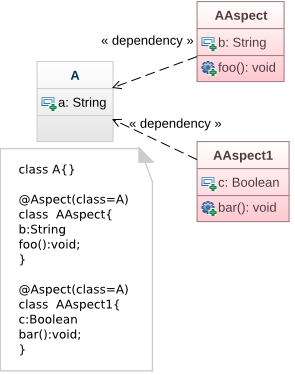
\includegraphics[width=0.75\linewidth]{chapter2/fig/library-developer-view.png}
\caption{Viewpoint of library implementor}\label{fig:library-view}
\end{subfigure}
\hspace{0.3cm}
\begin{subfigure}[b]{0.45\textwidth}
\centering
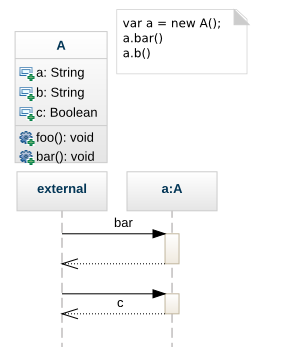
\includegraphics[width=0.75\linewidth]{chapter2/fig/user-view.png}
\caption{Viewpoint of library user}\label{fig:user-view}
\end{subfigure}
%\hspace{2.6cm}
\begin{subfigure} {\linewidth}
\centering
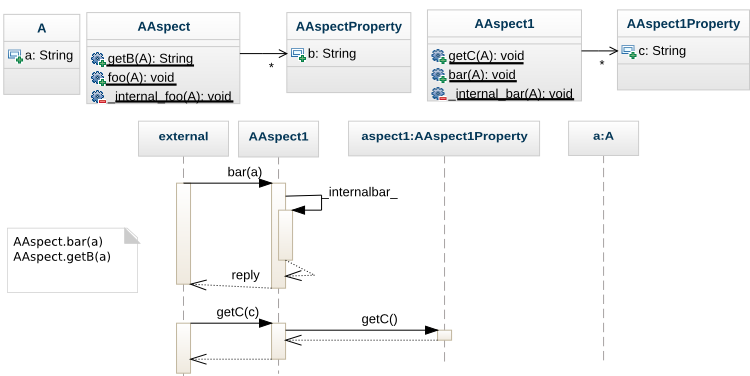
\includegraphics[width=0.9\linewidth]{chapter2/fig/tooling-view.png}
\caption{Tooling's view}\label{fig:tooling-view}
\end{subfigure}
\caption{Open-class mechanism in K3-AL, three views are shown: how the developer o the library see it (Fig \ref{fig:library-view}), how the user of the library see it (Fig~\ref{fig:user-view}), and how it is perceived by the tools (Fig~\ref{fig:tooling-view}).}
\label{fig:k3-diagram}
\end{figure}


\paragraph{The case of monitoring components}
In OSGi, a component framework, many bundles are deployed on top of a single JVM instance.
Due to the communication mechanism used in OSGi, where objects are routinely shared, it is complex to decide which bundle should be accounted for the consumption of a particular object.
A possible approach is deciding that an object $O$ is being consumed by a bundle if $O$'s class was loaded using the classloader $C$ associated with such a bundle.
Then, we can use this mechanism to monitor per-bundle memory consumption. 
However, a profiler must perform considerable amount of processing to collect such kind of data because it is not straightforwardly available in the JVM. 
%Since we know how to represent a bundle using Java concepts, this solution is feasible.
Given the widespread usage of OSGi, memory profilers often support collecting data regarding per-bundle memory usage.
Unfortunately, similar abstractions (components models), equally implemented atop of Java, are often not properly supported by such tools because they are not as popular as OSGi.
Hence, data must be manually aggregated when an application uses abstractions that are not supported by profilers; this is a considerable burden for developers.

The example of OSGi is also useful to highlight how some abstractions have specific requirements regarding resource consumption monitoring and reservation.
In the particular case of determining how many resources are being consumed by a bundle, it is noteworthy that there exist two ways of doing so when a bundle requests a service from another bundle.
Both approaches have pros and cons \cite{Miettinen2008,Maurel:2012:AME:2304736.2304763}.
In a first option, all resources used to satisfy a request are charged to the bundle that originally issued the request, no matter whether part of the computation is performed in other bundles.
In a second option, a bundle only consumes resources when it is executing its own code.
The important point is that, above the concern we present in the previous chapter regarding the mechanisms to support resource-aware programming, engineers also have to focus on features specific to each abstraction.

\paragraph{The problem at hand}
In this thesis we argue that a \textit{mismatch}, between the developer's view and the tooling's view, exists when the concepts managed by the developers are not clearly reflected in the tools.
This mismatch may complicate the development of applications, as well as prevent the correctness of software systems.
We identify in this thesis, two ways in which such a mismatch may affect software development when new software abstractions are heavily used and, at the same time, support for resource-aware programming is also required:

%\todo{This two points are really close, bad}
\begin{itemize}
\item The creation of new software abstractions poses challenges for software developers because abstractions may have requirements that are not addressed by generic developing tools.
In particular, tools, such as profilers, and runtime monitors, might require modifications in order to reduce the gap between the user's view and the tools' view.
The problem is how to efficiently reuse the generic mechanisms of existing approaches to handle the specific requirements of new abstractions.

\item Since new software abstractions are constantly being defined, there is an increasing pressure to ease the creation of abstraction-specific tooling support.
Simplifying the definition of tools in order to support new abstractions is the issue in this case. 
\end{itemize}

In the rest of this chapter, we extensively discuss both concerns.

\section{Dealing with abstraction-specific requirements} \label{sec:abstraction-specific-requirements}
As claimed in the previous section, when a new abstraction is defined, there is a gap between the capabilities of existing tools and users' expectations.
Therefore, it is necessary to reduce this gap by modifying generic tools to make them capable of dealing with specific features of new abstractions.

In this section, we present the challenges that emerge when tooling support for resource management is being built.
To do so, we discuss the topic in two ways:

\begin{enumerate}
\item  We present how the mismatch between existing tools and users' expectation continuously emerges due to the increasing usage of DSLs to build applications.
This serves both to further motivate the research, and to present in details the technical complexity an engineer may face when new abstractions are used.
%In general, most problems we find, when programs are written using DSLs and resource awareness is required, can also be found in other contexts where different kind of abstractions are used.

\item We describe the specific features of a concrete kind of abstraction - software components.
We do so because, despite of the fact that component-based software engineering is widely used in the industry, exiting approaches to support resource awareness still show limitations.
\end{enumerate}

The presentation aims at highlighting the type of modifications that might be required in order to make an existing resource management tool capable of dealing with concepts defined in a new abstraction.
To guide the discussion, the following elements are given for both, programs written using DSLs and component-based systems:
\begin{itemize}
\item A \textbf{brief description} of the main elements of the abstraction, focusing on those features that impact resource management. 

\item Illustrative cases of \textbf{implementations} of these abstractions \textbf{on top of MRTEs}.
For instance, it briefly mentions components models that support Java.

\item An analysis of how \textbf{resources are consumed} by each type of abstraction.

\item \textbf{Special characteristics of these abstractions} to take into account when support for resource-aware programming is implemented.     

%\item \textit{Example of differences among concrete abstractions.}
%Since there are, for example, many DSLs, this point aims at analyzing differences among them.
%In this way, we show the high degree of variability that might complicate the development of resource-aware solutions.
%Instead of providing an exhaustive list of differences, we only show an illustrative one.

\end{itemize}

Afterwards, the \textit{state of the art} on providing support for resource awareness for new abstractions and, in particular, for component models is presented.
This is done in the form of a summarized discussion of existing approaches. 
The section ends by analyzing the limitations in these approaches. 


\subsection{DSLs: land of hungry abstractions} \label{sec:DSL-on-MRTEs}

In Model-Driven Software Development (MDSD), models are abstractions of a software system and its environment~\cite{Stahl:2006:MSD:1196766, Fowler:2010:DSL:1809745}.
A model contains a limited amount of information of a real system; thus, its utility is restricted to the domain it represents.
The set of concepts and relationships that can be used in a concrete model are described in a Metamodel, which is also called Domain-Specific Language (DSL)~\cite{Fowler:2010:DSL:1809745}.
In this way, a DSL describes a specific domain (e.g., state machines, interface definition language); while a model is then a concrete state machine in a real application, or a description of how components in a system interact.

In their seminal work~\cite{Czarnecki2000}, Czarnecki and Eisenecker embrace a broad notion of ``language'' that encompasses what are now known as internal and external DSLs, but it also includes libraries of routines or classes that extend a programming language because they introduce new concepts and vocabulary.
This widely used notion of ``language'' is what we have in mind when we discuss the problems associated to resource consumption in DSLs.

An internal DSL is embedded into a general-purpose language (GPL).
Often, preprocessors and meta-programming facilities, of either a dynamically typed host language or a statically typed language with type inference, are used to seamless integrate the DSL into the host language.
Likewise, design patterns and reflection are used to implement some forms of internal DSLs, such as fluent APIs, and annotation-based languages.
On the contrary, a ``\textit{program}'' written using an external DSL requires a separated translation process (i.e., compilation) in order to produce an artifact that can be integrated as part of an application.
Both approaches have advantages and disadvantages that have been discussed elsewhere~\cite{Czarnecki2000, Stahl:2006:MSD:1196766}.
%Internal DSLs can leverage all the features of their host languages, and it is easy to use constructors of the DSL as extensions of the host language.
%However, the concrete syntax of an internal DSL must be carefully crafted to cope with the constrains in the host language's syntax.
%On the contrary, there is complete freedom in deciding the concrete syntax of external DSLs; as a designer you can even choose not to use a textual syntax.
%Another interesting point is that Integrated Development Environment (IDE) support for internal DSLs is limited to the support provided to the host language.

In a typical scenario, models are translated to source code written in some GPL to enable their subsequent compilation and execution.
However, models are also useful in other tasks such as generating test cases \cite{Kiffe2009,Gutierrez2015}, simulating a system behavior \cite{Broenink2012,brosig2015a,Bocciarelli2015425}, and formally verifying software properties \cite{Holzmann2004,Henriksson2005101,Moffett2013,DiGuglielmo20132013}. 
To write programs using a DSL (create models conforming to a metamodel), it is often necessary to use graphical~\cite{Kolovos:2009:RLA:1564600.1564699, Biermann:2006:GDI:2087202.2087244} or textual editors~\cite{Merkle:2010:TMT:1869542.1869564}.
In general, the definition of a new ``language'' is a complex task because, depending on the language features, it may involve the definition of a complete infrastructure to deal with the DSL (i.e., editors, compilers, and simulators).
Fortunately, approaches exist to ease the definition of DSLs.
For instance, Xtext~\cite{Eysholdt:2010:XIY:1869542.1869625} is a well-known tool that is useful for defining new external DSLs (or for extending existing languages).
It is an Eclipse-based framework which supports the definition of languages together with their syntaxes, semantic checkers, code generators and editors.

\paragraph{Support in MRTEs} 
As mentioned, concrete ``programs'' written in a DSL are typically translated to some host GPL.
This means that the DSL concepts are layered on top of concepts, such as \textit{classes}, \textit{objects}, and \textit{threads}.
Plenty of approaches exist for writing DSL-based applications that are transformed to execute on top of MRTEs; in particular, many solutions target Java.
For instance, the already discussed Xtext~\cite{Eysholdt:2010:XIY:1869542.1869625}, the Eclipse Modeling Framework~\cite{EMFModeling}, the meta-programming capabilities of languages such as Scala~\cite{Hofer:2010:MDL:1868294.1868307} and Clojure~\cite{Kelker2013} where internal DSLs can be defined and executed, the combination of annotations and annotation processor~\cite{Huang2008}, and intentional programming frameworks such as Meta-Programming System (MPS)~\cite{JetBrainsMetaProgrammingSystem(MPS),Voelter2014}.
Likewise, F\# applications, which execute in CLR, can use meta-programming support to write DSLs~\cite{Cheney:2013:PTL:2500365.2500586}; and the Boo language provides constructor that are easy to use for crafting DSLs~\cite{Rahien2010}. 

\paragraph{How abstractions consume resources} 
Naturally, the resource consumption of a ``program'' written in a DSL depends on the DSL itself.
If a language is only used to describe structures then a program would consume memory.
On the contrary, if a language only describes behavior, a program written using such a language would use CPU to perform the computation.

An example is useful to illustrate how a DSL consumes resources.
Figure~\ref{lst:state-machine} shows a program written in a state machine language that resembles a DSL described in~\cite{Voelter2010}.
In this DSL, states, events and transitions are concepts defined by the DSL, but the guard conditions and the actions have a behavior that, as can be seen in the example, is plain imperative code.
To evaluate such sections of a state machine, CPU time is required.
In this case, it is necessary to know the translational semantic of the language in order to properly measure the CPU consumption.

\lstdefinestyle{statemachinelang}{
  belowcaptionskip=1\baselineskip,
  breaklines=true,
  frame=single,
  xleftmargin=\parindent,
  language=C,
  showstringspaces=false,
  basicstyle=\footnotesize,
  keywordstyle=\bfseries\footnotesize\color{green!40!black},
  commentstyle=\itshape\color{purple!40!black},
  identifierstyle=\footnotesize\color{black},
  stringstyle=\color{orange},
  otherkeywords={StateMachine, state, states, events, on, initial},
  tabsize=2,
}

\begin{lstlisting}[caption={State machine to control the door of a bus.},label={lst:state-machine},style=statemachinelang,frame=single]
StateMachine BusDoorManager
	events open_door() stop_requested() bus_stops() time_elapsed() 
	states (initial = DoorClosed) {
		state DoorClosed:
			on stop_requested() => ReachingStop
		state BusStopped:
			on open_door() => DoorOpen { light.on; door.open; timer.wait }
		state ReachingStop:
			on open_door() => OpeningDoor {}
			on bus_stops() => BusStopped {}
		state OpeningDoor:
			on bus_stops() => DoorOpen { light.on; door.open; timer.wait }
		state DoorOpen:
			on open_door_requested() => DoorOpen {}
			on time_elapsed() => DoorClosed { door.close; light.off }
	}
\end{lstlisting}

In other cases, the translation process of a DSL may only generate a structure for each ``program'', without any associated behavior.
Hence, only memory is consumed by the execution environment to represent a concrete model at run time.
For example, suppose we define a language to represent plants using the L-System formalism~\cite{Prusinkiewicz1990}.
A plant created by Prusinkiewicz et al.~\cite{Prusinkiewicz1990} using L-Systems, is depicted in Figure~\ref{lst:OL-system-example}.
The structures generated by this language may be simple strings of symbols (see \ref{fig:l-system-generated}).
As can be appreciated, the memory consumed by a L-System depends on the number of iterations, the rules defined, and the concrete data structure used to store the symbols
(it can be a string of characters, a tree, a list, or an array).
The important point is that users of this language should see this kind of structures as black-boxes.


\lstdefinestyle{OL-systems}{
  belowcaptionskip=1\baselineskip,
  breaklines=true,
  xleftmargin=\parindent,
  language=C,
  showstringspaces=false,
  basicstyle=\footnotesize,
  keywordstyle=\bfseries\footnotesize\color{green!40!black},
  commentstyle=\itshape\color{purple!40!black},
  identifierstyle=\footnotesize\color{black},
  stringstyle=\color{orange},
  otherkeywords={contants, variables, initial, rules, iterations, angle, degrees, plant},
  tabsize=2,
}

\begin{figure}[ht]
\begin{mdframed}
\begin{subfigure}{0.45\textwidth}
\begin{lstlisting}[style={OL-systems}]
plant P0
	contants: + - [ ]
	variables: X F
	initial: X
	rules:
		X -> F[+X]F[-X]+X
		F -> FF
	iterations: 7
	angle: 20 degrees
\end{lstlisting}
\caption{DSL Code}\label{fig:l-system-code}
\end{subfigure}
\hspace{0.6cm}
\begin{subfigure}{0.45\textwidth}
\centering
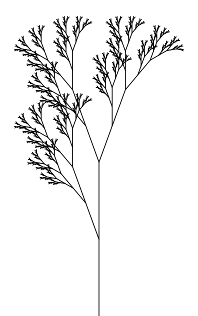
\includegraphics[scale=0.35]{./chapter2/fig/plant.png}
\caption{Graphical representation}\label{fig:plant}
\end{subfigure}
\hspace{2.6cm}
\begin{subfigure} {\linewidth}\centering
\begin{lstlisting}[language=java, basicstyle=\footnotesize, stringstyle=\footnotesize\color{green!70!black}]
String P0 = "FF[+F[+X]F[-X]+X]FF[-F[+X]F[-X]+X]+F[+X]F[-X]+X";
\end{lstlisting}
\caption{Java code generated after translation (two iterations instead of seven)}\label{fig:l-system-generated}
\end{subfigure}
\end{mdframed}
\caption{Simple OL-System to generate a plant in two dimensions. On the left, the OL-System is represented using a DSL, on the right we show the tree that can be generated using such OL-System, below is the representation in Java.} \label{lst:OL-system-example}
\end{figure}

An important \textbf{feature to consider} by engineers who implement support \textbf{for resource awareness},
is that languages do not always provide well-defined boundaries.
For instance, an internal DSL may be transformed into a list of statements of the host language without defining a new routine or thread.
In a case like this, instrumentation is the only mechanism that can be used to achieve CPU consumption monitoring.
Interestingly, interaction between parts of a application written using DSLs can also impact the way resource accounting is done.
In the state machine example previously discussed, a state machine might trigger events in another state machine by simple executing some actions in one of its transitions.
In a situation like that, a resource accounting framework should properly determine the change of execution context; unfortunately, implementing this can be computationally expensive. 

%\extracomment{TODO}{
%One paragraph to highlight how the problem we find with programs implemented using DSLs also exist when other mechanisms are used to define abstractions.
%}

%The \textit{state machine} and \textit{L-system} languages clearly reflect differences between DSLs.
%These differences are not surprising.
%Languages consume resources in different ways; some languages only consume memory while others consume CPU or other resources.
%The capacity to monitor the consumption of a program written using a DSL is related to factors such as,
%the specific meaning of the involved concepts,
%and the translational semantic of the language.

%\extracomment{TODO}{Add discussion on how to ad plugins for Eclipse MAT and VisualVM}

%Profilers: visualvm
%
%low-Level profiling technologies: JVMTI, DTrace
%
%In~\cite{Xu:2013:PML:2491509.2491511} the authors propose a framework to detect memory leaks associated with Java containers.
%To do so, the framework explores the status of each container object with the goal of identifying leak patterns.
%
%LeakBots~\cite{Mitchell03leakbot:an} is an automated tool to detect memory leaks. It makes heavy
%use of information collected from the heap in order to identify the more likely structures leading to a leak.
%These tools collect data from the heap in order to automatically pinpoint a particular memory issue.
%The methods to collect the data are handwritten for efficiency reasons.
%Lots of data collected in these works is also available with our approach.


\subsection{On how software components consume resources} \label{sec:components-oriented-resource-awareness}

Component-Based Software Engineering (CBSE) aims at developing applications by reusing independent units of software \cite{cbse-conference, Crnkovic2011}.
Through the utilization of components, connectors and configurations, CBSE reduces the complexity in the development and maintenance of systems \cite{xadl,Medvidovic:2000,VanOmmering-et-al-00}.
%In addition to economical benefits such as reducing time to market and development cost \cite{SZYPERSKI2002}, there are also technical advantages in using CBSE. 
One of its technical advantages is that it facilitates the management of dynamic architectures
~\cite{DBLP:journals/ase/NittoGMPP08, Johnson:2015:CSM:2735960.2735979}
because it simplifies the implementation of features, such as, self-organizing the structure of a system, and self-adapting its behavior
\cite{PanzicaLaManna:2012:LDU:2304736.2304764, Johnson:2015:CSM:2735960.2735979,Zhang:2009:MVD:1509239.1509262}.
Likewise, many works~\cite{cbse-conference} have shown the benefits of using component-based approaches in open-world environments~\cite{baresi2006toward, Caporuscio:2010:AIA:1985522.1985547, Perez-Palacin:2010:PAO:1712605.1712614}.

In a general sense, the concept that embodies the idea behind software components can be defined as follow
\cite{Crnkovic2011}:

\begin{description}
\item[Definition 1:] A \textit{Software Component} is a software building block that conforms to a component model. 
\item[Definition 2:] A \textit{Component Model} defines standards for (i) properties that individual components must satisfy; and (ii) methods, and possibly mechanisms, for composing components.
\end{description}

Plenty of diversity exists in current component models and frameworks \cite{Heineman2001, SZYPERSKI2002, Crnkovic2011}.
They tend to target different technologies, aim at different use cases, provide support for different concerns, and use different design principles.
Crnkovic et al. \cite{Crnkovic2011} propose properties that can be used to classify component models; we are interested in those models that have the following properties:

\begin{description}
\item[Modeling capabilities:] it is common to provide a mechanism for modeling the system architecture during the development phase; this results useful to reason about the system.
In addition, it is possible to support some form of reflection for querying the architecture of a system at runtime.
Component models, which include both features, are the target of our research.

\item[Deployment of components at runtime:] since, we are dealing with the problem of supporting resource awareness in open environments, we focus on component models that allow component deployment at runtime.
Many component models are able to cope with the necessity of adaptation through, for example, the deployment of new modules, the instantiation of new services, and the creation of new bindings between components~\cite{Porter:2014:RMC:2602458.2602471, Zheng:2014:RCC:2679601.2680405, Irmert:2008:RAS:1370018.1370036, Ghezzi:2010:QDD:2163764.2163774}.
\end{description}

Other properties worth mentioning in this thesis are those that describe how components communicate.
For instance,  whether the concept of \textit{port} is implemented; if there exists distinction between \textit{required} and \textit{provided interfaces}; characteristics of the \textit{interface language}; and what is the \textit{communication type} (synchronous, unicast, and others).
Our interest in these properties is limited to understanding what mechanisms are used to support interaction between components, how are these mechanisms implemented, and how this interaction affects the way in which we deal with resource consumption monitoring and reservation.

To guarantee properties regarding the behavior of components (and the systems built using them), contracts are used. 
According to \cite{Beugnard774917}, \textit{contracts} can be classified in four levels which, if
taken together, form a global contract; these are syntactic, behavioral, synchronization, and Quality-Of-Service (QoS).
Contracts based on the first three levels describe what can be done using a component and under which provisions.
They do not specify other properties, such as what resources would be consumed by a component to perform some action.
Nevertheless, a violation of QoS requirements breaks clients just as easily as a violation of a business rule.
If a provider is too slow in serving a request, client components will also be slow in achieving their goal.
These contracts, which express QoS and extra-functional properties, are used to control how many resources a component consumes.

In writing a contracts to express requirements regarding resource utilization, developers may profit of platform-independent mechanisms to describe the resources needed by components and component-based systems.
Indeed, writing contracts using platform-dependent metrics hinders its interpretation when components are deployed in a different execution environment.
For instance, if a contract expresses the fact that a component needs $n$ number of CPU cycles to handle a request, the value of $n$ may, in fact, represent different values depending on the architecture.
For this reason, using a metric, such as number of bytecode instructions executed, to describe a contract is useful in MRTEs.
This metric in particular has the following advantages:
\begin{itemize}
\item It is easy to control the admission of components because each platform knows how many bytecode instructions it is able to execute in an interval of time.
\item A portable framework for resource consumption monitoring is easier to implement.
\item Different measurements are easy to compare, even across platforms, because they use the same metric.
\end{itemize} 

Besides the metrics used, the exact interpretation of a contract is also a fundamental concern.
Contracts may express properties for just one component and a single type of resources, but they can also express how should be the usage of resources in more complex scenarios where different components and types of resources are involved.


\paragraph{Support for component-based engineering in MRTEs}
An important property of component models is its implementation support.
The discussion in this research is limited to those that have been implemented for MRTEs.
Several component models that provide support for MRTEs have been proposed in both the industry and the academy.
Among others, we can mention Enterprise Java Beans (EJB) \cite{OracleEJB3.0}, the Open Services Gateway Initiative (OSGi) \cite{OSGI:r5}, 
Fractal \cite{Bruneton:2006:FCM:1152333.1152345}, 
SOFA 2.0 (Software Appliances) \cite{Bures2006}, Palladio \cite{Becker:2010:PCM:1712605.1712651}, and Kevoree~\cite{morin09a,leger2010reliable}.
It is interesting how these component models have different properties when it comes to \textit{modeling capabilities}, \textit{architecture of the system supported}, and \textit{constructs for interaction among components}.
However, they also differ in how components are represented on top of MRTE concepts; in other words, they follow different approaches to implement the component framework itself.

\paragraph{How components consume resources}
Interestingly, components provide boundaries between different software entities, which are forced to communicate through well defined interfaces; it is then possible to write QoS contracts associated to these interfaces \cite{Beugnard774917}.

It is important to remember the difference between component type and component instance when we discuss the resource usage of these systems.
Indeed, instances may have a state while component types are stateless.
The distinction is important because all instances of a single component type share the same implementation.
As a consequence, it is not simple to define how a component consumes resources.
For example, the memory consumed by an instance includes those \textit{objects} used for the component framework to represent the instance itself, its ports, and bindings; it also includes the state of the component. 
However, it cannot include the memory used to store the component's code since it is shared among many instances.
Monitoring CPU and network consumption is even harder, because the code responsible for the consumption is shared.
To solve this problem, a context is associated with each component in order to determine at runtime the instance responsible for the execution of a given operation that is using resources.
Interestingly, the exact representation of this context depends on the component model, and it may impact the performance of component-based systems.
A common way to define this context, is associating a set of threads to a component.

To summarize, the resources consumed by a component comprise (but are not limited to): its state, the time-shared resources it uses (CPU, network), the space required to store data and code shared among all instances of a component type, and the temporary space needed to execute the component.       

\paragraph{Specific features to consider}
A first issue to take into consideration is \textit{how to account for resource consumption in the presence of interaction between components}.
Usually, components are organized as clients and providers, where a component (provider) performs operations on behalf of other components (clients).
It is then possible to account for resource consumption in two ways \cite{Miettinen2008,Maurel:2012:AME:2304736.2304763}:

\begin{description}

\item[indirect accounting:] all the resources consumed to serve a request that was originated in a component A are accounted to A (See Figure~\ref{fig:indirect-accounting}).
In other words, there is no resource consumption accounted to service providers.

\item[direct accounting:] the resources consumed during
interaction are accounted to the provider (See Figure~\ref{fig:direct-accounting}).
For instance, the CPU used by a code that belongs
to component A is accounted to A, no matter if the code is executed on behalf of a client.
\end{description}

Both ways have advantages and disadvantages.
In the case of direct accounting, if a provider is
called in an endless loop, the resource usage will be accounted
to the provider instead of to the client that executes such a loop.
On the contrary, if a service is poorly implemented, in indirect accounting the user of the service is identified as the responsible.

\begin{figure}[ht]
\begin{subfigure}{0.45\textwidth}
\centering
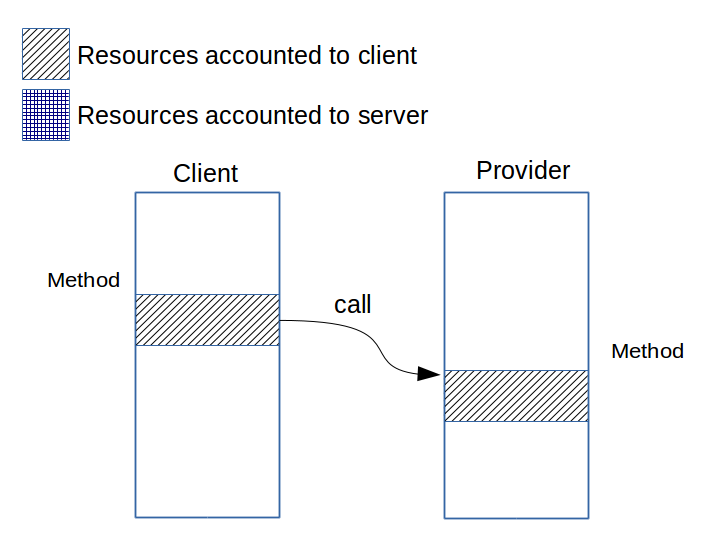
\includegraphics[scale=0.35]{./chapter2/fig/indirect-accounting.png}
\caption{Indirect Accounting}\label{fig:indirect-accounting}
\end{subfigure}
\hspace{0.6cm}
\begin{subfigure}{0.45\textwidth}
\centering
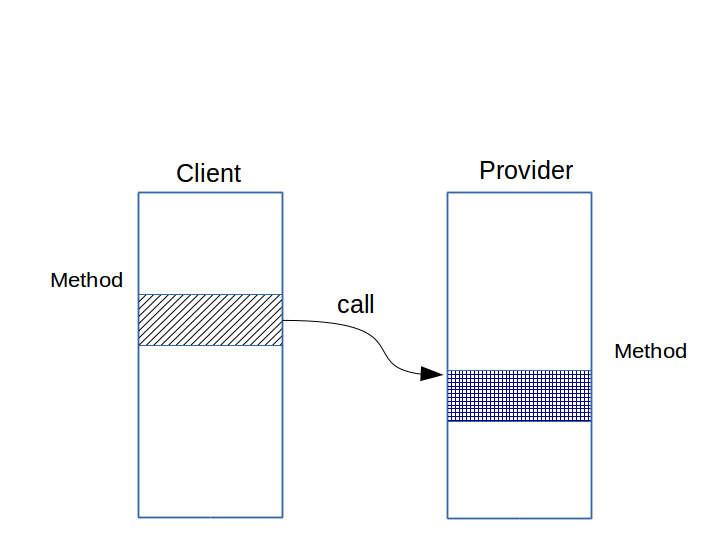
\includegraphics[scale=0.35]{./chapter2/fig/direct-accounting.png}
\caption{Direct Accounting}\label{fig:direct-accounting}
\end{subfigure}
\caption{The two mechanisms to account for resource consumption when components interact.} \label{fig:accounting-methods}
\end{figure}


Similarly, two criteria exist to account for memory consumption in component-based systems.
Usually, components interact, during this interaction they exchange objects that are typically created on one side of the interaction (e.g., a service component creates new objects in response to clients' requests).
Indeed, a component may allocate space for an object. pass it to a client, and then forget about it.
In that case, it is not clear what component should be accounted for the memory consumed by that particular object; it can be either the client or the original allocator.
Both approaches have pros and cons.
The intuition dictates that if a component is preventing an object of being collected it should be accounted for that particular block of memory.
However, such an approach may be dangerous if a buggy (or malicious) provider creates objects unnecessarily big, sends them to clients, and forgets about them; in that case, it would be hard to identify the provider as the source of excessive consumption. 
Most existing solutions for memory consumption always follow on of the two criteria.

A second aspect is to decide \textit{where should be implemented} the mechanism for resource consumption monitoring and reservation.
Essentially, this consists in, selecting which actors implement the mechanism and policies to manage resources, and deciding if the actors collaborate to achieve their goal \cite{Crnkovic2011}.

Many component models provide no facilities for managing EFPs.
The mechanism used to handle a property is left to the designers of each application.
This facilitates the creation of EFP management policies that are specifically tuned towards a system, and also allow the usage of multiple policies in a system.
However, the fact that such policies are not
standardized (and are fully implemented in components) may be a source of architectural mismatch between
components.
The compatibility of components is improved if the
execution platform provides standardized facilities for managing EFPs.
However, components still need to know EFPs affect their functioning in order to guide the manner
in which EFPs are handled.

In another approach, components are designed to address only functional aspects and not EFPs.
Thus, in the execution environment, these components
are wrapped in a container that has the knowledge on how to manage EFPs.
Containers can either be totally in charge of managing EFPs or
they can interact with a mechanism in the component framework that manages EFPs.
This approach is a way of realizing separation of
concerns in which components focus on functional aspects
and containers concentrate on extra-functional aspects.

%\paragraph{Example of differences among concrete abstractions}

Finally, some differences among component models impact the implementation of mechanisms for resource consumption monitoring.
For instance. Kevoree and OSGi provide different methods for interaction between components.
In Kevoree, components communicate with each other through ports.
It is straightforward to identify in the code when a component is requesting a service because a single interface (port) is used to do so, no matter if a component is using different ports. 
As a consequence, an automated tool can easily instrument the code to detect when components are communicating.
On the contrary, OSGi uses plain Java interfaces and objects to connect bundles.
In that cases it is more complex to detect when components are communicating because a bundle can communicate with several services using different interfaces. 

%\subsubsection{Extra-functional Properties} \label{sec:efp-resources}
%
%According to \cite{Beugnard774917}, contracts can be classified in four levels which, if
%taken together, form a global contract; these are syntactic level, behavioral level, synchronization level, and Quality-Of-Service level.
%Contracts based on the first three levels describe what can be done under which provisions.
%They do not specify other properties such as how long it would take to service a request or what other resources, besides time, would be consumed by a component in order to perform some action.
%Nevertheless, in real scenarios, a violation of extra-functional
%requirements can break clients just as easily as a violation of, for instance, a business rule. 
%If a provider is too slow in performing a function, any client component will also be slow in achieving their goal.
%Without using contract on QoS to control performance, it can be hard to identify what components are underperforming. 
%Beside time, components have to respect other resource limitations such as excessive heap storage and network usage.


%\subsection{Component Models}
%
%In the next section, we provide a very brief overview of some component models and their main characteristics.
%The discussion is limited to component models that have been either designed from scratch or implemented to target MRTEs.
%Since we are interested in software systems that evolve at runtime, the discussion is also limited to component models that allow component deployment at runtime.
%The list is not exhaustive; instead, it should be understood as a provision of some characteristic examples.
%Nevertheless, a component model - Kevoree -  is discussed in further details because the contributions in chapters \ref{chp:scapegoat} and \ref{chp:squirrel}
%are implemented and evaluated using such a component model.
%
%\paragraph{Enterprise Java Beans (EJB)} \cite{OracleEJB3.0} envisions the construction of object-oriented and
%distributed business applications in trying to hide to developers the underlying complexity of common operations such as transactions processing, persistence,
%concurrency, and interoperability.
%It also aims at the improvement of component reusability in providing the so called EJB-jars to package components.
%An EJB container holds two major types of components to match the needs of different applications: SessionBean, and MessageDrivenBeans.
%Each of these beans is deployed in an EJB Container which is in charge of their management at
%runtime (start, stop, activation or deactivation).
%Starting with EJB 3.0, annotations are heavily used for dependency injection to simplify configuration and integration of heterogeneous systems. 
%In order to achieve this, EJB technology use the Java programming language.
%
%\paragraph{The Open Services Gateway Initiative (OSGi)} \cite{OSGI:r5} is a consortium of industrial partners working together to
%define a service-oriented framework with ``open specifications
%for the delivery of multiple services over wide area networks to local networks and devices''.
%In the OSGi's component definitions, there is a clear distinction between a unit of
%composition and a unit of deployment; the former is known as service while the latter is called bundle.
%OSGi offers a flexible architecture of systems that can dynamically evolve during execution time.
%This implies that in the system, components can be added, removed or modified at run-time.
%Thus, there is no guaranty that a service provided at a certain time will be still provided later.
%Being built on Java, on which it heavily depends, OSGI is platform independent.
%
%%\paragraph{Fractal} \cite{Bruneton:2006:FCM:1152333.1152345} is a hierarchical and reflective component model with sharing.
%%Components in this model can be endowed with arbitrary reflective capabilities, from plain black-box objects to
%%components that allow a fine-grained manipulation of their internal structure.
%%The paper describes JULIA, a Java implementation of the model, a small but efficient runtime framework, which relies on
%%a combination of interceptors and mixins for the programming of reflective features of components.
%%The paper presents a qualitative and quantitative evaluation of this implementation, showing that
%%component-based programming in FRACTAL can be made very efficient. 
%
%\paragraph{Fractal} \cite{Bruneton:2006:FCM:1152333.1152345} intends to cover the whole development lifecycle (design, implementation, deployment and maintenance/management) of complex systems.
%It comes up with features such as nesting, sharing of components and reflexivity.
%In other words, a component may respectively be created from other components, be shared between components and describes its own behavior.
%Fractal aims at providing an general model that can be tuned to fit a large variety of applications and domains.
%Hence, nothing is fixed in Fractal.
%Actually, since the component model is language and platform independent, it is possible to leverage domain-specific 
%For instance, there exists a C-implementation called Think \cite{Fassino:2002:TSF:647057.713860}, 
%a Java-implementation called Julia \cite{Bruneton:2006:FCM:1152333.1152345}.
%Fractal can be seen as a generic component model which intends to encompass other component models.
%
%
%\todo{READ UNTIL THIS POINT}
%
%\section{State of the art of resource management for components} \label{sec:component-leverage}
%\begin{itemize}
%\item Describe las soluciones de kouther
%\item generacion de contenedores
%\item generacion de canales de comunicacion
%\item ver que mas se puede describir
%\end{itemize}
%
%
%Franz Brosch, Heiko Koziolek, Barbora Buhnova, Ralf Reussner: Architecture-Based Reliability Prediction with the Palladio Component Model. IEEE Trans. Software Eng. 38(6): 1319-1339 (2012)
%
%Sam Malek, Marija Mikic-Rakic, Nenad Medvidovic: A Style-Aware Architectural Middleware for Resource-Constrained, Distributed Systems. IEEE Trans. Software Eng. 31(3): 256-272 (2005)
%
%Anne Koziolek, Ralf Reussner: Towards a generic quality optimisation framework for component-based system models. CBSE 2011: 103-108
%
%Marco Autili, Paolo Di Benedetto, Paola Inverardi: Context-Aware Adaptive Services: The PLASTIC Approach. FASE 2009: 124-139
%
%Mauro Caporuscio, Antinisca Di Marco, Paola Inverardi: Model-based system reconfiguration for dynamic performance management. Journal of Systems and Software 80(4): 455-473 (2007)
%
%Marco Autili, Paolo Di Benedetto and Paola Inverardi, Hybrid Approach for Resource-based Comparison of Adaptable Java Applications (2012), in: Journal of Science of Computer Programming (SCP)

\subsection{State of the art on dealing with abstraction-specific features}

This section presents a several approaches that tackle the problem of providing tooling support for developing applications using new software abstractions.
In particular, it discusses some solutions for debugging domain-oriented abstractions.
Furthermore, this section describes several mechanisms to monitor how components consume resources and to isolate such consumption.

\paragraph{Providing resource awareness support for DSLs}
Among the development tools that help to software maintenance, debuggers and profilers generally support mainstream concepts such as \textit{classes}, \textit{objects}, \textit{methods}, and \textit{call stack}.
Using them, it is possible to determine, at some extent, how applications are consuming resources.
However, we have found that limited support exists for extending the usage of these tools in order to make them understand more specific concepts (e.g., classes representing the business logic of an application, or a design pattern).
In other words, they are not fully capable of dealing with resources at per DSL level.
Yet, some related works do exist; they aim at reducing the gap between the developer's view and the tools' view.
In particular, the problem of offering debugging support for DSL constructs have been discussed.
In Xtext~\cite{Eysholdt:2010:XIY:1869542.1869625}, languages that produce code in the base language (i.e., Java) may profit from mostly automatic debugger support.
When the newly define DSL is transformed into the base language, the system keeps traces between the two models (source and destination).
Using these traces, a debugging infrastructure is able to identify what constructor is being executed in the original DSL.
Meanwhile, Voelter \cite{Voelter2010} discusses how to add debugging capabilities to a DSL when the MPS language workbench is used.
In this case, no trace model is required; instead, every concept of a language that requires debugging support must implement a set of interfaces to guide a generic debugging framework.
Similar works have been conducted \cite{vandenBrand:2005:TGD:1705513.1705667} for the ASF+SDF Meta-Environment \cite{vandenBrand20013}, defining a generic debugging framework that can be customized for DSLs.
Finally, mechanisms to build various tools for new languages are described in \cite{Henriques2005}.
Based on attribute grammars, and implemented using the LISA system \cite{Mernik2002}; the tools proposed include editors, inspectors, debuggers and visualizers.

\paragraph{Component-based systems}

Many works address the issue of supporting resource consumption monitoring in component-based systems.
In addition, some existing approaches present solutions for the isolation of resource consumption among components running on top of a single MRTE instance.
Unfortunately, most approaches are limited to a specific component model; in particular, a considerable amount of work exist to solve the problem for both EJB and OSGi.

\textit{EJBMemProf}, a framework for profiling the memory consumption in EJB is presented in \cite{Meyerhoefer2005}.
The main idea of this framework is instrumenting applications' code to trigger an event each time an object is allocated; in response to such an event the framework identifies the component responsible for the allocation.
%The main idea is executing an event handler each time a new object is created; such a handler is responsible of identifying the bundle that allocated the object.
A set of rules that guide this identification process is discussed by the authors, and their accuracy evaluated.
Unfortunately, the overhead of the system is too high because, as part of these rules, the class name of each allocated object is compared against the package name of each component (this impacts the performance even if \textit{hashes} are used to compare \textit{strings}).
As a consequence, using the framework in a production environment is not possible.
Instead, this tool aims at supporting the development of component-based software.
Similarly, an approach to measure the execution time of EJB components is proposed in \cite{Meyerhofer05towardsplatform-independent}.
In this solution, engineers manually select those parts of a component that may be responsible for most CPU consumption at runtime.
These parts are then profiled in a development environment; the resulting data is combined with a description of the deployment platform to estimate what would be the execution time in the deployment platform.
Finally, a mechanism for measuring the response time of components, as well as the invocation tree, is discussed by Meyerhoefer et al. \cite{Meyerhoefer2007}.
This approach uses interceptors to collect data about how components calls each other.
It is intended to be use as a development tool.

%\textbf{Resource monitoring in EJB}
%
%TestEJB: response time measurement and call dependency tracing for EJBs
%
%In this paper we present how to conduct performance related analyses of component-based applications and how to derive call dependencies between software components in the TestEJB framework. This framework facilitates an interceptor-based approach to measure selected properties of components following the Enterprise JavaBeans specification. Amongst its advantages are the lightweightness and transparency to the application as the measuring sensors simply gather timestamps and additional metadata at selected positions inside a component-based application. Using basic database support, it is possible to generate invocation trees and calculate response- and run-times of a component and its methods while accounting for the overhead introduced by the framework itself. Therefore, the developer is offered a useful tool for benchmarking selected components as well as monitoring the interactions of components with the application server and amongst themselves.
%
%TESTEJB – A Measurement Framework for EJBs\cite{TESTEJB2004}
%Specification of Quality of Service (QoS) for components can only be done in relation to the QoS the components themselves are given by imported components. Developers as well as users need support in order to derive valid data for specification respectively for checking whether a selected component complies with its specification. In this paper we introduce the architecture of a measurement framework for EJBs giving such support and discuss in detail the measurement of the well understood property of response time.

Monitoring the resource consumption of OSGi bundles has also been addressed.
For instance, Miettinen et al. \cite{Miettinen2008} present a framework to measure CPU and memory usage of OSGi bundles.
This framework relies on some modifications to an existing OSGi platform in order to identify which bundle is consuming a given resource.
Such a modification creates a unique \textit{ThreadGroup} for a each bundle; since each object allocation and method execution is performed by a \textit{thread}, it is possible to figure out the bundle responsible by simple looking at the \textit{ThreadGroup} of the thread.
Alas, this approach suffers of considerable performance overhead because it extensively uses JVMTI and bytecode rewriting to detect resource usage (See previous Chapter).
In \cite{Maurel:2012:AME:2304736.2304763}, the authors propose an approach to reduce the overhead induced when CPU consumption is monitored; this is an adaptive monitoring system that is able to dynamically tune the accuracy of monitoring mechanisms depending on detected performance issues.
This solution is built on the idea of creating proxies that are responsible for detecting invocations, and also on the usage of localized CPU sampling.
The experiments show an overhead of 2\% when idle (the lightweights monitoring mode) and 20\% when completely active.
Memory consumption monitoring in OSGi execution environments has also been discussed in \cite{Attouchi:2014:MMM:2602458.2602467}, where the authors argue that some information regarding the \textit{business logic} is required to properly estimate the resource consumption of interacting bundles that belong to different stakeholders. 
To encode that information, they propose a DSL that describes what component must be charged for a given consumption when two components interact; this effectively increases the accuracy of the monitoring framework.
Unfortunately, the approach requires a modified JVM, and a persistent overhead is induced (up to 46\%) because the framework cannot be deactivated.

Other approaches address the issue of providing resource isolation between OSGi bundles.
In \cite{Kuroda2014}, the authors propose a memory isolation method for OSGi-based home gateways.
The method isolates the memory consumption of bundles without the need to modify bundles or the OSGi framework and has minimal overhead costs.
It does so by modifying the JVM (object layout, allocator, and the garbage collector) in order to evaluate, after each allocation, whether the bundle responsible for the allocation is violating some developers-defined limits on resource usage.
Meanwhile, I-JVM \cite{dsn/09/geoffray/ijvm} is a JVM that provides isolation between OSGi bundles.
In addition to avoiding unintended object sharing, the approach also tackles the issue of resource consumption monitoring for components; this is meant to, for instance, be used by administrator to avoid denial-of-services attacks.
The experimental results show an overhead of 16\% on inter-bundle calls.
Likewise, the problem of isolating CPU consumption in OSGi execution environments in order to support real-time component software development is discussed by Richardson et al. \cite{Richardson2009}.
The idea is to use the Real-Time Specification for Java (RTSJ) to support CPU isolation; this also requires modifications to the OSGi framework.
The authors claim that just using RTSJ is not enough to ensure real-time properties of applications when the OSGi framework is used to build them.
Besides the arguments to justify such a claim, a solution to achieve CPU isolation is presented.

Profilers such as Eclipse MAT and VisualVM offer limited support to perform memory consumption monitoring for mainstream component models (OSGi and EJB).
They do so by providing built-in subsystems that are able to process Java memory dumps to calculate the per-component consumption.
Due to the need of processing the complete memory dump, the performance overhead is considerable. 

%\textbf{Resource isolation in Component-RTSJ}

%Providing temporal isolation in the OSGi framework .
%The OSGi Framework is a run-time environment for deploying service-containing Java components. Dynamically reconfigurable Java applications can be developed through the Framework's powerful capabilities such as installing, uninstalling, updating components at run-time, and allowing the substitution of service implementations at run-time. Coupled with the capability to be remotely managed, the OSGi Framework is proving a success in a variety of application domains. One domain where it is yet to make an impact is real-time systems. Despite the fact that OSGi components and services can be developed using the Real-Time Specification for Java (RTSJ), there are still a variety of problems preventing the use of the Framework to develop real-time systems. One such problem is a lack of temporal isolation. This paper focuses on how temporal isolation can be provided in the OSGi Framework as a first step towards using the Framework to developing real-time systems with the RTSJ.
%(Usa RTSJ y un OSGi framework modificado)

%Towards memory management for service-oriented real-time systems\cite{Richardson2010}
%Dynamically discoverable units of software (services) are the centerpiece of service-oriented architecture (SOA). Such dynamic software architectures closely match the dynamics of businesses, and for that reason, SOA is becoming an increasingly important approach to the development of software. However, one aspect of deploying such dynamic software, that is frequently neglected, is the impact that it has on the availability of hardware resources such as CPU utilization and memory consumption. All software systems require the system load to be controlled in order to provide the service user with some level of quality-of-service. Furthermore, one type of software, which is particularly difficult to develop and would certainly benefit from the use of service-orientation, is real-time systems. Such systems, however, require resource guarantees and therefore are currently prohibited from using service-orientation in their design.
%In this paper we propose solutions to the problems relating to providing memory management in service-oriented real-time systems (RT-SOA).
%( memory management approach for RT-SOA allowing
%the memory requirements of threads to be calculated and used to
%generate GC parameters, only allowing threads to be admitted into
%the system when the addition of the thread will not cause memory
%to be exhausted, and of course, only when there is sufficient CPU
%for the threads to execute their own application code )

%\cite{Jung:2011:LAI:2000292.2000296}
%
%Architecting Fault-tolerant Component-based Systems: from requirements to testing
%
%A New Component Concept for Fault Trees
%
%Fault-Tolerance for Component-Based Systems - An Automated Middleware Specialization Approach
%
%otra cosa
%\cite{SZYPERSKI2002,Lau:2014:SCM:2602458.2611456}


\subsection{Discussing the state of the art}

In reviewing the state of the art, we have found some limitations on how existing solutions deal with specific features of abstractions.
In this section we discuss such limitations:


\begin{description}

\item[Limited support for resource accounting in component-based systems] There are several approaches for monitoring how individual components use resources.
However, they are limited and inefficient.
First, most of them only target mainstream component models such as OSGi and EJB; this is a fact noteworthy because it is not clear whether the ideas behind existing approaches can be applied to other component models.
The second and more important problem is the considerable overhead induced by these solutions.
In the case of memory consumption accounting, the best results we found show a persistent overhead of 46\% (medium).
By comparison, experiments of CPU consumption accounting show a lower overhead of 20\% when \textit{sampling} is used.
In many scenarios, these overheads are unacceptable. 

\item[Sub-utilization of information about the architecture of systems].
Actually, all approaches use rudimentary information about the architecture of the system that is running on top of the component framework.
In other words, they are able to determine how each component consumes resources (regardless of the accuracy).
As shown in \cite{Maurel:2012:AME:2304736.2304763}, it is possible to use information on how components are connected (their dependencies) to improve the monitoring accuracy.
Similarly, Attouchi et al. \cite{Attouchi:2014:MMM:2602458.2602467} show how to use the knowledge about the \textit{business logic} (in particular how components interact) to properly determine what component should be accounted for the consumption of an object.
Nevertheless, we have not found results showing how to reduce performance overhead by using information about the architecture of component-based systems. 


\item[Non-portable solution for resource isolation] Existent approaches to provide per-component resource consumption isolation require a modified MRTE.
In practice, this prevents the adoption of these approaches in production environments; due to the cost of maintaining a customized MRTE, and the complexity of keeping it up to date, some managers with limited budget may decide that these solutions are not acceptable.

%\item Only widely used component models such as OSGi, and EJB, have support for resource management.

\item[Wrongly assume that resource consumption is homogeneous]
Usually, components consume resources in different ways; some of them require CPU while other are memory or IO consumers.
However, many approaches to resource consumption and reservation are built without taking this into consideration; in short, they manage resources in the same way for all components.
This may have negative consequences in some cases.
For instance, some monitoring frameworks to calculate CPU consumption induce a persistent overhead in all components, even if only one of them is consuming too much CPU.
In the same way, solutions tend to use fixed mechanisms for monitoring and reserving resources, but we show in the previous chapter that some mechanisms are better for handling some kind of resources even if they are not able to manage all resources. 
It is our belief that adaptive mechanisms are preferable because, by analyzing the requirements and observing the status of a system, they are likely capable of reducing the overhead.
%Las soluciones son handcrafted y staticas, no se adaptan a lo que los componentes necesitan realmente (contrario a Squirrel y Scapegoat)\

\item[Limited capabilities for building tooling support] Debuggers, simulators and interpreters have been proposed as tools to support the maintenance of software written using DSLs; however, as far as we know, no profiler that specifically aims at reducing the gap between DSLs and base language have been presented.
It is worth mentioning that some general profiling frameworks can be used to ease the construction of profilers, even if they do not specifically address DSLs; these mechanisms as well as their limitations are discussed hereafter.

\end{description}

\section{Easing the construction of resource management tools} \label{sec:easy-tools-contruction}

As we already mentioned, the definition of new abstractions is common in software development (for example, using DSLs).
Sometimes, it is useful having tools to check how instances of these abstractions consume computational resources.
Unfortunately, building such tools is not a simple tasks.
It is then necessary to provide a ``simpler'' mechanism to build tooling support for abstractions.

Resource consumption monitoring is a form of dynamic analysis, and there are many approaches that tackle the issue of simplifying the definition of dynamic analysis tools.
Unfortunately, we have found fewer mechanisms to ease the construction of resource reservation tools \cite{mueller}.
Due to this fact, we mostly discuss in this section the problem of supporting resource accounting. 

In this section, we first present some approaches that aim at easing the construction of dynamic analysis tools.
We do so by describing the following dimensions for each approach:

\begin{description}
\item[Generality] Indicate the expressive power of the approach. We only consider two values: \textit{arbitrary} and \textit{limited}.

\item[Ease of use] We argue that the possible values are \textit{already known language}, \textit{new DSL}, \textit{require specific knowledge of the MRTE}.

\item[Performance Overhead] As in the previous paragraph we use the values \textit{low}, \textit{medium}, and \textit{high}.
Likewise, these values are taken from the literature review.
\end{description}

In Section~\ref{sec:discussing-tools-to-ease-construction}, we briefly discuss the limitations of such approaches.


\subsection{Flexible implementation of dynamic analysis tools}

One of the most tedious and error-prone tasks, when building tooling support for dynamic analysis, is dealing with low-level details such as, bytecode instrumentation.
If dynamic analysis tools are built from the scratch, developers are forced to focus on mastering details of the execution platform, when in fact, they are interested in implementing high-level ideas.
To address this issue, various approaches have been proposed; they can be clustered into three categories: instrumentation frameworks, high-level APIs for bytecode manipulation, and aspect-oriented tools.

\paragraph{Instrumentation frameworks}
Several instrumentation frameworks for MRTEs have been proposed.
In \cite{Liang1999}, the authors propose the JVM Profiling Interface (JVMPI); a set of low-level facilities built-in the JVM to trigger notifications when certain events occur during application execution.
Although the events reported only provide primitive information, such as \textit{method invoked} and \textit{thread created}, this basic data can be used along other infrastructure to build more powerful tools.
Severe limitations prevented the success of JVMPI (deprecated in favor of JVMTI): performance impact on the JVM, the relatively low-level interface provided, and the limited capabilities to detect fine-grained events.
These limitations are partially addressed in \cite{Maebe06javana:a} where a framework called Javana is proposed.
In specific, Javana proposes further modifications to the JVM to detect more events.
Additionally, it aims at easing the construction of efficient user-defined profilers by providing a generic instrumentation framework which can be adapted to specific needs.
To do so, users define a profile using an aspect-inspired DSL where \textit{pointcuts} represent the events of interest for a profilers, and advices, which are written in \textit{C/C++}, are in charge of collecting data on the dynamic behavior of a program.
Besides the problem of requiring a modified JVM, this approach also has other disadvantages such as demanding a deep understanding of the JVM.

A profiling framework that instruments Java programs at the bytecode level to build context-sensitive execution profiles at runtime is proposed in \cite{Binder2005}.
The framework includes an exact profiler as well as a sampling profiler.
Users can define their own profilers using a provided infrastructure for program transformation.
The most interesting point is that profilers are written in pure Java; this lowers the barrier for Java developers who devise customized profiling strategies.
Finally, Reiss proposes a framework~\cite{Reiss:2008:CDP:1383559.1383566}, DYPER, to organize and schedule the execution of monitoring agents.
Each agent (so-called proflet) is able to obtain data, regarding some properties, using two approaches.
Through sampling the data collected have poor quality, while data collected using instrumentation are very detailed.
The framework schedules the execution of proflets to guarantee a bound in the overhead of monitoring resource consumption.
To perform the scheduling, each proflet provides an estimates of both the expected application overhead and the time needed to set up the detailed monitoring; this information is used to dispatch the execution of a detailed collection of data.
In practice, this is a form of adaptive monitoring where mechanisms with high overhead are executed only when possible.
Proflets are built using either Java or C, and they can be composed in order to collect more complex data.
The main limitation of this approach
%, besides from the fact that no experimental validation regarding the overhead is provided, 
lays on the difficulty of properly estimating the overhead of proflets.

\paragraph{High-level APIs for bytecode manipulation}
The use of bytecode rewriting techniques to build dynamic analysis tools have leaded to the development of high-level APIs for bytecode rewriting.
For instance, ASM~\cite{Bruneton2002,Kuleshov2007} is a Java bytecode manipulation and analysis framework written itself in Java.
It is useful to transform classes directly in binary form.
To do so, it provides methods to traverse the binary code of Java classfile that allows users to create custom transformations.
Alas, it requires considerable knowledge regarding the JVM specification.
In particular, it is mandatory to understand the Java instruction set, how are they executed, and the basic structure of a classfile in Java.
By comparison, Javassist \cite{Javassist1999} simplifies Java bytecode manipulation.
It is a class library for editing bytecodes in Java; however, unlike ASM, it provides a source level API: to transform a classfile without knowledge of the specifications of the Java bytecode.
For example, you can specify what bytecode to insert in an existing class by using plain Java source code - Javassist compiles it on the fly and inserts it on the class being transformed.

\paragraph{Aspect-oriented tool construction}
The collection of data for a given dynamic analysis can be easily understood as a crosscutting concern.
Because of this, researchers have been attracted by aspect-oriented solutions.
Indeed, aspect-oriented frameworks already provide the mechanisms to i) specify multiple points of interest in the binary code of an application, and ii) execute handlers when the program counter reaches these locations.
In other words, by simply defining aspects (\textit{pointcuts} and \textit{advices}), developers can focus on the high-level ideas of dynamic analysis.
Nonetheless, aspect-oriented solutions are not flawless; some limitations have prevented its adoption in this field.
An interesting evaluation of the positive and negatives points of using aspect-oriented dynamic analysis is presented in \cite{Pearce:2007:PA:1248445.1248448}.
In addition to four dynamic analysis presented and evaluated (showing medium or high overhead), the authors also discuss how the \textit{pointcuts} of AspectJ are not sufficient to achieve better performance nor to create any type of analysis.
The issue of improving the performance is tackled by Binder et al. \cite{Binder:2006:FEM:1173706.1173733}.
In their work, the MAJOR~\cite{Villazon20111015} framework, an aspect weaver that enhances AspectJ with support for comprehensive weaving, is extended to guarantee fast sharing of values between aspects.
This simple addition is enough to reduce the performance overhead of some dynamic analysis.

DISL~\cite{Marek:2012:DEL:2162037.2162046,Marek2012} is a domain-specific aspect language for bytecode instrumentation; it uses annotations and plain Java to describe what a dynamic analysis tool must do.
The novelty of this approach is that new \textit{joinpoints} and \textit{guard conditions} can be defined using the Java language along some annotations.
It is then possible to collect data which is not accessible using a standard framework such as AspectJ.
Unfortunately, to define new \textit{jointpoints}, some knowledge of JVM internals is required.
Finally, in an effort to overcome the limitations of specific aspect weavers, which prevent using them to implement arbitrary dynamic analysis tools, Achenbach et al.~\cite{Achenbach:2010:MPD:1939399.1939415} propose an approach to customize aspect weavers.
When a new concrete weaver is built, the developer can choose arbitrary locations in the program as \textit{joinpoints}.
In the same way, different strategies to weave \textit{advices} can be implemented.
Implemented in Ruby, the approach is evaluated through the definition of a debugger and a testing tool.

\paragraph{Memory profilers}
Other approaches focus on profiling the memory usage of applications.
Memory profilers that are widely used in the industry provide languages to perform mostly arbitrary queries on the set of objects loaded in the heap.
For instance, in Eclipse MAT \cite{Biermann:2006:GDI:2087202.2087244} and Visual VM \cite{OQL-visualvm}, users can write queries in OQL (a SQL-like language) to retrieve information.
Despite of the fact that few constructors of OQL are really implemented in Eclipse MAT, this approach would allow, in theory, collecting practically any information contained in the heap.
Similarly, YourKit \cite{yourkit} provides a language based on set theory to filter objects with specific properties; this language is used when no built-in memory analysis can provide the desired data.
Besides providing query languages, mainstream profilers also support the development of extensions (e.g., plugins written in Java); these extensions essentially traverse the graph of objects in a heap dump to collect information.
Alas, both queries and extensions require costly operations - a complete dump of the heap, and a step to preprocess the dump; only after these operations, the frameworks are capable of executing queries.
In DeAl~\cite{Reichenbach:2010:GCE:1869459.1869482}, the authors propose a language to compute heap assertions at garbage collection time.
The design of this approach aims at guarantee a low performance overhead.
To ensure such a property, the language is only able to compute boolean outputs; while resource consumption monitoring, for instance, needs to compute values of integer type.
DeAl is a purely declarative language; in exchange for the declarative style and the focus on assertions, some properties about the performance of queries written in DeAl can be formally proved. 

\subsection{Discussing the limitations} \label{sec:discussing-tools-to-ease-construction}

Although there exist many approaches that aim at reducing the complexity of writing tools to support resource-aware programming, in reviewing the literature we have found some limitations that prevent using such solutions in production environments.
In particular, the identified limitations are related to the three aforementioned dimensions, \textit{generality}, \textit{ease of use}, and \textit{performance overhead}.
%We can assess the overall quality of a mechanism by looking at these dimensions: many techniques still require considerable knowledge about the target technology, tools built using existing approaches often induce high performance overhead, and most solutions lack the power to express how to build efficient tools.
Unsurprisingly, these three dimensions are often in contradictions.
For instance, most approaches that offer low performance overhead require considerable knowledge about the target technology (not easy to use).
The question is whether the trade-offs followed by different approaches are good enough.
In this section, we discuss in details the limitations we find in these approaches.

\begin{description}
\item[Tools have high overhead]
Many times, the tools that we can build, using the approaches presented in the previous section, induce high overhead.
This is particularly true for solutions based on bytecode rewriting, but also for other approaches, such as JVMPI, that are based on events.
This is not surprising; as we discuss in the previous chapter, bytecode rewriting and other techniques tend to produce high overhead.
The mechanisms that are able to keep a low overhead, do so by limiting the expressive power of the tools (as in DeAl~\cite{Reichenbach:2010:GCE:1869459.1869482}), and by reducing the accuracy of the tools in certain cases (as in DYPER \cite{Reiss:2008:CDP:1383559.1383566}). 
We have found that, when a solution is expressive and produce efficient tools, it generally requires extensive knowledge of low-level details.
It is not clear whether this trade-off is unavoidable.
Some results suggest that writing efficient tools without sacrificing generality is possible at some extent \cite{Reiss:2008:CDP:1383559.1383566}.
Unfortunately, most approaches that aim at simplifying the development of dynamic analysis tools, do not address the problem of efficiency with similar strength.


\item[Often, knowledge of low-level details is required] 
The usability of a mechanism is complex to evaluate; the approaches we have presented have not been assessed in this dimension.
Instead, these approaches follow empirical evidence that suggests the benefits of some techniques.
One of these evidences indicates that using already known languages may ease the development of dynamic analysis tools.
Hence, some solutions encourage the use of Java to build profilers and others the utilization of a SQL-like language.
Likewise, the empirical evidence suggests that paradigms, such as aspect-oriented programming, and functional programming, should be favored.
The problem is that using known-languages and programming paradigms do not automatically reduce the complexity of writing tools.
Actually, often the complexity is the result of having to deal with low-level details about the platform,
and many techniques still require considerable knowledge of the target platform.
In the same way, using aspect-oriented programming can also create additional problems.
Indeed, since well-known frameworks, such as AspectJ, cannot be used to develop arbitrary profiler, new frameworks for aspect-oriented programming must be used to implement tools such as profilers; the time required to learn these frameworks hinders the development of dynamic analysis tools.

Although many techniques with low overhead can be implemented using low-level technologies (such as JVMTI), or through modifications to legacy MRTEs; 
we think that approaches that use languages such as \textit{C/C++} and low-level APIs may also complicate the developments of tools.
 
\end{description}

Figure~\ref{fig:position-approaches-to-simplify} depicts the characteristics of each approach, and how close they are to an ``ideal'' solution.
The area is split in four regions that represent in which conditions an approach.
The \textit{usability} axes represents how ``easy'' to use is an approach while the \textit{overhead} axes shows whether the tools built with a solution are efficient. 
Meanwhile, the size of a circumference shows how generic is an approach.
The ``values'' to locate each approach are obtained by carefully analyzing the respective description in the previous section.
Although these are fuzzy values based on our judgment, they are useful to express an actual fact: every single solution has some limitations that prevent its use as mechanism to create dynamic analysis tools. 

\newcommand{\asymcloud}[2][.1]{%
\begin{scope}[#2]
\pgftransformscale{#1}%    
\pgfpathmoveto{\pgfpoint{261 pt}{115 pt}} 
  \pgfpathcurveto{\pgfqpoint{70 pt}{107 pt}}
                 {\pgfqpoint{137 pt}{291 pt}}
                 {\pgfqpoint{260 pt}{273 pt}} 
  \pgfpathcurveto{\pgfqpoint{78 pt}{382 pt}}
                 {\pgfqpoint{381 pt}{445 pt}}
                 {\pgfqpoint{412 pt}{410 pt}}
  \pgfpathcurveto{\pgfqpoint{577 pt}{587 pt}}
                 {\pgfqpoint{698 pt}{488 pt}}
                 {\pgfqpoint{685 pt}{366 pt}}
  \pgfpathcurveto{\pgfqpoint{840 pt}{192 pt}}
                 {\pgfqpoint{610 pt}{157 pt}}
                 {\pgfqpoint{610 pt}{157 pt}}
  \pgfpathcurveto{\pgfqpoint{531 pt}{39 pt}}
                 {\pgfqpoint{298 pt}{51 pt}}
                 {\pgfqpoint{261 pt}{115 pt}}
\pgfusepath{fill,stroke}         
\end{scope}}  

\begin{figure}[!ht]
\centering
\begin{tikzpicture}
  \draw[->,xshift=0cm] (0,0) -- coordinate (x axis mid) (9,0);
  \draw[->,xshift=0cm] (0,0) -- coordinate (y axis mid) (0,6);
  \foreach \x/\xtext in {1.5/low,3/,4.5/medium,6/,7.5/high}
          \draw [xshift=0cm](\x cm,1pt) -- (\x cm,-3pt)
              node[anchor=north] {$\xtext$};
  \foreach \y/\ytext in {1/low,2/,3/medium,4/,5/high}
          \draw (1pt,\y cm) -- (-3pt,\y cm) node[anchor=east] {$\ytext$}; 
          
  \node[below=1cm] at (x axis mid) {\textbf{Overhead}};
  \node[rotate=90, above=1.7cm] at (y axis mid) {\textbf{Usability}};  
  % good region
  \node (cloudgood) at (2,4.9) {\tikz \asymcloud[0.17]{fill=green!30, draw=green!30,thick};};

  %\filldraw[fill=green, draw=green, rounded corners] (0.5,5.5) rectangle (3.5,3);
  
  %bad region
  \node (cloudbad) at (6.3,1.7) {\tikz \asymcloud[0.16]{fill=gray!50, draw=gray!50,thick};};
  
  %useful during development region
  \node (clouddevelopment) at (6.5,4.8) {\tikz \asymcloud[0.17]{fill=pink, draw=pink,thick};};

  %useful in production but not easy to use's region
  \node (cloudproduction) at (2,1.6) {\tikz \asymcloud[0.17]{fill=blue!30, draw=blue!30,thick};};

  % legend
  \filldraw[fill=green!30, draw=green!30, rounded corners] (9.1,6.5) rectangle (9.8,5.8);
  \node[right=0.7cm] at (9.1,6.1) {Holy Grail};
  
  \filldraw[fill=blue!30, draw=blue!30, rounded corners] (9.1,5.5) rectangle (9.8,4.8); 
  \node[right=0.7cm] at (9.1,5.1) {In Production};
  
  \filldraw[fill=gray!50, draw=gray!50, rounded corners] (9.1,4.5) rectangle (9.8,3.8);
  \node[right=0.7cm] at (9.1,4.1) {Impractical};
  
  \filldraw[fill=pink, draw=pink, rounded corners] (9.1,3.5) rectangle (9.8,2.8);
  \node[right=0.7cm] at (9.1,3.1) {Development phase};
  
  \draw (9.45,2.15) circle [radius=0.35];
  \node[right=0.7cm, text width = 5cm, align=left] at (9.1,2.1) {Diameter Indicates\\ Generality};
  
  % very general radius = 0.3
  % general radius = 0.2
  % limited radius = 0.1
  
  % JVMPI - medium usability - high overhead - average generality
  \draw[draw=black] (5.5,2) circle [radius=0.2cm] [below=0.1]-- (6.7,1.5) node {JVMPI};
  %\node at (0.5,5.5) {\cite{Liang1999}};
  
  % JAVANA - low usability - medium overhead - high generalidad
  \draw[draw=black] (4,1.3) circle [radius=0.3cm] [below=0.1]-- (4.2,0.6) node {Javana};
  
  % Binder CPU Profiling - medium overhead - medium/low usabilityc - low/medium generalidad 
  \draw[draw=black] (4.5,2.5) circle [radius=0.16cm]; % no
  
  % DYPER - medium/low overhead - low usability - high generalidad
  \draw[draw=black] (2.5, 1.7) circle [radius=0.3cm] [below=0.1]-- (1.5,1) node {DYPER};
  
  % ASM - medium overhead - low/medium usability - high generalidad
  \draw[draw=black] (4.3,2.1) circle [radius=0.25cm]; % [above=0.1]-- (2.3,2.7) node {ASM};
  
  % Javaassist - medium overhead - medium/high usability - high generality
  \draw[draw=black] (4.2,3.5) circle [radius=0.25cm] [above=0.1]-- (3.1,5.7) node {Javassist};
  
  % Profiling with AspectJ - high usability - high overhead - averagage generality
  \draw[draw=black] (6.8,4.5) circle [radius=0.2cm]; % [above=0.1]-- (6.3,5) node {\cite{Pearce:2007:PA:1248445.1248448}};
  
  % Binder Major/AspectJ - medium overhead - high usability - average generalidad
  \draw[draw=black] (5.4,4.6) circle [radius=0.2cm] [above=0.1]-- (4.9,6.1) node {\cite{Binder:2006:FEM:1173706.1173733}};
  
  % DISL - medium overhead - medium usability - full generalidad
  \draw[draw=black] (5,3.2) circle [radius=0.3cm] [right=0.1]-- (7.7,3.1) node {DISL};
  
  % Customized aspect weavers - medium overhead - low usability - full generalidad
  \draw[draw=black] (5, 2.2) circle [radius=0.27cm];
  
  % Eclipse MAT/ Visual VM/ YourKit - high overhead - meidum/high usability - limited/medium
  \draw[draw=black] (7.8,4.8) circle [radius=0.15cm] [above=0.1]-- (7.9,6.2) node {Eclipse MAT};
  
  % DeAl - low overhead - medium/high usability - limited generalidad
  \draw[draw=black] (1.7,3.7) circle [radius=0.08cm] [above=0.1]-- (1,4.7) node {DeAl};
\end{tikzpicture}
\caption{Assessing the relevance of the aforementioned approaches. The location in terms of voerhead an usability is given for each approach. Furthermore, the area of each circumference indicates how general the approach is (the larger the better).} \label{fig:position-approaches-to-simplify}
\end{figure}

%
%\paragraph{A meta-aspect protocol for developing dynamic analyses, \cite{Achenbach:2010:MPD:1939399.1939415} }
%Dynamic aspect-oriented programming has been widely used
%for the development of dynamic analyses to abstract over low-level program instrumentation.
%Due to particular feature requirements in different analysis domains like debugging or testing, many different aspect
%languages were developed from scratch or by extensive compiler or interpreter extensions.
%We introduce another level of abstraction in form of a meta-aspect protocol to separate the host language from the analysis
%domain.
%A language expert can use this protocol to tailor an analysis-specific aspect language, based on which a domain expert can develop
%a particular analysis.
%Our design enables a flexible specification of the join point model, configurability of aspect deployment and scoping, and
%extensibility of pointcut and advice language.
%We present the application of our design to different dynamic analysis domains.
%
%\paragraph{Comprehensive Profiling Support in the Java Virtual Machine. \cite{Liang1999}}
%Existing profilers for Java applications typically rely on custom instrumentation in the Java virtual machine, and measure only limited types of resource consumption. Garbage collection and multi-threading pose additional challenges to profiler design and implementation.
%
%In this paper we discuss a general-purpose, portable, and extensible approach for obtaining comprehensive profiling information from the Java virtual machine. Profilers based on this framework can uncover CPU usage hot spots, heavy memory allocation sites, unnecessary object retention, contended monitors, and thread deadlocks. In addition, we discuss a novel algorithm for thread-aware statistical CPU time profiling, a heap profiling technique independent of the garbage collection implementation, and support for interactive profiling with minimum overhead.
 
%\paragraph{Profiling Field Initialisation in Java, \cite{Nelson2013}}
%\todo{No cre que sea muy bueno}
%Java encourages programmers to use constructor methods to
%initialise objects, supports final modifiers for documenting fields which
%are never modified and employs static checking to ensure such fields
%are only ever initialised inside constructors. Unkel and Lam observed
%that relatively few fields are actually declared final and showed using
%static analysis that many more fields have final behaviour, and even more
%fields are stationary (i.e. all writes occur before all reads). We present
%results from a runtime analysis of 14 real-world Java programs which
%not only replicates Unkel and Lam’s results, but suggests their analysis
%may have under-approximated the true figure. Our results indicate a
%remarkable 72-82% of fields are stationary, that final is poorly utilised by
%Java programmers, and that initialisation of immutable fields frequently
%occurs after constructor return. This suggests that the final modifier for
%fields does a poor job of supporting common programming practices.
%\paragraph{A dynamic optimization framework for a Java just-in-time compiler, \cite{Suganuma:2001:DOF:504311.504296}}
%The high performance implementation of Java Virtual Machines (JVM) and just-in-time (JIT) compilers is directed toward adaptive compilation optimizations on the basis of online runtime profile information. This paper describes the design and implementation of a dynamic optimization framework in a production-level Java JIT compiler. Our approach is to employ a mixed mode interpreter and a three level optimizing compiler, supporting quick, full, and special optimization, each of which has a different set of tradeoffs between compilation overhead and execution speed. a lightweight sampling profiler operates continuously during the entire program's exectuion. When necessary, detailed information on runtime behavior is collected by dynmiacally generating instrumentation code which can be installed to and uninstalled from the specified recompilation target code. Value profiling with this instrumentation mechanism allows fully automatic code specialization to be performed on the basis of specific parameter values or global data at the highest optimization level. The experimental results show that our approach offers high performance and a low code expansion ratio in both program startup and steady state measurements in comparison to the compile-only approach, and that the code specialization can also contribute modest performance improvement.
%
%\paragraph{Complete and Platform-Independent Calling Context Profiling for the Java Virtual Machine, \cite{Sarimbekov201161}}
%Calling context profiling collects statistics separately for each calling context. Complete calling context profiles that faithfully represent overall program execution are important for a sound analysis of program behavior, which in turn is important for program understanding, reverse engineering, and workload characterization. Many existing calling context profilers for Java rely on sampling or on incomplete instrumentation techniques, yielding incomplete profiles; others rely on Java Virtual Machine (JVM) modifications or work only with one specific JVM, thus compromising portability. In this paper we present a new calling context profiler for Java that reconciles completeness of the collected profiles and full compatibility with any standard JVM. In order to reduce measurement perturbation, our profiler collects platform-independent dynamic metrics, such as the number of method invocations and the number of executed bytecodes. In contrast to prevailing calling context profilers, our tool is able to distinguish between multiple call sites in a method and supports selective profiling of (the dynamic extent of) certain methods. We have evaluate the overhead introduced by our profiler with standard Java and Scala benchmarks on a range of different JVMs.


%\paragraph{another, \cite{Harkema:2002:PMJ:584369.584388}}



\section{Summary}


Defining and using software abstractions is at the core of systems development.
Once a new abstraction is defined, the tools used in the development process and to support resource awareness should be modified to make them reflect the new concepts.
When these modifications are not done, we argue that a mismatch exists between developer's view and the tooling's view.
Alas, implementing this tooling support is tedious and error-pone.
In this chapter, we have identified two challenges related to this complexity:

\begin{itemize}
\item A concrete abstraction may have specific features to consider when implementing tooling support.
By adding new requirements to the tools, these features hinder their implementation.
At the same time, some features can be useful to drive the behavior of systems that require support for resource awareness.

\item Since new software abstractions are defined all the time (for example, using DSLs), it is necessary to ease the task of building their tooling support.
For instance, building a resource consumption monitor for a new DSL should be simple enough as to make it affordable for DSL developers.
\end{itemize}   

In reviewing the state of the art of resource management for software abstractions, we realized that severe shortcomings in existing approaches prevent their usage in production environments.
In regards to the matter of dealing with abstraction-specific features, the following issues exist:

\begin{itemize}
\item Existing solutions offer limited support for resource accounting in component-based systems.
Besides targeting only mainstream component models; they induce, in general, high performance overhead. 

\item Most approaches that target component-based systems use little information about the architecture of the systems.
In those cases where such knowledge is used, the goal is solely to improve the accuracy of resource consumption monitoring.

\item Mechanisms exist to ease the construction of debuggers for new DSLs.
As far as we know, no similar mechanism for profilers have been proposed.

\end{itemize}

In addition, it is our opinion that current approaches, to build tooling support, lack the required simplicity and maturity. In particular:

\begin{itemize}
\item A deep understanding of low-level details of the target MRTE is often required to build tools for resource awareness.

\item Memory profilers offer extension capabilities.
Unfortunately, such extensions suffer from high overhead because they depend on methods to collect data that offer poor performance.

\item Although several approaches are able to produce complex dynamic analysis tools, most of them are not capable of delivering such functionality with low overhead.
Interestingly, the mechanisms that do offer a low overhead either require extensive knowledge of the platform or are limited in the kind of analysis they can perform.
\end{itemize} 

%
%Discutir aqui que problemas nuevos surgen cuando se quiere hacer resource management en component-based systems. Por ejemplo, a quien se le asigna el consumo.



\part{Contributions} %, How we can benefit from CBSE
%\chapter*{To the reader}

\noindent\makebox[\linewidth]{\rule{\textwidth}{2pt}}

\vspace{0.5cm}
{\Huge \textbf{To the Reader}}
\vspace{0.2cm}

\noindent\makebox[\linewidth]{\rule{\textwidth}{2pt}}

\newcommand{\placelast}{west}
\newcommand{\placelastt}{south}
\newcommand{\placelasttt}{north}

{
\fontfamily{phv}\selectfont

\begin{figure}[!ht]
\centering
\begin{tikzpicture}

% main railway
\draw[draw=red!70, line width=9pt, cap=round, join=round] (0,0)--(3,-3)--(7.5,-3)--(8.5,-4)--(9.5,-5)--(11,-5);
% abstractions' railway
\draw[draw=blue!40, line width=9pt, cap=round, join=round] (7.5,-4.5)--(5.5,-4.5)--(5.5,-2.65)--(7.5,-2.65)--(9,-1.65)--(10.7,-1.65);
% monitoring railway
\draw[draw=green!40, line width=9pt, cap=round, join=round] (3.95,0.45) -- (2.45,0.45)--(1.25,-0.75)--(2.25,-1.75) -- (3.25,-0.75)--(4.75,-0.75);
% components railway
\draw[draw=pink, line width=9pt, cap=round, join=round] (2,-4.35)--(1,-5.35)--(3,-3.35)--(4.2,-3.35)--(4.2,-4.35)--(4.2,-5.65);

% main railway
\foreach [count=\c] \x/\cy/\text/\place in {
   0/0/{}/east,
   8.5/-4/\parbox{2.5cm}{Ease construction of tools}/west,
   11/-5/\parbox{1.7cm}{Resource awareness}/\placelast
  } {
  
  \filldraw[fill=white, draw=black, line width=1pt] (\x,\cy) circle [radius=0.15];
  \draw[draw=black,dotted, line width = 1pt] (\x,\cy) node[anchor=\place, font=\scriptsize, inner sep=0.3cm] {\text};
}

% abstractions' railway
\foreach [count=\c] \x/\cy/\text/\place in {
   7.5/-4.5/\parbox{1cm}{{Internal DSL}}/north west,
   6.5/-4.5/\parbox{1cm}{{External DSL}}/north,
   5.5/-4.5/\parbox{0.7cm}{{API}}/north,
   7.5/-2.65/\parbox{0.5cm}{{Fluent API}}/south east,
   9/-1.65/\parbox{1.7cm}{Metamodeling}/south,
   10.7/-1.65/\parbox{1.9cm}{{Components}}/\placelast
  } {
  
  \filldraw[fill=white, draw=black, line width=1pt] (\x,\cy) circle [radius=0.15];
  \draw[draw=black,dotted, line width = 1pt] (\x,\cy) node[anchor=\place, font=\scriptsize, inner sep=0.3cm] {\text};
}

% monitoring railway
\foreach [count=\c] \x/\cy/\text/\place in {
   3.95/0.45/{MRTE Modification}/west,
   2.45/0.45/{Instrumentation}/south,
   3.25/-0.75/\parbox{1.6cm}{Adaptive Monitoring}/north west,
   4.75/-0.75/{Sampling}/\placelast
  } {
  
  \filldraw[fill=white, draw=black, line width=1pt] (\x,\cy) circle [radius=0.15];
  \draw[draw=black,dotted, line width = 1pt] (\x,\cy) node[anchor=\place, font=\scriptsize, inner sep=0.3cm] {\text};
}

% component railway
\foreach [count=\c] \x/\cy/\text/\place in {
   2/-4.35/{Contracts}/east,
   1/-5.35/{Kevoree}/east,
   4.2/-4.35/{cgroups}/north east,
   4.2/-5.65/\parbox{2cm}{System\\ Reconfiguration}/\placelasttt
  } {
  
  \filldraw[fill=white, draw=black, line width=1pt] (\x,\cy) circle [radius=0.15];
  \draw[draw=black,dotted, line width = 1pt] (\x,\cy) node[anchor=\place, font=\scriptsize, inner sep=0.3cm] {\text};
}

%joins
\foreach [count=\c] \x/\cy/\text/\place in {
   1.12/-0.88/\parbox{1.6cm}{Resource Accounting}/east,
   2.12/-1.88/\parbox{1.8cm}{Lightweight accounting}/east,
   3/-3.15/\parbox{2cm}{Accounting\\ for components}/east,
   4.2/-3.15/\parbox{2cm}{Reservation for components}/north,
   5.5/-2.85/\parbox{2cm}{Working with\\ Abstractions}/\placelastt
  } {
 
  \filldraw[fill=white, draw=black, line width=0.04cm] (\x,\cy) circle [radius=0.3];
  \filldraw[fill=white, draw=black, line width=0.04cm] (\x,\cy) circle [radius=0.13];

  \draw[draw=black,dotted, line width = 1pt] (\x,\cy) node[anchor=\place, font=\scriptsize, inner sep=0.3cm] {\text};
}

% contributions
\path (8.5,-4) node[anchor=south east, inner sep=-0.04cm] {

\includegraphics[width=20pt, height=20pt]{library}
}
(3,-3.15) node[anchor=south east, inner sep=-0.01cm] {

\includegraphics[width=20pt, height=20pt]{library}
}
(4.2,-3.15) node[anchor=south east, inner sep=-0.01cm] {

\includegraphics[width=20pt, height=20pt]{library}
}
(11,-5) node[anchor=south east, inner sep=-0.06cm] {

\includegraphics[width=20pt, height=20pt]{goal}
}
;
% indicator of current location
\draw[color=gray,draw=yellow, line width=7 pt] (0,0) circle (0.4cm);
\path
    [
		postaction={
	        decorate,
            decoration={
                raise=-9pt,
                text along path,
                text align/fit to path stretching spaces=true,
                reverse path=true,
                text align/align=center,
                text align/left indent={1cm}, % \pi * radius
                text align/right indent={0.0cm},
                text={|\scriptsize|YOU ARE HERE}
            }
        }
    ]
(0,0) circle (0.6cm);

% legend
\path (11, 1.9) node {
	
\includegraphics[width=20pt, height=20pt]{goal}
} (12.2,1.8) node {{\scriptsize Objective}}
;
\path (11, 1) node {
	
\includegraphics[width=20pt, height=20pt]{library}
} (12.4,0.9) node {{\scriptsize Contributions}}
;
\draw[line width=0.1cm, draw=red!70] (10.7, 0.2)--(11.3,0.2) (12.4,0.2) node {{\scriptsize Thesis's way}}
;


\end{tikzpicture}
\end{figure}

}


%-----------------------------%
\selectlanguage{english}
\chapter{Scapegoat: Spotting the Faulty Component in Reconfigurable Software Systems}
\label{chp:scapegoat}
\markboth{Scapegoat: Spotting the Faulty Component in Reconfigurable Software Systems}{Chapter5}
%-----------------------------%

\coolphrase {
	\textbf{(\emph{Snot's} dead body lay down on the ground)} \\
	\vspace{1 mm}
	
	\emph{Witness} - And like every time, \emph{Snot}, he would fade a few shooters,\\
				     you know. Play it out until the pot's deep. Then he\hspace*{7 mm} \\
				     would snatch and run, you see what I'm saying?\hspace*{12 mm} 
	\vspace{1 mm}
	
	\emph{McNulty} - Every time?\hspace*{73 mm} 
	\vspace{1 mm}
	
	\emph{Witness} - Couldn't help himself.\hspace*{57 mm} 
	\vspace{1 mm}
	
	\emph{McNulty} - [\dots] You let him do this?\hspace*{50 mm} 
	\vspace{1 mm}
	
	\emph{Witness} - Naw man. We catch him and kick his [\dots]\hspace*{22 mm} 
	\vspace{1 mm}
	
	\emph{McNulty} - I got to ask you [\dots] -- if he did that every time -- why\hspace*{3 mm} \\
				   did you even let him into the games?\hspace*{32 mm} 
	\vspace{1 mm}
	
	\emph{Witness} - Huh?\hspace*{85 mm} 
	\vspace{1 mm}
	
	\emph{McNulty} - If \emph{Snot} always stole the money, why did you let him\hspace*{7 mm} \\
					 play?\hspace*{84 mm} 
	\vspace{1 mm}
	
	\textbf{(\emph{Witness} looks at \emph{McNulty} like he's an idiot)}
	\vspace{1 mm}
	
	\emph{Witness} - Got to \textbf{(pause)} this America, man.\hspace*{36 mm} 
}{The Wire, Season 1, Episode 1}


%Modern component frameworks support continuous deployment and simultaneous execution of multiple software components on
%top of the same virtual machine.
%However, isolation between the various components is limited.
%A faulty version of any one of the software components can compromise the whole system by consuming all available resources.
%In this paper, we address the problem of efficiently identifying faulty software components running simultaneously in a single virtual machine.
%Current solutions that perform permanent and extensive monitoring to detect anomalies induce high overhead on the system,
%and can, by themselves, make the system unstable.
%In this paper we present an optimistic adaptive monitoring system to determine the faulty components of an application.
%Suspected components are finely analyzed by the monitoring system, but only when required.
%Unsuspected components are left untouched and execute normally.
%Thus, we perform localized \textit{just-in-time} monitoring that decreases the accumulated overhead of the monitoring system.
%We evaluate our approach on two case studies against a state-of-the-art monitoring system and show that our technique correctly
%detects faulty components, while reducing overhead by an average of 92.98\%.


%\section{Introduction}\label{sec:intro}

%Modern computing systems, such as home automation, pervasive and ubiquitous systems are becoming a larger part of our lives.
%The tight connection with our living environment introduces new needs for these systems, such as the co-evolution of the system with its environment, the adaptation of the system to available resources and to users' behaviours, and the reliability of the system in front of faulty or malicious behaviours.
%Modern component frameworks assist software developers in coping with these new needs by providing introspection, reconfiguration, advanced technical services, among other facilities.
%These frameworks provide extensible middleware and assist developpers in managing technical issues such as security, transaction management, or distributed computing.
%They also support the simultaneous execution of multiple software components on the same virtual machine \cite{OSGI:r5,Kevoree,bruneton06}.
%% layer based ?
%
%While component frameworks simplify the programming model for software developers, the isolation between the various components is limited because they are collocated on the same virtual machine.
%This allows components to communicate efficiently and to share references to complex objects, something which is generally not possible when crossing the process boundary.
%However, one faulty software artifact may compromise the whole system by, for example, consuming all available resources on the machine.
%Furthermore, because these systems evolve in open environments where humans have central roles, software developers are unable to anticipate all future configurations of the application  at design-time \cite{baresi2006toward}.
%In these highly unpredictable environments, detecting irregular behaviour and maintaining the system in a consistent state is an important concern that can be addressed through continuous monitoring.

State of the art monitoring systems \cite{FrenotS04,KregerHaroldWilliamson03,Binder200645} collect data about the internal state of applications at runtime, such as the time spent executing a component, the amount of I/O and memory used, and the number of calls to a component.
The overhead that these monitoring systems introduce into applications is high, which makes it unlikely for them to be used in production systems.
Results presented in \cite{Binder:2009:PPV:1464245.1464249} show that overhead due to fine-grain monitoring systems can be up to a factor of 4.3.
Our experiments, presented in this paper, show that overhead grows with the size of the monitored software.
Thus, overhead greatly limits the scalability and usage of monitoring systems.

In this chapter, we address excessive overhead in monitoring approaches by introducing an optimistic adaptive monitoring system - Scapegoat - that provides lightweight global monitoring under normal conditions, and precise and localized monitoring when problems are detected.
Although our approach reduces the accumulated amount of overhead in the system, it also introduces a delay in finding the source of a faulty behaviour.
Our objective is to provide an acceptable trade-off between the overhead and the delay to identify the source of faulty behaviour in the system.

Our optimistic adaptive monitoring system is based on the following principles:
\begin{itemize}
\leftskip -.2in % see comments below
%\parindent -4in % see comments below
 \item \textbf{Contract-based resource usage.}
The monitoring system follows component-based software engineering principles. 
Each component is augmented with a contract that specifies their expected or previously calculated resource usage~\cite{Beugnard774917}. 
The contracts specify how a component uses memory, I/O and CPU resources.
 \item \textbf{Localized just-in-time injection and activation of monitoring probes.} 
Under normal conditions our monitoring system performs a lightweight global monitoring of the system. 
When a problem is detected at the global level, our system activates local monitoring probes on specific components in order to identify the source of the faulty behaviour.
The probes are specifically synthesized according to the component's contract to limit their overhead.
Thus, only the required data are monitored (e.g., only memory usage is monitored when a memory problem is detected), and only when needed.
  \item \textbf{Heuristic-guided search of the problem source.} 
We use a heuristic to reduce the delay of locating a faulty component while maintaining an acceptable overhead.
This heuristic is used to inject and activate monitoring probes on the suspected components. 
However, overhead and latency in finding the faulty component are greatly impacted by the precision of the heuristic.
A heuristic that quickly locates faulty components will reduce both delays and the accumulated overhead of the monitoring system.
We propose using Models@run.time techniques in order to build an efficient heuristic.
\end{itemize}

The evaluation of our optimistic adaptive monitoring system shows that, in comparison to other state-of-the-art approaches, the overhead of the monitoring system is reduced by up to 92.98\%.
Regarding latency, our heuristic reduces the delay to identify the faulty component when changing from global, lightweight monitoring to localized, just-in-time monitoring.
We also present a use case to highlight the possibility of using Scapegoat on a real application, that shows how to automatically find buggy components on a scalable modular web application.

The remainder of this chapter is organized as follows.
Section~\ref{sec:scapegoat-motivaing-example} motivates our work through a case study which is used to validate the approach.
Section~\ref{sec:approach} provides an overview of the Scapegoat framework.
It highlights how the component contracts are specified, how monitoring probes are injected and activated on-demand, how the Scapegoat framework enables the definition of heuristics to detect faulty components without activating all the probes, and how we benefit from Models@run.time to build efficient heuristics.
Section~\ref{sec:evaluation} evaluates the approach through a comparison of detection precision and detection speed with other approaches.
Section~\ref{sec:WebStudy} presents a use case based on an online web application\footnote{\url{http://cloud.diversify-project.eu/}} that leverages software diversity for safety and security purposes.
Finally, Section~\ref{sec:conclusion} discusses the approach and presents the conclusions of this chapter.

\section{Background and motivating example}\label{sec:background}

%\subsection{Motivating example\label{sec:motivatingexample}}

%In this section we present a motivating example for the use of an optimistic adaptive monitoring process in the context of a real-time crisis management system in a fire department. 
During a dangerous event, many firefighters are present and need to collaborate to achieve common goals.
%In a situation where many firefighters are present and need to collaborate to handle a dangerous event, 
Firefighters have to coordinate among themselves and commanding officers need to have an accurate real-time view of the system.

The Daum project\footnote{\url{https://github.com/daumproject}} provides a software application that supports firefighters in these situations.
The application runs on devices with limited computational resources because it must be mobile and taken on-site.
%As the software have to be mobile to take it on site, it is running on devices with limited computation resources.
It provides numerous services for firefighters depending on their role in the crisis.
In this chapter, we focus on the two following roles:
\begin{itemize}
\leftskip -.2in
 \item A collaborative functionality that allows commanding officers to follow and edit tactical operations. The firefighters' equipment include communicating sensors that report on their current conditions.
 \item A drone control system which automatically launches a drone equipped with sensors and a camera to provide a different point-of-view on the current situation.
\end{itemize}

%\todo{I don't get this for example. It is not relate to the previous sentence.}For example, one service is related to firefighter information monitoring to know the location, activity and health status of each firefighter involved on the crisis but also to get some information on their environment (e.g. temperature, toxic gas). Another service is in charge of the management of victims. They must be redirected according to their needs.

As is common in many software applications, the firefighter application may have a potentially infinite number of configurations. These configurations depend on the number of firefighters involved, the type of crisis, the available devices and equipment, among other parameters. 
Thus, it is generally not possible to test all configurations to guarantee that the software will always function properly. 
Consequently, instead of testing all configurations, there is a need to monitor the software's execution to detect faulty behaviours and prevent system crashes. 
However, fine-grained monitoring of the application can have excessive overhead that makes it unsuitable with the application and the devices used in our example.
Thus, there is a need for an accurate monitoring system that can find faulty components while reducing overhead.

The Daum project has implemented the firefighter application using a Component Based Software Architecture.  The application makes extensive use of the Kevoree\footnote{\url{http://www.kevoree.org}\label{note:kevoree}} component model and runtime presented in chapter \ref{chap:abstractions_and_resource_management}.

% Using our adaptive monitoring solution, we are able to reduce the overhead of the monitoring process keeping enough well response time to find faulty behaviors.



\subsection{Kevoree}
Kevoree is an open-source dynamic component platform, which relies on Models@run.time~\cite{BlairBF09} to properly support the dynamic adaptation of distributed systems.
Our use case application and the implementation of the Scapegoat framework make extensive use of the Kevoree framework.
The following subsections detail the background on component-based software architecture, introduce the Models@run.time paradigm and give an overview of the Kevoree platform.

\subsubsection{Component-based software architecture}

Software architecture aims at reducing complexity through abstraction and separation of concerns by providing a common understanding of component, connector and configuration~\cite{xadl,Medvidovic:2000,VanOmmering-et-al-00}.
One of the benefits is that it facilitates the management of dynamic architectures, which becomes a primary concern in the Future Internet and Cyber-Physical Systems~\cite{DBLP:journals/ase/NittoGMPP08, Johnson:2015:CSM:2735960.2735979}.
Such systems demand techniques that let software react to changes by self-organizing its structure and self-adapting its behavior~\cite{PanzicaLaManna:2012:LDU:2304736.2304764, Johnson:2015:CSM:2735960.2735979, Zhang:2009:MVD:1509239.1509262}.
Many works~\cite{cbse-conference} have shown the benefits of using component-based approaches in such open-world environments~\cite{baresi2006toward, Caporuscio:2010:AIA:1985522.1985547, Perez-Palacin:2010:PAO:1712605.1712614}.

To satisfy the needs for adaptation, several component models provide solutions to dynamically reconfigure a software architecture through, for example, the deployment of new modules, the instantiation of new services, and the creation of new bindings between components~\cite{Porter:2014:RMC:2602458.2602471, Zheng:2014:RCC:2679601.2680405, Irmert:2008:RAS:1370018.1370036, Ghezzi:2010:QDD:2163764.2163774}. 
In practice, component-based (and/or service-based) platforms like Fractal~\cite{bruneton06}, OpenCOM~\cite{BlairCULJ04}, OSGi~\cite{OSGI:r5} or SCA~\cite{SEINTURIER:2011:INRIA-00567442:1} provide platform mechanisms to support dynamic architectures.

%As a result, component-based platforms offer a challenging playground for building adaptive monitoring framework as they raise a new challenge in easing the open-world paradigm and they can be an element of the solution. 

%In this context, traditional software development, based on the closed-world assumption that the  boundary between system and environment is known and unchanging does not work.


\subsubsection{Models@run.time}
Built on top of dynamic component frameworks, Models@run.time denote model-driven approaches that aim at taming the complexity of dynamic adaptation.
It basically pushes the idea of reflection~\cite{morin09a} one step further by considering the reflection-layer as a real model: ``something simpler, safer or cheaper than reality to avoid the complexity, danger and irreversibility of reality''.
In practice, component-based and service-based platforms offer reflection APIs that allow instrospecting the application (e.g., which components and bindings are currently in place in the system) and dynamic adaptation (e.g., changing the current components and bindings).
While some of these platforms offer rollback mechanisms to recover after an erroneous adaptation~\cite{leger2010reliable}, the purpose of Models@run.time is to prevent the system from actually enacting an erroneous adaptation. 
In other words, the ``model at runtime'' is a reflection model that can be decoupled from the application (for reasoning, validation, and simulation purposes) and then automatically resynchronized.
This model can not only manage the application's structural information (i.e., the architecture), but can also be populated with behavioural information from the specification or the runtime monitoring data.


\subsubsection{The Kevoree framework\label{sec:kevoree}}	
% Se proteger un peu plus sur Kevoree pour big node / placer plus de ref / comparaison ?
%Language

%\todo{THIS SECTION IS VERY UNCLEAR!!!}

Kevoree provides multiple concepts that are used to create a distributed application that allows dynamic adaptation. The \emph{Node} concept is used to model the infrastructure topology and the \emph{Group} concept is used to model the semantics of inter-node communication, particularly when synchronizing the reflection model among nodes. 
Kevoree includes a \emph{Channel} concept to allow for different communication semantics between remote \emph{Components} deployed on heterogeneous nodes. 
All Kevoree concepts (\textit{Component}, \textit{Channel}, \textit{Node}, \textit{Group}) obey the object type design pattern~\cite{johnson_type_1997} in order to separate deployment artifacts from running artifacts.  

%Platforms
Kevoree supports multiple execution platforms (e.g.,~Java, Android, MiniCloud, FreeBSD, Arduino). For each target platform it provides a specific runtime container. 
%Tools
Moreover, Kevoree comes with a set of tools for building dynamic applications (a graphical editor to visualize and edit configurations, a textual language to express reconfigurations, several checkers to valid configurations). 

%The remainder of this section describes the main concepts of the Kevoree component model that are useful to understand the scapegoat approach.
%\todo{One sentence to explicit how Kevoree and Model@Runtime help the development of our approach}

As a result, Kevoree provides a promising environment by facilitating the implementation of dynamically reconfigurable applications in the context of an open-world environment.
Because our goal is to design and implement an adaptive monitoring system, the introspection and the dynamic reconfiguration facilities offered by Kevoree suit the needs of the ScapeGoat framework.
%As a result, component-based platforms offer a challenging playground for building adaptive monitoring framework as they raise a new challenge in easing the open-world paradigm and they can be an element of the solution. 



%\subsection{Dynamic Adaptation with Kevoree}
%Kevoree aims at providing advanced adaptation capabilities to different types of nodes:
%\begin{itemize}
%\setlength{\itemsep}{0pt}
%\setlength{\parskip}{0pt}
%\setlength{\parsep}{0pt}
%\item 
%\noindent{\bf Level 1: Parametric adaptation.} Dynamic update of parameter values, e.g. change of sampling rate in a component that wraps a physical sensor (adaptation of instance properties).

%\item 
%\noindent{\bf Level 2: Architectural adaptation.} Dynamic addition or removal of bindings or components, e.g. replication of software components and channels on different nodes to perform load balancing (adaptation of instances graph).

%\item 
%\noindent{\bf Level 3: Dynamic provisioning of types.} Hot deployment of component types that were not foreseen before the initial deployment of the system. 
%This allows for system evolution by enabling parametric and architectural reconfigurations, including management of instances for types that are added and managed dynamically (adaptation of types).

%%\item 
%%\noindent{\bf Level 4: Adaptation for remote management.} Nodes supporting level~4 adaptation participate in a remote management layer, which supervises less powerful nodes. 
%%This layer monitors remote nodes by requesting their current Kevoree model;
%%the layer triggers dynamic adaptation of nodes by sending precomputed reconfiguration scripts to them. 
%%This remote adaptation process supports seamless management of less powerful nodes by a more powerful one, which has enough resources to build and evaluate new and appropriate  configurations.
%\end{itemize}

%The adaptation engine relies on a model comparison between two Kevoree models to compute a  script for a safe system reconfiguration; execution of this script brings the system from its current configuration to the new selected configuration~\cite{morin09a}. 
%Model comparison yields  a delta-model defining changes (using CRUD operations) that should be applied on the source model to obtain the target model. 
%Planification algorithms~\cite{daubert} use this delta-model as input in order to defined an efficient schedule of the adaptation steps. 
%The delta-model is finally compiled into a Kevoree script. 
%The Kevoree Script language (KevScript for short) is a core language for describing reconfiguration.
%KevScript  is comparable to FScript for Fractal Component Model~\cite{DBLP:journals/adt/DavidLLC09}. 
%Execution of a KevScript directly adapts a Kevoree system, without the need for  a full Kevoree model definition. 
%Such adaptation scripts are written by designers, or they can be generated  by automated processes ({\em e.g.} within a  control loop managing the Kevoree system).

%\hl{(Johann) What is the point of having so much detail about the Kevoree adaptation framework for this paper? It's not clear to me or we should have a last paragraph explaining a bit in what this is usefull for the rest of the paper.}

\section{The Scapegoat framework\label{sec:scapegoat-approach}}
%\section{Adaptive optimistic monitoring with the ScapeGoat framework\label{sec:approach}}

%\todo{Completely change this section !!! We need to make the link with the background here, and to provide a picture with an overview}

Our optimistic adaptive monitoring system extends the Kevoree platform with the following principles: i) component contracts that define per-component resource usage, ii) localized and just-in-time injection and activation of monitoring probes, iii) heuristic-guided faulty component detection. The following subsections present an overview of these three principles in action. 
%The monitored system follows the principles of component based software engineering.
%Each component is augmented with a contract that defines their expected resource usage.
%The contract specifies how the component is supposed to use, for example, memory, I/O and CPU resources.
 
%  \item \textbf{Localized and just-in-time injection and activation of monitoring probes.}
%Under normal conditions, our monitoring system performs lightweight global monitoring of the application.
%When a problem is detected at the global level, we activate local monitoring probes on components.
%Probes are synthesized according to the components' contracts to limit \hl{[capacity and?]} overhead.
%Thus, fine-grain monitoring is only applied when needed and only on the resource-data of interest.

% \item \textbf{Heuristic guided search of the problem source.} 
%To reduce latency and maintain an acceptable overhead, we use a heuristic to guess the locality of the faulty components.
%This heuristic is used to select where we inject and activate our monitoring probes.
%In short, it calculates suspected components.
%Our heuristic leverage the use of models@run.time by assigning a greater probability to recently updated components 
%\end{itemize}


\subsection{Specifying component contracts} \label{componentcontract}
%\assignedtodo{Inti}{Improve the contract as reviewer 3 suggested. (more relevant if using patterns based on the evolution of %values rather than maximum values)}

In Scapegoat, we follow the contract-aware component classification~\cite{Beugnard774917}, which applies B. Meyer's Design-by-Contract principles~\cite{Meyer:1992:ADC:618974.619797} to components.
%This framework proposes to apply B. Meyer's Design by Contract~\cite{Meyer:1992:ADC:618974.619797} principles to components with an attempt at generalization.
%ScapeGoat mainly introduces the fourth level of contract (\textit{Quality of Service}) in Kevoree in supporting the specification of instant worst case situation for memory consumption, CPU and Input/Output resource consumption and time period average for the same resources kinds. 
In fact, Scapegoat provides Kevoree with \textit{Quality of Service} contract extensions that specify the worst-case values of the resources the component uses.
The resources specified are memory, CPU, I/O and the time to service a request.
The exact semantic of a contract in Scapegoat is: \textit{the component will consume at most $X$ resource if it receives at most $N$ requests on its provided ports.}  
%The resources specified are memory, CPU, I/O and request throughput.  

For example, for a simple Web server component we can define a contract on the number of instructions per second it may execute \cite{Binder200645} and the maximum amount of memory it can consume.
The number of messages can be specified per component or per component-port.
In this way, the information can be used to tune the usage of the component roughly or detailedly.
An example is shown in Listing~\ref{contractspec}.\footnote{Examples of contract for the architecture presented in section~\ref{sec:scapegoat-motivaing-example} can be found at \url{http://goo.gl/uCZ2Mv}.} This contract extension follows the component interface principle~\cite{Henzinger03}, and allows us to detect if the problem comes from the component implementation or from a component interaction.
That is, we can distinguish between a component that is using excessive resources because it is faulty, or because other components are calling it excessively.


\lstset{frame=tb,
  aboveskip=3mm,
  belowskip=3mm,
  showstringspaces=false,
  columns=flexible,
  basicstyle=\color{black}\scriptsize,
  numbers=none,
  numberstyle=\color{gray}\scriptsize,
  keywordstyle=\color{blue}\scriptsize,
  commentstyle=\color{dkgreen}\scriptsize,
  stringstyle=\color{purple}\scriptsize,
  breaklines=true,
  breakatwhitespace=true,
  tabsize=2,,
  captionpos=b,
  language=java
}

\begin{lstlisting}[escapeinside={(*}{*)},caption=Component contract specification example,label=contractspec,float=!h]
add node0.WsServer650 : WsServer

//Specify that this component can use 2580323 CPU 
//instructions per second
set WsServer650.cpu_wall_time = 2580323 intr/sec 

//Specify that this component can consume a maximum of 15000
//bytes of memory
set WsServer650.memory_max_size = 15000 bytes

//Specify that the contract is guaranteed under the assumption that 
//we do not receive more than 10k messages on the component and 
//10k messages on the port named service
//(this component has only one port)
set WsServer650.throughput_all_ports = 10000 msg/sec
set WsServer650.throughput_ports.service = 10000 msg/sec

\end{lstlisting}

%They introduced a classification of contracts in four levels. 
%It can be summarized as:
%\begin{itemize}
%\item \textbf{Syntactic} (or basic) The goal is to make the system work. 
%It is generally specified with Interface Definition Languages (IDLs), as well as typed object-based or object-oriented languages.
%It ensures the components can be assembled.
%\item \textbf{Behavioral} The goal is to specify each operation. It is generally specified with a couple of assertions:
%a precondition and a postcondition. It ensures the operations offered and required are not only
%syntactically compatible but also semantically.
%\item \textbf{Synchronization} The goal is to specify the coordination of operations. It can be specified with an
%automaton labeled with operations. It ensures the operations are used in the proper order.
%\item \textbf{Quality of Service} The goal is to quantify a few features associated to operations. Performance, availability and quality of result can be specified and negotiated at that level.
%\end{itemize}

%Scapegoat approach is mainly built on top of Kevoree (section~\ref{sec:kevoree}). Kevoree supports only syntactic contracts between components. We introduce for Scapegoat a way \hl{to specify behavioural contracts, synchronization contract and quality of service contracts}\todo{Ok we propose something about "behavioural contracts with resource useage stuff but I'm not sure we propose something else...}. For synchronization and behavioral contract, we mainly reuse previous work~\cite{BaraisDuchien05} to provide a language for the specification of these contracts. To specify quality of services, Scapegoat introduces 
%
%As a basic example, a component \emph{A} can specify two ports with operations (level 1). 
%These operations can have pre and post conditions (level 2), the architect can provide a synchronization contract to specify that these ports cannot be accessed simultaneously (level 3) and that it can consume percent of CPU in a peak and an average of 10 percent of CPU resource per minute. \hl{SHOULD WE PROVIDE A REAL COMPONENT SPECIFICATION, SHOULD WE DISCUSS HOW WE infer these contract ?}
%\hl{(Johann) I think we should provide a real example here but not how we infered it}\todo{What are the levels ?}

\subsection{An adaptive monitoring framework within the container} \label{monitorContainer}

%In Scapegoat, the behavioral and synchronization contract correctness are not managed by the container.  To guarantee the behavioral component contracts, assertions are embedded at runtime within the component implementation, they can be activated on demand. In Kevoree, to guarantee concurrent access to ports, they are protected behind an actor model~\cite{Hewitt:1973:UMA:1624775.1624804,hewitt2010actor}. In the presence of a synchronization contracts between ports, an actor is generated before the actor of each port to manage the concurrent access to ports. This actor handles the reception of external messages corresponding to the service invocation request and dispatch the request to the service implementations.

Scapegoat provides a monitoring framework that adapts its overhead to current execution conditions and leverages the architectural information provided by Kevoree to guide the search for faulty components.
The monitoring mechanism is mainly injected within the component container. 

% an way to deal with an adaptive framework for quality of service (resource consumption) contracts. 
Each Kevoree node/container is in charge of managing the component's execution and adaptation.
Following the Models@run.time approach, each node can be sent a new architecture model that corresponds to a system evolution.
In this case, the node compares its current configuration with the configuration required by the new architectural model and computes the list of individual adaptations it must perform.
Among these adaptations, the node is in charge of downloading all the component packages and their dependencies, and loading them into memory.
During this process, Scapegoat provides the existing container with (i) checks to verify that the system has enough resources to manage the new component, (ii) instrumentation for the component's classes in order to add bytecode for the monitoring probes, and iii) communication with a native agent that provide information about heap utilization.
Scapegoat uses the components' contracts to check if the new configuration will not exceed the amount of resources available on the device.
It also instruments the components' bytecode to monitor object creation (to compute memory usage), to compute each statement (for calculating CPU usage), and to monitor calls to classes that wrap I/O access such as the network or file-system.
In addition, Scapegoat provides a mechanism to explore the Java heap and to account for memory consumption with an alternative mechanism.

We provide several instrumentation levels that vary in the information they obtain and in the degree they impact the application's performance:
\begin{itemize}
\leftskip -.2in
	\item \textbf{Global monitoring} does not instrument any components, it simply uses information provided directly by the JVM.
	\item \textbf{Memory instrumentation} or memory accounting, which monitors the components' memory usage.
	\item \textbf{Instruction instrumentation} or instruction accounting, which monitors the number of instructions executed by the components.
	\item \textbf{Memory and instruction instrumentation}, which monitors both memory usage and the number of instructions executed.	
\end{itemize}

Probes are synthesized according to the components' contracts.
For example, a component whose contract does not specify I/O usage will not be instrumented for I/O resource monitoring.
All probes can be dynamically activated or deactivated.
Note that due to a technical limitation, one of the two probes implemented to check memory consumption must be always activated.  
%with the exception of memory usage probes based on instrumenting the bytecode.
This memory consumption probes, based on bytecode instrumentation must, remain activated to guarantee that all memory usage is properly accounted for, from the component's creation to the component's destruction.
Indeed, deactivating this memory probes would cause object allocations to remain unaccounted for.
However, probes for CPU, I/O usage and the second probe for memory can be activated on-demand to check for component contract compliance.

%\todo{For Walter: Review this paragraph}
We propose two different mechanisms to deal with memory consumption.
The first mechanism is based on bytecode instrumentation and accounts for each object created. 
As mentioned previously, this mechanism cannot be disabled.
%The second mechanism is based on exploring the JVM heap on demand to capture the consumption just-in-time.
The second mechanism is a just-in-time exploration of the JVM heap, performed on demand.
%, to capture consumption.
These two mechanisms differ in i) when the computation to account for consumption is done, ii) how intensive it is, and iii) in the way the objects are accounted for.
Computations in the first mechanism are spread throughout the execution of the application, short and lightweight operations are executed every time a new object instance is created or destroyed.
Objects are always accounted to the component that creates them.
Computations in the second mechanism occur only on demand but are intensive because they involve traversing the graph of living objects in the heap.
The accounting policy follows the paradigm of assigning objects to the component that is holding them and, if an object is reachable from more than one component, it is accounted to either one randomly, as suggested in~\cite{Price:2003:GCM:829515.830545,dsn/09/geoffray/ijvm}; we call this second mechanism \textbf{Heap Exploration}.


%\todo{For Walter: Review this paragraph}
%todo: NEEDS WORK
%To take full advantage of having probes that may be dynamically activated and deactivated, 
We minimize the overhead of the monitoring system by activating selected probes only when a problem is detected at the global level.
We estimate the most likely faulty components and then activate the relevant monitoring probes.
Following this technique, we only activate fine-grain monitoring on components suspected of misbehavior.
After monitoring the subset of suspected components, 
if any of them are found to be the source of the problem, the monitoring system terminates.
%if any of them are indeed found to be faulty, the monitoring system terminates its job and determines that these components are the source of the problem.
However, if the subset of components is determined to be healthy, the system starts monitoring the next most likely faulty subset.
This occurs until the faulty component is found.
%If no components are found to be faulty and the problem still exists at the global level, the entire process is repeated.
If no components are found to be faulty, we fallback to global monitoring. If the problem still exists the entire process is restarted. This can occur in cases where, for example, the faulty behavior is transient or inconsistent.
The monitoring mechanism implemented in Scapegoat is summarized in Listing \ref{algo:monitoring}.

\lstset{frame=tb,
  aboveskip=3mm,
  belowskip=3mm,
  showstringspaces=false,
  columns=flexible,
  basicstyle=\color{black}\scriptsize,
  numberstyle=\color{gray}\scriptsize,
  keywordstyle=\color{blue}\scriptsize,
  commentstyle=\color{dkgreen}\scriptsize,
  stringstyle=\color{purple}\scriptsize,
  breaklines=true,
  breakatwhitespace=true,
  tabsize=2,
  captionpos=b,
  language=java,
  numbers=left,
  stepnumber=1,    
  firstnumber=1,
  numberfirstline=true
}

\begin{lstlisting}[escapeinside={(*}{*)},caption=The main monitoring loop implemented in Scapegoat,label=algo:monitoring,float=!h]
monitor(C: Set<Component>, heuristic : Set<Component>(*$\rightarrow$*)Set<Component>)
	init memory probes ((*${c \mid c \in C \wedge c.memory\_contract\ne\emptyset}$*))
	while container is running
		wait violation in global monitoring
		checked = (*$\emptyset$*)
		faulty = (*$\emptyset$*)
		while (*$ checked \ne C \wedge faulty = \emptyset$*)
			subsetToCheck = heuristic ( C (*$\setminus$*) checked )
			instrument for adding probes ( subsetToCheck )
			faulty = fine-grain monitoring( subsetToCheck )
			instrument for removing probes ( subsetToCheck )
			checked = checked (*$\cup$*) subsetToCheck
		if faulty (*$\ne \emptyset$*)
			adapt the system (faulty, C)

fine-grain monitoring( C : Set<Component> )
	wait few milliseconds // to obtain good information
	faulty = (*$ \{ c \mid c \in C \wedge c.consumption > c.contract \} $*)
	return faulty
\end{lstlisting}


As a result, we consider that applications are executing under the conditions of one of the following monitoring modes:
\begin{itemize}
\leftskip -.2in
	\item \textbf{No monitoring.} The software is executed without any monitoring probes or modifications.
	\item \textbf{Global monitoring.} Only global resource usage is being monitored, such as the CPU and memory usage at the Java Virtual Machine (JVM) level.
	\item \textbf{Full monitoring.} All components are being monitored for all types of resource usage. This is equivalent to current state-of-the-art approaches.
	\item \textbf{Localized monitoring.} Only a subset of the components are monitored.
	\item \textbf{Adaptive monitoring.} The monitoring system changes from Global monitoring to Full or Localized monitoring if a faulty behaviour is detected.
%	\item When we are using adaptive monitoring and the heuristic we are using is $h(C) = C$ we call this \textbf{All Components} strategy.
\end{itemize}
For the rest of this chapter we use the term \textbf{all components} for the adaptive monitoring policy that indicates that the system changes from \emph{global monitoring} mode to \emph{full monitoring} mode if and when a faulty behaviour is detected.

%\begin{figure}[!h]
%	\centering
%	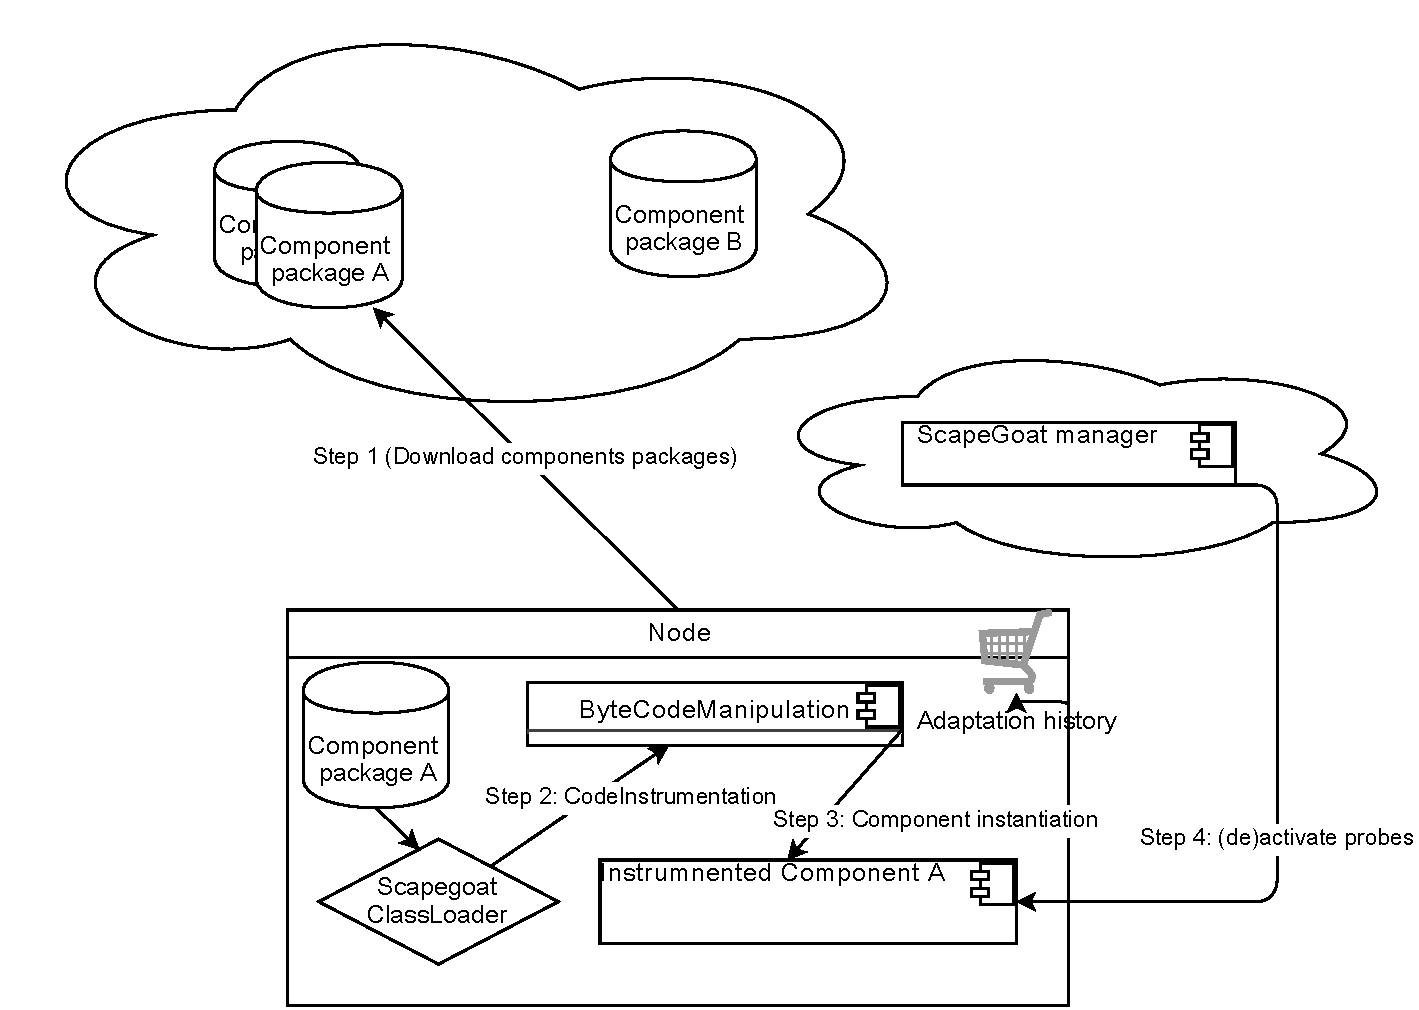
\includegraphics[scale=0.4]{figures/approach}
%	\caption{\label{fig:approach}Approach overview}
%	\end{figure}


\subsubsection{Scapegoat's architecture}

The Scapegoat framework is built using the Kevoree component framework.
Scapegoat extends Kevoree by providing a new Node Type and three new Component Types:
\begin{itemize}
\leftskip -.2in
\item \textbf{Monitored Node.}
Handles the admission of new components by storing information about resource availability.
Before admission, it checks the security policies and registers components with a contract in the monitoring framework.
Moreover, it intercepts and wraps class loading mechanisms to record a component type's loaded classes.
Such information is used later to (de)activate the probes.
\item \textbf{Monitoring Component.}
This component type is in charge of checking component contracts. 
Basically, it implements a complex variant of the algorithm in Listing \ref{algo:monitoring}.
It communicates with other components to identify suspected components.
% and to adapt the system after a fault is identified.
%todo: WHAT DOES THIS MEAN? Additionally, it makes use of another software artifact to deal with the (de)activation of probes. 
\item \textbf{Ranking Component.}
This is an abstract Component Type; therefore it is user customizable.
It is in charge of implementing the heuristic that ranks the components from the most likely to be faulty to the least likely.
\item \textbf{Adaptation component.}
This component type is in charge of dealing with the adaptation of the application when a contract violation is detected.
It is also a customizable component.
The adaptation strategy whenever a faulty component is discovered is out os scope of this thesis.
Nevertheless, several strategies may be implemented in Scapegoat, such as removing faulty components or slowing down communication between components when the failure is due to a violation in the way one component is using another.
\end{itemize}

\subsubsection{Extensibility of the Scapegoat Framework}
%\todo{For Walter: Review this section}
%\todo{We need to talk about three things: the heuristics, the admission control and the contracts semantics or implementation extensibility}

The Scapegoat framework has been built with the idea of being as generic as possible, thus supporting various extensions and specializations.
In this section we discuss the extension points provided by the Scapegoat framework.

%Defining heuristics to rank components is a part of the framework that can be specialized 
Heuristics used to rank suspected faulty components can be highly specialized
and, as we show in section~\ref{sec:evaluation}, have a remarkable impact on the behavior of Scapegoat.
A new heuristic is created by defining a component that implements an interface to provide a ranking of the suspected components.
To do so, a context is sent with each ranking request on this component.
This context is composed of three elements, 
i) a model that describes the components and links of the deployed application, 
%ii) a models' history which contains all the models that have been deployed on the platform, and 
ii) a history that contains all the models that have been deployed on the platform, and 
iii) a history of failures composed of metadata regarding what components have failed as well as why and when it happened.
In this thesis, we present three heuristics.
The first heuristic is proposed in section~\ref{sec:heuristic-based-on-modeling} and shows how we can leverage the Models@Run.time paradigm to guide the framework in finding the component that is behaving abnormally.
Due to their simplicity, the other two heuristics are presented in section~\ref{sec:evaluation} where we use them to evaluate the behavior of Scapegoat.

The mechanism for creating new heuristics is based on the strategy design pattern. Figures \ref{fig:strategy-class} and \ref{fig:strategy-sequence} illustrates this extension point. 


\begin{figure}[h!]
\centering
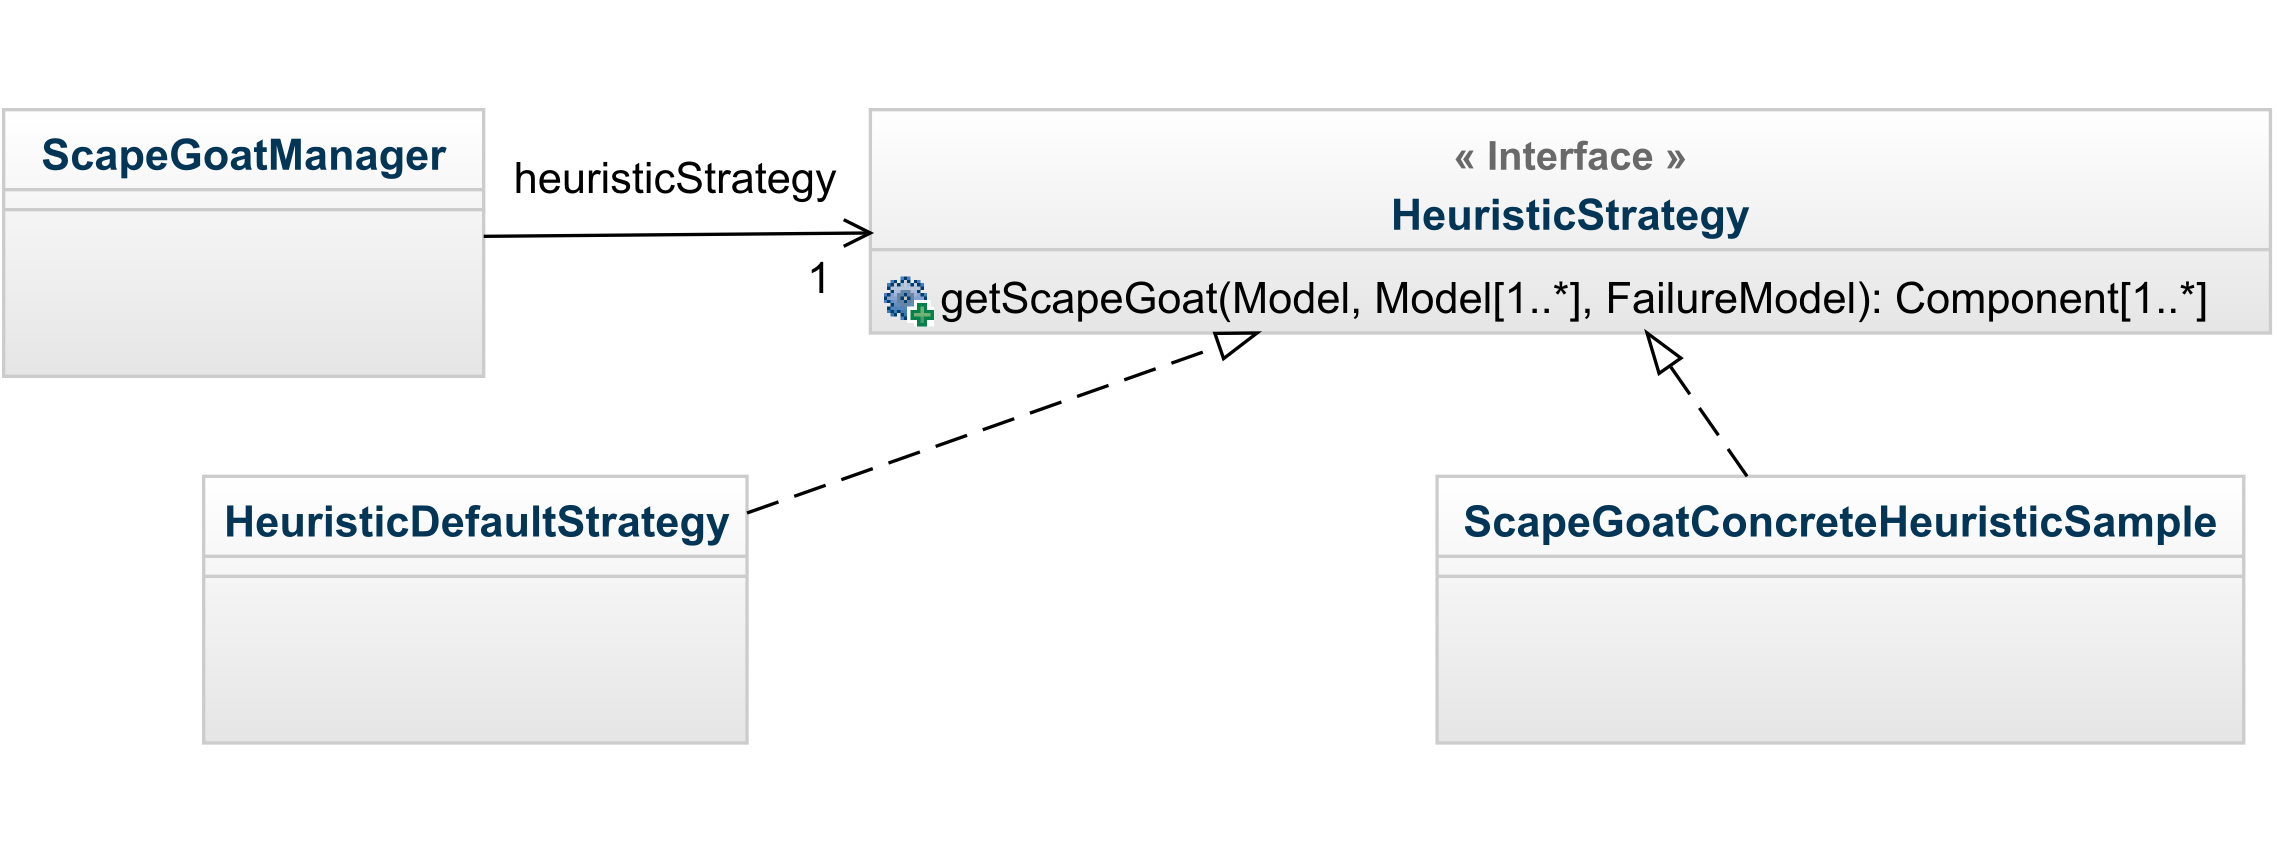
\includegraphics[width=0.9\textwidth]{./chapter5/figures/strategy-class}
\caption{\label{fig:strategy-class}Heuristic extension point in Scapegoat. This illustrates the class diagram.}
\end{figure}

\begin{figure}[h!]
\centering
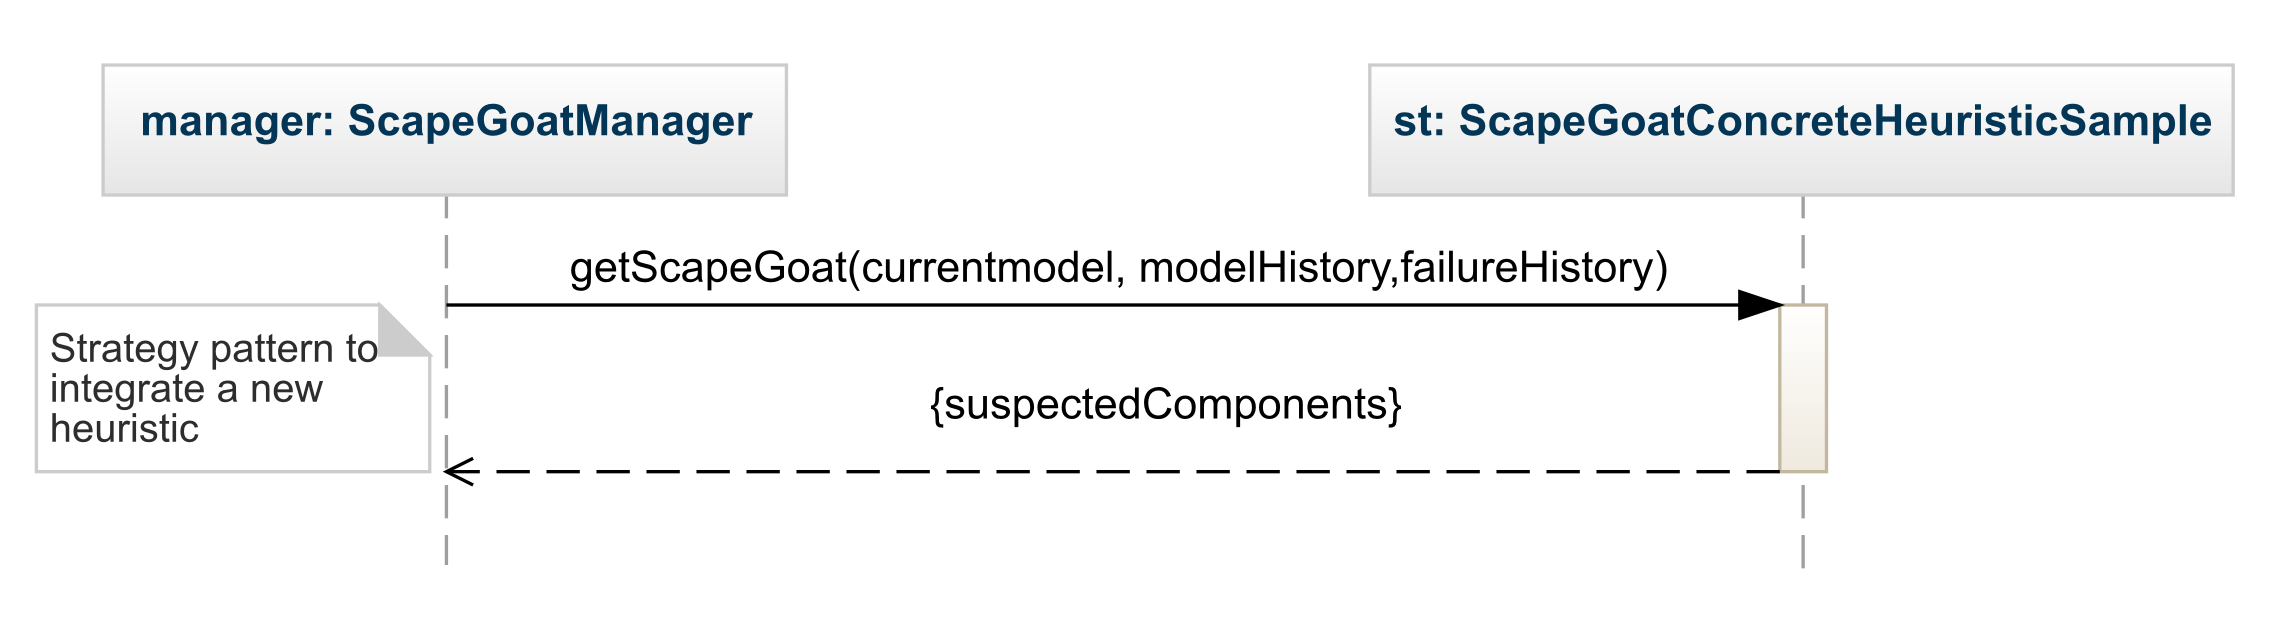
\includegraphics[width=0.9\textwidth]{./chapter5/figures/strategy-sequence}
\caption{\label{fig:strategy-sequence}A sequence diagram showing how the extension point to define heuristics in Scapegoat is used.}
\end{figure}

A second extensible aspect of the framework is the admission control system.
The framework provides an API to hook user-defined actions when new components are submitted for deployment.
Basic data describing the execution platform in terms of resource availability, information about the already deployed components and the new component's contract are sent to the user-defined admission control system.
On each request, the admission control system has to accept or refuse the new component.
We are using an approach that checks the theoretical availability of resources whenever a component is deployed, and accepts the new component if the contract can fit in the remaining available resources.
Scapegoat is meant to support other policies as, for instance, overcommitment.
 
A last element that can be specialized to user needs is the contracts semantic.
In section~\ref{componentcontract} we describe how we interpret the contract in this work.
However, it is possible to define other contract semantics, for instance, accepting values that are closed to the limit defined in the contract, or using fuzzy values instead of sharp values.
It is worth noting that modifying the semantic of the contract would likely involved redefining the domain-specific language to describe contract and also modifying the admission control system.
 
%There are many customizable features in the framework.
%Other aspects to modify are the admission control algorithm used and the logic to check if a component behaves according its contract.
%Users of the framework can also redefine the mechanism to monitor communication among components, as we do in section~\ref{sec:WebStudy}, in order to fully capture communication based on other channels.
%Finally, in a solution that really support reconfiguration, it is essential to provide adaptation strategies.


\subsubsection{Implementation strategy}
Scapegoat aims at minimizing monitoring overhead when the framework is monitoring the global behavior of the JVM. 
To achieve this, Scapegoat uses as few probes as possible when executing in global monitoring mode.
Only when it is necessary, the framework activates the required probes.
This features are implemented in the framework in three modules that are in charge of different concerns: a module to activate/deactivate the probes, a module to collect the resource usage, and a module to compute what components should be carefully monitored.
In this section we focus on the modules for activating/deactivating probes and for collecting information of resource usage because they required considerable engineering effort.
Notice, however, that this module is executed on demand when the framework already decides the monitoring mode to use and what components to monitor.

\paragraph{Module to activate/deactivate probes}
In Scapegoat  we use bytecode instrumentation to perform localized monitoring.
However, instead of doing as previous approaches that manipulate the bytecode that defines components just when the component's code is executed for the first time, we modify the bytecode many times during components' life.
Every time the monitoring mode is changed we either activate or deactivate the probes by simply inserting them in the bytecode or by removing them. 
Implementing this mechanism at per-component basis requires knowing all the classes that have been loaded for a component.
This information is kept using a dictionary in which we treat a component's id as a key and a set of class names as a value.
The dictionary is filled using the \textit{traditional} classloader mechanism of Java.
In short, when a class is loaded on behalf of a component, we detect the class name and the thread that is loading the class.
Using the thread's id we are able to identify the component because we use special naming conventions for each thread executing the initial code of a component.
When probes are activated/deactivated on a component, iterating over the set of class names allows the re-instrumentation of each involved class.

The probes perform two actions: collecting data about the local usage of resources (e.g., objects recently allocated, instructions executed in the current basic block, bytes sent through the network), and notifying to the resource consumption monitor about the collected data. 
Some data we collect is computed statically when the bytecode is loaded.
This includes the size of each basic block and the size of each object allocated when the size of each instance of the class is already known.
Other data, such as bytes sent through the network or the size of allocated arrays, can only by collected dynamically when the code is running.
To notify about the collected data we use simple method calls to a proxy class in charge of forwarding the data to the monitoring module.
Probes to detect CPU consumption are inserted at the end of each basic block.
These probes collect the size in number of instructions of its container basic block.
Probes for IO throughput and network bandwidth are added in a few selected method defined in classes of the Java Development Kit (JDK).
These probes take the needed information from local variables (e.g., number of bytes) and call the proxy class. 

Our implementation, which is built using the ASM library~\footnote{asm.ow2.org} for bytecode manipulation and a Java agent to get access to and transform the classes, is based on previous approaches to deal with resource accounting and profiling in Java~\cite{binder_portable_2006,Binder200645,czajkowski_jres:_1998}.
As in previous approaches, we compute the length of each basic block to count the number of executed instructions and we try to keep a cache of \textit{known} methods with a single basic block.
Moreover, we compute the size of each object once it is allocated and we use \textit{weak} references instead of \textit{finalizers} to deal with deallocation.

\paragraph{Module to collect information regarding resource usage}
In Scapegoat, there are two mechanisms to collect information about how components consume resources.

The first mechanism is able to capture the usage of CPU, IO throughput, network bandwidth and memory.
Every time a probe that was inserted in the code of a component is executed, the proxy class forwards the local resource usage to the module in charge of collecting the resource usage.
Along with the local resource usage, probes also notify the id of the components consuming resource.
Such data is then used to aggregate the global consumption of each component.
It is worth noting that, when this first mechanism is used to collect memory consumption, on object is always accounted as  consumed for the component responsible for its initial allocation.
In short, no matter whether the initial component $C$ that allocates the object no longer held a reference to an object $O$, as long as $O$ remains in memory, $C$ is accounted for its consumption.
Moreover, as was already mentioned, using this mechanism is not possible to deactivate the probes related to memory consumption.

On the contrary, the second mechanism is only useful to collect information about memory consumption.
The advantages of this method are: we can leverage the proposed optimistic monitoring because it executes only on demand, and it has no impact on the number of objects allocated in memory because no \textit{weak references} are used.
However, in this method an object $O$ is consumed not for the component that allocates it but for those components that held references to it.
As a consequence, in certain occasions the framework states that an object is being consumed for many components at the same time. 
We built this solution on top of JVMTI by implementing the algorithm proposed in~\cite{Price:2003:GCM:829515.830545, dsn/09/geoffray/ijvm}, with the main difference being that our solution works without modifying the garbage collector.
In summary, this algorithm simply try to find those objects that are reachable from the references of each component.
It does so by traversing the graph of live object using as the component instance and its threads as roots of the traversal. 
Since our approach does not require a modification to the garbage collector, it is portable and works with different garbage collector implementations.

%\subsubsection{Quality of Contract} 

%\todo{}
%\todo{do not forget to have a part on implementation}

\subsection{Leveraging Models@run.time to build an efficient monitoring framework}\label{sec:heuristic-based-on-modeling}
As presented in section \ref{monitorContainer}, our approach offers a dynamic way to activate and deactivate fine-grain localized monitoring.
We use a heuristic to determine which components are more likely to be faulty.
Suspected components are the first to be monitored.

%\hl{Isn't this a conclusion of the evaluation? Why is it here?}
%When compared to fine-grain monitoring of all components, our technique decreases the accumulated overhead of the monitoring system when a problem is detected.
%It should be noted that a poorly performing heuristic may introduce extensive delays in identifying faulty components.
%With this in mind, our approach is a trade-off between low monitoring overhead and the delay introduced to identify the faulty component (i.e., overhead versus latency).
%Thus, the overall performance of our approach is tightly coupled to the performance of our heuristic in accurately finding faulty components.

Our framework supports the definition of different heuristics, which can be application or domain-specific.
In this chapter we propose a heuristic that leverages the use of the Models@run.time approach to infer the faulty components.
The heuristic is based on the assumption that the cause of newly detected misbehavior in an application is likely to come from the most recent changes in the application.
This can be better understood as follows:
\begin{itemize}
\leftskip -.2in
  \item recently added or updated components are more likely to be the source of a faulty behaviour;
  \item components that directly interact with recently added or updated components are also suspected.
\end{itemize}

We argue that when a problem is detected it is probable that recent changes have led to this problem, or else, it would have likely occurred earlier.
If recently changed components are monitored and determined to be healthy, it is probable that the problem comes from direct interactions with those components.
Indeed, changes to interactions can reveal dormant issues with the components.
The algorithm used for ranking the components is presented in more detail in Listing \ref{algo:heuristic}.
%todo: WHAT???? Note that in this heuristic, each subset of components to be finely monitored is composed for one element of the list.
In practice, we leverage the architectural-based history of evolutions of the application, which is provided by the Models@run.time approach.
%The heuristic starts at the most recently changed components, because they are more likely to have introduced the problem, and we iteratively move to older components.


\begin{lstlisting}[escapeinside={(*}{*)},caption=The ranking algorithm (uses the model history for ranking).,label=algo:heuristic,float=!h]
ranker() : list<Component>
	// used to avoid adding duplicated elements to the list
	visited = (*$\emptyset$*)
	// this list will contain the result of calling the routine
	ranking = {}
	for each model M (*$\in$*) History
		// adding components that were added in this model
		N = {c (*$\mid$*) c was added in M}
		ranking.add N(*$\setminus$*)visited
		visited = visited (*$\cup$*) N
		// finding neighbors
		Neighbors (*$ = \bigcup_{c \in N}{c.neighbors}$*)
		SortedNeighbors = sort (Neighbors (*$\setminus$*) visited, History)
		// adding neighbors
		ranking.add SortedNeighbors
		visited = visited (*$\cup$*) Neighbors
	// return the built ranking
	return ranking

// this routine recursively sort a set of components using the following criteria:
// components are sorted by the timestamp that indicates when they were installed
private sort (S : Set<Component>, H : History) : list<Component>
	r = {}
	if (*$S \ne \emptyset$*)
		choose (*$b \mid b \in S$*) (*$\wedge$*) b is newer with respect to H than any other element in S
		r.add b, sort (S(*$\setminus$*){b}, H)
	return r
\end{lstlisting}

Listing~\ref{algo:heuristic} shows two routines, but only routine \textit{ranker} is public.
It can be called by the monitoring system when it is necessary to figure out in what order components must be carefully monitored. 
After initializing an empty list which will hold the rank, the algorithm starts to iterate in line 6 over the history of models that have been installed in the system.
As mentioned, this history contains a sorted set of models that describe what components have been installed in the system.
Within each iteration, the algorithm first computes in line 8 the set of components that were installed at such a point in time.
Afterwards, these components are added to the result.
The next step, executed at lines 12 and 13, is finding those components that are directly connected to components that were added to the application at this point in time.
Finally, these \textit{neighbors} are added to the rank after being sorted.
Routine \textit{sort} simply sorts a set of components using as criteria the time at which components where installed in the system.

%We implemented this alogrithm using the kevoree framework that provide the model to know the interactions between components and which offer access to the model history.
%\subsection{Analysis of expected behaviour}\label{analysis}
%
During adaptive monitoring, the monitoring system transits between either \textit{Global} lightweight monitoring (G) and \textit{All Components} or full monitoring (F), or Global and \textit{Specific} monitoring based on heuristics (H).
We can describe the transitions back and forth as:
\begin{subequations}
\begin{align}
G \rightarrow F \label{tA1}
\\F \rightarrow G \label{tA2}
\end{align}
\end{subequations}
\begin{subequations}
\begin{align}
G \rightarrow H \label{tH1}
\\ H \rightarrow G \label{tH2}
\end{align}
\end{subequations}
Different monitoring modes have different times to detect a failure.
We denote by $T_{df}(F),T_{df}(G),T_{df}(M_x)$ the time to detect failure of full, global and subset monitoring respectively. 
We know by construction that relations \eqref{dt0}, \eqref{dt1} and \eqref{dt2} hold.
This means that full monitoring should detect both the existence of a fault and the source of a fault faster than adaptive monitoring because all components are continuously checked instead of just a lightweight global check\footnote{It should be noted that the lightweight global monitoring mode can only detect the existence of a fault but not the source of the fault. To detect the source of the fault, more intrusive, per-component monitoring is required}.
However, there is no direct relationship between the two variants of adaptive monitoring (i.e., \eqref{dt1} and \eqref{dt2}) because the delay depends on the time needed to probe and instrument components (varies according to the number and size of classes), and the quality of the heuristic in targeting faulty components as quickly as possible.
The former element affects the delay when \textit{all components} are instrumented.
The latter depends on the ability of the heuristic to include the faulty component inside the set of suspected faulty components.
\begin{subequations}
\begin{align}
T_{df}(F) \le T_{df}(G) \label{dt0}
\\ T_{df}(F) \le T_{df}(G) + \sum_{i=0}^{j}(T_{trans}(C_i) + T_{df}(M_i)) \label{dt1}
\\ T_{df}(F) \le T_{df}(G) + T_{trans}(all) + T_{df}(M_{all}) \label{dt2}
\end{align}
\end{subequations}
%The experiments have shown the impact of monitoring policies over performance.
Another important dimension is the global overhead of each policy on the running system.
The following relations apply to this dimension.
Relation \eqref{overheadRelations1} is true because Full monitoring is always costlier than lightweight Global monitoring.
Relations \eqref{overheadRelations2} and \eqref{overheadRelations3} are true if a single faulty behaviour occurs during the execution of the application.
However, these relations do not apply when the number of failures and the number of transitions grow.
It is also impossible to establish a relation between the two adaptive monitoring policies because, once again, it depends on the size of the application and the quality of the heuristic in quickly finding the source of faults. 
\begin{subequations}
\begin{align} 
 O(F) > O(G) \label{overheadRelations1}
\\ O(F) > O(G) + O_{trans}(all) + O(M_{all}) \label{overheadRelations2}
\\ O(F) > O(G) + \sum_{i=0}^{j}(O_{trans}(C_i) + O(M_i)) \label{overheadRelations3}
\end{align}
\end{subequations}
Only relationship \eqref{overheadRelations1} is independent of the application.
The other relationships depend on time.
We can express overhead as a time dependent function.
For instance, let $O_F(t)$,  $O_A(t)$ be the overhead in the application due to Full monitoring and Adaptive monitoring with all components respectively.
Where: 
\begin{equation*}
O_F(t)\approx const
\end{equation*}
\begin{equation*} 
O_A(t) = 
	\begin{cases}
   		O(G) & \text{if in G state} \\
   		O_{trans}(all) & \text{if changing state in t} \\
   		O(M_{all})=O(F) & \text{if in A state}
  	\end{cases} 
\end{equation*}
The integral expresses the overhead in a given amount of time.
The relation \eqref{eq:overhead-time} is true under two conditions.
On the one hand, if time spent in global monitoring is bigger than time spent in other states.
On the other hand, if the overhead due to transitions is small.
A similar analysis is applicable to adaptive monitoring based on heuristics.
\begin{equation}
\int O_F(t)\,dt > \int O_A(t)\,dt \label{eq:overhead-time}
\end{equation}
The first condition is reasonably met through the two following factors.
First, we can expect that most applications have few failures in comparison to the global execution time of the application.
Second, the application container should provide an adaptation mechanism to remove the source of failure when a contract violation is identified.
This adaptation would allow the system to transition back into global monitoring.

Following the previous analysis we can conclude that the overhead of the monitoring framework depends on the following factors: the time spent in global monitoring, the number of transitions performed to intrusive monitoring, the quality of the heuristic, and the size of the application.
Likewise, the quality of the heuristic and the size of the application affect the delay to detect failures.
%We can now see that the behavior of \textit{all monitoring} strategy is due to the hostile execution environment we are using.
%The behavior change completely if we introduce an adaptation mechanism to remove the faulty component instead of allowing the its uncontrolled execution.



\section{ScapeGoat Performance Evaluation\label{sec:evaluation}}
In this section we present a first series of experiments and discuss the usability of our approach.
We focus on the following research questions to assess the quality and the efficiency of ScapeGoat:

\begin{itemize}
	\item \textbf{What is the impact of the various levels of instrumentation on the application?}
	Our approach assumes high overhead for full monitoring and low overhead for a lightweight global monitoring system. The experiments presented in section \ref{sec:OverheadFullMonitoring} show the overhead for each instrumentation level.
	\item \textbf{What is the performance cost of using instrumentation-based and heap-exploration-based memory monitoring?}
	Since both mechanisms have by design different features, the experiments in section \ref{sec:OverheadFullMonitoring} show the overhead each mechanism produces. 
	\item \textbf{Does our adaptive monitoring approach have better performance than state-of-the-art monitoring solutions?}
	The experiment presented in section \ref{sec:adaptive-vs-full} highlights the performances benefits of our approach considering a real-world scenario.
	\item \textbf{What is the impact of using a heuristic in our adaptive monitoring approach?}
	The experiment presented in section \ref{sec:switch-heuristic} highlights the impact of the application and component sizes, and the need of a good heuristic to quickly identify faulty components.
%Our last experiments aims at showing the potential benefits of the Heuristics in our approach. The experiment presented in section \ref{heuristic_eval} highlights the benefits of using a heuristics with a growing size of the application.
\end{itemize}

The efficiency of our monitoring solution is evaluated on two dimensions: the overhead on the system and the delay to detect failures.
We show there is a trade-off between the two dimensions and that ScapeGoat provides a valuable solution that increases the delay to detect a faulty component but reduces accumulated overhead.
This evaluation has been conducted on a Cyber Physical System case study.
It corresponds to a concrete application that leverage the Kevoree framework for dyamic adaptation purpose.

We have built several use cases based on a template application from our motivating example in section \ref{sec:scapegoat-motivaing-example}.
We reused an open-source crisis-management application for firefighters that has been built with Kevoree components.
We use two functionalities of the crisis-management application.
The first one is for managing firefighters.
The equipment given to each firefighter contains a set of sensors that provides data for the firefighter's current location, his heartbeat, his body temperature, his acceleration movements, the environmental temperature, and the concentration of toxic gases. 
These data are collected and displayed in the crisis-management application, which provides a global-view of the situation. 
The second functionality uses drones to capture real-time video from an advantageous point-of-view.

Figure \ref{fig:complete-usecase} shows the set of components that are involved in our use-case, including components for firefighters, drones and the crisis-management application\footnote{More information about these components is given in \url{http://goo.gl/x64wHG}}. The components in the crisis-management application are used in our experiments, but the physical devices (drones and sensors) are simulated through the use of mock components.
The application presents two components: the first one is a web browser that shows information about each firefighter in the terrain, and the second one allows to watch the video being recorded by any drone in the field.
A Redis database is used to store the data that is consumed for the application's GUI.

\begin{figure*}[!bt]
	\centering
	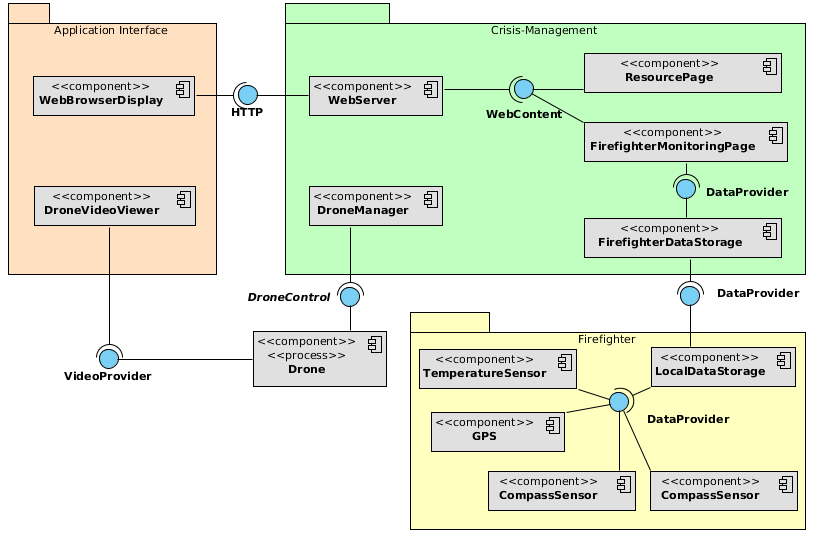
\includegraphics[scale=0.4]{./chapter5/figures/complete-usecase-new2}
	\caption{\label{fig:complete-usecase}The component configuration for our crisis-management use-case.}
\end{figure*}

Every use case we present extends the crisis-management base application by any one of the following possibilities: adding new or redundant components, adding external Java applications with wrapper components (e.g., Weka, DaCapo), or modifying existing components (e.g., to introduce a fault into them).
Using this template in the experiments allow us to measure the behavior of our proposal in a more realistic environment where many components with different features co-exist.
%is extended in every use case by: modifying existent components (e.g, to introduce faulty behavior), adding new redundant components and adding external java applications with a wrapper component.
%The particular features of each component are details in each experiment.

\subsection{Measurement Methodology} \label{sec:measurement_metodology}
To obtain comparable and reproducible results, we used the same hardware across all experiments: a laptop with a 2.90GHz Intel(R) i7-3520M processor, running Fedora 19 with a 64 bit kernel and 8GiB of system memory.
We used the HotSpot Java Virtual Machine version 1.7.0\_67, and Kevoree framework version 5.0.1.
Each measurement presented in the experiment is the average of ten different runs under the same conditions. 
%In addition to the template application we presented, we introduce a new component to execute an external jar file. This new component is used to measure the impact of the faulty behavior on the execution of the system by measuring its execution time.

The evaluation of our approach is tightly coupled with the quality of the resource consumption contracts attached to each component.
We built the contracts following classic profiling techniques. 
The contracts were built by performing several runs of our use cases, without inserting any faulty components into the execution.
Firstly, we executed the use cases in an environment with global monitoring activated to get information for the global contract.
Secondly, per-component contracts were created by running the use cases in an environment with full monitoring.

\subsection{Overhead of the instrumentation solution\label{sec:OverheadFullMonitoring}}
Our first experiment compares the various instrumentation levels to show the overhead of each one. 
In this section, \emph{Memory instrumentation} refers to the technique for accounting memory which leverage bytecode instrumentation, while \textit{Heap Exploration} refers to the memory accouting technique which leverage on-demand heap exploration.
%The results of the evaluation are fundamental because they justify the interest of our adaptative monitoring approach. 
%Additionally, these results are the baseline to understand the rest of the evaluation. 
In this experiment, we compare the following instrumentation levels: \emph{No monitoring}, \emph{Global monitoring}, \emph{Memory instrumentation}, \emph{Instructions instrumentation}, \emph{Memory and instructions instrumentation} (i.e., Full monitoring).
We also evaluate the impact on performance of the two fine-grain memory monitoring approaches we proposed: instrumentation-based and heap-dump-based.

In this set of experiments we used the DaCapo 2006 benchmark suite \cite{Blackburn:2006:DBJ:1167473.1167488}. 
We developed a Kevoree component to execute this benchmark~\footnote{\url{http://goo.gl/V5T6De}}.
The container was configured to use full monitoring and the parameters in the contract are upper bounds of the real consumption\footnote{Scripts are generated from those available at \url{http://goo.gl/FR8LC7}.}.

\begin{figure}[!ht]
\centering
\begin{tikzpicture}
\begin{axis}[
every axis legend/.append style={nodes={right}},
ybar=0pt,
legend style={at={(0.25,1.1)},
anchor=north,legend columns=1, font=\tiny},
ylabel={Time (seconds)},
y label style={at={(0.04, 0.5)}},
scaled y ticks = false,
      y tick label style={/pgf/number format/fixed,
      /pgf/number format/1000 sep = \thinspace % Optional if you want to replace comma as the 1000 separator 
      },
xtick=data,ymin=0,
width = 13cm,
height = 5cm,
bar width = 6,
x tick label style={rotate=45,anchor=east, font=\small},
 axis lines*=left, % Don't display the top and right lines
 symbolic x coords={antlr,fop,hsqldb,jython,chart,luindex,xalan,lusearch}
]
\addplot[fill=black] coordinates 
	{(antlr,1.28) (fop,1.101) (hsqldb,2.337) (jython,2.351) (chart,2.534) (luindex,3.561) (xalan,1.224) (lusearch,1.305)};
\addplot[fill=gray] coordinates 
	{(antlr,1.023) (fop,1.039) (hsqldb,2.284) (jython,2.524) (chart,2.417) (luindex,3.165) (xalan,1.191) (lusearch,1.321)};
\addplot[pattern=north east lines] coordinates 
	{(antlr,2.164) (fop,1.188) (hsqldb,8.655) (jython,10.688) (chart,4.806) (luindex,8.001) (xalan,4.885) (lusearch,9.349)};
\addplot[pattern=crosshatch] coordinates 
	{(antlr,6.235) (fop,1.905) (hsqldb,9.091) (jython,10.905) (chart,8.985) (luindex,44.988) (xalan,8.026) (lusearch,9.261)};
\addplot[pattern=dots] coordinates 
	{(antlr,7.468) (fop,1.970) (hsqldb,15.888) (jython,18.625) (chart,11.502) (luindex,51.660) (xalan,11.188) (lusearch,18.975)};
\legend{No monitoring, Global monitoring, Memory instrumentation,Instructions instrumentation, Memory \& Instructions instrumentation}
\end{axis}
\end{tikzpicture}
\caption{Execution time for tests using the DaCapo Benchmark\label{overhead-of-monitoring}}
\end{figure}

Figure \ref{overhead-of-monitoring} shows the execution time of several DaCapo tests under different scenarios when only instrumentation is used to provide fine-grain monitoring.
First, we wish to highlight that \emph{Global monitoring} introduces no overhead compared with the \emph{No monitoring} mode.
Second, the overhead due to memory accounting is lower than the overhead due to instruction accounting.
This is very important because, as we described in section \ref{monitorContainer}, memory probes cannot be deactivated dynamically.

To perform the comparison, we evaluate the overhead produced for each monitoring mode. We calculated the overhead as: \[overhead=\frac{WithInstrumentation}{GlobalMonitoring}\]

The average overhead due to instruction accounting is 5.62, while the value for memory accounting depends on the monitoring mechanism.
If bytecode instrumentation is used, the average overhead is 3.29 which is close to the values reported in \cite{Binder:2009:PPV:1464245.1464249}.
In the case of instruction accounting, these values are not as good as the values reported in \cite{Binder:2009:PPV:1464245.1464249}; because they obtain a better value between 3.2 and 4.3 for instructions accounting.
The performance difference comes from a specific optimization that we chose not to apply.
The optimization provides fast access to the execution context by adding a new parameter to each method.
Nevertheless, this solution needs to keep a version of the method without the new parameter because native calls cannot be instrumented like that. 
We decided to avoid such an optimization because duplication of methods increases the size of the applications, and with it, the memory used by the heap.
In short, our solution can reach similar values if we include the mentioned optimization, but at the cost of using more memory.
On the other hand, the values we report are far lower than the values reported in \cite{Binder:2009:PPV:1464245.1464249} for hprof.
Hence, we consider that our solution is comparable to state of the art approaches in the literature.

In Figure~\ref{overhead-of-monitoring-with_heapexplorer} we compare the execution time of the same benchmarks but using different memory monitoring approaches.
This comparison is important because, as explained in section~\ref{monitorContainer}, the two approaches have different CPU footprint.
These are controlled experiments where, in order to stress the technique, we demand the execution of a \textit{heap exploration} step every two seconds, which is not the expected usage pattern.
On the contrary, the memory instrumentation technique is executed with the expected usage pattern.
In comparison to using memory instrumentation where the average execution time is 3.29, the average overhead in execution time  decreases to 1.79 if the \textit{Heap Exploration} monitoring mechanism is used.
This value is better than the value reported in \cite{Binder:2009:PPV:1464245.1464249}.
These results suggest that this technique has less impact on the behavior of applications being monitored.

\begin{figure}[!ht]
\centering
\begin{tikzpicture}
\begin{axis}[
every axis legend/.append style={nodes={right}},
ybar=0pt, legend style={at={(0.25,1.1)},
anchor=north,legend columns=1, font=\tiny},
ylabel={Time (seconds)},
y label style={at={(0.04, 0.5)}},
scaled y ticks = false,
      y tick label style={/pgf/number format/fixed,
      /pgf/number format/1000 sep = \thinspace % Optional if you want to replace comma as the 1000 separator 
      },
xtick=data,ymin=0,
width = \textwidth,
height = 5cm,
bar width = 6,
x tick label style={rotate=45,anchor=east, font=\small},
 axis lines*=left, % Don't display the top and right lines
 symbolic x coords={antlr,fop,hsqldb,jython,chart,luindex,xalan,lusearch}
]
% no monitoring
\addplot[fill=black] coordinates 
	{(antlr,1.28) (fop,1.101) (hsqldb,2.337) (jython,2.351) (chart,2.534) (luindex,3.561) (xalan,1.224) (lusearch,1.305)};
% memory
\addplot[pattern=north east lines] coordinates 
	{(antlr,2.164) (fop,1.188) (hsqldb,8.655) (jython,10.688) (chart,4.806) (luindex,8.001) (xalan,4.885) (lusearch,9.349)};
% heap dump
\addplot[pattern=crosshatch dots] coordinates 
	{(antlr,1.143) (fop,1.125) (hsqldb,8.639) (jython,2.762) (chart,2.836) (luindex,3.589) (xalan,1.822) (lusearch,5.078)};
% memory and instructions
\addplot[pattern=dots] coordinates 
	{(antlr,7.468) (fop,1.970) (hsqldb,15.888) (jython,18.625) (chart,11.502) (luindex,51.660) (xalan,11.188) (lusearch,18.975)};
% heap dump and instructions
\addplot[fill=white] coordinates 
	{(antlr,6.159) (fop,1.188) (hsqldb,14.647) (jython,10.950) (chart,9.059) (luindex,44.758) (xalan,7.812) (lusearch,15.990)};
% legend
\legend{No Monitoring, Memory instrumentation, Heap Exploration, Memory \& Instructions instrumentation, Heap Exploration \& Instructions Instrumentation}
\end{axis}
\end{tikzpicture}
\caption{Comparison of execution time for tests using two different memory monitoring techniques\label{overhead-of-monitoring-with_heapexplorer}}
\end{figure}

The results of our experiment shown in Figures~\ref{overhead-of-monitoring} and~\ref{overhead-of-monitoring-with_heapexplorer} demonstrate the extensive impact of the \emph{Full monitoring} mode, which uses either \emph{Memory instrumentation} or \emph{CPU instrumentation}, has on the application. Thus, our \emph{Adaptive monitoring} mode, which uses \emph{Global monitoring} and switches to \emph{Full monitoring} or \emph{localized monitoring}, has the potential to reduce this accumulated overhead due to the fact that \emph{Global monitoring} has no appreciable overhead. 
%The results of the evaluation are fundamentals because they justify the interest of our adaptative monitoring approach. 
%Additionally, these results are the baseline to understand the rest of the evaluation. 

%In addition, we plan to study alternatives to improve instruction accounting. %These alternatives are about using peak monitoring and learning monitoring.
%For example, we plan to study the use of machine learning for monitoring \cite{tesauro2006hybrid}. Based on a machine learning approach, it is possible to train the monitoring system to do the instruction instrumentation. Then, instead of doing normal instruction instrumentation, we might only do, for example, method-calls instrumentation and with the learning data, the monitoring system should be able to infer the CPU usage of each call, whilst lowering the overhead.

\subsection{Overhead of Adaptive Monitoring vs Full Monitoring\label{sec:adaptive-vs-full}}
The previous experiment highlights the potential of using \emph{Adaptive monitoring}. However, switching from \emph{Global monitoring} to either \emph{Full} or \emph{Localized monitoring} introduces an additional overhead due to having to instrument components and activate monitoring probes.
Our second experiment compares the overhead introduced by the adaptive monitoring with the overhead of \emph{Full monitoring} as used in state-of-the-art monitoring approaches. 
%The result of this experiment shows the potential interest of the adaptive monitoring approach.

Table \ref{use-cases-sheet2} shows the tests we built for the experiment.
We developed the tests by extending the template application. Faults were introduced by modifying an existing component to break compliance with its resource consumption contract.
We reproduce each execution repetitively; thus, the faulty behaviour is triggered many times during the execution of the application. The application is not restarted.
%\hl{We selected as heuristic in almost every case \textit{number-of-failures} which is the best because there is only a single faulty component.}\todo{must be explain later}

\begin{table*}[!hb]
\centering
\caption{Features of use cases.\label{use-cases-sheet2}}
\begin{tabular}{|c|p{2.1cm}|p{1.4cm}|p{2cm}|p{2.5cm}|}
\hline Test Name & Monitored\newline Resource & Faulty\newline Resource & Heuristic & External Task \\ 
\hline UC1 & CPU, Memory & CPU & number\newline of failures & Weka, training neural network \\ 
\hline UC2 & CPU, Memory & CPU & number\newline of failures & dacapo, antlr \\ 
\hline UC3 & CPU, Memory & CPU & number\newline of failures & dacapo, chart \\ 
\hline UC4 & CPU & CPU & number\newline of failures & dacapo, xalan \\ 
\hline UC5 & CPU, Memory & CPU & less number\newline of failures\newline first  & dacapo, chart \\ 
\hline UC6 & Memory & CPU & number\newline of failures & Weka, training neural network \\ 
\hline 
\end{tabular} 
\end{table*}


Figure \ref{adaptive-vs-full} shows the execution time of running the use cases with different scenarios.
Each scenario uses a specific monitoring policy (\emph{Full monitoring}, \emph{Adaptive monitoring with All Components}, \emph{Adaptive monitoring with Localized monitoring}, \emph{Global monitoring}).
All these scenarios were executed with the heap explorer memory monitoring policy. 
This Figure shows that the overhead differences between \textit{Full monitoring} and \emph{Adaptive monitoring with All Components} is clearly impacted by scenarios that cause the system to transition too frequently between a lightweight Global and a fine-grain \emph{Adaptive monitoring}.
Such is the case for use cases UC3 and UC4 because the faulty component is inserted and never removed.
%As we explained in section \ref{analysis}, 
Using \emph{Adaptive monitoring} is beneficial if the overhead of \emph{Global monitoring} plus the overhead of switching back and forth to \emph{All Components monitoring} is less than the overhead of the \emph{Full monitoring} for the same execution period.
If the application switches between monitoring modes too often then the benefits of adaptive monitoring are lost.

The overhead of switching from \emph{Global monitoring} to \emph{full components} or \emph{Localized monitoring} comes from the fact that the framework must reload and instrument classes to activate the monitoring probes.
Therefore, using \emph{Localized monitoring} reduces the number of classes that must be reloaded.
This is shown in the third use-case of Figure~\ref{adaptive-vs-full}, which uses a heuristic based on the number of failures.
Because we execute the faulty component many times, the heuristic is able to select, monitor and identify the faulty component quickly. This reduces overhead by 93\%. We use the following equation to calculate overhead:

\[ Gain=100-\frac{OurApproach-GlobalMonitoring}{FullMonitoring-GlobalMonitoring}*100 \]

We also evaluate the execution time for each use case using the instrumentation-based memory monitoring mode.
The average gain in that case is 81.49\% and, as shown in previous section, in average it behaves worse than the \textit{Heap Exploration} mechanism.
However, it is worth noting that the difference between using memory monitoring based on instrumentation and heap exploration is less remarkable than in the previous experiment.
Observe how in test UC4, using a combination of heap exploration and adaptive monitoring with all components behaves worse than using plain instrumentation-based memory monitoring.
In this particular test, activating and deactivating the monitoring probes dominate the execution time.
Alas, adding a heap exploration step right after the probes are activated, just add some extra overhead.
On the contrary, there is no additional step executed when we use instrumentation to measure the memory usage.
Apparently, what matter when the all components strategy is guiding the adaptive monitoring is the ratio among the amount of allocations performed by components and the size of those components.

\begin{figure}
\centering
\begin{tikzpicture}
\begin{axis}[
every axis legend/.append style={nodes={right}},
ybar=0pt, legend style={at={(0.8,1.2)},
anchor=north,legend columns=1, font=\tiny},
ylabel={Time (seconds)},
y label style={at={(0.02, 0.5)}},
scaled y ticks = false,
      y tick label style={/pgf/number format/fixed,
      /pgf/number format/1000 sep = \thinspace % Optional if you want to replace comma as the 1000 separator 
      },
xtick=data,ymin=0,
width = \textwidth,
height = 5cm,
bar width = 6,
x tick label style={rotate=45,anchor=east, font=\small},
 axis lines*=left, % Don't display the top and right lines
 symbolic x coords={UC1,UC2,UC3,UC4,UC5,UC6}
]
% full monitoring
\addplot[fill=black] coordinates 
	{(UC1,613.000) (UC2,46.363) (UC3,63.899) (UC4,78.324) (UC5,49.144) (UC6,132.949)};
% adaptive with all component
\addplot[fill=red, pattern=crosshatch dots] coordinates 
	{(UC1,432.744) (UC2,70.501) (UC3,198.554) (UC4,187.036) (UC5,32.340) (UC6,127.711)};
% adaptive with all component and heap dump
\addplot[fill=yellow, pattern=crosshatch] coordinates 
	{(UC1,410.790) (UC2,61.808) (UC3,95.503) (UC4,204.479) (UC5,16.864) (UC6,123.381)};
% adaptive with heuristic
\addplot[fill=green, pattern=north west lines] coordinates 
	{(UC1,176.413) (UC2,16.741) (UC3,29.461) (UC4,19.470) (UC5,27.001) (UC6,123.813)};
% adaptive with heuristic and heap dump
\addplot[fill=pink, pattern=dots] coordinates 
	{(UC1,169.467) (UC2,12.520) (UC3,16.403) (UC4,20.251) (UC5,15.110) (UC6,124.294)};
% global monitoring
\addplot[fill=cyan, pattern=north east lines] coordinates 
	{(UC1,166.759) (UC2,10.646) (UC3,14.37) (UC4,20.860) (UC5,14.77) (UC6,120.16)};
\legend{
	Full monitoring, 
	Adaptive with All Components using Memory Instrumentation, 
	Adaptive with All Components using Heap Exploration, 
	Localized monitoring using Memory Instrumentation, 
	Localized monitoring using Heap Exploration,
	Global Monitoring}
\end{axis}
\end{tikzpicture}
\caption{Execution time for some use cases under different monitoring policies.}\label{adaptive-vs-full}
\end{figure}

\subsection{Overhead from switching monitoring modes, and the need of a good heuristic\label{sec:switch-heuristic}}
As we explain in the previous experiments, even if using \emph{Localized monitoring} is able to reduce the overhead of the monitoring system, the switch between \emph{Global} and \emph{Localized monitoring} introduces additional overhead.
If this overhead is too high, the benefits of adaptive monitoring are lost.

In this experiment we show the impact of the application's size, in terms of number of components, and the impact of the component's size, in terms of number of classes, on adaptive monitoring. We also show that the choice of the heuristic to select suspected components for monitoring is important to minimize the overhead caused from repeated instrumentation and probe activation processes.

For the use case, we created two components and we introduced them into the template application separately.
Both components perform the same task, which is performing a \textit{primality test} on a random number and sending the number to another component.
However, one of the components causes 115 classes to be loaded, while the other only loads 4 classes.
%An additional component is in charge of generating random numbers to be consumed by the primality tester components.

We used the same basic scenario with a varying number of \textit{primality testing's} components and component sizes.
In this way, we were able to simulate the two dimensions of application size.
The exact settings, leading to 12 experiments, are defined by the composition of the following constraints:
\begin{itemize}
	\item $N_{comp} = \left\lbrace 4, 8, 16, 32, 64, 128 \right\rbrace$  which defines the number of components for the application
	\item $Size_{comp}=\left\lbrace 4, 115 \right\rbrace$ which defines the number of classes for a component
\end{itemize} 

With these use cases, we measured the delay to find the faulty component and the execution-time overhead caused by monitoring.
Figures \ref{fig:delay-time-115} and \ref{fig:delay-time-4} show the delay to detect the faulty component with regards to the size of the application.
In the first Figure, the component size is 115 classes, and in the second Figure, the component size is four classes.
%Figures \ref{fig:execution-time-many-115} and \ref{fig:execution-time-many-4} show the overhead of monitoring based on the execution time of the main task and according to the size of the application. In the first one, the component size is 115 classes and in the second one, the component size is four classes.

\input{./chapter5/delayTime}
\input{./chapter5/executionTimeManyComponents}

\subsubsection{Impact of the application size}
%\paragraph{Impact of the application size}
Figures \ref{fig:delay-time-4} and \ref{fig:execution-time-many-4} show the size of the application has an impact on the delay to detect faulty components, and also on the monitoring overhead.
We also calculated the time needed to find the faulty component with the \emph{All components} mode after its initialization (the time needed to switch from \emph{Global monitoring}).
This time is around 2 seconds no matter the size of the application.
That is the reason the switch from \emph{Global monitoring} to \emph{All components} has such a large effect on overhead.

These figures also show that using \emph{Localized monitoring} instead of \emph{All components} when switching from \emph{Global monitoring} helps reduce the impact of the application's size by reducing the number of components to monitor and the number of classes to instrument.
However, we also see that using a sub-optimal heuristic may have negatively impacted the delay to detect faulty components.
This can be explained by the multiple switches that the Random heuristic may often require to locate the faulty component.

\subsubsection{Impact of the component size}
%and \ref{fig:execution-time-many-115}, \ref{fig:execution-time-many-4}
In Figures \ref{fig:delay-time-115} and \ref{fig:delay-time-4} we can observe that the component size greatly impact the performance and the delay for ScapeGoat to find the faulty component. 
Similar to the explanation for the application's size, component size impacts the switch from \emph{Global monitoring} to \emph{Localized monitoring}, because of the class reloading and instrumentation.
A good heuristic drastically reduces the number of transitions; thus, it has a huge impact on the delay. 
When the components size increase, the choice of a good heuristics becomes even more important, because the cost of dynamic monitoring probes injection increase with the size of the components.
\section{Scapegoat to spot faulty components in a scalable diverse web application}\label{sec:WebStudy}
In this section, we present another application that benefits from the Scapegoat approach.
Although the general goal of spotting components that behave abnormally regarding resource consumption remains the same, with this use case we highlight the possibility of using Scapegoat 
%on a real application 
%and a specific usage of Scapegoat 
to automatically find buggy components on a scalable modular web application.
The section \ref{MdMS} presents an introduction to the application use case, while the remainder of the section deals with the experimental setup and the results.


\subsection{Use case presentation}\label{MdMS}
We are applying the Scapegoat approach to check resource consumption contracts on a web application called MdMS.\footnote{\url{https://github.com/maxleiko/mdms-ringojs}}
This application offers a web Content Management System based on the Markdown language for editing posts. 
MdMS uses a typical architecture (as shown in Figure \ref{fig:webapp}) for scalable web applications: a load-balancer connected to a set of workers (called MdMS Sosie in Figure \ref{fig:webapp}), which are themselves connected to a distributed database to retrieve the application specific content.
The worker layer of this application can be duplicated across various machines to support a growing number of clients.
The web application is currently online\footnote{\url{http://cloud.diversify-project.eu/}}. 

\begin{figure*}[!bt]
	\centering
	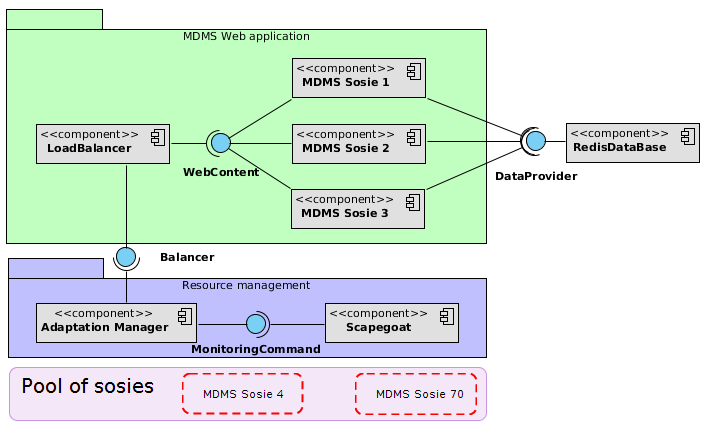
\includegraphics[scale=0.45]{./chapter5/figures/webapp2}
	\caption{\label{fig:webapp}Architecture of MdMS along with Scapegoat and additional components to adapt the system.}
\end{figure*}

The main characteristic of MdMS is that workers are not pure clones but diverse implementations of the MdMS server stack~\cite{alliermulti}.
This proactive diversification of MdMS targets safety~\cite{avizienis85} and security~\cite{Forrest97} purposes.
In particular, we have used a recent technique for the automatic synthesis of \textit{sosie} programs~\cite{baudry2014tailored} in order to automatically diversify the workers. 
A \textit{sosie} is a variant of a program that exhibits the same functionality (passes the same test suite) and a diverse computation (different control or data flow). 
\textit{Sosie} synthesis is based on the transformation of the original program through statement deletion, addition or replacement.
%The MdMS application is leveraging this diversified set of workers in order to reach the scalability property while icluding diversity in the software layer to prevent the so-called BOBE (Blow Once, Blow Everywhere) attacks~\cite{alliermulti}.

While the construction of \textit{sosies} focuses on preserving functional correctness, it ignores all the non-functional aspects of the program.
Consequently, a \textit{sosie} offers no guarantee regarding its resource consumption and may contain memory leaks or other overhead on resource consumption that can significantly impact the performance of MdMS.

In this experiment, we use Scapegoat to monitor the resource consumption of the various \textit{sosies} of the MdMS workers.
This technique enables us to identify \textit{sosies} in a production environment that do not behave according to the resource consumption contracts, allowing the system to remove these workers and use other \textit{sosies}.
Our goal in this experiment is to answer the following question:

\begin{itemize}
 \item Does Scapegoat correctly identify the faulty components in a system which includes many variants of the same component?   
\end{itemize}

\subsection{Experimental setup}

We devised this experiment as a scenario where many clients interact with the web application at the same time by adding and removing articles.
The stress produced by these requests increases the resource consumption on the server side which is running on top of Kevoree components.
Figure~\ref{fig:webapp} depicts the server side's configuration.
Since MdMS is a web application developed on top of RingoJS~\footnote{\url{https://github.com/ringo/ringojs}}, a JavaScript runtime written in Java, our \textit{sosies} include the RingoJS framework and the application that has been wrapped into Kevoree components.

In this experiment, we deploy many of these components as back-end servers of the web application and we use Scapegoat to monitor the consumption of each server.
Their contracts regarding resource consumption were built using the mechanism described in section \ref{sec:measurement_metodology} but with the original MdMS worker as a reference component.
The application also contains a component acting as a front-end that evenly distributes the requests among back-end servers.
This load balancer implements a plain round robin policy.
%There is an additional component running on the platform, it is in charge of adapting the system.
%This component reacts to events produced by Scapegoat and modifies the deployed system following the Models@run.time paradigm.

To produce a realistic load on the web server we have recorded a set of standard activities on the MdMS web site using Selenium~\footnote{\url{http://www.seleniumhq.org/}}.
We then use the Selenium facilities to replay these activities many times in parallel to provide the required work load on the server.
% of resource consumption, we generate many accesses to the system.
%We use Selenium~\footnote{http://www.seleniumhq.org/} to accomplish this purpose since MdMS is a web application.
Our experimental settings feature 120 clients which are scheduled by a pool of 7 concurrent Selenium workers.
Each client adds 10 articles to the database through the Website GUI, which represents 16 requests per article, for a total of 19200 requests to the MdMS workers sent through the load balancer.
In this experiment, the Selenium workers are executed on the same physical device as the web server, with the same testing platform described in section~\ref{sec:measurement_metodology}.

The experiment is configured as follows.
Using the diversification technique described in~\cite{baudry2014tailored}, we synthesized 20 \textit{sosies} of the MdMS workers.
These \textit{sosies} are used to execute the application with a varying number of back-ends (from 4 to 10).
One particular \textit{sosie} has been modified by hand to ensure that it violates the original component's contract.
We execute all the described components as well as the Scapegoat components on a single instance of Kevoree.

\subsection{Experimentation results}

Figure~\ref{fig:execution-time-web-app} shows the time required on the server side to reply to all the requests sent by Selenium.
Although the values might look surprisingly high at first, they are in fact the result of a heavily loaded system.
Selenium is actually rendering a couple of web pages for each added article; hence at least 2400 pages are rendered.
Moreover, both clients and servers are sharing resources because they run on the same physical device.
%Another point to highlight is that the time needed to execute all these requests remains stable when no monitoring is used and only changes abruptly when deploying ten \textit{sosies}.
%The execution times remain stable when monitoring is not activated, which is expected because the number of requests does not change between experiments, the load balancer distributes these requests evenly, and we are using the same physical device to execute all back-end servers.
%The stability of the executions when monitoring is not activated is expected because the number of requests does not change between experiments, the load balancer distributes these requests evenly, and we are using the same physical device to execute all back-end servers.
This leads to very stable execution times when monitoring is not activated because the number of requests does not change between experiments, the load balancer distributes these requests evenly, and we are using the same physical device to execute all back-end servers.
%\todo{Please, read below the explanation for: Why the execution time decreases?}
In the \textit{local monitoring} series, the global time to execute decreases until reaching 9 \textit{sosies}.
Although counterintuitive, it is caused by the effect of having \textit{localized monitoring} and \textit{load balancing} at the same time.
For instance, when four \textit{sosies} are used, the monitoring probes are periodically injected into one component out of four, hence roughly a quarter of the requests are handled by a slower \textit{sosie}.
However, with eight components the slow execution path is only taken by around 12.5\% of the requests.
The overhead of \textit{Localized monitoring} when ten \textit{sosies} are deployed increases because the physical machine reaches its limit and begins thrashing.
As a consequence, low-level interactions with the hardware (e.g. cache misses), the operating system and the JVM slow down the execution.
On average, the overhead due to monitoring with both instruction instrumentation and memory instrumentation is 1.59, which is lower than the values shown in section~\ref{sec:OverheadFullMonitoring} for full monitoring despite only one of the instrumentation mechanisms being enabled in those experiments.
The values in this section are better even if we are monitoring both resources because we are using the adaptive approach.
   

\input{./chapter5/webAppResults}

In these experiments, we evaluate the accuracy of the output and its quality in terms of the time needed to find the faulty component.
Scapegoat always spots the correct \textit{sosie}.
It does so because it is an iterative process that continues until finding the faulty component.
In addition, Scapegoat does not output false positives during these experiments.
The delay to detect faulty components is shown in Figure~\ref{fig:delay-time-web-app}.
In this case, the values remain close to 2 seconds no matter the number of \textit{sosies} used nor the execution time.
This behavior is consistent with the experiments in section~\ref{sec:evaluation} because we are also using a good heuristic for the use case.
It shows that Scapegoat can spot faulty components with an acceptable delay in a real application.

\subsection{Discussion of the use case}
This use case shows that Scapegoat is able to provide useful information in real applications.
It also highlights how the framework can help select software variants at runtime in the context of software diversity.
Or, more generally, in the field of software oriented architectures where many stakeholders may provide the same services, Scapegoat can help to choose services.
Moreover, this use case leads to a distributed usage of Scapegoat, where the policies for admission control and resource consumption monitoring can be coordinated among distributed devices.

Finally, in systems where there are many variants of the same component or service, Scapegoat provides essential information to drive application reconfiguration.
For example, the adaptation component in Figure~\ref{fig:webapp} may use Scapegoat's faulty component selection to replace a faulty \textit{sosie} or to modify the scheduling policy in the load balancer.






%\section{Related work}\label{sec:related}

The Scapegoat framework is related to component monitoring, Models@run.time, component isolation and component performance prediction approaches.

Performance and resource-consumption prediction approaches are complementary to the Scapegoat framework because they can assist in better specifying the component contracts.
Some approaches require developers to provide extensive per-component metadata at design-time in order to calculate the application's overall performance or resource consumption \cite{Becker:2007:MPP:1216993.1217006,Jonge03scenario-basedprediction}.
Prediction approaches have been achieved by using combinations of design-time and runtime analyses \cite{autili2012hybrid}.
However, although many approaches to performance prediction have been proposed, none of them have obtained widespread use \cite{Koziolek:2006:QDD:2171366.2171393}.

%In \cite{Ghezzi2009}, the authors propose using performance models based on Queuing Networks to cope with the problem of architectural reasoning.
%The authors keep Models@run.time to enable re-estimation of model parameters based on the behavior of the running system and they present a mechanism to update the parameters when usage profiles change.
%The authors target the same problem we are dealing with, although we are not facing the prediction of behavior.

KAMI \cite{Ghezzi2009} builds performance models at design-time but uses and continually refines them at runtime.
By collecting runtime data, they are able to build performance and resource consumption models that reflect real usage.
They are able to adapt the application according to changes in components' behavior, but they do not use nor propose an adaptive monitoring system to minimize overhead.

%\todo{For Walter: Review this paragraph}
State of the art monitoring systems \cite{FrenotS04,KregerHaroldWilliamson03,Binder200645} extract steady data-flows of system parameters, such as, the time spent executing a component, the amount of I/O and memory used, and the number of calls to a component.
The overhead that these monitoring systems introduce into applications is high, which makes it unlikely for them to be used in production systems.
Maurel et al. \cite{Maurel:2012:AME:2304736.2304763} propose an adaptive monitoring framework for the OSGi platform.
Similar to our approach, they propose a global monitoring system that changes to a localized monitoring system when a problem is detected.
However, their work is focused on CPU usage and does not consider other resources, such as memory or I/O.
Exploring the Java heap to obtain useful information about resource consumption has been proposed in~\cite{Price:2003:GCM:829515.830545, Geoffray5270296}.
As in our work, they account objects to the resource principal being explored (in their case to OSGi bundles) the first time an object is reached.
Their solutions modify the garbage collector in order to reduce overhead, but this causes resource accounting to be tied to, and performed on, each collection cycle.
%but it means that the accounting step is performed on each collection cycle.
In contrast, our approach can be executed on demand, albeit at the cost of further passes over the heap.
%although our accounting step requires further passes over the heap, we can precisely specify when to execute it.

Gama and Donsez \cite{Gama:2010:SCS:2176905.2176915} propose using virtual machines in separate processes or using MVM isolates \cite{czajkowski2012multitasking} to manage trusted and untrusted components.
After an evaluation period, untrusted components can be moved to the trusted JVM if no problems are detected.
This allows the main application to depend on potentially faulty components without risking severe crashes.
We can also cite Microsoft technologies such as COM (Component Object Model) components which can be either loaded in the client application process or provided in an isolated process \cite{lowy2001and}.
In addition to process virtualization, some operating systems also propose user-space virtualization, which isolates not only the processes but also the memory, the network interface and the file system. Examples of these approaches are Jails\footnote{\url{http://www.freebsd.org/doc/handbook/jails.html}} for BSD, LXC\footnote{\url{http://lxc.sourceforge.net/}} and CGroups for Linux, and lmctfy\footnote{\url{https://github.com/google/lmctfy}}.
All of these approaches have the drawback of limiting code and instance sharing and introduce additional overhead in cross-boundary component interactions.
Furthermore, depending on the complexity of the approach, there is also overhead in having to manage multiple processes.

\section{Conclusions}\label{sec:conclusion}
In this chapter we presented Scapegoat, an adaptive monitoring framework to perform lightweight yet efficient monitoring of Component-Based Systems.
In Scapegoat, each component is augmented with a contract that specifies its resource usage, such as peak CPU and memory consumption.
Scapegoat uses a global monitoring mode that has low overhead on the system, and an on-demand fine-grained localized monitoring mode that performs extensive checking of the components' contracts.
The system switches from the global monitoring mode to the localized monitoring mode whenever a problem is detected at the global level in order to identify the faulty component.
Furthermore, we proposed a heuristic that leverages information produced by the Models@run.time approach to quickly predict the faulty components. 

Scapegoat has been implemented on top of the Kevoree component framework which uses the Models@run.time approach to tame the complexity of distributed dynamic adaptations.
The evaluation of Scapegoat shows that the monitoring system's overhead is reduced by up to 92.98\% in comparison with state-of-the-art full monitoring systems. 
The evaluation also presents the benefits of using a heuristic to predict the faulty component.
In our second part of the evaluation, we highlighted the benefit of scapegoat on a classical web server architecture to dynamically determine faulty components.
This second example also exposes the capacity of Scapegoat to be applied to different application domains and confirms its relatively low overhead on the running system.
Scapegoat contributes to the state of the art by providing a monitoring framework which adapts its overhead depending on current execution conditions and leverages the architectural information provided by Models@run.time to drive the search for the faulty component.

The approach proposed in this chapter contributes to answer two research questions that were presented in the introduction of this thesis (see Section \ref{sec:intro-challenges}).
In particular, it answers \textit{RQ1} (\textit{How can we provide portable and efficient support for resource consumption monitoring?}) by describing a monitoring framework that produces low performance overhead and is fully portable.
Likewise, our proposal partially answers \textit{RQ3} (\textit{How can we leverage the knowledge about the architecture of applications to drive
a mechanism for resource management?}) by using knowledge about the structure of applications to drive the behavior of the framework.


%\selectlanguage{english}
\chapter{Squirrel: Architecture Driven Resource Management}
\label{chp:squirrel}
\markboth{Squirrel: Architecture Driven Resource Management}{Chapter5}

%\coolphrase {
%	I still don't know
%}{Some name here}


%Resource management is critical to guarantee Quality of Service when various stakeholders share the execution environment, such as cloud or mobile environments.
%In this context, providing management techniques compatible with standard practices, such as component models, is essential.
%Resource management is often realized through monitoring techniques, while resource isolation uses virtual machines or containers (e.g., docker).
%These techniques (i) impose varying levels of overhead depending on the managed resource, and (ii) are applied at different abstraction levels, such as processes, threads or objects.
%Thus, mapping components to system-level abstractions in the presence of resource management requirements can lead to sub-optimal systems.
%
%We propose Squirrel, an approach to tune component deployment and resource management in order to reduce management overhead.
%At runtime, Squirrel uses an architectural model annotated with resource requirements to guide the mapping of components to system abstractions, providing different resource management capabilities and overhead.
%We present an implementation of Squirrel, using a Java component framework,
%and a set of experiments to validate its feasibility and overhead.
%We show that choosing the right \textit{component-to-system} mappings at deployment-time reduces performance overhead and/or memory use.

\section{Introduction}

Resource management is critical for domains where software components share an execution environment but belong to different stakeholders.
For instance, in multi-tenant systems resource management is used to guarantee safety, reliability and per-stakeholder Quality of Service (QoS).
These applications essentially require the isolation of tenants in terms of resource consumption~\cite{KrWeKo2013-icwe-MTBenchmark}.
This enables, for example, \textit{Software-as-a-Service} layers for cloud systems, allowing innovative pricing policies based on user requirements. %(e.g. user A has a \textit{premium} contract that guarantees a response time inferior to 500 ms for each request, while user B has a \textit{standard} contract that does not guarantee any response time).
Since these services are often implemented on paradigms such as component models,
the design of resource management techniques dedicated to component models is an important issue.

Component model implementations represent high level concepts, such as component instances, by means of mapping them to system-level abstractions like objects, threads, processes or virtual machines.
Each mapping has unique features in terms of performance, memory footprint, etc.
However, these mappings are often done in a once-size-fits-all manner, allowing some choices to optimize for memory use while others might, for example, improve inter-component communication.
%\hl{The mapping of components to system abstractions, which has the goal of improving some parameters of the runtime, has often been made in a homogeneous way for all components.[I DON'T UNDERSTAND?, Quiero decir que todos los componentes usan el mismo mapping, todos son representados como hilos, o todos como procesos. La parte de ``som parameters'' significa que cuanod se toma esa decision durante la implementacion del framework se hace con un objetivo como reducir el uso de memoria o facilitar la comunicacion entre componentes o garantizar un ``sandbox'' para los componentes]}
Interestingly, system abstractions offer varying resource management capabilities that differ in how they impact the application.
Although we can hard-code the resource management concern during the design of the component model, we argue that this leads to sub-optimal systems with high  overhead~\cite{binder_portable_2006,czajkowski_jres:_1998,Maurel:2012:AME:2304736.2304763} because components have different resource requirements.

% without taking into account resource management concerns, and (ii) .

To address this issue, we propose Squirrel, an approach to resource management for component models that aims at reducing overhead.
In Squirrel, the application is deployed with a model containing resource usage contracts for each component and a detailed view of the system.
These metadata are used to choose at deployment-time the best way of representing each component in terms of system abstractions.
This contrasts with the \textit{traditional} approach of binding the representation during the design of the component model and results in the final runtime representation of the system only being known after deployment.
%uses meta-data regarding the application's structure and its requirements to deploy components on system-level abstractions.



%During deployment, the information is used to automatically create a new deployment model where components are automatically mapped into abstractions that we call \textit{containers}.
%Each \textit{container} is then configured based on the components' resource contracts, ensuring resource consumption while minimizing the overhead.

In this paper we discuss an approach to resource management applicable to any component model. To validate the feasibility of our proposal, we present a reference implementation for a Java-based component model.
A set of experiments validate its feasibility and show various aspects of its overhead.
The results demonstrate that choosing the right \textit{component-to-system} mappings at deployment-time can reduce performance overhead and/or memory footprint.
%\hl{INTI: Se que esta oracion es muy general, el problema es que no estoy seguro de si poner los numeros es lo correcto pues los ejemplos son tan solo para mostrar con un caso de uso los potenciales beneficios de postergar la decision acerca de como hacer el manejo de recursos.}
The contributions of this paper are as follow:
\begin{itemize}
\item An approach for architecture driven resource management that leverages structural information to guide the mapping of component model concepts onto system-level abstractions.
\item A reference implementation of the Squirrel framework for a Java-Based component platform.
\item A performance comparison showing how different mappings can impact the overhead of the system and how the approach behaves in comparison to state-of-practice approaches for resource management.
\end{itemize}

The remainder of this paper is organized as follows.
The next section presents some foundational work we use along this paper.
Section \ref{sec:apprach} describes the Squirrel approach and presents how we leverage metadata to drive resource management.
In section~\ref{sec:kevoree} we propose a reference implementation of Squirrel for a Java-based component platform.
A validation of the implementation through a set of experiments is presented in section~\ref{sec:evaluation}.
Finally, section \ref{sec:related-works} discusses related work and section \ref{sec:conclusions} presents our conclusions and future work.


%\section{Background on resource management }

%\textbf{Synthesis.}
%Providing resource management features at the application level is possible, but it introduces high overhead in the application \cite{gonzalezherrera:hal-00983045}, thus greatly limiting its interest.
Current middleware either provide limited resource-awareness or totally hide resource concerns from the application.  Following the same ideas as in \cite{guerraoui1999oo} where authors explain that the distribution concern should not be hidden from developers in object-oriented distributed programming, we believe that the resource management concern should not be hidden from application developers. We envision combining monitoring techniques and system-layer resource management techniques to achieve this goal. 
This section presents a summary of two underlying techniques used to monitor and reserve resources. 



%These approaches are used in section~\ref{sec:kevoree}.

%Providing adequate support for pervasive applications is a challenge because their resource requirements vary (e.g., processors, memory bandwidth, I/O).
%For critical applications, such as surveillance systems, a known bounded amount of resources must be guaranteed for the application to run properly. For multimedia applications, the amount of required resources may change over time and dynamic adaptations and redeployment can be required. 

%Lots of modern middleware are typically implemented using Java (for example with OSGi) because of its safety, flexibility, and mature development environment.
%However, the Java virtual machine was designed to execute a single application at a time and does not provide \textit{per-component} resource reservation.
%Current Java-based middleware are thus unable to reserve resources for critical applications, which may cause these applications to crash or hang when insufficient resources are available.

%As an example, we can consider a smart home system that simultaneously provides services that are critical for user safety, and services that increase user comfort. 
%For example, a smart home system can provide a health monitoring service for elderly people allowing them to stay at home while regularly reporting on their health and quickly raising alarms in case of emergency. 
%The same system can simultaneously provide services for closing all shutters at night or to access multimedia content.
%All these services constantly evolve after their initial deployment and thus their behavior and requirements regarding resource consumption may change accordingly.
%For these environments, where services featuring various degrees of criticality share the same execution environments and thus the same resources, a mechanism to guarantee resource access and priority is required.

\textbf{Cgroups} (control groups) is a Linux kernel feature to limit, account, and isolate the resource usage of processes. 
It provides a low-level API to access properties on resource usage that allow to i) limit memory consumption per task, 
ii) assign a minimum percentage of CPU time to the task,
iii) establish a minimum and maximum throughput for I/O block devices and network throughput per task, and
iv) measure the resources a task uses.
Cgroups are used in particular in the context of lightweight process virtualization (e.g., OpenVZ, LXC).


\textbf{Scapegoat} provides an application-level adaptive resource monitoring framework~\cite{gonzalezherrera:hal-00983045}.
Each component is augmented with a contract that specifies its resource usage, such as peak CPU and memory consumption.
The framework adjusts the monitoring level to minimize overhead while still allowing precise accounting when needed.
The adjustment is done by selecting, through a heuristic, components that should be deeply monitored using intrusive instrumentation to check their contracts, while using a lightweight monitoring mode the rest of the time.
%Furthermore, Scapegoat proposed a heuristic that leverages information produced by the Models@runtime approach to quickly predict the faulty components.


%They are considered one of the building blocks to support Linux containers.



\section{Approach} \label{sec:apprach}

The main concept in Squirrel is the \textit{resource-aware container}.
Such containers are logical entities that take care of the resource management concern.
By logical we mean that it is not important, from a functional point of view, how a
container achieves resource management. 
Instead, a resource-aware container is an entity that \textit{wraps} a set of components and offers the following properties:
\begin{itemize}
\item \textbf{Resource consumption monitoring} refers to the ability to assess the 
quantity of resources used by a component.
\item \textbf{Resource reservation} is the capacity to ensure a given amount of
resources will be available whenever a component demands it.
\item \textbf{Resource isolation} guarantees that a component's behavior in terms
of resource usage does not interfere with the behavior of another component.
\end{itemize} 

%Even the idea of 
\textit{Wrapping} a set of components can be considered a soft definition because the \textit{membrane} of a resource-aware container limits the behavior
of the contained components only when it is relevant to the resource management concern.
For instance, components within different containers can still communicate directly
with each other through their interfaces without intervention of their containers as long as such communication does not affect the resource under management.  

In Squirrel we propose to automatically select, deploy and configure resource containers to manage resource usage.
The novelty is that we delay the selection of the container's implementation till deployment-time in order to have knowledge about the exact conditions of the system and thus minimize the overhead of the resource management system.
This idea is supported by the claim that components often require disjoint sets of resource types.
Our framework is composed of three essential elements: i) a mechanism to describe the management requirements of an application, ii) an admission control scheme in the middleware to handle the global view of resource availability, and iii) mechanisms to map component model concepts to system-level abstractions.
In the following subsections we describe our framework and its elements.

\subsection{Managing resources through architecture adaptations}
Modern application development models, such as component-based systems, promote the usage of Architecture Description Languages (ADL) or configuration models to check properties on the system's structure and to drive system deployment. 
In Squirrel, we propose to enhance this layer with metadata regarding resource reservation and to use these metadata to efficiently drive resource reservation offered at the system level.  
The idea is to follow a gray-box approach where we automatically adapt a component-based application by applying an architecture pattern to isolate a component within a resource-aware container.

\begin{figure}[htbp]
\centering
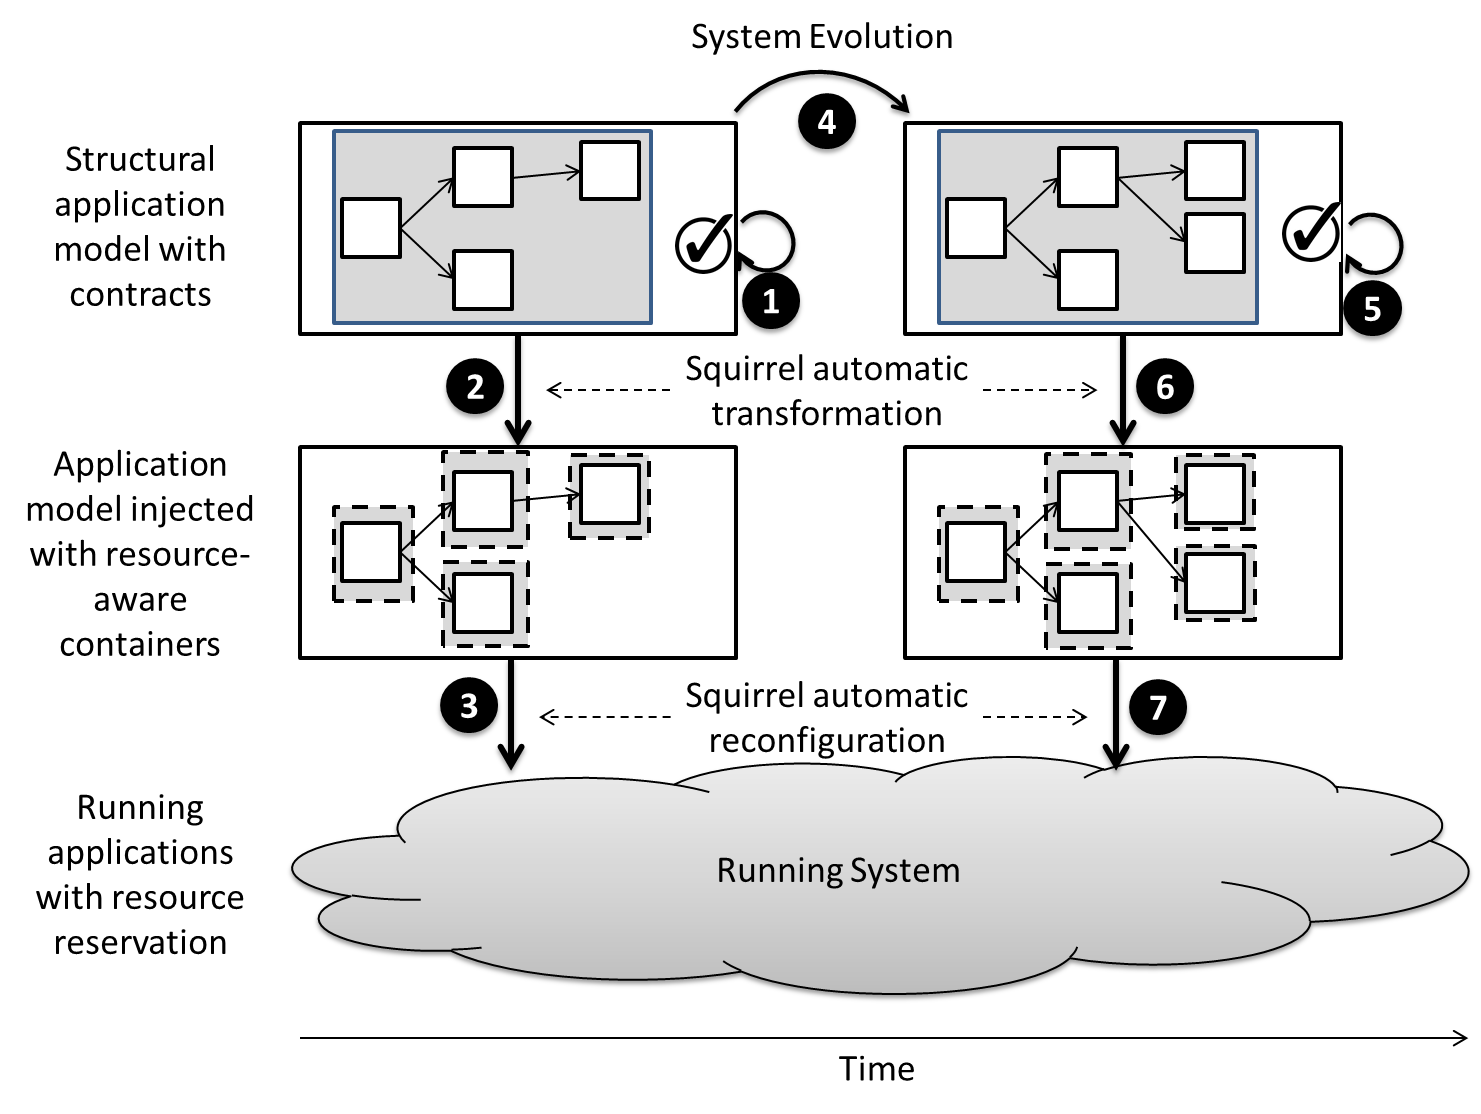
\includegraphics[width=0.7\textwidth]{chapter4/figures/globalOverview.png}
\caption{Squirrel approach for resources reservation} \label{fig:Overview}
\vspace{-0.5cm}
\end{figure}	

As illustrated in figure~\ref{fig:Overview}, Squirrel follows an automatic process to manage resources.
Squirrel receives an application's model, enhanced with contracts on resource reservation. 
Squirrel performs admission control to check the validity of the contracts on resource usage with respect to the available resources in the execution environment.
If the contracts are consistent with available resources, the process continues, if not, the application's model is refused.
Then, as depicted by arrow 2, Squirrel automatically transforms components or the configuration/architecture model by isolating components in resource-aware containers that can be finely configured to decrease the resource management overhead.
Finally, as depicted by arrow 3, Squirrel reconfigures the running system.
When the application evolves (arrow 4), 
%Squirrel automatically adapts the system while preserving resource reservation properties by applying the whole process on the new model (arrow 5, 6 and 7).
Squirrel attempts to preserve resource reservation properties while processing the new model (arrow 5, 6 and 7).


\subsection{Describing resource management requirements}
Beugnard et al. discuss the extending Meyer's \textit{Design-By-Contract} idea to software components~\cite{Beugnard774917}.
They classify component contracts into four categories: syntactic (level 1), semantic (level 2), synchronization (level 3), and Quality of Service (level 4).
%They explain that component contracts have to deal with concerns that they classified into 
%Fifteen years later, many component-based frameworks provide contracts that are used to: 
%i) Describe the component features with all required contracts.
%ii) Select from all contracts those that are useful in the context of component use, and configure them.
%iii) Evaluate contracts and react accordingly.
%iv) Decide when to stop evaluating contracts. 
There is no de-facto standard to describe component contracts, but many domain specific interface description languages contain such metadata.
This chapter assumes that components have contracts to deal with resource reservation (level 4).
A contract in Squirrel defines component resource requirements written in terms of resource types, quotas and expected component usage.
\begin{itemize}
\item{\textbf{Definition 1}} A resource type indicates any class of computational resource that is useful to a component.
Its consumption must be susceptible to monitoring and reservation.
In this paper, we consider CPU, Memory, Network Bandwidth and IO Throughput.

\item{\textbf{Definition 2}} Expected component usage describes the expected number of external invocations of each method of the component interface.
In short, let $C$ be a component instance, then $\forall{I \in C_{Interfaces}}, \forall{M \in I_{methods}} \\ {EU}_{IM}$ is the number of expected invocations of method $M$, per second.

\end{itemize}

A \textbf{contract in Squirrel} is a set of tuples with the form $\langle RT, N, MU \rangle$ where $RT$ is a resource type, N the maximum amount of resources to reserve, and $MU$ is the measuring unit used for this resource type.
Optionally, Squirrel supports the definition of a set of tuples with the form $\langle I, M, {EU}_{IM} \rangle$ where $I$ is a component interface, $M$ is a method of the interface, and ${EU}_{IM}$ the expected usage.
Implementations of the Squirrel approach must provide a way to define contracts with these concepts.
%In section~\ref{sec:kevoree} 
We use a domain-specific language to describe contracts.

\subsection{Admission control} \label{sect:admissionControl}

Providing resource reservation in a component based framework requires checking if components' resource-aware contracts are compatible with the resources available in the execution environment.
%The platform provides a fixed amount of resources that constitute the pool of resources used by components.
By checking the availability of resources, the platform controls component admissions.

%To support this dynamism while managing resources, 
To support resource management at runtime, Squirrel takes into account two events: i) component deployment, and ii) component removal.
%These are common operations on any middleware; hence adding a notification for these events is straightforward.
Whenever the application is modified, the system automatically recalculates the aggregated resources required by the application and compares it to the available resources in the execution environment.
If the available resources are greater than those required by the application, the reconfiguration is accepted, else, the application model is refused and the reconfigurations are discarded.

%\subsection{Defining multiple variants of execution model}
%\todo{I couldn't finish this, so I'm writing my ideas}
%To support our approach, a middleware needs to support multiple ways of mapping component instances into system/runtime abstractions.
%Somehow, it means that it needs an extension point to describe a factory for creating component instances.
%I can see two ways of doing so, either the writer of the middleware provides many versions of execution model or she provides a mechanism to extends the semantic of a component instance and of component containers (Node).
%In Kevoree we achieved this easily because it is naturally extensible, we can define new Node Types, New Channel Type, and we can compose them.
%Moreover, we use Models@Runtime to easily change between variant of mappings (e.g., we receive a model where each component is executed as a Thread and sometime we transform the model in order to execute components as processes). 

\subsection{Mapping component-model concepts to system-level abstractions}

%To map component-model concepts to system-level abstractions that allow for resource management, Squirrel defines steps to perform either during the design/implementation of the platform or at deployment time.
Squirrel defines steps to map component-model concepts to system-level abstractions that allow for resource management. Mappings can be applied during the design and implementation of the framework, or at deployment-time.
During framework design/implementation, developers identify system abstractions that are suitable to represent each concept and implement the respective mappings.
As a second step, resource management methods for each abstraction are implemented and evaluated.
This evaluation is used to determine the management methods with lowest overhead for each pair of system abstraction and resource type.
Later on, at deployment-time, the platform selects a component-to-system mapping using optimization techniques and the data obtained at design-time.
In this section, we briefly explain each step.

As we have mentioned, components can be represented through different system abstractions. % in the runtime platform.
This requires \textit{identifying possible mappings from components to system-level abstractions}.
Mappings must respect the semantics of the component model, and %but for a resource-aware platform, 
must provide resource management capabilities.
A key problem is that different mappings have different non-functional properties, and optimizations are often needed to make the mappings attractive. % competitive.
Additionally, an extensible design of the component platform, where it is easy to accommodate new mappings, greatly facilitates the co-existence of different mappings to represent a component. 
The set $ \textit{SA} $ of system abstractions that are available to represent a concept, along with the recommended optimizations for each abstraction, are defined in this step.

During the design/implementation of the platform it is necessary to \textit{define methods to manage resources} for each pair of system abstraction and resource type.
Developers must devise resource management methods for each mapping
% and resource type, 
 and identify the least costly.
If we consider different abstractions and resource types, we can define the matrices $ M $ and $ C $ where
$ \forall{\textit{sa} \in \textit{SA}, \textit{rt} \in \textit{RT}} $ the values
$  M_{\textit{sa}, \textit{rt}} $ and $ C_{\textit{sa}, \textit{rt}} $ indicate the method that minimizes the cost of managing the resource $ \textit{rt} $ when the abstraction $ \textit{sa} $ is used to represent a component. %, and this minimum cost.
%\hl{In a simple setting, the cost of each pair could be calculated as the mean overhead produced by the management method when some benchmarks are executed.[IS THIS PHRASE NECESSARY?]}
We make two assumptions about the resource management mechanisms: i) mechanisms are always composable if they manage different resource types, and ii) the costs of any pair of management mechanisms are independent.

At deployment-time, \textit{the platform selects the mapping} to use for each component in the application. % to deploy.
To do so, the platform uses the information contained in the matrices $ M $ and $ C $, the set of possible optimizations for each mapping, and the resource requirements of the application.
At this stage, the only data needed regarding resource requirements is the type of resource.
%Using this data, it is possible to apply an optimization method to select the best mapping candidate.
Using this data allows selecting the best mapping candidate.
Although we only use a single cost matrix that contains the overhead of each management mechanism, we think it is easy to generalize the approach to handle multi-objective optimizations with more than one cost matrix.
Others refinement to evaluate the cost of a mapping are possible.
For instance, we can consider the cost of using a specific binding to connect two components that use a given mapping.
Finally, there are many optimization methods that can compute the mappings, we do not propose any particular method in the approach.
However, the results shown in section~\ref{sec:evaluation} suggest that very simple heuristics can lead to good performance. 
 

%\todo{Here we should talk about the heuristic. We are trying to optimize, so we need to choose a mapping for each component. We only have a partial information about each resource managment mechanism. that's why we cannot perform classic optimization and we relies on heuristics}
%\todo{A conclusion here}


\section{Reference Implementation} \label{sec:kevoree}
%\fixme{The beginning of this section needs work, it starts by saying we introduce kevoree, then introduces models@run.time, then kevoree.}

Squirrel's reference implementation exploits the modesl@run.time approach and provides resource-awareness capabilities to the Kevoree component framework~\cite{Fouquet:2012:DCM:2304736.2304759}.
%to support models@run.time.
%We begin with a brief overview of Kevoree.
%Built on top of dynamic component frameworks, models@run.time denotes model-driven approaches to tame the complexity of dynamic adaptation~\cite{Morin:2009:TDA:1555001.1555028}.
Models@run.time denotes model-driven approaches to tame the complexity of dynamic adaptation~\cite{Morin:2009:TDA:1555001.1555028}.
%It pushes the idea of reflection one step further by considering the reflection-layer as a model.
The ``model at runtime'' is a reflection model that can be decoupled from the application (for reasoning, validation, and simulation purposes) and then automatically resynchronized.
Models can manage not only the application's structural information (i.e., the architecture), but can also be populated with other information, such as runtime monitoring data.

Kevoree is a component framework for distributed systems that builds and maintains a structural model of the system, following the models@run.time paradigm.
%and builds a structural model of the distributed system.
Kevoree is mainly used because: (i) it presents a snapshot of the distributed system, and (ii) it provides a language to drive the reconfigurations. 
\textit{Component} and \textit{Channel} are two of the concepts used in Kevoree models.
The former represents software units that provide the business value.
The latter, with the same role as connectors, are in charge of inter-component communication.
Channels encapsulate communication semantics (e.g., synchronous, unicast).

\subsection{A resource-aware container for CPU and I/O reservation} \label{sec:cgroups-based-reservation}

Our implementation leverages resource-reservation mechanisms at the system-level to provide containers for CPU and I/O reservation.
More specifically, it maps the concept of \textit{container} onto a \textit{cgroup}.
Both \textit{containers} and \textit{Kevoree components} are hierarchical structures that are easy to map onto cgroups' hierarchy.
Indeed, a container deploys components and a component runs threads.
To configure the container we setup a hierarchy of cgroups
using the following rules:
\begin{enumerate}
\item
%A fixed amount of resources are reserved for the Kevoree framework, which includes the components of the managed system. This serves as the upper resource-limit.
%To implement this rule we execute the Kevoree framework under a cgroup, while unmanaged applications are expected to run under other cgroups for isolation.
The Kevoree framework is started under a cgroup, using a fixed amount of resources that will be divided among the system's components. 
% that determines the total resource pool. % are reserved (for both).
%This value serves as the pool of resources the framework may use to deploy components.
%On the one hand, it is the maximum amount of resource the container will use when all the threads inside are demanding.
%On the other hand, it is the minimum amount it will receive when other applications outside the container are demanding.


\item
%We create a new resource-aware container for each component, represented by a cgroup.
Each component gets a new resource-aware container, also represented by a cgroup.
The component's contract is translated into a slice $S_c$ of the initial resource allotment, and the result is passed to
%configuration parameters to the cgroup.
the cgroup as configuration parameters.
A slice represents the
%minimum and maximum quantity of 
resources the component has available.
%This means that, although we support resource reservation, we are not supporting overcommitment.
%Since the scheduling unit for cgroups is a thread, we assign threads to cgroups in order to enforce resource reservation.
%However, we cannot assign threads directly to their component's cgroup because then all of them will obtain the same slice $S_c$.
%What we want is to share $S_c$ among all the threads within a component.
%Therefore, a \textit{hidden cgroup} is created that inherits the slice $S_c$ and provides a share to any thread assigned to it by using  \textit{Relative Shares Tunable Parameters}.

\item Since the scheduling unit for cgroups is a thread, we assign the component's threads to the cgroup to enforce resource reservation.

%\item Threads are assigned to the \textit{cgroup} created for the thread owner's component.
\end{enumerate}


\begin{figure}
\centering
%\usetikzlibrary{shadows,arrows}

% Define block styles  
\tikzstyle{cgroup_sty}=[draw, fill=white!20, text width=5em, text centered,
  minimum height=1.4em, rounded corners]

\tikzstyle{thread_sty}=[draw, thin, fill=yellow!20, text width=3em, text centered,
  minimum height=1.4em,dashed]

\tikzstyle{cgroup_container_sty}=[cgroup_sty,fill=gray!20]

\tikzstyle{cgroup_container_hidden_sty}=[cgroup_container_sty,dotted]


\tikzstyle{line} = [draw, thick, color=black!80, -latex']

% commands
\newcommand{\cgroup}[2]{node (p#1) [cgroup_sty]
  {{\scriptsize{#2}}}}

\newcommand{\cgroupContainer}[2]{node (p#1) [cgroup_container_sty]
  {{\scriptsize{#2}}}}

\newcommand{\hiddenCgroup}[2]{node (p#1) [cgroup_container_hidden_sty]
  {{\scriptsize{#2}}}}

\newcommand{\thread}[2]{node (t#1) [thread_sty]
  {{\scriptsize{#2}}}}

\begin{tikzpicture}[scale=0.7,transform shape]
\path \cgroup {1} {Root CGroup};
\path(p1.south) + (-2,-1.2) \cgroupContainer {2} {Cgroup for Kevoree};
\path(p1.south) + (1.7,-1.2) \cgroup {3} {Cgroup for other apps};

\path(p2.south) + (2.3,-1.2) \cgroupContainer {4} {Cgroup for Component2};
\path(p2.south) + (-1.5,-1.6) \cgroupContainer {5} {Cgroup for Component1};

%\path(p4.south) + (0,-1.0) \hiddenCgroup {6} {Hidden Cgroup};
%\path(p5.south) + (0,-1.0) \hiddenCgroup {7} {Hidden Cgroup};

\path [line] (p1) --  node [left] {50\%} (p2);
\path [line] (p1) --  node [right] {50\%} (p3);

\path [line] (p2) --  node [left] {45\%} (p4);
\path [line] (p2) --  node [left] {10\%} (p5);
%\path [line] (p5) --  node [left] {100\%} (p7);
%\path [line] (p4) --  node [right] {100\%} (p6);

\path(p5.south) + (-1.5,-1.2) \thread {1} {Thread1};
\path(p5.south) + (1.8,-1.0) \thread {2} {Thread3};
\path(p5.south) + (0,-1.7) \thread {3} {Thread2};

\path(p4.south) + (0,-1.2) \thread {4} {Thread4};

\path [line] (p5) --  node [above,left] {33\%} (t1);
\path [line] (p5) --  node [above,right] {33\%} (t2);
\path [line] (p5) --  node [left] {33\%} (t3);

\path [line] (p4) --  node [right] {100\%} (t4);

\end{tikzpicture}
\caption{Reserving CPU by mapping components to cgroups} \label{fig:Mapping}
\vspace{-0.5cm}
\end{figure}

This scheme is used for CPU, I/O throughput and network bandwidth.
Each type of resource requires a different \textit{container type}.
% since configuring the container depends on varying properties defined on each cgroup subsystem.
Figure \ref{fig:Mapping} shows an example 
%of how our implementation uses 
using cgroups to reserve CPU for a system with two components.
In the tree, every edge is labeled with the cgroup's CPU slice.
% the cgroup obtains from its parent.
A slice is set for Kevoree, while unmanaged apps are maintained in separate containers.
Applying rule 2, CPU slices are assigned to \textit{Component 1} and \textit{Component 2} according to their resource contracts.
Following rule 3, every thread in \textit{Component1} receives $ 33\% $ of the component's slice.
%When configuring the containers, we apply rule 2 and assign \textit{Component 1} and \textit{Component 2} CPU slices according to their resource contracts.
%Finally, slices for Kevoree and for the rest of the system are assigned.
%In our case, we selected as description the number of instructions the container is able to execute because, as we show in section \ref{contracts}, our contracts use number of instructions in their definition. 
%For instance, if we assume that our container is able to execute 1002000012 instructions per seconds and we use the contracts in listing \ref{} then we obtain slices as in Figure \ref{Mapping}.
%\todo{Inti: create contracts for 2 components, 102345600 and 456789010 instructions}
%Finally, slices for Kevoree and for the rest of the system are assigned.
%This requires taking into account the trade-off between resource for components in Kevoree and for applications outside Kevoree.

%Assigning little resources to Kevoree allows external applications to execute smoothly but the number of admitted components in Kevoree decreases.
%On the contrary, if Kevoree uses a big slice then the performance of other applications is affected.

\subsection{Containers for Memory reservation} \label{overview-memory-reservation}

Memory reservation poses a unique challenge.
% for the usage of cgroups from within the Java runtime.
Although there is a cgroup-hierarchy for memory, it is not well suited for shared memory because the subsystem cannot precisely account for the consumption of each thread.
As a result, if we use cgroups to deal with memory, accounting would depend on the behavior of the garbage collector, which is hard to predict.
That makes cgroups inadequate to check or enforce component contracts in a single JVM process.
We have devised two mechanisms
%to represent containers for memory reservation.
to serve as memory containers.
In the first mechanism, all containers exist in a single process and resource limits are enforced by leveraging previous approaches
%to resource monitoring for Java (e.g., using bytecode instrumentation to account for consumption).
that use bytecode instrumentation to account for consumption.
The second mechanism
%delegates reservation to a lower level in the software stack by isolating
isolates components into new processes and then uses cgroups. % for resource management.
The rest of the section describes both solutions.

\subsubsection{Memory management based on monitoring.}
A memory reservation container ensures that its components have access to the memory they require.
Memory requests should only fail if a component violates its contract.
Implementing such a container is simple if memory monitoring is available at the application-level and memory requests are intercepted.
%DO WE NEED THIS PART?
%A container is a service that receives notifications when a component is violating its contract and then takes action to forbid future memory requests until a proper utilization level is reached.   
We use Scapegoat \cite{gonzalezherrera:hal-00983045} for memory consumption monitoring by defining multiple memory-aware containers within a single JVM.
In short, each container registers its component in ScapeGoat and receives a notification if a component violates its contract.
%This has an impact on the application's performance 
This introduces CPU and memory overhead for each component because of the instrumentation code.
%the instrumentation code imposes penalties on CPU/memory during the execution time of each component.
The main advantages are portability and simplicity.

\subsubsection{Isolation of components in separate processes.}
The second approach maps each container onto a separate process.
Reservation is achieved using cgroups as described in section \ref{sec:cgroups-based-reservation}.\footnote{In practice, we use cgroups to reserve memory, but we also bound the Java Heap to limit the consumption in Java code.}
%
%Reducing deployment time and complexity is critical since we deal with continuous deployment; hence we aim at automating the process of component isolation.
To do so, we start from an extended deployment model as shown in figure \ref{fig:Overview}.
%A transformation follows the rules below is applied to the model:
The model is then transformed using the following rules:
\begin{enumerate}
\item  Component isolation: each \textit{set of components} with a shared memory contract is isolated in a separate \textit{JVM node} within the same \textit{physical device}.
%A contract regarding memory reservation is shared if the involved components reside in the same \textit{JVM node} in the source model.
\label{rule1-model-transformation} 

%\item Channel adjustment: Every channel that connects two components in the source model that is isolated in the target model (by the application of rule \ref{rule1-model-transformation}) is adjusted to reflect the semantics of the source model. This includes changing the channel type as well as modifying some of its properties.
\item Channel adjustment: channels that connect isolated components are updated to reflect the semantics of the source model. This includes changing the channel type and modifying some of its properties.
\end{enumerate}
The resulting model can be deployed.
%in the newly created Kevoree instances through a dedicated \textit{Kevoree Group}.

%Figure~\ref{model_transformation} shows how to transform the model of a simple application.
%In this case, we assume that every component has its own contract regarding memory reservation.
%Following the rules, we only need to create an additional \textit{JVM node} and to adjust the \textit{channel} that connects components \textit{Video Recorder} and \textit{Video Coder}.  

%\begin{figure*}
%\centering
%\usetikzlibrary{shadows,arrows}
\pgfdeclarelayer{background}
\pgfdeclarelayer{foreground}
\pgfsetlayers{background,main,foreground}

% Define block styles  
\tikzstyle{component_sty}=[draw, fill=white!20, text width=5em, text centered,
  minimum height=1.4em, rounded corners]

\tikzstyle{deployment_node_sty}=[draw, thin, text width=2.5em, text centered,
  minimum height=1.4em]

\tikzstyle{physical_node_sty}=[deployment_node_sty, fill=yellow!20, text width=2.5em, dashed]

\tikzstyle{virtual_node_sty}=[deployment_node_sty, fill=gray!30, dotted]

\tikzstyle{line} = [draw, thick, color=black!80, -latex']

\tikzstyle{channel_sty}=[draw, fill=green!20, text width=5em, text centered,
  minimum height=1.4em, dashed]


% commands
\newcommand{\component}[2]{node (p#1) [component_sty]
  {{\scriptsize{#2}}}}

\newcommand{\virtualNode}[2]{node (p#1) [virtual_node_sty]
  {{\scriptsize{#2}}}}



\begin{tikzpicture}[scale=0.9,transform shape]

\begin{pgfonlayer}{foreground}
	\path \component{1} {Video Recorder};
	\path (p1.south) + (0,1) \component{2} {Video coder};
	\path (p1.east) + (2.2,0.0) \component{3} {Video storage};
\end{pgfonlayer}

%\path \virtualNode{1} {node0};

% virtual node 0
\path (p2.west)+(-0.16,0.6) node (g) {};
\path (p1.east)+(0.16,-0.8) node (h) {};
\path[virtual_node_sty] (g) rectangle (h) ;
%\path (h) +(-1.3,0.2) node (asrs) {java node 0};
\begin{pgfonlayer}{background}
% physical node 0
        \path (g.west)+(-0.12,0.24) node (g) {};
        \path (h.east)+(0.12,-0.24) node (h) {};
        \path[physical_node_sty] (g) rectangle (h);
     	\path (h) +(-1.6,-0.2) node (asrs) {device 0};         
\end{pgfonlayer}

% virtual node 1
\path (p3.west)+(-0.16,0.6) node (g) {};
\path (p3.east)+(0.16,-0.8) node (h) {};
\path[virtual_node_sty] (g) rectangle (h) ;
\path (h) +(-1.3,0.2) node (asrs) {java node 1};
\begin{pgfonlayer}{background}
% physical node 1
        \path (g.west)+(-0.12,0.24) node (g) {};
        \path (h.east)+(0.12,-0.24) node (h) {};
        \path[physical_node_sty] (g) rectangle (h);
     	\path (h) +(-1.6,-0.2) node (asrs) {device 1};         
\end{pgfonlayer}

%channels
\path (p2) + (-2.5,-0.2) node (channel1) {};
\path [line] (p1.west) -- (channel1) ;
\path [line] (channel1) --  (p2.west);
\path[channel_sty] (channel1) circle (0.4);

\path (p1) + (2.3,2.1) node (channel2) {};
\path [line] (p2.north) -- (channel2) -- (p3.north);
\path[channel_sty] (channel2) circle (0.4);

\path (h) node (temp1) {};

%AFTER MODEL TRANSFORMATION

\path (temp1.east) + (0.1,4) node(l0) {}; 
\path (temp1.east) + (0.1,-1) node(l1) {};
\path[draw, thick, color=black!80, dashed] (l0) -- (l1);

\begin{pgfonlayer}{foreground}
	\path (temp1.east) + (2,1) \component{1} {Video Recorder};
	\path (p1.east) + (1.6,0) \component{2} {Video coder};
	\path (p2.east) + (2.2,0) \component{3} {Video storage};
\end{pgfonlayer}

% virtual node 0
\path (p1.west)+(-0.16,0.6) node (g) {};
\path (p1.east)+(0.16,-0.8) node (h) {};
\path[virtual_node_sty] (g) rectangle (h) ;
\path (h) +(-1.3,0.2) node (asrs) {java node 0};
% virtual node 1
\path (g) node (gTemp) {};
\path (p2.west)+(-0.16,0.6) node (g) {};
\path (p2.east)+(0.16,-0.8) node (h) {};
\path[virtual_node_sty] (g) rectangle (h) ;
\path (h) +(-1.3,0.2) node (asrs) {java node 1};
\begin{pgfonlayer}{background}
% physical node 0
        \path (gTemp.west)+(-0.12,0.24) node (g) {};
        \path (h.east)+(0.12,-0.24) node (h) {};
        \path[physical_node_sty] (g) rectangle (h);
     	\path (h) +(-3,-0.2) node (asrs) {device 0};         
\end{pgfonlayer}

% virtual node 1
\path (p3.west)+(-0.16,0.6) node (g) {};
\path (p3.east)+(0.16,-0.8) node (h) {};
\path[virtual_node_sty] (g) rectangle (h) ;
\path (h) +(-1.3,0.2) node (asrs) {java node 2};
\begin{pgfonlayer}{background}
% physical node 1
        \path (g.west)+(-0.12,0.24) node (g) {};
        \path (h.east)+(0.12,-0.24) node (h) {};
        \path[physical_node_sty] (g) rectangle (h);
     	\path (h) +(-1.6,-0.2) node (asrs) {device 1};         
\end{pgfonlayer}

%channels
\path (p2) + (-1.6,2.1) node (channel1) {};
\path (p2.north)+(-0.7,-0.2) node (tt0) {};
\path [line] (p1.north) -- (channel1) -- (tt0);
\path[channel_sty] (channel1) circle (0.4);

\path (p3) + (-1.6,2.1) node (channel2) {};
\path [line] (p2.north) + (0.7,0) -- (channel2) -- (p3.north);
\path[channel_sty] (channel2) circle (0.4);


\path (h) node (temp1) {};

% legend
% physical nodes
\path (temp1)+(1.0,2.8) node (h) {};
\path (h)+(0.8,0.8) node (g) {};
\path[physical_node_sty] (g) rectangle (h);
\path[right,text width=4em] (g) +(0,-0.4) node (asrs) {physical devices};

% virtual nodes
\path (h)+(0,-0.9) node (h) {};
\path (g)+(0,-0.9) node (g) {};
\path[virtual_node_sty] (g) rectangle (h);
\path[right] (g) + (0.0,-0.4) node (asrs) {virtual nodes};

% components
\path (h)+(0,-0.9) node (h) {};
\path (g)+(0,-0.9) node (g) {};
\path[component_sty] (g) rectangle (h);
\path[right] (g) +(0,-0.4) node (asrs) {components};

% channels
\path (g)+(-0.4,-1.35) node (g) {};
\path[channel_sty] (g) circle (0.4);
\path[right] (g) +(0.38,-0.0) node (asrs) {channels};

\end{tikzpicture}
%\caption{Transforming deployment model to achieve memory reservation} \label{model_transformation}
%\end{figure*}

\paragraph{Runtime initialization through cloning.}
The approach to memory reservation based on isolation deploys each \textit{set of components} into separate processes.
This involves two steps: creating new instances of the runtime, and deploying a \textit{set of components} on each instance.
To reduce deployment time, instead of starting processes from scratch,
%we create clones of a base runtime for new instances.
new instances are cloned from a base runtime.
The base runtime is created offline. %, is used to deploy components through fast cloning and configuration.
Both steps, base runtime creation and cloning, are based on CRIU.\footnote{\url{criu.org}}
This tool allows snapshoting a process and starting any number of clones from the snapshot.
In essence this \textit{forks} the process.
%creating in practice a sort of \textit{forking} that is hard to perform otherwise.
%Afterwards, the cloned runtime is adapted by deploying a new model that includes an application's component.

%The implementation includes two classes of Kevoree instances, the management instance class $R_M$ and the base-instance class $R_b$.
%The former is a frond-end that interacts with external users and is in charge of: 1) modifying the model to support isolated deployment as section \ref{overview-memory-reservation} describes, 2) creating clones based on $R_b$ and, 3) sending messages to clones with the aim of deploying components.
%The $R_b$ class of instance executes a component that implements the system's adaptation by waiting for a message that includes the new model to deploy.

\paragraph{Channel for intra-node communication.}
Channels are meant to send arbitrary POJO structures from one component to another.
When components are isolated into separate processes,
%a channel transforms a POJO structure twice:
a channel must marshal and unmarshal the POJO using a representation suitable for inter-process communication.
%i) marshal the POJO into a representation suitable for IPC in the source and, ii) unmarshaling it in the destination.
In practice, a channel must copy data at least twice, no matter what IPC mechanism is used.
%This fact has an impact on the class of IPC mechanism we can leverage.

In this paper we propose a new channel for intra-node communication.
Communication is performed through a message queue built on top of shared memory using an alternative high-performance framework to serialize objects.
Each channel is mapped to a shared-memory region that hosts a synchronized queue of messages.
This region contains three sections: an array of blocks to store message chunks, 
a set of free blocks, and a circular queue in which an element points to a list of chunks.
We use the procedure described in \cite{Unrau:708530} to synchronize senders and receivers, but we also support broadcast semantics without unnecessary additional copies.
Our approach copies the POJO from the sender's heap to shared-memory during data marshaling, then every receiver makes a copy from shared-memory.
The implementation uses a high-performance serialization framework\footnote{\url{https://github.com/RuedigerMoeller/fast-serialization}}
% ~\cite{Moeller:2014:Online} 
instead of Java's built-in serialization mechanism
and is able to serialize arbitrary objects with better performance.
%by using alternative binary representation and its own cached reflection mechanism.


\section{Evaluation} \label{sec:evaluation}

%The Squirrel guidelines can be applied to component-based models for different platforms, but in this section we focus on evaluating our implementation for Kevoree.

This section presents experiments that determine the performance of our reference implementation.
We evaluate performance and overhead using systematic, full isolation of components using resource containers.
We also compare different design decisions presented in the previous section.
%We also compare the performance of the various design choices presented in the previous subsection against each other.
%We therefore perform the three following experiments:
The experiments include:
\begin{itemize}
 \item Measuring the CPU and memory overhead introduced by \textit{Scapegoat} and \textit{component isolation}.
 \item Determining how isolation affects deployment time and to what extent process cloning and our high-performance IPC alleviate it.
 \item Evaluating the extent to which known high-performance IPC techniques reduce communication overhead due to component isolation.
\end{itemize}


%To obtain comparable and reproducible results, 
We used the same hardware across all experiments: a laptop with a 2.90GHz Intel(R) i7-3520M processor, running Linux with a 64 bit kernel 3.13.5 and 8GiB of RAM.
We used the HotSpot JVM v1.7.0-55, and Kevoree framework v5.0.1.

\subsection{Evaluating performance overhead}
In section \ref{overview-memory-reservation}, we describe two approaches for memory reservation: 1) Scapegoat \cite{gonzalezherrera:hal-00983045}, an instrumentation-based resource management container, and 2) using isolated processes with cgroups. %with memory constraints as containers.  
%Throughout this paper, we have highlighted the advantages and drawbacks of both approaches regarding deployment time and inter-component communication degradation, but so far, we barely considered CPU and memory consumption.
%In this section we compare the overhead produced by these two approaches in terms of CPU and memory consumption.
%Since we tackle resource management in component-based systems, it is necessary to conduct the experiments with more than one component.
To compare the overhead produced by these approaches, we devised use cases that contain two components that execute a test from the Dacapo Benchmark Suite~\cite{Blackburn:2006:DBJ:1167473.1167488}.
These components run in parallel to simulate realistic conditions where components demand resources simultaneously.
The use cases are executed with different settings, as follows:
\begin{enumerate}
\item Using cgroups to assign 50\% of the CPU time to each component (no memory monitoring).
Both components run on a single Kevoree instance with 2GiB maximum heap size.
This is the baseline because there is no CPU nor memory overhead.
Nevertheless, execution time is affected due to the CPU allotment.
We call this setting \textit{Memory unaware}.

\item Using \textit{Scapegoat} to monitor per-component memory consumption and bounding CPU consumption to 50\%.
Again, both components run on the same Kevoree instance with 2GiB maximum heap size.

\item Isolating each component in a new process, allotting 256MiB of memory to each process, and bounding its CPU consumption to 50\%.
\end{enumerate}

%\lstset{frame=tb,
  aboveskip=3mm,
  belowskip=3mm,
  showstringspaces=false,
  columns=flexible,
  basicstyle=\color{black}\scriptsize,
  numbers=none,
  numberstyle=\color{gray}\scriptsize,
  keywordstyle=\color{blue}\scriptsize,
  commentstyle=\color{dkgreen}\scriptsize,
  stringstyle=\color{purple}\scriptsize,
  breaklines=true,
  breakatwhitespace=true,
  tabsize=2,
  captionpos=b,
  language=java
}

%\begin{lstlisting}[escapeinside={(*}{*)},
%caption=Dacapo-Component-Type executes a benchmark,
%label=lst:component-with-benchmark,
%float=!h]
%run (String benchmarkTestName)
%	sleep(5) // wait for the other components
%	// if channel's latency is low, this is a sort of barrier
%	if master
%		channel.send(time)
%		time <- channel.receive
%	else
%		time <- channel.receive
%		channel.send(time)
%	// after the barrier, both components are synchronized
%	elapsedTime = dacapo.execute(benchmarkTestName)
%\end{lstlisting}

To measure CPU overhead, we use the result reported by each \textit{Dacapo test} and we keep the maximum value.
Measuring memory overhead is more complex because the garbage collector hides the real consumption.
We address this by approximating the consumption with the usage after each major garbage collection.
As there are many collection cycles during the use case's execution, and because we may have more than one runtime involved, we define a scheme to aggregate the values: the consumption $MC_i$ of every Kevoree instance is the maximum among all the usages reported after each collection, while the final consumption is defined as $\sum_{i \in \mathit{Isolates}} {\textit{MC}}_i$.

Figure \ref{fig:cpu-overhead} depicts the CPU overhead for \textit{Scapegoat} and \textit{Isolating components}.
%As an instrumentation based solution,
The overhead of \textit{Scapegoat} was expected because of the instrumentation.
On average, it performs 2.27 times worse than \textit{Memory Unaware}, which is consistent with \cite{gonzalezherrera:hal-00983045}.
In contrast, isolating components produces no appreciable CPU overhead for these use cases (small differences are likely due to environment fluctuations) because the components do not interact.

%Memory consumption is affected by both \textit{ScapeGoat} and \textit{Squirrel}.
Both \textit{ScapeGoat} and \textit{Isolating components} cause memory overhead.
As shown in figure \ref{fig:memory-overhead}, \textit{ScapeGoat's} is higher than when using component isolation.
\textit{Isolating components}'s overhead is the result of JVM duplication and is, on average, 99\% over baseline.
Meanwhile, \textit{ScapeGoat's} overhead is due to tagging objects with the identifier of the component that owns it.
Tagging adds either a field and a finalization method to an object, or wraps the object with a \textit{weak reference} held by the framework, resulting in overhead in the \textit{Permanent Space}.
%The overhead of these additional structures plus the burden of finalization methods in the \textit{Permanent Space}.
As seen in the experiments, memory overhead due to tagging is more important than CPU. 

\begin{figure*}

\subfloat[][]{
	\centering
	\begin{minipage}{0.48\textwidth}
	
\pgfplotstableread{
{Test Case}    {Memory Unaware}   {Scapegoat}   {Squirrel} 
xalan	7.910	9.9616	7.957
avrora	10.3672	11.6296	10.3214
batik	1.5054	2.0536	1.3078
fop	0.4774	3.6102	0.4708
luindex	0.7798	1.007	0.6836
lusearch	0.863	6.068	0.935
%pmd	125444	135085	125085
}\data

\begin{tikzpicture}[scale=0.9,transform shape]
  
\begin{axis}[
	every axis legend/.append style={nodes={right}},
	height=4.2cm, width=1\columnwidth,
    ybar=0pt,   % Stacked horizontal bars
    ymin=0,         % Start x axis at 0
    xtick=data,     % Use as many tick labels as y coordinates
    xticklabels from table={\data}{Test Case},  % Get the labels from the Label column of the \datatable
    scaled y ticks = false,
   	y tick label style={
   		/pgf/number format/1000 sep = \thinspace % Optional if you want to replace comma as the 1000 separator 
   	},
    scaled x ticks = false,
   	x tick label style={
   		/pgf/number format/1000 sep = \thinspace % Optional if you want to replace comma as the 1000 separator 
   	},
   	x tick label style={rotate=45},
    bar width = 4,
    ylabel={Execution Time (sec)},
    y label style={at={(0.1,0.5)}},
    legend pos=north west,
    legend style={at={(0.44,0.95)}},
    legend style={font=\tiny},
]
\addplot [fill=white] table [y={Memory Unaware}, x expr=\coordindex] {\data};
\addplot [draw=black,fill=black] table [y={Scapegoat}, x expr=\coordindex] {\data};    % Plot the "First" column against the data index
\addplot [draw=black,pattern=crosshatch] table [y={Squirrel}, x expr=\coordindex] {\data};
\legend{Memory Unaware, Scapegoat, Isolating components}
\end{axis}
\end{tikzpicture}
	\end{minipage}
	\label{fig:cpu-overhead}
}%
\subfloat[][]{
	\centering
	\begin{minipage}{0.48\textwidth}
	
\pgfplotstableread{
{Test Case}    {Memory Unaware}   {Scapegoat}   {Squirrel} 
xalan	30082990.4	393385183.2	53634089.6
avrora	30980142.4	104351584	47699702.4
batik	151662422.4	324599222.4	172317585.6
fop	72838632	756471347.2	97060990.4
luindex	36728345.6	98952945.6	57629534.4
lusearch	23896294.6666667	1182045168	109559376
%pmd	125444	135085	125085
}\data

\begin{tikzpicture}[scale=0.9,transform shape]
  
\begin{axis}[
	every axis legend/.append style={nodes={right}},
	height=4.2cm, width=1\columnwidth,
    ybar=0pt,   % Stacked horizontal bars
    ymin=0,         % Start x axis at 0
    xtick=data,     % Use as many tick labels as y coordinates
    xticklabels from table={\data}{Test Case},  % Get the labels from the Label column of the \datatable
    ytick={268435456,536870912,805306368,1073741824},
    scaled y ticks = false,
   	scaled y ticks=manual:{}{\pgfmathparse{#1/(1024*1024)}},
   	x tick label style={rotate=45},
    bar width = 4,
    ylabel={Memory Usage (MiB)},
    y label style={at={(0.01,0.5)}},
    legend pos=north west,
    legend style={font=\tiny},
]
\addplot [fill=white] table [y={Memory Unaware}, x expr=\coordindex] {\data};
\addplot [draw=black,fill=black] table [y={Scapegoat}, x expr=\coordindex] {\data};    % Plot the "First" column against the data index
\addplot [draw=black,pattern=crosshatch] table [y={Squirrel}, x expr=\coordindex] {\data};
%\legend{Memory Unaware, Scapegoat, Squirrel}
\end{axis}
\end{tikzpicture}
	\end{minipage}
	\label{fig:memory-overhead}
}%
%\hspace{4cm}
\caption{In \ref{fig:cpu-overhead}) and \ref{fig:memory-overhead}), we show CPU and memory overhead, respectively, caused by resource management during the execution of Dacapo benchmarks.}
\vspace{-0.5cm}
\end{figure*}


In synthesis, \textit{Isolating components} produces no CPU overhead, and low memory overhead in comparison to the performance of the same component model without resource management features.


\subsection{Evaluating starting time}
%In this subsection w
We compare the performance of three methods to deploy components: 1) in a single JVM (the baseline), 2) in isolated JVMs, starting processes from scratch, and 3) in isolated JVMs using CRIU to clone processes.
%a preexistent Kevoree runtime.
%In this experiment, 
We study the scalability of each method
% when many components are deployed.
 by deploying many components.
To do so, we created a template architectural model with two component types: \textit{Component A} runs in the \textit{management runtime} and deploys a new architectural model with resource-aware contracts; and \textit{Components B} records the timestamp after initialization is completed.
The experiment is as follows:
\begin{enumerate}
\item Component \textit{A} is deployed in the \textit{management runtime}. Afterwards, it forces the deployment of a new model with components of type \textit{B}.
\item After deployment, each component $c \in List_B$ sends \textit{A} the timestamp $T_c$.
\item Component \textit{A} collects $T_c - T_0, \forall {c \in List_B}$, where $T_0$ is the timestamp before deployment.
\end{enumerate}
 
\begin{figure}
\centering

\pgfplotstableread{
Components    {Processes} {CRIU}   {Plain Kevoree} 
%3        	  547.9745857	2529.407146	155.59293
%4     		  685.5744837	4341.203728	161.0288691
%5       	  743.4672428	5893.812401	171.0221846 
%7       	  1064.555133	9324.145486	162.0639121
%9       	  1268.435203	12563.95009	170.3004435
%12       	  1553.555575	17342.69007	172.6008458
%15 			  2045.492792	22165.56394	192.4309822
3	2.32911218644444	0.790383362555555	0.0907548736666666
4	3.68871036625	1.26219532775	0.12180777075
5	5.15906548553333	1.75811954106667	0.123942168
7	8.10203280628571	2.64415631295238	0.155080078
9	11.3615227505555	3.43788487492592	0.1576709236
12	16.3622474985	5.04937113155556	0.159263136583333
15	21.1857631248444	6.87974225997778	0.1994543878
}\Rapperswil

\begin{tikzpicture}[scale=0.8,transform shape]
  
\begin{axis}[
	every axis legend/.append style={nodes={right}},
	height=4.2cm, width=0.95\columnwidth,
    ybar=0pt,   % Stacked horizontal bars
    ymin=0,         % Start x axis at 0
    xtick=data,     % Use as many tick labels as y coordinates
    xticklabels from table={\Rapperswil}{Components},  % Get the labels from the Label column of the \datatable
    xlabel={Number of components},
    scaled y ticks = false,
%	y tick label style={
%		/pgf/number format/1000 sep = \thinspace % Optional if you want to replace comma as the 1000 separator 
%	},
    scaled x ticks = false,
           x tick label style={
           /pgf/number format/1000 sep = \thinspace % Optional if you want to replace comma as the 1000 separator 
           },
    bar width = 7,
    ylabel={Time (seconds)},
    y label style={at={(0.04, 0.5)}},
    legend pos=north west,
    legend style={font=\tiny},
]
\addplot [fill=white] table [y={Plain Kevoree}, x expr=\coordindex] {\Rapperswil};
\addplot [draw=black,fill=black] table [y=CRIU, x expr=\coordindex] {\Rapperswil};    % Plot the "First" column against the data index
\addplot [draw=black,pattern=crosshatch] table [y=Processes, x expr=\coordindex] {\Rapperswil};
\legend{Plain Kevoree, CRIU, Processes}
\end{axis}
\end{tikzpicture}
\caption{Average deployment time per component using different strategies}
\label{fig:starting-kevorees-final}
\vspace{-0.5cm}
\end{figure}

Figure \ref{fig:starting-kevorees-final} shows the results for a varying number of components.
As expected, using plain Kevoree is faster than deploying with other methods.
Leveraging isolation with CRIU's process cloning is, on average, 19.75 times worse than plain Kevoree, and this overhead grows with the number of components.
This is because CRIU-based deployment still spawns new threads in order to clone and create new instances. 
Nevertheless, using process cloning instead of starting processes from scratch reduces the isolation overhead by a factor of 41.79.

\subsection{Evaluating communication}
We present two experiments that highlight how we mitigate the impact of isolation on communication performance. % by using well-established technologies.
First, we use a micro-benchmark to compare the performance of a shared-memory based IPC queue and a socket-based IPC queue. % while sending blocks of data.
Then we benchmark the performance gain of using a specialized serialization framework that uses POJO structures, which is a common way to encode the business logic in real-life applications.
   
We evaluate our channel by comparing its performance against built-in TCP communication, which is a widely used IPC mechanism in Java.
To measure latency and bandwidth, the metrics we use for comparison, we developed a Netpipe clone~\cite{Snell96netpipe:a} for Java\footnote{Source code at: http://goo.gl/h7OVm5}.
The clone is delivered with three protocols: 1) socket-based, 2) our channel, and 3) a protocol for \textit{named pipes}.
The first uses simple TCP sockets with synchronous operation in its implementation. 
The second requires two channels, configured to use a queue with 128 chunks of 512Kb, because our channel is unidirectional.
Figure \ref{fig:latency-raw-communication} shows the latency for messages shorter than 128 bytes.
Memory-based communication outperforms NIO-sockets for all the values in the range.
Likewise, figure \ref{fig:badnwidth-raw-communication} shows the throughput of both mechanisms.
In general, memory-based communication behaves better than TCP sockets.
Our approach outperforms sockets by an average of 652.36\% for messages shorter than 512 bytes.
Meanwhile, it behaves on average 46.26\% better for messages between 1 Mb and 64 Mb, which is the range where the benefits of large copies surpass the disadvantages of having a synchronized queue.

\begin{figure*}
\centering
\subfloat[][]{
	\begin{minipage}{0.49\textwidth}
	
\pgfplotstableread{
{Data Size}    {NIO}   {Shared Memory}
0	6.298	1.58	
1	6.678	0.92	
1.5849625007	6.27	0.921	
2	6.914	1.012
2.5849625007	6.263	0.909
3	6.92	0.911
3.5849625007	7.14	0.918
3.7004397181	6.678	0.918
4	6.555	0.914
4.2479275134	6.536	0.917
4.3923174228	8.42	0.926
4.5849625007	6.243	0.924
4.7548875022	6.325	0.921
4.8579809951	6.324	0.921
5	6.243	0.915
5.1292830169	8.477	0.917
5.4918530963	7.925	0.925
5.5849625007	7.552	0.915
5.672425342	6.842	0.958
5.9307373376	8.49	0.997
6	8.484	1.199
6.0660891905	8.448	1.083
6.5391588111	8.467	0.946
6.5849625007	6.901	0.922
6.6293566201	8.48	1.104
6.9657842847	8.481	0.932
7	7.184	0.949
}\datatable

%\newcommand\test[1]{
%\pgfmathsetmacro{\var}{#1}
%\pgfmathparse{\varDelta*2} \pgfmathresult}

\definecolor{light-gray}{gray}{0.35}

\begin{tikzpicture}
    \begin{axis}[
    every axis legend/.append style={nodes={right}},
    width= 1\columnwidth,
    height=3.8cm,
    xlabel={Message Size (bytes)},
    ylabel={usec},
    %y label style={pos=east},
    y label style={at={(0.14, 0.5)}},
    x label style={at={(0.5, 0.08)}},
    legend pos=north west,
    legend style={anchor=north west,font=\tiny},
    xtick={0,2,4,6,7},
    %xmode=log,
    %log basis x={2},
    scaled y ticks = false,
    y tick label style={
    	/pgf/number format/1000 sep = \thinspace
    },
    x tick label style={font=\tiny},
    scaled x ticks=manual:{}{%
      	\pgfmathparse{pow(2,#1)}%
    },
    %xticklabel={\pgfmathprintnumber\tick },
    %scaled y ticks=manual:{}{%
    %      	\pgfmathparse{#1/1000}%
    %},
    yticklabel={\pgfmathprintnumber\tick},
    ]
    	\addplot [mark=+,color=black,mark size =1] table[y={Shared Memory}, x = {Data Size}] {\datatable};
    	%\addlegendentry{Shared Memory}[minimum height=1.9in];
    	\addplot [mark=none,color=gray] table[y={NIO}, x ={Data Size}] {\datatable};
    	%\addlegendentry{NIO}[minimum height=1.9in];
    \end{axis}
\end{tikzpicture}
	\end{minipage}
	\label{fig:latency-raw-communication}
}
\subfloat[][]{
	\begin{minipage}{0.49\textwidth}
	
\pgfplotstableread{
{Data Size}    {Shared Memory}   {NIO} {Named Pipe}
0	4.829262874	1.211303577	2.278292766
1	16.582080532	2.284973183	4.481888576
1.5849625007	24.84903843	3.650475913	7.285710353
2	30.169457071	4.413739735	8.817659304
2.5849625007	50.334063092	7.308872177	12.819947261
3	67.033301105	8.820402778	17.670900556
3.5849625007	99.710387763	12.822872274	25.811055873
3.7004397181	108.088504798	14.851562274	27.280316859
4	133.5675669	18.621127822	35.125028568
4.2479275134	158.098159941	22.179711705	41.054803786
4.3923174228	172.936356172	19.027447421	44.744471279
4.5849625007	198.258407658	29.328904007	51.219885409
4.7548875022	223.640214426	32.568470093	57.679047943
4.8579809951	240.130104691	34.986339417	63.408061398
5	266.9337384	39.106509783	68.524550827
5.1292830169	291.07690972	31.501307665	75.133209088
5.4918530963	371.306741859	43.323522934	95.74922823
5.5849625007	400.371365819	48.490743999	102.375468435
5.672425342	406.104746267	56.872079534	109.795933895
5.9307373376	466.792042028	54.818062952	131.176356948
6	407.150323017	57.550038602	166.253173322
6.0660891905	471.989770733	60.505008949	145.084452028
6.5391588111	749.881978428	83.800438008	219.863148031
6.5849625007	794.093319162	106.139907555	205.538721338
6.6293566201	684.256935216	89.067641012	214.048927819
6.9657842847	1023.734636763	112.453472776	300.145881529
7	1029.584105149	135.930753075	309.12421058
7.0334230015	1027.304169707	116.697242107	285.318100698
7.5622424242	1372.861669051	168.699330324	450.216803756
7.5849625007	1520.213189906	178.617329882	412.373322461
7.6073303137	1487.353476166	223.004631634	414.142278358
7.9829935747	1883.964538087	304.945579899	544.718262454
8	2029.21174905	303.157529871	552.163844844
8.0168082877	2078.834554099	231.545405236	600.765062111
8.5736471875	3004.966139295	424.80696054	984.164634937
8.5849625007	2987.83168967	342.123641214	978.416557876
8.5961897561	2981.563745694	395.555755955	981.559766323
8.9915218461	3955.435559352	611.575583119	1262.459850305
9	3937.062130055	553.18025024	1105.547862345
9.0084286221	3949.038994648	578.762145252	1108.009672612
9.5793159376	5751.338984494	925.793618042	1667.525200127
9.5849625007	5763.6263342	683.90157147	1630.194166837
9.5905870499	5782.042290551	893.794979677	1943.390221041
9.9957671509	7375.253260315	1103.914749616	2555.347488896
10	7420.6583416	1085.280140642	2583.62773537
10.0042204663	7399.879239443	1130.343164423	2545.719136133
10.5821419817	10407.615838242	1528.461298638	3836.099253253
10.5849625007	10459.010591026	1430.78942209	3885.122419844
10.5877775163	10467.367839251	1456.155914263	3378.080700848
10.9978851278	13413.996748093	1803.067395975	4378.763130842
11	13308.791104471	1746.102644706	4540.244522221
11.0021117765	13234.397107891	1994.433990999	5073.758245466
11.5835529305	14022.214827706	3058.174009469	9483.821893006
11.5849625007	17574.180581605	2551.424401063	8084.84927267
11.5863706951	17607.289599655	2533.045417625	8777.943762495
11.9989429514	16565.124813011	4983.721139081	14220.906836006
12	17038.373526088	3774.507385952	12201.364596254
12.0010562746	13210.648128855	4017.979668263	7307.280817184
12.5842578877	23084.476673518	4910.603339731	10086.517395917
12.5849625007	23871.089498227	4966.990490482	9730.990861993
12.5856667697	23709.790397143	5048.779860844	10043.171230086
12.9994715725	29257.910613264	9471.012935496	14228.934368891
13	28683.556655596	6233.173950593	14258.32114591
13.000528234	28549.362950889	7356.552861198	11784.156845751
13.5846102372	34413.107338882	8704.617585743	15821.282060252
13.5849625007	34421.08019242	8713.01377627	16389.392099268
13.5853146782	33561.250799983	10376.784988679	15029.013424612
13.9997358105	25595.465454619	10960.299110444	19477.406159846
14	20223.156583983	10978.068437467	18929.49199111
14.0002641412	25326.378293446	12459.412789012	18114.753416798
14.5847863797	26250.975590243	18111.530868468	23665.630920163
14.5849625007	26235.212219155	15523.929346838	24525.326782535
14.5851386002	25153.809591023	14975.096833361	22628.094517365
14.9998679113	31049.401914693	22139.146166433	26475.952243735
15	31287.197379148	20174.984879434	27180.220598481
15.0001320766	31270.213652828	22299.988561706	25833.004193619
15.5848744429	37764.33788921	24583.590207991	30892.539854137
15.5849625007	35904.006790762	24067.295665602	33595.235558465
15.5850505532	37394.07694005	21385.294903538	30253.574020233
15.9999339572	42024.611702048	22156.773973963	34400.577397926
16	42526.409381948	22768.653369153	33355.416041306
16.0000660398	42135.371754509	22095.615170307	24516.95346759
16.5849184725	46634.977226464	31544.055792361	27346.3375803
16.5849625007	46755.648430194	32020.413157657	27510.498278274
16.5850065276	46622.664838772	28171.132563909	27192.106104393
16.999966979	47238.234258162	29686.823448866	30109.450105664
17	47158.651696736	29563.339750158	29587.405439739
17.0000330203	47199.614834277	29597.736848209	25958.114070443
17.5849404868	45517.942281518	31879.906514408	29219.800949252
17.5849625007	41982.178237447	42632.564123951	29301.331769581
17.5849845143	42661.298716979	31764.349460218	26685.512778575
17.9999834896	46414.692794078	33266.028653703	29164.31928632
18	48395.722679253	33289.438190973	29288.477628167
18.0000165102	47313.280360889	33235.604391119	27216.297460076
18.5849514938	41963.793553975	34805.978837333	28980.488163916
18.5849625007	47278.064642522	34775.082842428	29063.752375911
18.5849735076	48572.455477075	34868.32660189	27847.458660613
18.9999917448	44726.216166649	35271.795693727	28712.569156876
19	43996.571385341	34852.366230723	30321.355537527
19.0000082551	44166.435569925	34783.859418754	27930.63156985
19.5849569973	47809.777463692	34134.247276319	28135.734709709
19.5849625007	50296.361907195	34030.893356802	27890.015515337
19.5849680042	48676.941303384	34022.599544173	27472.353309474
19.9999958724	38427.489532814	32070.098342443	26007.417473416
20	42256.795098438	32078.172520878	25816.481805726
20.0000041276	38698.881552732	38439.343773152	25608.293415362
20.584959749	35059.230140608	33797.506118382	23825.296573269
20.5849625007	35818.974880833	33265.916556813	23229.586947571
20.5849652524	34978.742656498	33338.510640811	23525.150646978
20.9999979362	34120.277968082	36638.090297614	22381.711044179
21	33559.886750483	30035.390170359	22159.744848227
21.0000020638	33559.501904135	36802.61117229	23467.936051512
21.5849611249	33546.715132703	29047.077888273	21312.698704401
21.5849625007	33700.814956603	27241.537806327	20845.600676817
21.5849638766	33590.112667889	25122.081310011	22190.132287542
21.9999989681	34020.557752151	29207.946376923	21985.267189455
22	36599.710799921	26740.547005968	21370.888941467
22.0000010319	33650.321754987	23472.260927074	21320.288845474
22.5849618128	38673.784764138	24061.012240664	21074.406946738
22.5849625007	38397.035748807	24183.159975874	21169.882251247
22.5849631887	38983.24458097	25024.525623474	21033.281053695
22.9999994841	40496.58029954	26704.848945865	21060.137115798
23	39239.62561751	31543.462669175	21287.800372174
23.0000005159	39386.734507184	24765.815374737	21252.918020117
23.5849621568	41827.970702612	24697.332265871	21202.259955687
23.5849625007	40619.018086321	24819.606183673	21210.578420379
23.5849628447	41555.364882277	24693.315933731	21239.175518618
23.999999742	44010.813883148	25069.671590142	21516.756380553
24	40511.402959623	30577.659465717	21338.137123936
24.000000258	44163.081035384	24941.099097069	21130.768793943
24.5849623287	45012.376923834	31862.436201921	21028.171829476
24.5849625007	44953.407171271	28507.061514714	21051.65818326
24.5849626727	44935.723920206	27605.865978166	21537.009044472
24.999999871	44319.700398091	26207.879591305	21504.783088481
25	45073.569333923	25473.326348502	21218.921527418
25.000000129	44989.096064651	25261.482217836	21405.021012988
25.5849624147	45467.797522632	30801.895171737	21235.367941674
25.5849625007	46262.358425389	25250.400756266	21143.089769114
25.5849625867	46150.097961305	25250.152249501	21619.956304471
25.9999999355	46457.977161832	25235.946710162	23090.944124277
26	45875.905187715	25306.504292221	21292.597742437
26.0000000645	46107.020585404	25344.246828366	21461.749130172
}\datatable

\definecolor{light-gray}{gray}{0.35}

\begin{tikzpicture}
    \begin{axis}[
    every axis legend/.append style={nodes={right}},
    width= 1\columnwidth,
    height=3.8cm,
    xlabel={Message Size (bytes)},
    ylabel={Gbps},
    %y label style={pos=east},
    y label style={at={(0.1, 0.5)}},
    x label style={at={(0.5, 0.08)}},
    legend pos=north west,
    legend style={anchor=north west,font=\tiny},
    xtick={0,4,8,12,16,20,24,26},
    %xmode=log,
    %log basis x={2},
    scaled y ticks = false,
    y tick label style={
    	/pgf/number format/1000 sep = \thinspace
    },
    x tick label style={font=\tiny},
    xtick={0,4,8,12,16,20,24},
    xticklabels={
      1,16,256,4\,Kb,64\,Kb,1\,Mb,16\,Mb
    },
    scaled y ticks=manual:{}{%
          	\pgfmathparse{#1/1000}%
    },
    yticklabel={\pgfmathprintnumber\tick},
    ]
    	\addplot [mark=+,mark size =1,color=black] table[y={Shared Memory}, x = {Data Size}] {\datatable};
    	\addlegendentry{Shared Memory}[minimum height=1.9in];
    	\addplot [mark=none,color=gray] table[y={NIO}, x ={Data Size}] {\datatable};
    	\addlegendentry{NIO}[minimum height=1.9in];
    	%\addplot [mark=*,mark size =0.5,color=blue] table[y={Named Pipe}, x ={Data Size}] {\datatable};
    	%\addlegendentry{Named Pipe}[minimum height=1.9in];
    \end{axis}
\end{tikzpicture}
	\end{minipage}
	\label{fig:badnwidth-raw-communication}
}
%\hspace{4cm}
%\subfloat[][]{
%	\begin{minipage}{0.47\textwidth}
%	
\pgfplotstableread{
{Data Size}    {NIO}   {Shared Memory}
0	23.686	26.700
1	22.014	26.062
1.5849625007	23.697	23.056
2	24.382	22.603
2.5849625007	21.897	22.608
3	24.231	22.13
3.5849625007	21.815	22.576
3.7004397181	23.722	22.58
4	22.314	22.362
4.2479275134	21.966	22.622
4.3923174228	22.296	22.156
4.5849625007	21.542	22.14
4.7548875022	21.468	22.371
4.8579809951	21.322	22.85
5	23.171	22.161
5.1292830169	23.201	22.298
5.4918530963	24.038	22.108
5.5849625007	22.836	22.217
5.672425342	22.013	22.567
5.9307373376	22.298	22.67
6	23.124	22.767
6.0660891905	23.689	22.413
6.5391588111	23.428	22.387
6.5849625007	23.643	22.286
6.6293566201	22.072	22.493
6.9657842847	21.762	22.473
7	23.37	22.43
}\datatable

%\newcommand\test[1]{
%\pgfmathsetmacro{\var}{#1}
%\pgfmathparse{\varDelta*2} \pgfmathresult}

\begin{tikzpicture}
    \begin{axis}[
    every axis legend/.append style={nodes={right}},
    width= 1\columnwidth,
    height=4cm,
    xlabel={Message Size (bytes)},
    ylabel={usec},
    %y label style={pos=east},
    y label style={at={(0.1, 0.5)}},
    x label style={at={(0.5, 0.08)}},
    legend pos=north west,
    legend style={anchor=north west,font=\tiny},
    xtick={0,2,4,6,7},
    %xmode=log,
    %log basis x={2},
    scaled y ticks = false,
    y tick label style={
    	/pgf/number format/1000 sep = \thinspace
    },
    x tick label style={font=\tiny},
    scaled x ticks=manual:{}{%
      	\pgfmathparse{pow(2,#1)}%
    },
    %xticklabel={\pgfmathprintnumber\tick },
    %scaled y ticks=manual:{}{%
    %      	\pgfmathparse{#1/1000}%
    %},
    yticklabel={\pgfmathprintnumber\tick},
    ]
    	\addplot [mark=+,color=black, mark size=1] table[y={Shared Memory}, x = {Data Size}] {\datatable};
    	\addlegendentry{Shared Memory}[minimum height=1.9in];
    	\addplot [mark=node,color=gray] table[y={NIO}, x ={Data Size}] {\datatable};
    	\addlegendentry{NIO}[minimum height=1.9in];
    \end{axis}
\end{tikzpicture}
%	\end{minipage}
	
%	\label{fig:latency-raw-communication-8-consumers}
%}
%\subfloat[][]{
%	\begin{minipage}{0.47\textwidth}
%	
\pgfplotstableread{
{Data Size}     {NIO} {Shared Memory}
0	2.576841336	2.147706722
1	5.545228326	4.272021174
1.5849625007	7.726957319	7.941745044
2	10.013083969	10.801283438
2.5849625007	16.723873458	16.197979534
3	20.150698426	22.063885688
3.5849625007	33.574633534	32.442950029
3.7004397181	33.448067	35.139416374
4	43.765149335	43.670951478
4.2479275134	52.793218925	51.261994846
4.3923174228	57.488238424	57.850554268
4.5849625007	67.99961166	66.161991935
4.7548875022	76.763633369	73.664018852
4.8579809951	83.013355818	77.463310418
5	84.290323049	88.132570727
5.1292830169	92.075074111	95.803822135
5.4918530963	114.259304918	124.232851462
5.5849625007	128.290549072	131.869268778
5.672425342	141.408038408	137.934000764
5.9307373376	166.971251152	164.232619826
6	168.924585375	171.574512126
6.0660891905	172.627284749	182.455669312
6.5391588111	242.28639045	253.548355375
6.5849625007	247.831771921	262.915442567
6.6293566201	273.762222745	268.634305905
6.9657842847	350.58561552	339.491228681
7	334.296610716	348.312813894
7.0334230015	362.819936119	354.545087245
7.5622424242	486.841278956	502.322902315
7.5849625007	499.707746832	520.842912383
7.6073303137	499.727677792	526.545698382
7.9829935747	710.551654037	696.133292633
8	689.974175612	692.167270586
8.0168082877	658.860353742	698.55946383
8.5736471875	1077.865514949	1032.676482912
8.5849625007	965.417280817	1035.294716704
8.5961897561	1009.770109207	1048.000840279
8.9915218461	1375.971463387	1383.226081798
9	1301.443108716	1395.07002088
9.0084286221	1266.080197795	1372.606803231
9.5793159376	2046.864333382	2046.199698642
9.5849625007	2086.77204194	2062.513790009
9.5905870499	2095.5218633	2049.524092976
9.9957671509	2723.928327772	2744.466999567
10	2753.408470447	2768.117327409
10.0042204663	2615.146099904	2779.311033691
10.5821419817	3669.832560439	4006.910050725
10.5849625007	3829.558156695	4034.980246518
10.5877775163	4189.01139659	3997.777246149
10.9978851278	5754.230979377	5378.63017865
11	5461.478653755	5334.021394026
11.0021117765	4905.637497392	5338.400733487
11.5835529305	7344.327104739	7750.959722433
11.5849625007	7235.882727769	7719.715645063
11.5863706951	7682.983267947	7818.233985278
11.9989429514	9551.551302606	9887.723715278
12	9521.206540611	10089.389131853
12.0010562746	9927.479018505	10025.167746036
12.5842578877	14179.775736231	14008.202598446
12.5849625007	14637.099796236	14009.946041902
12.5856667697	14233.690871986	13993.970358688
12.9994715725	17324.270964988	18030.523630503
13	18538.080469586	18027.265391125
13.000528234	18472.12926833	17602.67514208
13.5846102372	24219.440166044	24515.519742455
13.5849625007	23511.586420593	24652.686967991
13.5853146782	24350.252418957	24173.519813885
13.9997358105	28346.628242363	30282.529758015
14	28267.392088182	30250.72649298
14.0002641412	30423.630268637	30525.994430172
14.5847863797	34246.003635951	40766.406197553
14.5849625007	37055.954263612	40813.796346105
14.5851386002	35207.459882859	40739.830187523
14.9998679113	40149.519597008	48807.620811055
15	41940.259719104	48740.738280992
15.0001320766	40904.721809102	48101.277515708
15.5848744429	51311.178725583	57683.834602825
15.5849625007	49769.344120515	57453.213623664
15.5850505532	50544.679586478	58481.179110057
15.9999339572	46344.298567209	66367.998059794
16	46296.216919974	65854.712042478
16.0000660398	50756.013423866	64496.508366148
16.5849184725	52153.669715675	72643.146057705
16.5849625007	53955.050189283	72780.370764797
16.5850065276	52779.008890281	72153.764369841
16.999966979	54388.065201778	75939.500490533
17	53388.986793476	75083.39852077
17.0000330203	52241.153582614	74536.417724328
17.5849404868	52023.51343514	70472.924967947
17.5849625007	49753.781233227	70629.365450787
17.5849845143	50869.877745273	69160.798581023
17.9999834896	48604.027716166	64254.38506281
18	48734.060645841	63046.49512657
18.0000165102	49573.001802243	64368.455013901
18.5849514938	44732.403323713	51005.019198241
18.5849625007	47488.095487489	50803.915149665
18.5849735076	46480.9457714	51083.894268478
18.9999917448	45781.324510333	37289.217748347
19	42147.416805923	37573.529331962
19.0000082551	43222.955327377	37080.244252071
19.5849569973	39818.288165212	37181.019019603
19.5849625007	39871.41360753	37040.126705168
19.5849680042	39134.58339614	37438.534565207
19.9999958724	37686.395601968	35500.54862625
20	38191.179888083	35522.079999255
20.0000041276	38338.993828423	35870.212765039
20.584959749	33310.745067307	34536.688680155
20.5849625007	32604.517401701	35553.452478509
20.5849652524	33079.603967111	35143.511923574
20.9999979362	30981.844613317	35255.092459315
21	32021.222198824	34729.970251745
21.0000020638	31632.75542933	35166.143597986
21.5849611249	31414.976201112	34682.325438463
21.5849625007	30811.747799221	34401.50278185
21.5849638766	30261.515932384	35287.117704066
21.9999989681	29264.963140034	34611.785784014
22	29619.626639383	35632.753668996
22.0000010319	29513.665970393	35187.831636054
22.5849618128	30546.436037257	35240.279083834
22.5849625007	30246.046040466	35274.96152734
22.5849631887	30460.905749035	34343.26101381
22.9999994841	30117.413191471	33064.180154429
23	30380.650434996	34350.611830909
23.0000005159	30023.139058984	34387.711730555
23.5849621568	29550.42582798	34460.834070101
23.5849625007	29671.507272836	32922.17460645
23.5849628447	30157.908373603	34470.089625452
23.999999742	29235.688475044	33968.368582461
24	21110.082804457	33426.291268
24.000000258	27539.312911451	34071.714737626
24.5849623287	28515.075762843	34081.388795021
24.5849625007	29209.146228985	33963.694061978
24.5849626727	28860.596758574	34353.630274577
24.999999871	28328.619861205	34667.687366721
25	28838.586295543	34525.19528628
25.000000129	23427.415271058	34454.417801855
25.5849624147	24507.425749632	34821.942564342
25.5849625007	28693.066755674	34917.750426166
25.5849625867	28781.168412129	35070.192244739
25.9999999355	27407.309864491	34948.815506843
26	28526.625109203	34946.866408054
26.0000000645	28720.432662219	34784.993131456
}\datatable

%\newcommand\test[1]{
%\pgfmathsetmacro{\var}{#1}
%\pgfmathparse{\varDelta*2} \pgfmathresult}

\begin{tikzpicture}
    \begin{axis}[
    every axis legend/.append style={nodes={right}},
    width= 1\columnwidth,
    height=4cm,
    xlabel={Message Size (bytes)},
    ylabel={Gbps},
    %y label style={pos=east},
    y label style={at={(0.1, 0.5)}},
    x label style={at={(0.5, 0.08)}},
    legend pos=north west,
    legend style={anchor=north west,font=\tiny},
    %symbolic x coords={1,4,16,64,256,1Kb,4Kb,16Kb,64Kb,256Kb,1Mb,4Mb,16Mb,64Mb},
    %xtick={0,4,8,12,16,20,24,26},
    %xmode=log,
    %log basis x={2},
    scaled y ticks = false,
    y tick label style={
    	/pgf/number format/1000 sep = \thinspace
    },
    x tick label style={font=\tiny},
        xtick={0,4,8,12,16,20,24},
        xticklabels={
          1,16,256,4\,Kb,64\,Kb,1\,Mb,16\,Mb
        },
    %scaled x ticks=manual:{}{%
    % 	\pgfmathparse{ (#1 < 10) ? pow(2,#1) : ((#1 < 20) ? pow(2, #1 - 10) : pow(2, #1 - 20))}    	
    %},
    %xticklabel={
    %{\pgfmathprintnumber{\tick}}%
    %{\pgfmathparse{\tick==4?"K":""}\pgfmathresult}   
    %},
    %xticklabel={\pgfmathparse{int(pow(2,\tick)) }\pgfmathresult},
    %xticklabel={\pgfmathparse{int(\tick) == 0?
    %	1:(int(\tick)==4?
    %	16:(int(\tick)==8?
    %	256:(int(\tick)==12?
    %	"4K":(int(\tick)==16?
    %	"64K":(int(\tick)==20?
    %	"1M":(int(\tick)==24?"16M":"64M")))))) 
    %	}\pgfmathresult},
    %xtick scale label code/.code={},
    %scaled x ticks=base 10:2,
    scaled y ticks=manual:{}{%
          	\pgfmathparse{#1/1000}%
    },
    yticklabel={\pgfmathprintnumber\tick},
    ]
    	\addplot [mark=+,color=black, mark size=1] table[y={Shared Memory}, x = {Data Size}] {\datatable};
    	\addlegendentry{Shared Memory}[minimum height=1.9in];
    	\addplot [mark=node,color=gray] table[y={NIO}, x ={Data Size}] {\datatable};
    	\addlegendentry{NIO}[minimum height=1.9in];
    \end{axis}
\end{tikzpicture}
%	\end{minipage}
%	\label{fig:badnwidth-raw-communication-8-consumers}
%}
\caption{Comparing our queue against another IPC mechanism. Latency and bandwidth for a single receiver are shown in \ref{fig:latency-raw-communication}) and \ref{fig:badnwidth-raw-communication}).
%Figures \ref{fig:latency-raw-communication-8-consumers}) and \ref{fig:badnwidth-raw-communication-8-consumers}) show latency and bandwidth respectively for eight receivers.
\vspace{-0.5cm}
}
\end{figure*}

%We also evaluate latency and bandwidth when the number of receivers grows because the design of the shared-memory channel was driven by the need to provide multicast semantics.
%We design and implement a \textit{Netpipe extension} with a slight modification in the way bandwidth is calculated as well as new protocols in order to support collective communication.
%The protocol for our queue based on shared-memory uses two queues; the first one to send data from the transmitter to many receivers and the second one to echo data back from receivers to the transmitter.
%In this way, we are evaluating the overhead due to synchronization on both sides of the queue.
%To perform the comparison, we chose a single transmitter with eight receivers as a simple way to see if the channel scales. 
%As shown in figure \ref{fig:latency-raw-communication-8-consumers}, our approach's latency is comparable to sockets for short messages.
%This is probably an effect of synchronization; hence, using a lock-less queue should reduce such values.
%On the other hand, figure \ref{fig:latency-raw-communication-8-consumers} depicts the bandwidth.
%For both IPC mechanisms the values between 1 and 512 bytes are alike, but our approach slightly outperforms NIO sockets by 0.66\% on average.
%The point where our approach surpasses NIO sockets is close to 8Kb and for long messages from 2Mb to 64Mb it behaves on average 21.64\% better.
 
Latency between Java isolates is also affected by the time spent marshaling and unmarshaling messages.
To evaluate the benefits of \textit{fast Serialization}, we designed a micro-benchmark that sends a POJO structure, 16 bytes long, back and forth a million times. \footnote{Source code at: http://goo.gl/FXuUxc}
We then measure the effect of marshaling for different numbers of consumers.
Figure \ref{fig:multicast-communication} shows the results of using built-in serialization against \textit{fast Serialization} for up to 8 components.
We chose this value because in component-based systems it is unlikely to find more interconnections within a single node.
The figure depicts the results in \textit{messages per second} because different serialization methods flatten the same POJO structure into buffers with varying sizes.
%Thus, we cannot use plain bandwidth as a measure because the IPC mechanism transmits different amounts of data.
The comparison includes two serialization and two IPC mechanisms.
However, the effect of the IPC mechanism is low due to the fact that serialization dominates the execution times.
As a result, curves with the same serialization mechanism are close no matter what IPC mechanism we use.
%We can leverage this knowledge to automatically select an IPC mechanism depending on the kind of data it transmits.
%For instance, in several cases it is possible to statically know if a channel sends raw data, such as arrays, or complex POJO structures that require serialization.
%In the former case, it is advised to select a memory-based channel due to the performance gains, while in the latter case, both memory and socket based channels are suitable for the job, although a socket-based channel consumes less memory.

\begin{figure}
\centering

\pgfplotstableread{
{Components}   {NIO+Builtin} {NIO+FST} {Shared Memory+Builtin} {Shared Memory+FST}
1	9.5757382966045	21.5430618770379	9.7620268732395	25.9297426880135
2	7.6422174248457	17.5126876795335	7.5310355481145	21.0667494056227
3	5.250704274339	12.9178921978644	6.0802882854381	16.15260490071
4	4.3413147942753	10.0750437619601	4.5948850025035	11.7925202756171
5	3.4491399072965	8.539957899374	3.6971062586641	10.2725891101392
6	2.7280490283444	7.0238142280927	3.0884059889541	7.92238942117
7	2.3306217714334	5.6761283469114	2.7639583086961	7.0266894534711
8	2.0645411102461	5.2233197450063	2.3809104485843	5.9730099510704
}\Rapperswil

\begin{tikzpicture}
    \begin{axis}[
    every axis legend/.append style={nodes={right}},
    width=0.9\columnwidth,
    height=4.0cm,
    x tick label style={/pgf/number format/1000 sep=},
    xlabel={Consumers},
    ylabel={k msg/sec},
    y label style={at={(0.05, 0.5)}},
	scaled y ticks = false,
%	y tick label style={
%	    	/pgf/number format/1000 sep = \thinspace
%	},
	%legend pos=north west,
    legend style={anchor=north west,font=\tiny},
    legend style={at={(0.55,0.95)}},
    legend columns=1,
    %legend style={text width=1.8cm}
    mark size=1.5
    ]
    \addplot [mark=+, color = black] table[y={Shared Memory+FST}, x={Components}] {\Rapperswil};
    \addlegendentry{Shared Memory+FST};
    \addplot [mark=*, color= gray] table[y={NIO+FST}, x={Components}] {\Rapperswil};
    \addlegendentry{NIO+FST};
    \addplot[mark=*, color = black] table[y={Shared Memory+Builtin}, x={Components}] {\Rapperswil};
    \addlegendentry{Shared Memory+Builtin}[minimum height=1.9in];    	    
    \addplot [mark=none, color = gray] table[y={NIO+Builtin}, x={Components}] {\Rapperswil};
    \addlegendentry{NIO+Builtin};	
    \end{axis}
\end{tikzpicture}
\caption{Communication throughput for different channels.}
\label{fig:multicast-communication}
\vspace{-0.5cm}
\end{figure}

%\paragraph{Communication performance in Kevoree}

\subsection{Synthesis and Threats to validity} \label{sec:synthesis-evaluation}
We evaluated our implementation of Squirrel regarding three aspects: overall performance overhead, starting time and communication performance.
We believe that the performance of our reference implementation is good enough to enable resource management, while not excessively affecting the application's behavior.  
Although some metrics exhibit high overhead, we think that the trade-off
% between no-overhead and 
given the new features offered in Squirrel is 
worth considering. % if we analyze the practical implications of each result.
Memory overhead is the biggest concern. % because it affects one of the resources managed by the framework.
Nevertheless, isolating components within separate processes greatly reduces the memory overhead and eliminates CPU overhead in comparison to the instrumentation-based solution from Scapegoat.

A threat to validity of our experimental protocol is that we evaluate different features as orthogonal concerns. % assuming that any improvement to a particular feature will also improve the overall performance.
Our experiments do not study the impact of all of Squirrel's features together in a real scenario, although the assumption of orthogonality of each concern is reasonable, particularly because Squirrel mainly relies on the well tested cgroups to enable CPU and I/O reservation. 
%In this paper, we do not evaluate to a large experiment the ability of cgroups to actually perform these reservations.
%We believe that this is a reasonable assumption since cgroups is widely used in different application domains.



%

\section{Related Work} \label{sec:related-works}
%\todo{Walter + inti + olivier}

%Lots of approaches~\cite{Oreizy:2008:RSA:1370175.1370181} demonstrate the benefits of component-based systems to support runtime adaptation in order to handle Quality of Service (QoS) reservation or QoS improvement.
The Squirrel approach is mainly related to i) component isolation for fine-grained resource management, ii) efficient communication between containers, and iii) efficient container initialisation. We discuss the related works for these topics. 

%\fancynote{Inti}{I am not writing the story. I am just listing related papers. That's what you asked me last time}
% a paragrapth to talk about resource monitoring, I-JVM, Charles University (Binder), Other, the paper by Kouter
	

\textbf{Component isolation for fine-grained resource management.}
%A first solution to support resource aware component management is to use monitoring. 
In the Java world, several approaches describe the use of monitoring to achieve resource-aware programming~\cite{Guidec:2003:JMP,Maurel:2012:AME:2304736.2304763,Moreau:2005:RAP}.
In \cite{binder_portable_2006,Hulaas:2008:PTL} the authors propose mechanisms based on bytecode instrumentation to monitor CPU and memory consumption.
%The instrumentation consists in adding calls to a resource monitoring agent during class loading.
Yet, instrumentation introduces high overhead and the monitoring framework contaminates the measurements
%contaminates the 
%Furthermore, the measurements are contaminated by the monitoring framework
because it is performed in the context of the monitored JVM.
%To avoid such a negative effect, the authors of \cite{Marek:2013:SRC} introduce ShadowVM. This framework delegates monitoring tasks to separate processes.
%However, the required communication also produces additional CPU overhead.
Geoffray et al.~\cite{Geoffray:2009:I-JVM} introduce a modification to the garbage collector to achieve lightweight memory accounting for OSGi containers.
%This modification has lower overhead than using instrumentation. 
Our work shows how we can automatically isolate components with resource contracts with low overhead through the execution of components on isolated system containers.

% about communication
\textbf{Efficient Inter-Container/Process communication}.
In~\cite{Unrau:708530}, the authors devise mechanisms for IPC based on building a queue in shared memory. As in our case, these solutions perform two data copies.
Nonetheless, the authors do not consider the problem of sending messages to multiple targets, which is a concern for us.
In Android, Binder is used to support IPC. 
Although it is a single-copy mechanism, its common usage in applications still requires two copies due to marshaling.
The limitations of the built-in serialization in Java are described by Bouchenak et al.~\cite{bouchenak2003techniques}.
Protocol buffers \cite{protobuf} provides an Interface Definition Language to generate RPC artifacts in different languages. 
Although the performance is good, it makes mandatory the use of an IDL, which is often a burden for engineers.
We propose to use a combination of shared-memory-based channels and a high-performance serialization library to marshal POJOs.


% about initialization time, talk also about VM
\textbf{Fast container initialization.} 
%Several approaches show the need to improve the initialisation time of containers or VMs. 
A goal of the MVM~\cite{czajkowski2012multitasking} is to provide fast initialization of new Java Applications.
By sharing the standard library among JVM instances, the authors reduce initialization time for new applications the bootstrap classes are already loaded.
However, the MVM is a non-trivial modification to a JVM and its current implementation does not support the latest version of the JDK~\cite{czajkowski2012multitasking}. 
Android \cite{Kalkov:2012:REA:2388936.2388955,Nagata:2013:MIA:2569436.2570296} uses a process, named Zygote, that loads the standard classes and is a sort of pre-initialized Dalvik VM.
Zygote receives demands to create copies of itself that mutate into Dalvik VMs. %executing applications.
%The approach leverages the \textit{fork} system-call to clone a process and it also uses copy-on-write to reduce memory consumption and initialization time. 
%On the contrary, 
We use an external tool, CRIU, to speed-up the creation of new JVMs because current JVM implementations do not provide built-in facilities for doing so.

%\paragraph{Practical considerations \todo{Move to perspectives}}
%A component does not execute on top of a flat operating system process but on top of a managed runtime environment, the JVM.
%As a consequence, we devote resources to the component but also to the middleware.
%Due to the presence of the garbage collector, we do not know the exact amount of memory new \textit{JVM nodes} should be assigned with.
%In fact, we can only state that the reserved memory must equal the component reservation plus the middleware requirement plus any amount that allows an efficient behavior %of the garbage collector.
%Chances are that any prediction will overestimate the real consumption, leading to the problem of wasting resources due to internal fragmentation.

\section{Conclusion} \label{sec:squirrel-conclusions}

%\enlargethispage{0.3cm}

In this chapter, we advocate for a methodology to provide resource management capabilities to dynamic component-based frameworks.
This methodology and its implementation, Squirrel, propose choosing component-to-system mappings at deployment time for better resource management.
This strategy is performed automatically by checking the resource availability and transforming the application's structure to run the application on resource-aware containers.
Containers describe how to map components to system abstractions
%in ways that reduce the cost of resource management.
allowing for different trade-offs in resource management.

The implementation we present is able to manage CPU, I/O and memory, and provide performance analyses and a comparison of different design decisions.
The experiments show that choosing the right component-to-system mappings at deployment-time reduces CPU overhead and/or memory use.
They also highlight that optimizing mappings is essential to reducing isolation and communication overhead to acceptable levels.

The approach proposed in this chapter contributes to answer the research question \textit{RQ2} (\textit{How can we choose what mechanisms must be used to guarantee resource reservation with low overhead for each component?}).
Instead of selecting a fixed resource reservation mechanism for all components, we delays this selection until deployment time when we know exactly what resources a component require.
At this point, we can specialize the approach used to reserve resources in such a way that performance overhead is kept at a low level.



%\part{How we manage other kind of abstractions}
\selectlanguage{english}
\chapter{Building Efficient Domain-Specific Memory Profilers}
\label{chp:dsl-memory}
\markboth{Building Efficient Domain-Specific Memory Profilers}{Chapter6}

\coolphrase{This is something here}{Fight Club}

\lstset{frame=t,
  aboveskip=1mm,
  belowskip=1mm,
  showstringspaces=false,
  columns=flexible,
  basicstyle=\color{black}\scriptsize,
  numbers=none,
  numberstyle=\color{gray}\scriptsize,
  keywordstyle=\color{black}\scriptsize\bfseries,
  commentstyle=\color{dkgreen}\scriptsize,
  stringstyle=\color{purple}\scriptsize,
  identifierstyle=\color{dkgray}\scriptsize,
  breaklines=true,
  breakatwhitespace=true,
  tabsize=4,
  captionpos=b,
}

\lstdefinelanguage{AlgLang}
{
literate={aaa}{bbb}3,
morekeywords={input, foreach, action, if, return, routine, values},
morekeywords={instances_for, have_id},
sensitive=true,
frame=tblr,
morecomment=[l]{//},
morecomment=[s]{/*}{*/},
morestring=[b]",
}

\lstdefinelanguage{DSL}
{
literate={aaa}{bbb}3,
morekeywords={data, set_type, void, int, bool, Objects, THIS, is, ENTITY},
morekeywords={instances_for, have_names},
sensitive=true,
morecomment=[l]{//},
morecomment=[s]{/*}{*/},
morestring=[b]",
}

\lstdefinelanguage{OCL}
{
literate={aaa}{bbb}3,
morekeywords={context,inv,and,or,self},
sensitive=true,
frame=tblr,
morecomment=[l]{//},
morecomment=[s]{/*}{*/},
morestring=[b]",
}

\lstdefinelanguage{DSL2}
{
literate={aaa}{bbb}3,
frame=tblr,
%numbersep=2pt,
numbers=left,
numberstyle=\color{black}\scriptsize,
morekeywords={void, int, bool, in, is, or, and},
morekeywords={membership, initialValues, updates, structure, initialObjects, create, using, constructor, foreach},
sensitive=true,
morecomment=[l]{//},
morecomment=[s]{/*}{*/},
morestring=[b]",
ndkeywords={false, true, this, referrer, threads, this_structure},
ndkeywordstyle=\color{blue}\bfseries
}

\lstdefinelanguage{OQL}
{
literate={aaa}{bbb}3,
morekeywords={SELECT, FROM, WHERE, UNION, AS, DISTINCT, ALL, GROUP, BY},
sensitive=true,
frame=tblr,
morecomment=[l]{//},
morecomment=[s]{/*}{*/},
morestring=[b]",
}

\lstdefinelanguage{CYPHER}
{
literate={aaa}{bbb}3,
morekeywords={MATCH, RETURN, WITH, sum},
sensitive=true,
frame=tblr,
morecomment=[l]{//},
morecomment=[s]{/*}{*/},
morestring=[b]",
}


%\section{Introduction}\label{sec:introduction}
%Garbage collection-based memory management is a wide\-spread approach nowadays since
%it improves software quality and eases the development process.
%Nonetheless, memory-related issues are still relevant in languages/runtimes with
%garbage collectors because developers tend to fail during memory manipulation.
%In particular, it is known that memory leaks and unnecessary allocations are the sources
%of both functional and non-functional software misbehavior~\cite{cbse/14/attouchi/monitoring, Vera:2004:FAF:973097.973099}.

%Dealing with these issues have been a concern for both the industry and the academy
%for a while; therefore, there are several approaches to reduce the risk of memory-related
%errors.
%In the industry, practitioners use memory profilers (e.g. YourKit, Eclipse Memory
%Analyzer Tool and Plumbr) to deal with the problem.
%These tools support many sort of built-in analysis which are fairly efficient because
%they are based on industrial standards such as JVMTI.
%Some of them also provide mechanisms to specify user-defined analysis through a query 
%language such as OQL~\cite{OQL-visualvm}.
%Although useful, the usage of user-defined analysis requires in most cases the 
%generation of a costly heap dump which makes the associated queries unsuitable for
%at runtime execution in a production environment.
%Hence, it is not possible to use these tools to feed neither self-adaptive nor self-healing
%systems.

%In the academy, different approaches tackle memory issues~\cite{Xu:2015:MPP:2729552.2729565, Nguyen:2007:DEM:1296907.1296912, Bond:2008:TML:1449764.1449774, Jung:2014:AML:2568225.2568311}.
%Many of these solutions are either efficiently implemented as hard-coded modifications to the
%garbage collector or built on top of industrial standards as JVMTI.
%The advantage of these mechanisms is a reduction on the overhead of such analysis.
%However, they have two limitations: i) they target a single memory issue and ii) it is hard to
%introduce them in the industry.
%In general, implementing a highly efficient analysis requires knowledge of low-level APIs or
%garbage collection mechanisms which are not commonly in the curriculum of most managed runtime
%environment (MRE) users.

%It seems clear to us that there is a gap in existent solutions to analyze the heap.
%Either they are fairly {\em generic/easy to use} but offer poor performance or they offer good performance but are hard to customize/create. 
%We claim that a {\em simple to use} and efficient mechanism to perform memory analysis is
%a feature required in many areas of software development for MREs (e.g. to build self-adaptive systems, to
%reduce development complexity, to decrease the number of errors).  

%In this paper, we propose a framework to analyze the status of the memory heap and collect information about it.
%The main component of the framework is a domain-specific language (DSL) that allows us to specify
%how to explore and collect the desired information.
%The concepts of this language are highly coupled to the way the heap is traversed.
%A program in this language is compiled into a backing technology that support, in an efficient way, the iteration over all objects and 

%New software abstractions are created for good reasons, such as  having specific point of views on a particular system, simplifying software development, reducing errors, removing redundant tasks and improving productivity. 
%There is currently a trend in \glslink{SE}{SE} towards the creation of new languages and tools to support specific software developments~\cite{whittle2014state, van2000domain,hutchinson2011empirical}. 
%The design of such new languages and platforms are done for good reasons, such as  having specific point of views on a particular system, simplifying software development, reducing errors, removing redundant tasks and improving productivity. 
%This trend has led to the development of new research topics such as .
The \gls{SLE} community aims at reducing the effort required in engineering new languages and their corresponding development tools, thus improving the efficiency of both people in charge of designing new languages and their users~\cite{sle}. 
However, as far as we know, they do not take into account profiling tools, which are essentials for software maintenance and optimization.
Indeed, although specific tools are needed to monitor running systems in order to detect defects or abnormal behaviors~\cite{duesterwald2000software, Jovic:2011:CMY:2076021.2048081},
little support exists to ease their creation.

%Many of the newly designed languages and runtime platform are built on top of existing object oriented languages runtime such as the Java Virtual Machine (JVM). 
%Therefore people in charge of optimizing, debugging and maintaining software applications can use the existing debugger and profilers of these platforms. 
%However, there is a paradigm mismatch between the classical profilers used in object-oriented systems and the newly designed platforms and languages. 
%Indeed, the concepts introduced in these new languages may not exhibit a straightforward mapping to the underlying object-oriented system. For example, in the Spring framework~\cite{laddad2009aspectj}, some annotations like $@Aspect$ generate dynamic proxies on the fly. Existing profilers will present these proxies as normal objects, thus revealing a mismatch between the profiler and developer view. 

In this chapter, we focus on the problem of easing the creation of memory profilers for domain-specific software abstractions that are designed to be executed on top of MRTEs. 
We first propose a metalanguage to specific what data about the memory use is of interest in a domain (see Section~\ref{sec:approach}).
A profiler is then generated to collect the data and present it in terms of concepts of that language. 
In addition, we present a tooled DSL based on such a metalanguage, which generates profilers for the JVM (see Section~\ref{sec:implementation}).
%to match the language concepts and provide useful information to the end user.
An important point of our approach is the low overhead induced by these profilers; this makes them usable in production environments (see Sections~\ref{sec:expressiveness} and~\ref{sec:dsl-evaluation}).
%Indeed, generating a specific profiler from an abstract definition of the role of this profiler enable us to produce very specific profiler which only monitor the relevant information.

The contributions of this chapter are as follows:
\begin{itemize}
\item A metalanguage to describe what information a profiler must collect.
In addition, programs in this metalanguage also defines how to collect the information.
Although knowledge of the underline execution model is required, the procedure to obtain data is mostly defined without using low-level details.  

\item A concrete implementation of this metalanguage that target the JVM.
In particular, by using the \glslink{JVMTI}{JVMTI}, we are able to generate memory profilers with low overhead.
Concrete profilers already generated are portable to any implementation of the JVM that supports JVMTI.

\item A discussion of the metalanguage's expressiveness, and an evaluation of the performance overhead induced by three profilers in real-world use cases.
\end{itemize}

%The rest of this chapter is organized as follows
%A description of the DSL and its tooling support are presented in sections and .
%In section we discuss the expressiveness of the language.
% presents an evaluation of the performance achieved by the custom profilers.
%Related works are discussed in section~\ref{sec:relatedwork}.
%Finally, section~\ref{sec:conclusions} gives the conclusions and presents future works.


\section{Understanding the domain} \label{sec:domain-overview}

The purpose of memory profilers is capturing information regarding how applications use memory.
To write profilers, a clear understanding about their nature is required.
Informally, the term \textit{memory profiling} refers to any kind of \textbf{process to collect} some \textbf{data about memory usage}.
In an object-oriented runtime environment, such data may be as simple as the number of objects of a specific class, but it may also be as complex as the list of possible memory leak's sources.
Some other examples include computing the number of objects reachable from a specific class object; finding out if there is an instance of class $A$ which is referencing an object of class $B$; and computing, for each \textit{String}, its length and the number of objects that make direct reference to the \textit{string}.
The data collected by a profiler may have an arbitrary complexity; it may be a simple natural number, a boolean value, a list of values, or a composed value.
For instance, an integer value is required to describe one of the aforementioned examples, the number of objects reachable from a specific class object.
In the same way, a pair $\langle l,r \rangle$, where both $l$ and $r$ are integers, is required to store the result of determining for a \textit{string}, its length and the number of objects referencing it.
%The data collected by a profiler may have an arbitrary complexity

%The rest of this section introduces the vocabulary we use in the domain of memory profilers.

Formally, we use a set of concepts to properly define our understanding of the term profiler, and how we address their construction in this chapter.
The following concepts are used int the rest of the chapter:

\begin{description}
\item[Object] is an atomic entity that consumes memory to store the value of its attributes.
When we say \textit{object} we mean as in \gls{OOP}.
The operations that we can perform on these objects are nevertheless restricted to accessing attributes, obtaining the amount of memory used to represent an object, and accessing meta-data such as the class name.
Reusing the concept is ``natural'' since we are targeting MRTEs, which often support the object-oriented paradigm.

\item[Memory Heap] As mentioned, this is the region of memory used to store dynamically allocated \textit{objects} that are connected through references -- forming a directed-acyclic graph.
It is also the universe $\mathbb{U}$ of objects.

\item[Structure] is a subset of \textit{objects} in the \textit{memory heap}.
The objects in a structure don't need to be directly related by references; instead, they can be arbitrarily composed.
For instance, the smallest non-empty \textit{structure} we can consider, is a structure containing a single object.
Only one property is required in properly formed structures;  $S_1 \bigcap S_2 = \emptyset$ for any pair of structures $S_1$ and $S_2$, which means that they are disjoint sets.

\item[Memory Profile] is a value that can be computed using information from the \textit{objects} (and their references) included in a \textit{structure}.
An example of useful value is the total size of a structure, which can be easily calculated using the function $\textit{total\_size}\left(S\right) = \sum_{o \in S} {sizeof(o)}$.
A common pattern of use is to identify many \textit{structures} in the heap, and then to compute a value -- not necessarily the same -- for each structure.

\item[Memory Profiling] consists in identifying \textit{structures}, and computing some values associated to these structures. 

\item[Structure types] provide a mean to identify several structures using a single description.
In other words, since the heap can be partitioned in many structures, it is hard to manually enumerate them.
We need a procedural way to describe what are the structures we are considering (i.e., their membership functions), and what data we want to compute on each one of them; \textit{structure types} provide such facilities.

%Structure types parametrizado 
In particular, they provide (i) functions to evaluate whether an object is member of a \textit{structure}, (ii) ways to define the values corresponding to the \textit{memory profile} of a \textit{structure}, and (iii) factories to identify all \textit{structures} in the \textit{heap}.

\end{description}

%\extracomment{TODO}{Add example of structures in a graph, all connected to the fact that roots are in threads}

As mentioned, the objects in the heap form a directed-acyclic graph; a profiler must iterate over such objects to identify whether they belong to a structure.
The following examples show what kind of operations must be executed during graph exploration.

\paragraph{Objects reachable from a specific class object}

Figure~\ref{fig:reachable-from-class-object} depicts a diagram of objects.
Suppose we want a profiler to compute the number of objects that can be reached from the object of class \textit{java.lang.Class} whose \textit{classname} is ``Client'' (see Figure~\ref{fig:reachable-from-class-object}).
Informally, this profiler must execute three steps to calculate the desired data.
First, it iterates over the objects to find all the instances of class \textit{java.lang.Class}.
These objects are then explored to get the value of attribute \textit{classname}, and see if it is equal to ``Client''; in this way we can locate the instance of interest.
Finally, the profiler traverses the graph (as in Depth First Search) using the node found in the previous step as root, and counting the number of traversed nodes.
In Figure~\ref{fig:reachable-from-class-object} the objects to count are highlighted.

\begin{figure}[!ht]
\centering
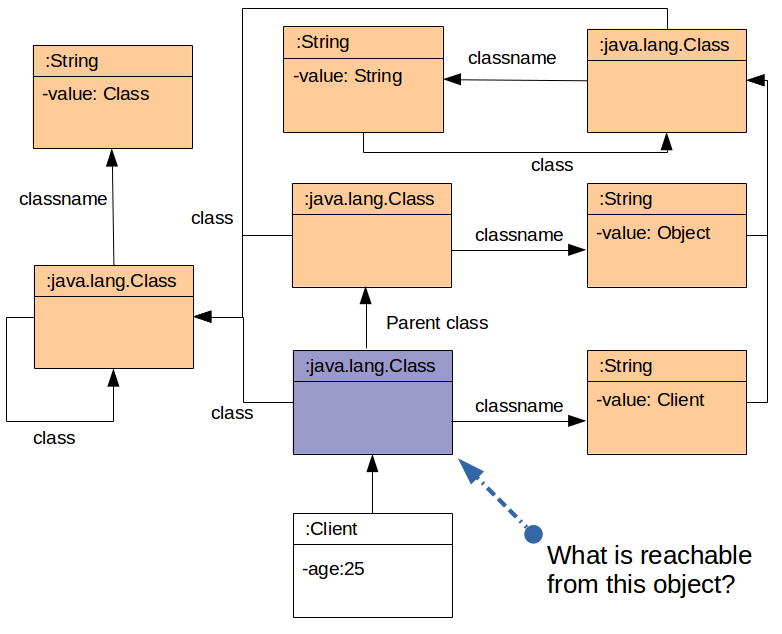
\includegraphics[scale=0.5]{./chapter6/fig/example1.png}
\caption{Objects reachable from the Client class. Observe that only one object is not reachable.}\label{fig:reachable-from-class-object}
\end{figure}

The aforementioned informal steps show what a profiler should be capable of doing:

\begin{itemize}
\item \textbf{Accessing meta-data of objects} such as the class of an object (\textit{java.lang.Class}), and the size of an object. 

\item \textbf{Accessing the value of attributes} is also helpful to filter out elements of the heap.

\item \textbf{Traversing references} is necessary because often some objects belong to a structure only because they are referenced by an object that is already a member.
\end{itemize}

To summarize, a function to determine whether an object is member of an structure may use: properties of the object itself, and properties about its relationships.

%\paragraph{Is there an instance of A making reference to an object of type B?}

%\paragraph{Length of each string, and number of objects referencing each string}

\paragraph{Nodes in each simply linked list}

In a second example, we want to calculate how many nodes has each simply linked list in the heap.
Figure~\ref{fig:simple_snapshot} shows a heap with two simply linked list and one double linked list.
The first list has three nodes while the second one has four; these are the values we want to obtain.

%Mostrar como hay patrones similares que se pueden detectar muchas estructuras
%Que entonces lo que se hace es describir el tipo de estructura con un paramtero adicional.

\begin{figure}[!ht]
\centering
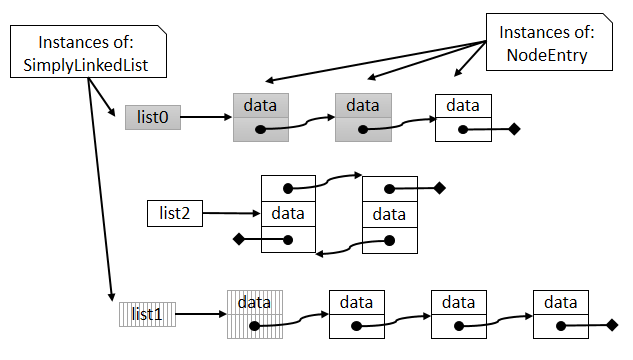
\includegraphics[width=0.65\linewidth]{chapter6/fig/lists}
\caption{Memory snapshot with three linked lists}
\label{fig:simple_snapshot}
\end{figure}


Informally, to compute such data a profiler must traverse the heap, checks whether an object's class is \textit{NodeEntry} (membership function), and increases a counter every time an instance is found (function to compute memory profile).
Unfortunately, these two steps are insufficient to correctly compute the fact that there exist two lists.
Indeed,  instead of the two values 3 and 4, a single value -- seven -- is obtained when this procedure is used.
The problem is that we have two structures instead of one, but using the aforementioned membership function it is impossible to know of which structure an instance of \textit{NodeEntry} is member of.
In other words, we need additional information to distinguish the two structures.

A method to solve this particular problem is to use the following recursive membership function: an object is member of a structure $S$ if it is an instance of \textit{NodeEntry} and it is being referenced by a member of $S$.
For the non-recursive case, we can see how each simply linked list starts with an instance of \textit{SimplyLinkedList}.
This is easily represented with a parametrized and recursive membership function:

\[
	f_{head}\left(O\right) = 
	\begin{cases}
		head = O & \quad O \; is \; \operatorname{SimplyLinkedList} \\
		\exists {x \in \operatorname{Objects}}, \quad x \operatorname{references} o \wedge f_{head}\left(x\right) & \quad O \; is \; \operatorname{NodeEntry} \\
		\operatorname{false} & \quad \operatorname{otherwise} \\
	\end{cases}
\]

The parameter $\textit{head}$ represents the structure of interest, and it is an instance of \textit{SimplyLinkedList}.
In this example, we have two functions, in which only the parameter varies, because there are two instances of class \textit{SimplyLinkedList}.
Similarly, we need two counters to store the number of nodes while we are traversing the graph of objects; once again, they (and the function to compute their values) are parametrized by the $head$ of the list.
Figure~\ref{fig:simple_snapshot} depicts a snapshot in time of the heap while it is being explored;
the shaded nodes are those that were already explored.

This example shows that in defining memory profilers, we often need the capacity for:

\begin{itemize}
\item Using the same functions for many structures, varying only some parameters. This is necessary for both membership functions and to compute the memory profile.

\item Identifying structures in the heap by using a parameter. For instance, in this example, we know that there are two structures because there are two instances of class \textit{SimplyLinkedList}.
\end{itemize}

To summarize, we are frequently interested in calculating values for many structures that have the same ``characteristics''; this is what we call \textit{structure type}.
To identify such structures we use a \textit{parameter}; the process of associating a particular parameter value to a structure type is done by a \textit{factory of structures}. 

\section{Metalanguage to define custom memory profilers}\label{sec:approach}

In this chapter, we propose a tool to create custom memory profilers for MRTEs.
We are interested on easing the task of defining new profilers without sacrificing their performance regarding CPU consumption.
This section presents our approach, a metalanguage to define custom memory profilers in MRTEs.
First, we present a global view of how our approach is used to support resource-aware programming, and how it integrates in a production environments (see Section~\ref{sec:dsl-global-architecture}).
Afterwards, the abstract syntax of this metalanguage is discussed; we present it using a metamodel of its main concepts as well as some snips of code in a concrete syntax to ease the presentation (see Subsection~\ref{sec:abstract-syntax}).
This concrete syntax is then presented in Subsection~\ref{sec:concrete-syntax}, followed by both the operational (evaluation) and translational semantic of the language (see Subsections~\ref{sec:operational-semantic} and~\ref{sec:translational-semantic}).
The section ends in Subsection~\ref{sec:dsl-usage-examples} by presenting some examples of how to use the language.

%Keeping the profiler's overhead as low as possible is of utmost importance for us because lightweight profilers can be use both during the development phase and during the application execution in a production environment.
%To reach this goal, we propose a Domain Specific Language (DSL) and its code generator which aims at describing and generating efficient online memory profilers. 

%We next present the syntax, semantics and usage examples of our domain-specific language.


\subsection{Global Architecture}\label{sec:dsl-global-architecture}

The global architecture of our approach is shown in Figure~\ref{fig:dsl-global-view}.
Since our goal is to support resource-aware programming, in this architecture, an application is able to collect data on its own memory consumption.
To provide this feature, we add a layer (data collection layer) to MRTEs to take care of: 

\begin{itemize}
\item Providing a set of interfaces to the memory profilers for collecting meta-data of objects in the heap, mechanisms to iterate over such objects, and to read the value of their fields.

\item Providing a set of interface for accessing memory profilers from the applications.
In other words, an application may trigger the execution of a memory profiler, and it can analyze the values compute by the profiler.

\item Supporting dynamic loading of memory profilers.
This is helpful in production environment for loading new dynamic analysis tools without having to stop the MRTE.
\end{itemize}

\begin{figure}[!ht]
\centering
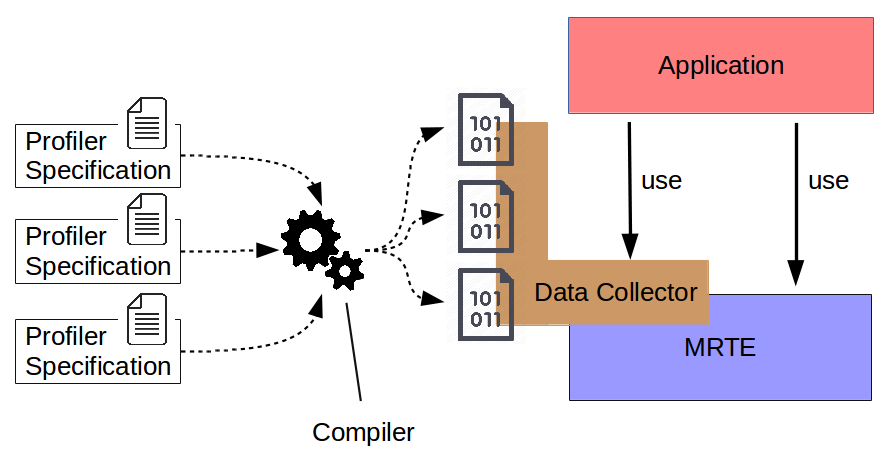
\includegraphics[scale=0.4]{./chapter6/fig/global-view.png}
\caption{Global view of the system. In this case, three memory profilers are defined.}\label{fig:dsl-global-view}
\end{figure}

In Figure~\ref{fig:dsl-global-view}, three memory profilers are plugged to the data collection layer.
The exact mechanism to collect raw data from the MRTE, as well as the mechanisms to dynamically load profilers, are platform specific.

A memory profilers can be handcrafted and plugged in this architecture; this is, nevertheless, error-prone.
Instead, we favor a generative approach where profilers are written using a metalanguage that hides low-level details.
A compiler is then used to transform such definitions into a binary form that can be executed in the runtime environment.
It is also in charge of providing interoperability between the data format provided by low-level facilities of the MRTE, and the high-level data format expected by applications running on top of such execution environments. 

\subsection{Abstract Syntax}\label{sec:abstract-syntax}

The metamodel shown in Figure~\ref{fig:as} describes the abstract syntax of our DSL.
The main concept of this metamodel is a \textit{CustomProfiler} which is composed of \textit{UserDefined} types and a \textit{StructureFactory}.
The concepts related to \textit{UserDefined} types are shown on the left part of the metamodel, while the right part describes the \textit{StructureFactory} which represents both the set of  structures to identify and the value to compute on these structures.

\subsubsection{User-defined types}
In addition to various \textit{BasicTypes} such as \textit{Integer}, \textit{String} and \textit{Boolean}, the language supports the definition of both \textit{Records} and \textit{Lists}.
As expected, a \textit{record} contains \textit{fields} to hold values of previously defined types.
Likewise, a \textit{list} refer to a \textit{base type}; hence all the members of a list must be of the same type.
In a custom profiler, \textit{UserDefined} types can be composed in arbitrary ways as long as no type contains a recursive declaration.
We can formalize such a constrain using OCL (Object Constraint Language~\footnote{\url{http://www.omg.org/spec/OCL/}}):

\begin{lstlisting}[escapeinside={(*}{*)},
label=fig:membership,
language=OCL1
]
context Record inv: 
   not fields->oclAsSet()->closure(t)->exists(t | t = self)

context List inv:
   not baseType->oclAsSet()->closure(t)->exists(t | t = self)
\end{lstlisting} 

A \textit{List} has operations to manipulate any value which represent a list.
Figure~\ref{fig:as} shows a subset of these operations.
In general, these operations correspond to the set of \textit{standard} operations of any implementation of the list data type.

\subsubsection{Defining structures to profile}
Defining the \textit{StructureFactory} is the core of writing a custom profiler.
A \textit{StructureFactory} contains an \textit{Expression} through the \textit{instances} relationship which indicates a pattern to identify structures in the memory heap.
Notice that a single instance of \textit{StructureFactory} creates many data structures in memory; thus the \textit{Expression} corresponds to a list indicating that a new structure must be instantiated for each element of the list.
Forcing the \textit{Expression} to be a \textit{List} can be easily formalized using OCL:

\begin{lstlisting}[escapeinside={(*}{*)}, label=fig:instances, language=OCL1]
context StructureFactory inv: instances.type.oclIsTypeOf(List)
\end{lstlisting}

Defining a new \textit{StructureFactory} implies defining its \textit{type} which is an instance of \textit{StructureType}.
This concept describes the mechanism used to populate, out of objects, a structure and its information.
In short, each structure in memory instanciated through a \textit{StructureFactory} has a type \textit{StructureType}.
For example, we may be interested in finding all the \textit{SimplyLinkedList} in the memory snapshot depicted in Figure~\ref{fig:simple_snapshot}.
In such a case, there are two \textit{SimplyLinkedList}, but we only need one mechanism to identify them because they have the same pattern in memory. 

\begin{figure*}
\centering
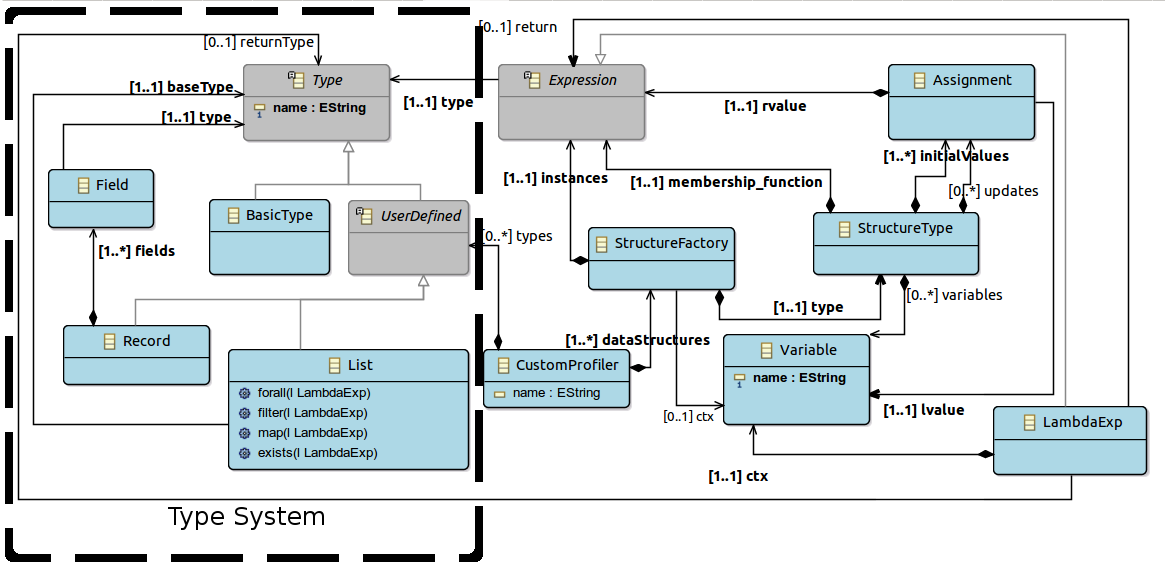
\includegraphics[width=0.87\linewidth]{chapter6/fig/AS}
\caption{Custom profiler Metamodel}
\label{fig:as}
\end{figure*}


A \textit{StructureType} is composed of \textit{Assignments} that are used as \textit{initialValues} for each \textit{Variable} holding information - similar to a constructor in object-oriented programming.
Once a new structure is created, the \textit{Assignments} are executed to assign the initial value of each \textit{Variable}.
Observe that \textit{variables} do not refer to a \textit{Type}.
Our DSL is strongly typed and the \textit{type} of each user-defined variable is inferred from its initial value.
Nevertheless, there is a built-in variable in each \textit{StructureType} that is only accessible during initialization.
Its type is predetermined as part of the language specification.
We force the use of the proper type using OCL:

\begin{lstlisting}[escapeinside={(*}{*)}, label=fig:instances, language=OCL1]
context StructureType inv:  initialValues->exists(a: Assignment | 
     a.lvalue.name = 'initialObjects' and a.rvalue.type.oclIsTypeOf(List)
   ) 
\end{lstlisting}

In addition, a \textit{StructureType} contains a boolean \textit{expression} which is the \textit{membership function} used to decide whether an object should be included in the structure instance.
Finally, it also contains a set of \textit{Assignments} to update the value of each \textit{variable} every time a new object is included in the structure.
This set of \textit{Assignments} is used to compute the actual value of the memory profile.
The major constraint regarding these \textit{updates} is that they must refer to already initialized \textit{variables} and the new assigned values must match the previous types.
We formalize such a constrain using OCL:

\begin{lstlisting}[escapeinside={(*}{*)}, label=fig:lvalue, language=OCL1]
context StructureType inv:  updates->forAll(a: Assignament | 
    self.initialValues->exists(aa : Assignament | 
       aa.lvalue = a.lvalue and aa.rvalue.type = a.rvalue.type
     ))
\end{lstlisting}

In our DSL, \textit{expressions} play a big role.
For the sake of readability, Figure~\ref{fig:as} only shows a couple of concepts related to them.
However, it is noteworthy that, in addition to \textit{arithmetic}, \textit{boolean} and \textit{literals} for basic types, the language includes lambda expressions, literal for records and lists.
Moreover, the language defines \textit{built-in rvalues} which are nothing but expressions initialized by the runtime within a specific scope.
Instead of being user-defined, the types of these expressions are also defined by the runtime.
There are two types of \textit{built-in rvalues}, target independent and dependent.
Among the firsts, we have the list of  \textit{objects}, a reference to the \textit{current data structure} and a reference to the \textit{current object}.
Target dependent \textit{rvalues} in Java include the list of \textit{loaded classes} and the list of \textit{threads}.
The precise meaning of these \textit{rvalues} as well as their scopes are precisely discussed in sections~\ref{sec:concrete-syntax}, ~\ref{sec:semantic} and~\ref{sec:implementation} along the concrete syntax, the language semantic and the tooling support.

Finally, if we use the memory snapshot depicted in Figure~\ref{fig:simple_snapshot}, calculating the number of nodes belonging to a specific \textit{SimplyLinkedList} is an example that illustrates the language's concepts.
To solve this problem we can instantiate the metamodel of our DSL as follow:
\begin{itemize}
\item Define a \textit{StructureFactory} in which the \textit{instances} property is a list which contains the objects \textit{list0} and \textit{list1}.
\item Instantiate a \textit{StructureType} where the built-in variable \textit{initialObjects} receives as value a list with one member - list0 or list1.
      The other properties of this \textit{StructureType} instance are detailed in the next steps: 
      \begin{enumerate}
      \item Define a variable \textit{n} with initial value zero.
      \item Define a membership function which return true if an object is instance of \textit{NodeEntry} and it is referenced by an object for which the membership function also return true. Observe how this recursive function returns true for each element in \textit{list0} because the initial object's list contains object \textit{list0}. 
      \item Update the variable \textit{n} by increasing its value by one.
      \end{enumerate}  
\end{itemize}
Further details about this example are discussed in the next section.

\subsection{Concrete Syntax}\label{sec:concrete-syntax}

A textual concrete syntax has been defined for our DSL allowing the domain expert to define a custom memory profiler using a text editor.
A high-level view of the grammar for this textual representation is depicted in Figure~\ref{fig:dsl-grammar}.
As can be seen, the rules that represent expressions make such a grammar ambiguous, we decided to use this form for the sake of the presentation.
However, a complete LL(*) grammar~\cite{Parr:2011:LFA:1993498.1993548} is presented hereafter in Annex~\ref{anx:grammar}.
One interesting aspect of this concrete language is its relative verbosity.
For instance, it uses very explicit keywords such as ``create structure foreach'', ``constructor'', and ``membership''.


%\setlength{\grammarparsep}{20pt plus 1pt minus 1pt}
{
\scriptsize
\begin{figure}[!ht]
\begin{mdframed}[outermargin=0.2cm, innermargin=0.5cm]

\newcommand{\grule}[1]{\hfill{\scriptsize (#1)}}
\setlength{\grammarindent}{5em}
\begin{grammar}

<program> ::= <types> <structures> \grule{1}

<types> ::= <type> <types> | <empty> \grule{2, 3}

<type> ::= <id> `:' `table-of' <id> | <id> `:' `struct' `{' <fields> `}' \grule{4, 5}

<fields> ::= <id> `:' <id> <fields> | <id> `:' <id> \grule{6, 7}

<structures> ::= <struct-factory> <structures> | <struct-factory> \grule{8, 9}

<struct-factory> ::= `create structure foreach' <id>`:'<e> `using' <body> \grule{10}

%<Header> ::= `create structure foreach' <id>`:'<expr>

<body> ::= `constructor' <s> `membership' <expr> `updates' <s> \grule{11}

%<constructor> ::=  \grule{12}

%<membership> ::= 

%<updates> ::= \grule{13}

<s> ::= <a> <s> | <empty> \grule{12}

<a> ::= <id> `=' <e>  \grule{13} 

<e> ::= <e> <binary-op> <e> | <unary-op> <e> \grule{14, 15}
\alt <e> `in' <id> | <e> `is' <id> \grule{16, 17}
\alt <e> `.' <id> `(' <expr-list> `)' \grule{18}
%\alt <e> `.' <id> `(' `[' <id> `|' <s> `]' `)' \grule{19}
\alt <e> `.' <id>                              \grule{20}
\alt `#[' <expr-list> `]' | `struct' <id> `{' <expr-list> `}' \grule{21, 22}
\alt <int-literal> | <string-literal> | <bool-literal> \grule{23, 24, 25}
\alt <id> | `(' <e> `)' \grule{26, 27}

<expr-list> ::= <e> `,' <expr-list> | `[' <id> `|' <s> `]' `,' <expr-list> | <empty>  \grule{28}

<binary-op> ::= `+' | `*' | `-' | `/' | `and' | `or'

<unary-op> ::= `-' | `not'

\end{grammar}
\end{mdframed}
\caption{Concrete grammar of the language. For the sake of clarity, we are using an ambiguous grammar to describe the expression language.} \label{fig:dsl-grammar}
\end{figure}
}

As an example, the next listing shows how to compute the length of each \textit{SimplyLinkedList} in the memory snapshot depicted in Figure~\ref{fig:simple_snapshot}.
The mechanism is based on counting the number of \textit{NodeEntry} referenced by the \textit{SimplyLinkedList}.
Each \textit{NodeEntry} is used to wrap one element of data and to point to the next element.

\begin{lstlisting}[escapeinside={(*}{*)}, 
label=lst:listLengt, language=DSL2
]
create structure foreach e:objects.filter(l| l is SimplyLinkedList) using
  constructor
    initialObjects = #[e] // a list literal with one element: e
    n = 0
  membership (this is NodeEntry) and (referrer in this_structure)
  updates 
    n = n + 1
\end{lstlisting}

In the example, only one \textit{StructureFactory} is necessary.
In line 1, we define the list of structures we are interested in.
We do so by selecting instances of class \textit{SimplyLinkedList} as elements of the \textit{StructureFactory}.
Since there are two simply linked lists in the memory snapshot, we are going to build two structures.
Observe the usage of a built-in \textit{rvalue} named \textit{objects} which contains all the objects in memory.
The valid scope of this rvalue is in both the definition of the set of structures and the computation of the initial values.
Thereafter, lines 2-4 specify the initial values.
Line 3 in particular initializes the set of objects included in the structure.
Notice the usage of a list literal to include the object referenced by \textit{e}.
In the initialization scope, the rvalue \textit{e} is equal to one of the element within the list of structures - either \textit{list0} or \textit{list1}.

In line 5 we define the membership function, which is used to determine if an object is part of the structure.
There are four built-in rvalues during the evaluation of the function as well as during the update of the variables.
First, the value named \textit{this} is the current visited object. 
The \textit{membership} boolean \textit{expression} aims at determining if this object is part of the \textit{structure} or not. 
The value \textit{this\_structure} identifies the structure.
As our runtime profiler will traverse the graph of in memory objects following references between objects, the object through which we have reached the \textit{this} object is known as \textit{referrer}.
The last value, which is target dependent, is the kind of reference.
Operator \textbf{is} checks if \textit{this} is an instance of class \textit{NodeEntry}.
Likewise, operator \textbf{in} checks whether the \textit{referrer} is already a member of the structure.
Finally, line 7 updates the length of the list when an object is detected as member of the structure.

\subsection{Operational Semantics} \label{sec:operational-semantic}

\extracomment{TODO}{
\begin{enumerate}
\item Add notation
\item Fix the rule that calls a method with a lambda expression
\item Add the rule for the interpretation of a program
\item Discuss the inference rules
\end{enumerate}
}

\begin{figure}
\begin{mdframed}[innermargin=0.3cm, outermargin=0.3cm]

{
\footnotesize

\begin{tabular}{rcl}
$Bool(1)$ and $Bool(0)$ & & \parbox{8cm}{Values  $true$ and $false$.}\\
& & \\
$ E $ & \parbox[t]{0.7cm}{} & \parbox{8cm}{Describes a mapping from \textit{identifiers} to \textit{locations}. We use $id \mapsto l$ to represent a member of the mapping} \\ 
& & \\
$ S $ & & \parbox[t]{8cm}{Describes a mapping from \textit{locations} to \textit{values}. Informally, it can be seen as the storage. We use $l \mapsto v$ to represent a member of the a mapping.} \\ 
& &  \\
$ C $ & & \parbox[t]{8cm}{Describes a mapping from \textit{values} to \textit{structures}. We use $v \mapsto s$ to represent a member of the mapping.} \\ 
& & \\
$\left[ k_1 \mapsto v_2, \dots, k_n \mapsto v_n \right]$ & & \parbox[t]{8cm}{Describes a mapping by enumerating its members.} \\ 
& & \\
$S\left[ v_i/k_i \right]$ & & \parbox[t]{8cm}{Describes a new mapping where $S\left[ v_i/k_i \right](k_j) = S(k_j)$ if $k_i \ne k_j $, $S\left[ v_i/k_i \right](k_j) = v_i$ otherwise. } \\
& &  \\
$M \overset{\operatorname{val\_of}}{\vdash} k \mapsto v$ & & \parbox[t]{8cm}{A set of auxiliary rules to compute the value $v$ that is associated to the key $k$ in the mapping $M$.} \\ 
& &  \\
$C \overset{\operatorname{contains}}{\vdash} v \mapsto s \Rightarrow r$ & & \parbox[t]{8cm}{A set of auxiliary rules to determine whether the value of $v$ is mapped to $s$ in $C$, which is always a mapping from  \textit{values} to \textit{structures}. $r$ is a boolean value. } \\
& &  \\
$\lVert E,S, id, e\rVert$ & & \parbox[t]{8cm}{Describe a closure, $E,S$ represents the state, $id$ is the identifier used as parameter of the closure, and $e$ is the expression to evaluate.} \\ 
& & \\
$T(a_1 \mapsto l_1, \dots, a_n \mapsto l_n)$ & & \parbox[t]{8cm}{A generic value in the language. $T$ is its type, and a mapping from attributes $a_i$ to their respective locations $l_i$. Sometime, we use $\mathbb{A}$ to represent the mapping. There are shorthands for special cases: $Bool(1)$, $Bool(0)$, $Int(n)$ which is the integer $n$, and $String(w)$ which is the string $w$. In addition, the value $table(l_1,\dots,l_n)$ denotes a table; in this case, $l_i$ is the location in storage of the \textit{i-th} element of the table. } \\ 
& & \\
$\langle T, P, a_1 \mapsto T_1, \dots, a_n \mapsto T_n \rangle$ & & \parbox[t]{8cm}{Describe a type with identifier $T$. The description contains the parent type $P$ (which has the same structure), and its attributes $a_i \mapsto T_i$. } \\
& & \\ 
$\overset{\operatorname{subtype}}{\vdash} S, P \Rightarrow r$ & & \parbox[t]{8cm}{A set of auxiliaries rules to determine whether type $S$ is a subtype of $P$. $r$ is a boolean value.} 
\end{tabular} 

}

\end{mdframed}
\caption{Notation used in the operational semantic}\label{fig:notation-for-operational-semantic}
\end{figure}

\renewcommand{\inference}[3][]{%
  \begin{array}[b]{@{}c@{}c@{}}
    \smash{\raisebox{-.5\normalbaselineskip}{{\scriptsize #1}}} & 
      \begin{array}[b]{l}
        #2
      \end{array} \\
      \cline{2-2}
    & \begin{array}[t]{c}
        #3
      \end{array}
  \end{array}
}

\mathlig{->}{\mapsto}
\mathlig{|-}{\vdash}
\mathlig{=>}{\Rightarrow}
\mathlig{"}{\;\;\;}

\mathligson

% classics
{
\footnotesize
\[
% true
\textnormal{{\scriptsize It(25):}}\; E, S\vdash\operatorname{true}\Rightarrow Bool(1),S
\quad\quad
% false
\textnormal{{\scriptsize It(25):}}\; E, S\vdash\operatorname{false}\Rightarrow Bool(0),S
\]

\[
% integers
\textnormal{{\scriptsize It(23):}}\; E, S\vdash\operatorname{Integer}\; N\Rightarrow Int(N),S
\quad\quad
% strings
\textnormal{{\scriptsize It(24):}}\; E, S\vdash\operatorname{String}\; w\Rightarrow String(w),S
\]

% lambda expressions
\[
\textnormal{{\scriptsize It(19):}}\; E, S\vdash \left[id \vert e \right] \Rightarrow \lVert E,S, id, e\rVert,S
\]

\[
% id
\inference[It(26):]{
E\overset{val\_of}{|-}id->l_{id} "" S\overset{val\_of}{|-}l_{id}->v
%v = S \; E \; id
}{E, S|-id=>v,S}
\quad\quad
% (e) 
\inference[It(27):]{
E, S|-e=>v,S_1
}
{E, S|-(e)=>v,S_1}
\]

\[
% unary operators
\inference[It(17b):]{
E, S|-e_0=>v_0,S_1
}{E, S|-\operatorname{op}e_0=>\operatorname{op}v_0,S_1}
\quad\quad
% binary operators
\inference[It(17a):]{
E, S|-e_0=>v_0,S_1 "" E, S_1|-e_1=>v_1,S_2
}{E, S|-e_0\operatorname{op}e_1=>v_0\operatorname{op}v_1,S_2}
\]

\[
% in operator
\inference[It(17c):]{
C, E, S|-e_0=>v_0,S_1 "" C \overset {in} {|-} v_0->id =>v
%v = v_0->id \in C? Bool(1):Bool(0)
}{C, E, S|-e_0 \; in \; id=>v,S_1}
\quad\quad
\]

\[
% is operators
\inference[It(17d):]{
E, S|-e_0=>X(\mathbb{A}),S_1 "" \overset{subtype}{|-} X, T \Rightarrow v
}{E, S|-e_0\; \operatorname{is} \; T:v,S_1}
\]

\[
% assignment
\inference[It(16):]
{
E,S|-e_0=>v_0,S_1 "" E\overset{val\_of}{|-}id->l_{id}
%l_{id} = E(id) \\
%S_2 = 
}
{E, S|-id = e_0=>v_0, S_1[v_0/l_{id}]}
\quad\quad
% statements
\inference[It(14)]
{
E, S|-a=>v_a,S_1 "" E, S_1|-s=>v,S_2
}
{E, S|-a\;s=>v,S_2}
\]

\[
% struct literal
\inference[It(22):]
{
E,S|-e_1=>v_1,S_1 \\
\vdots \\
E,S_{n-1}|-e_n=>v_n,S_n \\
\operatorname{class}(T)=(a_1->T_1, \dots, a_n->T_n) \\  % take the fields of the object
l_i = \operatorname{newloc}(S_n) \; for \; i = 1 \dots n \\
v=T(a_1->l_1, \dots, a_n->l_n) \\ % assign locations to fields
S_f = S_n[v_1/l_1, \dots, v_n/l_n]
}
{E, S|-struct\;T\;\{ e_1, \ldots, e_n \}:v,S_f}
\quad\quad
% list literal
\inference[It(21):]
{
E,S|-e_1=>v_1,S_1 \\
\quad \vdots \\
E,S_{n-1}|-e_n=>v_n,S_n \\
l_i = \operatorname{newloc}(S_n) \; for \; i = 1 \dots n \\
v=\operatorname{table}(l_1, \dots, l_n) \\
S_f = S_n[v_1/l_1, \dots, v_n/l_n]
}
{E, S|-\#[e_1, \dots, e_n]:v,S_f}
\]

\[
% accessing field
\inference[It(20):]{
E,S|-e=>X(\mathbb{A}),S_f "" \mathbb{A} \overset{val\_of}{|-} \textit{id} -> l_{\textit{id}} "" \mathbb{S} \overset{val\_of}{|-} l_{\textit{id}} -> v
%v0 = X(a_1->l_1, \dots, a_n->l_n) \\
%l_{id} = l_i \; where \; a_i = id \\
%v = S_1(l_{\textit{id}}) \\
}
{E,S|-e.\textit{id}=>v,S_f}
\]

\[
% calling method
\inference[It(18):]{
E,S|-e_0=>X(\mathbb{A}),S_0 \\
E,S_0|-e_1=>v_1,S_1 \\
""" \vdots \\
E,S_{n-1}|-e_n=>v_n,S_n \\
\operatorname{impl}(X,f) = (x_1, \dots, x_n, f_{body}) \\
l_{x_i} = \operatorname{newloc}(S_{n+1}) \; for \; i = 1 \dots n \\
\mathbb{A}[l_{x_1}/x_1, \dots, l_{x_n}/x_n],S_n[v_1/l_{x_1}, \dots, v_n/l_{x_n}]|-f_{body}:v,S_f
}
{E,S|-e_0.f(e_1, \dots, e_n):v,S_f}
\]

% news

%\[
%% lambda expressions
%\inference[It(19) mal]{
%v = \lVert E, \left[ id | s \right] \rVert " a " v
%}{
%E,S|-[id|s]:v,S
%}
%\quad\quad
%% calling function with lambda expression
%\inference[It(19) mal]{
%E,S|-e_0:v_0,S_1 \\
%v_0 = X(a_1=l_1, \dots, a_m=l_m) \\
%\operatorname{impl}(X,f) = (x_1, f_{body}) \\
%l_{x_1} = \operatorname{newloc}(S_1) \\
%E' = [a_1:l_1, \dots, a_m:l_m][l_{x_1}/x_1] \\
%v_1 = \operatorname{Clousure}(E, \left[ id | s \right]) \\
%v_0, E', S_1[v_1/l_{x_1}]|-f_{body}:v,S_f 
%}{
%E,S|-e_0.f\left( \left[ id | s \right] \right):v,S_f
%}
%\]
%
}



\mathligsoff

\subsection{Translational Semantics}\label{sec:translational-semantic}

An instance of our metamodel is compiled into a custom memory profiler.
This compilation produces a library written in \textit{C++} which is in charge of collecting the desired information from the runtime environment.
The generated source code has two parts.
First, for each \textit{StructureType} in the model, the compiler generates a subclass of \textit{AbstractStructureType} which is shown below.
Every subclass contains attributes to store the variables used in the associated \textit{StructureType}.
In the listing below, the class \textit{Context} holds the built-in values we mention in the previous section.
\begin{lstlisting}[language=C++, frame=L,
numbers=left,
numberstyle=\color{black}\scriptsize,xleftmargin=2\parindent]
class AbstractStructureType {
public:
	void initialize(Context& ctx) = 0;
	bool membership(Context& ctx) = 0;
	void update(Context& ctx) = 0;
}
\end{lstlisting}

The second part of the generated code is formed by a set of initialization routines, one for each \textit{StructureFactory}.
Each routine creates a list of structures with a specific \textit{AbstractStructureType} - the \textit{T} parameter in the listing.
Formally, the signature and behavior of these routines are as follow:
\begin{lstlisting}[language=C++, frame=L,
numbers=left,
numberstyle=\color{black}\scriptsize,xleftmargin=2\parindent]
template <typename T> void
[name](Context& ctx, std::vector<AbstractStructureType*>& s){
  for (Object obj : ctx.instances) {
    AbstractStructureType* ns = new T();
    ctx.e = obj;
    ns->initialize(ctx);
    s.add(ns); // not valid in the STL, but simpler to read
  }
}
\end{lstlisting}
An important concern during the transformation lies on efficiently mapping our concepts to \textit{C++} concepts.
Moreover, since each target platform provides facilities to get metadata regarding the objects in memory, using such facilities efficiently is specially important in order to reduce the performance overhead due to profiling.

The final profiler is built using both the generated code and a template algorithm.
The template is target dependent, but in general we use the underline target facilities to collect meta-data, access fields in certain steps, traverse the objects in memory and also to populate the built-in rvalues.
A simplified version of the used algorithm is shown below:
\begin{lstlisting}[escapeinside={(*}{*)},
label=lst:template, language=AlgLang, frame=L,
numbers=left,
numberstyle=\color{black}\scriptsize, xleftmargin=2\parindent]
values:
   structures: vector<AbstractStructureType*>
routine:
   foreach (initialization rountine (*$R_i$*) associated to a StructureFactory)
      create context
	  call (*$R_i$*)(context, structures)
   foreach (r: references among objects)
      if (r.target has no membership)
         create context // context.this = r.target
         S = structures.findfirst(s | s.membership(context))
         make context.this a member of S
         S.update(context)
   return structures 
\end{lstlisting}
There are two loops in the algorithm. 
The former loop is in charge of creating the set of structures the program is intended to collect information about.
The creation of the context in line 5 depends on the target platform.
It basically creates values such as the list of objects in memory or the list of loaded classes.
The latter loop traverses all the references among objects in memory.
During each iteration, the algorithm finds the first structure for which the membership function is true.
Notice that we only select the first because for some memory accounting problems, it is too hard to define a membership functions that build disjoints structures~\cite{dsn/09/geoffray/ijvm,Attouchi:2014:MMM:2602458.2602467}.
Thereafter, the information for such a structure is updated.

%The complete execution of a program in our language is as follow. Subgraph instances are initialized using listing~\ref{onInitialization}.
%Afterward, all the references in the graph of objects are traversed running listing~\ref{lst:onNodeFoundData}.
%The output data for all subgraph instances has been collected after all the references are traversed once.

%Finally, in listings~\ref{lst:onNodeFound},~\ref{lst:onNodeFoundData} and~\ref{onInitialization} we use built-in properties that are defined by the user.
%These properties must have access to some data describing the content of the memory in order to successfully identify subgraphs and calculate output values.
%Such data is wrapped in what we call execution context.
%In our DSL there are two different execution contexts: \textit{global context} and \textit{local context}.
%The former includes built-in values such as: i) lists of \textit{objects}, \textit{threads}, \textit{classes}, etc. , and ii) a value called \textit{Entity} representing a subgraph instance.
%The latter only contains the object \textit{THIS} which is being visited, a label of the reference representing its type, \textit{REFERRER} which is the object referencing the visited and again the \textit{Entity} value.
%The \textit{global context} is available in listing~\ref{onInitialization} while the \textit{local context} is available in both listings~\ref{lst:onNodeFound} and~\ref{lst:onNodeFoundData}.

\subsection{Language Usage} \label{sec:dsl-usage-examples}

\extracomment{FIX}{Improve explanations, add a caption to each listing, improve the style of each listing}

There are several possibilities for using our DSL in the various stage of an application lifecycle.
These include checking: local data structure invariants, reachability properties, memory consumption properties and combinations of those.
Below, we show some examples to highlight possible usage of our language. 
 
The first example shows how to assert the existence of a value satisfying some properties, independently of which object contains it. 
The result is obtained through the use of a filter on the list of objects.
The assertion successes if the heap contains an object with an attribute named $data$ with a value comprised between $3.141$ and $3.142$.

\begin{lstlisting}[escapeinside={(*}{*)},
%label=assertion, 
language=DSL2]
create structure foreach e:#["whole-jvm"] using
  constructor
    initialObjects = #[]
    existValue = false
  membership true
  updates 
    existValue = existValue or (this.data > 3.141 and this.data < 3.142)
\end{lstlisting}

The goal of next listing is to detect a bug identified in~\cite{Aftandilian:2009:GAU:1543135.1542503}.
This listing aims at finding if there exists an instance of the class $Order$
with the value of its field $field$ being equal to $specialValue$.
This technique is used to detect if one object has been garbage collected or if someone still holds a reference on it preventing its garbage collection.

\begin{lstlisting}[escapeinside={(*}{*)},
%caption=Detecting a knwon bug in pseudojbb., 
%label=pseudojbb,
%float=!h,
language=DSL2]
create structure foreach e:#["whole-jvm"] using
  constructor
	initialObjects = #[]
	fault = false
  membership  true
  updates
    fault = fault or (this is Order and this.field = specialValue)
\end{lstlisting}

The next example computes a combination of reachability and memory consumption properties.
It calculates the number of objects, and their total memory consumption, that are reachable from the threads.
We can notice how the membership property discards those objects that are not referenced by an already included object.  

\begin{lstlisting}[escapeinside={(*}{*)},
caption={Calculating objects reachables from threads},
label=kevoreeaccounting,
%float=!h,
language=DSL2]
create structure foreach e:#["whole-jvm"] using
  constructor
    initialObjects = threads
    nbObjects = 0 
    nbSize = 0 
  membership ( this in None and referrer in this_structure )
  updates 
    nbObjects = nbObjects + 1  
    nbSize = nbSize + this.size
\end{lstlisting}

We can also express complex structures in memory.
For instance, to find the consumption of K3-Al object namely \textit{K3Object} as described in Section~\ref{sec:chapter2-introduction}, we must find all instances of \textit{HashMap.Entry} that have \textit{K3Object} as the \textit{key}. These entries should be added to the consumption of the object \textit{K3Object} as well as all the objects reachable from the \textit{HashMap.Entry.value}.
To come out with this solution a good understanding of how K3-Al implements aspects is required.
The rationale here is that K3-Al stores the state of aspects in a separate HashMap, using as key the object to be aspectized.

\begin{lstlisting}[escapeinside={(*}{*)},
%caption=Computing the consumption of each K3-Al Object along with its aspects., 
%label=k3,
%float=!h, 
language=DSL2]
create structure foreach e:objects(*{.filter}*)([it|it is K3Object]) using
  constructor
    initialObjects = #[e]
    nbSize = 0
  membership (referrer in this_structure and this in None ) or
    (this is HashMap.Entry and this.key in this_structure and 
      this.key is K3Object)
  updates
    nbSize = nbSize + 1
\end{lstlisting}

\section{Tooling}\label{sec:dsl-implementation}

To validate our approach, we have implemented a tool chain to ease the definition of custom memory profilers for Java-based systems.~\footnote{Available at: \url{https://github.com/intigonzalez/heapexplorer\_language}}
These profilers can be executed in any JVM as long as it provides support for the JVMTI.

In this section, we present tools built to support the definition of memory profilers using our language; this is done by taking into account how engineers in different roles may interact with these tools and with the resultant profilers.
Indeed, in dealing with memory profilers, we have to take into consideration the two usual roles -- developers of profilers and their users; after all, profilers built using our language are themselves software abstractions.
A developer must know how the target domain-specific abstractions are represented atop the JVM, and she also must have a clear understanding of how our language is executed.
On the contrary, users only need to be aware of the interface provided by our framework, and the structure of the data collected by a profiler.
In the rest of this section, we discuss details that are important to these roles.

Additionally, we present low-level details regarding how the language is implemented atop of the JMVTI.
The decision of implementing our approach by relying on JVMTI has advantages and disadvantages.
On the one hand, the obvious advantage lies on the portability of this solution, which makes it more valuable from a practical point of view.
On the other hand, building profilers on top of the JVMTI, instead of directly modifying the JVM, impacts the performance of the generated profilers and, unfortunately, hinders (in extreme case it even prevents) the implementation of some language constructs.
Nonetheless, it is our belief that guarantying profilers' portability should be of maximum priority.
Moreover, in writing this implementation, we have found that the limitations in the JVMTI preventing the construction of better profilers can be overcome with, at most, a few additions to the API.


\subsection{Developers of domain-specific abstractions}

%\extracomment{FIX}{I am fixing this section, you can continue in Section~\ref{sec:dsl-tooling-users}}

In our vision, developers of software libraries and component frameworks, as well as software language engineers may use our approach to  define customized memory profilers for the abstractions they create.
This is, in addition to delivering artifacts such as libraries, source code, simulators, text editors for DSLs, and compilers for these DSLs; engineers would also ship profilers to simplify the use of these abstractions.
For instance, the developers of the Spring framework~\footnote{\url{https://spring.io/}} may create a set of specific profilers to reduce the cost of maintaining applications written using the framework.
These profilers can serve as both internal tools to help in the development of abstractions, and mechanisms allowing users to better use abstractions.

Figure~\ref{fig:dsl-tooling-developer} summarizes the viewpoint of developers of domain-specific abstractions.
To write a profiler, they use knowledge about the abstraction and the tool chain to generate the executable profiler. 
Our implementation of the language is built using Xtext~\cite{Eysholdt:2010:XIY:1869542.1869625}; it provides a textual editor that is able to handle the proposed concrete syntax.
This editor provides syntax highlighting, error detection during editing, auto-completion, and compilation to native Java agents written in \textit{C++}.

\begin{figure}
\centering
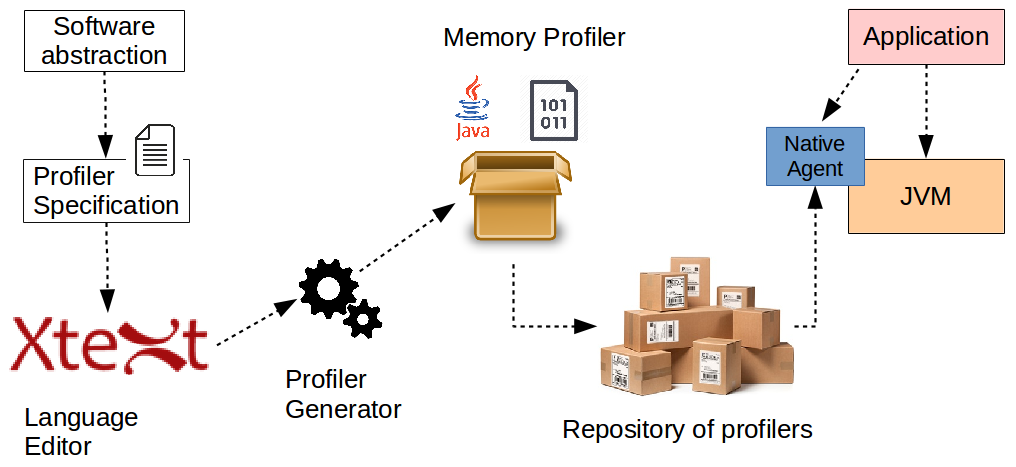
\includegraphics[scale=0.45]{./chapter6/fig/developer-profiler-view.png}
\caption{Viewpoint of developers. Memory profilers are built from the description of software abstractions.}\label{fig:dsl-tooling-developer}
\end{figure}

To perform low-level tasks related to memory profiling, we use \glslink{JVMTI}{JVMTI}~\footnote{\url{http://docs.oracle.com/javase/8/docs/platform/jvmti/jvmti.html}} and \glslink{JNI}{JNI}.
These APIs are used by both profilers and the core memory profiling library, so-called Native Agent in Figure~\ref{fig:dsl-tooling-developer}.
In this native agent, a \textit{plugins} system, which allows users to load/unload profiles without shutting down the JVM, is implemented.
Given a profiler definion, the compiler output is a package that contains a package with the native binary code for the profiler, and a Java library you can use to access the collected data using plain Java objects.

To reduce the overhead of profilers, developers must be aware of the details of the abstraction for which the profiler is being built, the semantic of our language, and the details of its implementation.
In particular, it is advisable reducing the usage of \textit{lists} and the evaluation of nested lambda expressions.
Likewise, heavily using the built-in rvalue \textit{objects} is specially discouraged because it can easily contains many elements.
It is also discouraged because, in order to reduce memory consumption, we rely on an iterator built on top of JVMTI operations that can be costly to use in terms of CPU time.

Finally, we added some built-in rvalues in this implementation because they are both useful in the context of Java and easy to obtain using the JVMTI.
These values are \textit{classes}, \textit{classloaders}, \textit{threads} and \textit{objects}; they are lists of anonymous built-in record types.
The relations among these types and their operations are depicted in Figure~\ref{fig:dsl-built-in-types}.

\begin{figure}
\centering
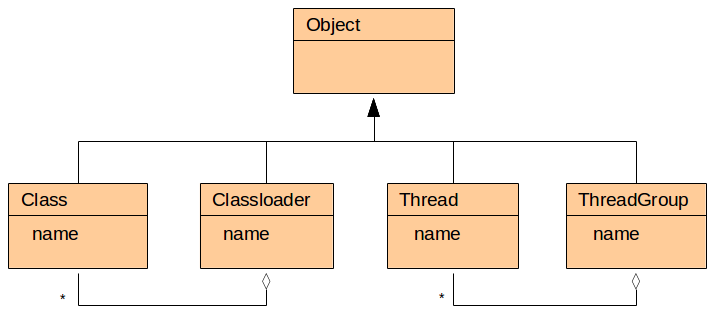
\includegraphics[scale=0.45]{./chapter6/fig/diagram-classes.png}
\caption{Viewpoint of developers. Memory profilers are built from the description of software abstractions.}\label{fig:dsl-built-in-types}
\end{figure}

%Indeed, the process of code generation is driven by the need of reducing the performance impact.
%In our implementation, we apply a set of platform dependent optimizations taking into account the profiler description.
%First, since a profiler does not always need built-in rvalues (e.g., \textit{threads}, \textit{threadgroups} and \textit{classes}, etc.), we selectively skip the construction of them.
%When possible, we also skip the construction of some structures (e.g., class of each object, its classloader, field names, etc.).

\subsection{Users of domain-specific abstractions} \label{sec:dsl-tooling-users}

We envision that a set of memory profilers can be shipped in addition to other ``classic'' deployment artifacts that users of a software abstraction receive. 
These profilers would support the use of the corresponding software abstraction.
For instance, an user who is relying on a new extension of the Xtend language to build a system, might use specific profilers written in our language to understand the memory consumption, and in general, the behavior of the system.

The generated profilers can be used in two different ways, either as development tools or as mechanisms to support resource awareness at runtime.
Due to the scope of this thesis, the reference implementation we provide is biased towards the second scenario, but it should be relatively simple to adapt it to support the software development process.
To access memory profilers, a JVM must be launched with a native Java agent loaded, and a library to collect profiling data in its classpath.
Once the application is running, it can trigger profiling by simple issuing a few method calls using the profiling API.
Figure~\ref{fig:user-profiling-library-view} illustrates the process of collecting memory profiles, the software components involved, and the APIs that must be used.
Observe how the profiling framework issues a call to a handler once it is done, a parameter contains the data computed.
These data are encoded in a \textit{list}, in which each elements correspond to the data computed for each identified structure in the heap.
%The problem is knowing the type and shape of each list element.

\begin{figure}[!b]
\centering
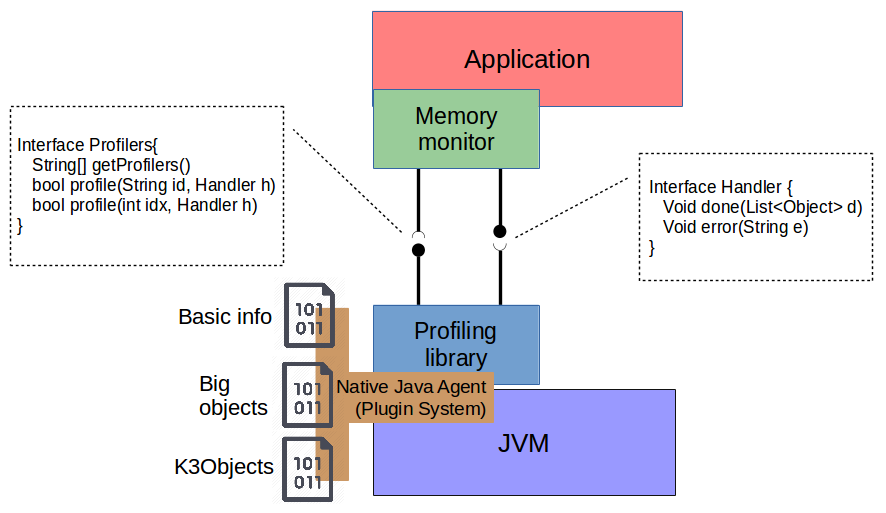
\includegraphics[scale=0.6]{./chapter6/fig/user-profiler-view.png}
\caption{Viewpoint of users. Memory profilers are black-boxes accessed through Java interfaces. Data collected is in the form of plain Java objects.}\label{fig:user-profiling-library-view}
\end{figure}

The output of a profiler is a list of Java objects containing the collected information; and the type of these objects depend on the profiler definition.
Indeed, as part of our implementation, the profiler generator creates a set of Java classes to represent the data collected in a form that is easy to digest at runtime by a Java application.
Once a profiler collects the information in an internal format, it populates a representation in Java using the Java Native Interface (JNI); the code to do so is also generated by the compiler of our language.
In Figure~\ref{fig:dsl-generated-java}, the classes generated for a profiler are shown.
Notice that a class is created for each \textit{record} declared, and also for each \textit{StructureType}.
It can be seen how `lists' are directly represented in Java by mean of generic Java lists.
The \textit{id} field in both \textit{MemoryProfile1} and \textit{MemoryProfile2} is the value used to parametrize each structure;
in this particular example, where two structures are identified, the value of \textit{MemoryProfile1.id} is ``lists'' and the value of \textit{MemoryProfile2.id} is ``otherObjects''.

Given the fact that the data computed by a profiler is returned as a list of objects, and their layout is unclear, the remaining problem is how to process such data; there are two options.
First, users can make the application code depend on the Java code created by the profiler generator.
In this way, your application has a new dependency, but you can profit from knowing at development time the types used in the code.
A second approach is using the reflection capabilities of Java to explore the data.
In the evaluation, we use such an approach to log the result of an arbitrary profiler, printing all the information it has computed.
Using reflection, it is also possible to build a user interface to explore the results in a customized way.  

\begin{figure}
\centering
\begin{minipage}[t]{0.60\linewidth}
\begin{lstlisting}[language=DSL2]
name "basic info" 

T : struct {
	classname : String
	size: int
}
create structeres for e:#["lists"]
using
	constructor
		initialObjects = #Object[]
		data1 = #T[];
	membership
		(this is String) or (this is Array)
	updates
		data1 = data.add(struct T { this.classname, this.size})
		
create structeres for e:#["otherObjects"]
using
	constructor
		initialObjects = #Object[]
		data2 = #T[];
	membership true
	updates
		data2 = data.add(struct T { this.classname, this.size})
\end{lstlisting}
\end{minipage}
\hspace{0.07\linewidth}
\begin{minipage}[t]{0.30\linewidth}
\begin{lstlisting}[language=java, frame=L, numbers=left,numberstyle=\color{black}\scriptsize]
class T {
	final String classname;
	final int size;
}

class MemoryProfile1 {
	final Object id;
	final List<T> data1;
}

class MemoryProfile2 {
	final Object id;
	final List<T> data2;
}
\end{lstlisting}
\end{minipage}
\caption{Representation of profiling data in Java, as users of profilers see it. Accessing these structures is useful to support resource awareness.} \label{fig:dsl-generated-java}
\end{figure}




%The process of code generation is driven by the need of reducing the performance impact.
%In general, there are two ways of optimizing the impact of the memory's analysis.
%First, we can apply platform dependent optimizations.
%The second option is to apply platform independent optimizations; for instance, simplifying the evaluation of each expression.
%In our implementation, we use both platform dependent and independent optimizations.
%
%A set of platform dependent optimizations we perform is related to the construction of the built-in values \textit{threads}, \textit{threadgroups}, \textit{classes}, etc. 
%Since not all memory analysis depends on such values, we selectively skip the construction of them.
%For instance, in listing~\ref{assertion} there is no need to compute any of such values as is also unnecessary to identified the class of each object.
%Extending this idea to other cases (e.g., class of each object, its classloader, field names, etc.) is straightforward.
%To implement these optimizations, we used a parametrized code template, so the code generate depends on the values of these parameters which we can tune to satisfy our needs.
%
%An other optimization we perform is related to the existence of collections as data type in our DSL.
%These collections can be potentially large, in particular, the \textit{objects} value is costly to compute and keep in memory.
%This fact combined with the usage of operations on collections such as \textit{map} and \textit{filter} may harm the performance of an analysis.
%That is why we devise two strategies to deal with collection values.
%User-defined and most built-in collections are kept in memory using linear space.
%On the contrary, we represent the built-in collection \textit{objects} as a generator.
%This representation is feasible because the mechanism provided by JVMTI to access the objects is based on callbacks.
%
%A last optimization is reducing the nodes of the graph that must be traversed
%As an illustration, we only produce code to explore primitive fields of each object, which are represented as leaf nodes in the graph, if there exist some expression accessing a field.
%
%As for platform independent optimizations, we mostly change the order in which boolean expressions are evaluated.
%We try to guarantee that subexpressions accessing collections and fields are evaluated as little as possible.
%
%The current implementation is limited in the number of optimization it applies.
%The main overhead reduction is achieved thanks to the execution model in which many paths of the graph are not traversed.
%Other benefits come from deciding at compilation time if some parts of the graph such as the leaf nodes must be explored or not.


\section{Discussion On Language Expressiveness}\label{sec:expressiveness}

In our DSL, the mechanism used to collect data is explicit to the user.
Hence, it is possible to estimate the overhead of a specific profiler.
In short, our DSL follows the imperative paradigm to obtain derived values.
On the contrary, most query languages provide a declarative style because it \textit{simplifies} writing new queries.

%Designing a domain specific language for memory analysis is a deliberate attempt to make explicit to the user what is the complexity of the analysis he tries to perform.
We acknowledge that our approach limits the kind of memory analysis that users can express.
First, it is not possible to recover all the information contained in the graph of live objects in linear time on the number of objects.
Second, an imperative style forces the users to understand the underlying execution model which is not required with declarative query languages.
Nonetheless, we claim that getting rid of some expressiveness is a trade-off worth considering in order to guarantee efficient memory analysis.
The empirical and theoretical evidence suggest that, in our DSL, \textit{reducing the capabilities to collect data} has a bigger impact on performance gain than \textit{generating efficient native code} to collect data.

At this point, it is worth noting why declarative approaches fail to deliver the adequate performance in production.
Listings~\ref{k3OQL} and~\ref{k3Cypher} show possible solutions, in OQL and Cypher/Neo4j, to the K3-Al example presented in section~\ref{sec:motivation}.
There are two aspects affecting the performance of this kind of queries.
We next discuss them.

\begin{lstlisting}[escapeinside={(*}{*)},caption={Using OQL to compute the consumption of each K3-Al object. Actually, this query cannot be executed in Eclipse Mat nor in VisualVM since they do not provide a full OQL implementation. }, label=k3OQL,float=!h, language=OQL]
SELECT id, sum(size) as s
FROM (
	SELECT
		e.key.@objectId AS id, 
		e.@usedHeapSize + e.value.@retainedHeapSize AS size
	FROM java.util.HashMap$Entry e
	WHERE (classof(e.key).@name = "K3Object")
	UNION ALL
	SELECT 
		k3.@objectId AS id, k3.@retainedHeapSize AS size 
	FROM K3Object k3
)
GROUP BY id
\end{lstlisting}

In the first place, many queries are intrinsically complex to answer.
For instance, it is known that answering SPARQL queries - which was used as inspiration for Cypher/Neo4j, is PSPACE-complete~\cite{Schmidt:2010:FSQ:1804669.1804675, Perez:2009:SCS:1567274.1567278}.
The performance of declarative queries for in production memory analysis is also affected by the nature of data we are exploring. 
Indeed, even if they can be executed efficiently, the optimization steps required are in most cases impossible to execute for the type of data we are considering - a graph of objects that constantly changes.
Often, these query optimizations require access to indexes, additional storage and multiples passes on the data~\cite{Elhemali:2007:ESS:1247480.1247598, Dageville:2002:SMM:1287369.1287454} that are not accessible on the graph of objects.
\begin{lstlisting}[escapeinside={(*}{*)},
caption={Using Cypher to compute the consumption of each K3-A1 object.}, label=k3Cypher,float=!h, language=CYPHER]
MATCH 
	(key:K3Object)<-[:key]-(entry:HashMap$Entry)-[:value]->value
WITH entry, key, value
MATCH 
	key-[:1..1]->fieldK
WITH entry, key, value, fieldK
MATCH 
	value-[:1..1]->fieldV
RETURN key, entry.size + key.size + fieldK.size + sum(value.size) + sum(fieldV.size);
\end{lstlisting}

On the contrary, our language makes explicit both the time and space complexities of the analysis.
We also believe that the mental model required to code profilers with our DSL is simple enough since
we mimic the popular ``think as a vertex'' paradigm of Pregel which has proven to be successful~\cite{Malewicz:2010:PSL:1807167.1807184}.
In this paradigm, an algorithm on graph is described from the point of view of each vertex.
In our case the \textit{membership function} and the \textit{update section} are also executed using a limited context which only includes a few built-in rvalues.

%Finally, we have shown along this paper how to collect meaningful data with ou DSL.
%Nonetheless, it is worth mentioning that the class of common  

%\begin{lstlisting}[escapeinside={(*}{*)},caption=Detecting a knwon bug in pseudojbb., label=pseudojbbOQL,float=!h, language=OQL]
%SELECT o
%FROM Order o
%WHERE o.field = specialValue
%\end{lstlisting}

\section{Evaluating performance of profilers}\label{sec:evaluation}
%\todo{Add research questions}

In this section we evaluate the implementation of our approach with several experiments.
To do so, we present a set of experiments to evaluate the performance overhead of executing different memory analysis.
A goal of this section is to show that our approach induces low overhead across different applications and types of analysis.
Since such analysis exhibit different levels of complexity, we cover a wide spectrum of use even if we are running the experiments with few types of analysis.
%We evaluate the performance of our DSL with several experiments:
 These experiments aim at answering the following research questions:
\begin{enumerate}
\item \textbf{RQ1. Does our approach produce profilers with lower overhead than state-of-the-art tools when used to perform many iterations of memory analysis at runtime?} To answer this question, we assess the overhead on total execution time produced by the periodic computation of a specific analysis.
In this experiment we measure and compare the overhead of our approach against the overhead produced by other solutions.
\item \textbf{RQ2. Is significant the difference between the time needed to execute a single analysis with our approach in comparison to previous solutions? }
In a second experiment, we measure the execution time needed to perform a single memory analysis step instead of focusing on the total application execution time.
\item \textbf{RQ3. Does the advantage of our approach remain for real applications? }
 Finally, we perform memory analysis on actual applications including \textit{Eclipse}, \textit{NetBean} and others to assess the overhead of profiling in ``real life'' scenarios. 
\end{enumerate}

In general, these experiments show that our DSL produces specific profilers with lower overhead for applications running in production environments than well-known memory profilers.

\subsection{Methodology and Setup}\label{sec:MethodologyAndSetup}
Our system is implemented on top of JVMTI, thus we compare our results using the HotSpot JVM version 1.7.0\_76, with a heap size of 2GiB for all the experiments.
Across this section we use Eclipse Memory Analyzer 1.4.0 (Eclipse MAT),  a production ready memory profiler, to perform several experiments.
We use  this tool in console user interface (CLI) mode that executes the desired analysis on a separate process.
In short, when performing a memory analysis on a JVM instance \textit{A}, we dump its heap and invoke Eclipse MAT in a separate JVM instance to collect profiling data.

We use DaCapo benchmarks version 2006-10-MR2~\cite{DaCapo:paper} with the large input size for the first experiment and with different input sizes in the second one.
In the third experiment we use a set of actual applications based on OSGi, these applications are listed in the relevant section~\footnote{Links are available at https://en.wikipedia.org/wiki/OSGi}.
Although the details are specific to each experiment, in general each measurement presented is the average of several runs under the same conditions.

To obtain comparable and reproducible results, we used the same hardware across all experiments: a 2.90GHz Intel(R) i7-3520M processor, running Linux with a 64 bit kernel version 3.17.3 and 8GiB of system memory.

\subsection{Impact of Analysis on the Total Execution Time}

In this experiment we assess the overhead of our approach on the total execution time of applications.
To do so, we compare the execution time reported by the DaCapo benchmarks without any kind of memory analysis against the execution time when our DSL is used to perform the analysis in listing~\ref{kevoreeaccounting}.
In addition, we check how our approach behaves in comparison to other approaches for memory analysis.
In this case, the analysis finds the number of objects and their total size when threads are used as only roots to traverse the graph of live objects.

The experiment was configured as follows: within a JVM instance we wrap the execution of the DaCapo Benchmark.
Each DaCapo test is configured to execute 20 warm-up iterations before the final test execution.
This number of warm-ups is used to guarantee a long enough execution time.
A separate thread periodically performs a \textit{memory consumption monitoring step} every 2 seconds by using one of the methods we want to compare: \textit{No analysis}, \textit{Handwritten JVMTI}, \textit{Our approach}, \textit{Heap Dump + Eclipse MAT}.

In addition to our approach, we implemented a \textit{handwritten JVMTI} agent as well as an Eclipse MAT's  extension to collect the same data.
In the \textit{handwritten JVMTI}, we traverse all the references in the graph of live objects starting on the threads, during this process the JVM is fully halted impacting the total application's execution time.
The \textit{Heap Dump + Eclipse MAT} solution uses the approach described in section~\ref{sec:MethodologyAndSetup}; when an analysis is required, the JVM dumps the heap and executes Eclipse MAT on a separate process in CLI mode.

\begin{figure}[b]
\centering
\begin{tikzpicture}
\begin{axis}[ybar=0pt, legend style={at={(0.72,1)},
every axis legend/.append style={nodes={right}},
anchor=north,legend columns=1, font=\tiny},
ylabel={Overhead (\%)},
y label style={at={(0.06, 0.5)}},
scaled y ticks = false,
      y tick label style={/pgf/number format/fixed,
      /pgf/number format/1000 sep = \thinspace % Optional if you want to replace comma as the 1000 separator 
      },
xtick=data,ymin=0,
width = \columnwidth,
height = 4.2cm,
bar width = 5,
x tick label style={rotate=45,anchor=east, font=\small},
 axis lines*=left, % Don't display the top and right lines
 symbolic x coords={antlr,fop,hsqldb,jython,chart,luindex,xalan,lusearch, pmd, eclipse}
]
\addplot coordinates 
	{(antlr,3.9781514264) (fop,4.605707750) (hsqldb,29.2388250106) (jython,1.3401924419) (chart,2.9126870659) (luindex,7.4126736676)
	(xalan,3.5175679043) (lusearch,2.1071653048) (pmd,2.1071653048) (eclipse,13.2922104461) };
\addplot coordinates 
	{(antlr,4.6792415918) (fop,10.920169369) (hsqldb,33.4078193658) (jython,7.3669103815) (chart,10.0961181121) (luindex,5.8949045922) 
	(xalan,10.6595492114) (lusearch,8.8185623499) (pmd,11.7847827707) (eclipse,15.7219232736)};
\addplot coordinates 
	{(antlr,28.7859273871) (fop,23.7271506764) (hsqldb,46.0448750552) (jython,32.4395399802) (chart,44.6349538836) (luindex,31.9874187461) 
	(xalan,37.7533619117) (lusearch,12.9664891096) (pmd,33.9112866499) (eclipse,32.6863711858)};
\legend{Handwritten JVMTI, Our approach, Heap Dump + Eclipse MAT}
\end{axis}
\end{tikzpicture}
\caption{Overhead on execution time compared to the execution without memory analysis for different tests in the DaCapo Benchmark\label{fig:evaluationTotalTime}}
\end{figure}

In this experiment, we measure the total time needed to complete the 20 warm-up iterations plus the time required to execute the final test.
We repeat this process 10 times for each test in the DaCapo benchmark suite and take the average as final measurement.
First, it is useful to highlight how many time the analysis is performed.
As we mentioned, the analysis runs periodically, so the number of executions depends on the benchmark and the overhead produced by the analysis method.
With our approach, the analysis is executed a minimum of 10 times for \textit{fop} and a maximum of  366 times for \textit{eclipse}.
Figure~\ref{fig:evaluationTotalTime} depicts the overhead in the total execution time of DaCapo tests for different analysis strategies.
The values are shown as the percentage with respect to the baseline which in this case is obtained when \textit{no analysis} is executed.
It is noteworthy that our approach performs close to the handwritten solution.
Moreover, our solution outperforms the \textit{Heap Dump + Eclipse MAT} approach even when the latter is executing mostly on a separate process without halting the JVM during the analysis.

\subsection{Comparing Analysis Time for an Assertion}

In the previous section we show the overhead on the total execution time for different analysis mechanisms.
However, these mechanisms are not executed under the same conditions.
For instance, as we mention in section~\ref{sec:implementation} our implementation suspends the execution of the application while it performs the analysis.
On the contrary, the \textit{Heap Dump + Eclipse MAT} approach only suspends the application while dumping the heap, but the analysis is done in a separate process, so it likely runs in parallel.
Therefore, in this experiment we compare only the analysis time using well-known macro-benchmarks.
Since the analysis time depends on the number of objects visited during the computation, we assess in this experiment the behavior of our approach with a memory analysis that must iterate over all objects to complete.
For the same reason, we repeat the analysis with varying input size, which implies different number of objects in memory, to the macro-benchmarks.

The \textbf{assertion} used in this experiment checks \textbf{if there exist an instance of a specific class in the heap}.
The following listing shows how to implement such an assertion in our DSL.
The \textit{StructureType} definition guarantees that all objects are visited by defining the \textit{membership} property as the \textit{true} constant.
\begin{lstlisting}[escapeinside={(*}{*)},
%caption=Detecting if there exists an instance of a specific class, 
%label=lst:SimpleAssertion,
%float=!h,
frame=none, 
language=DSL2,numbers=left,
numbersep=2pt,
numberstyle=\color{black}\scriptsize,]
create structure foreach e:#["jvm"] using
   constructor
      initialObjects = #[]
      exists = false
   membership  true
   updates
      exists = exists or (this is UnusedClass)
\end{lstlisting}

\begin{figure*}[!ht]
 \centering
 \begin{minipage}[t]{0.45\linewidth}
 \centering
\begin{tikzpicture}
\begin{axis}[
ybar=0pt, 
legend style={at={(0.72,1)},
every axis legend/.append style={nodes={right}},
anchor=north,legend columns=1, font=\tiny},
ylabel={Analysis Time (sec)},
y label style={at={(0.06, 0.5)}},
scaled y ticks = false,
      y tick label style={/pgf/number format/fixed,
      /pgf/number format/1000 sep = \thinspace % Optional if you want to replace comma as the 1000 separator 
      },
xtick=data,ymin=0,
width = \columnwidth,
height = 4.2cm,
bar width = 5,
x tick label style={rotate=45,anchor=east, font=\small},
 axis lines*=left, % Don't display the top and right lines
 symbolic x coords={antlr,fop,hsqldb,jython,chart,luindex,xalan,lusearch, pmd, eclipse}
]
\addplot coordinates 
	{(antlr,1.9781514264) (fop,1.605707750) (hsqldb,2.2388250106) (jython,1.3401924419) (chart,2.9126870659) (luindex,1.4126736676)
	(xalan,1.5175679043) (lusearch,2.1071653048) (pmd,1.1071653048) (eclipse,3.2922104461) };
\addplot coordinates 
	{(antlr,2.2781514264) (fop,1.805707750) (hsqldb,2.5388250106) (jython,1.6401924419) (chart,3.2126870659) (luindex,1.6126736676)
		(xalan,1.7175679043) (lusearch,2.4071653048) (pmd,1.3071653048) (eclipse,3.5922104461) };
\addplot coordinates 
	{(antlr,2.9781514264) (fop,2.605707750) (hsqldb,3.2388250106) (jython,2.3401924419) (chart,3.9126870659) (luindex,2.4126736676)
		(xalan,2.5175679043) (lusearch,3.1071653048) (pmd,2.1071653048) (eclipse,4.2922104461) };
%\legend{Handwritten JVMTI, Our approach, Heap Dump + Eclipse MAT}
\end{axis}
\end{tikzpicture}
\caption{Analysis time with default input size\label{fig:analysisTimeDefaultSize}}
\end{minipage}
 \begin{minipage}[t]{0.45\linewidth}
 \centering
\begin{tikzpicture}
\begin{axis}[ybar=0pt, legend style={at={(0.23,1.13)},
every axis legend/.append style={nodes={right}},
anchor=north,legend columns=1, font=\tiny},
ylabel={Analysis Time (sec)},
y label style={at={(0.06, 0.5)}},
scaled y ticks = false,
      y tick label style={/pgf/number format/fixed,
      /pgf/number format/1000 sep = \thinspace % Optional if you want to replace comma as the 1000 separator 
      },
xtick=data,ymin=0,
width = \columnwidth,
height = 4.2cm,
bar width = 5,
x tick label style={rotate=45,anchor=east, font=\small},
 axis lines*=left, % Don't display the top and right lines
 symbolic x coords={antlr,fop,hsqldb,jython,chart,luindex,xalan,lusearch, pmd, eclipse}
]
\addplot coordinates 
	{(antlr,2.3781514264) (fop,1.905707750) (hsqldb,2.7388250106) (jython,1.8401924419) (chart,3.1126870659) (luindex,1.6126736676)
	(xalan,1.7175679043) (lusearch,2.2171653048) (pmd,1.3171653048) (eclipse,3.3822104461) };
\addplot coordinates 
	{(antlr,2.5781514264) (fop,1.945707750) (hsqldb, 2.7818250106) (jython,2.0401924419) (chart,3.6326870659) (luindex,1.912632376)
		(xalan,1.9375679043) (lusearch,2.4071653048) (pmd,1.3999716530) (eclipse,3.7922104461) };
\addplot coordinates 
	{(antlr,3.9781514264) (fop,3.605707750) (hsqldb,4.2388250106) (jython,3.3401924419) (chart,4.9126870659) (luindex,3.4126736676)
		(xalan,3.5175679043) (lusearch,4.1071653048) (pmd,3.1071653048) (eclipse,5.2922104461) };
\legend{Handwritten JVMTI, Our approach, Heap Dump + Eclipse MAT}
\end{axis}
\end{tikzpicture}
\caption{Analysis time with large input size\label{fig:analysisTimeLargeSize}}
 \end{minipage}
\hspace{1cm}
\end{figure*}

The setting of the experiment is as follow.
The DaCapo benchmark suite is used with two different input sizes, default and large.
Before the final test, twenty warm-ups are executed in order to ensure long enough execution time.
A separate thread periodically checks the assertion and records the analysis time.
The average analysis time along the complete execution of a benchmark (i.e., xalan, fop, ...) is used as data point.
Ten of these data points are obtained through repetition of the previous step and used as final measurement for a pair of benchmark and analysis approach.
As in the previous experiment, we use a handwritten JVMTI agents and an Eclipse MAT extension to check the assertion with those tools.

Figures~\ref{fig:analysisTimeDefaultSize} and~\ref{fig:analysisTimeLargeSize} present the results of the experiments.
In both cases, default and large input size, our DSL is in between the handwritten JVMTI agent and the Eclipse MAT approach.
In comparison to Eclipse MAT, our approach on average reduces the analysis time in 25\% and 39\% for default and large input size respectively.
As expected, the analysis time increases with the number of objects, the slowdown shown between default and large input size is of 8.42\%.

\subsection{Analysis Time in Real Scenarios}
To evaluate the overhead of our approach in actual applications, 
we compute the memory consumption of bundles in real OSGi-based systems.
Since OSGi is a widely used framework, we chose applications built on top of OSGi or supporting it.
The custom profiler definition is based on the idea that bundle consumption is the consumption of a Java classloader.
Such a strategy is common when measuring memory consumption for Java-based component frameworks because modules are often isolated and represented through classloaders.
The complete profiler's definition is shown below:
\begin{lstlisting}[escapeinside={(*}{*)},
%caption=Calculating the consumption of top components,
%label=topcomponents,
%float=!h, 
frame=none,
numbers=left,
numbersep=2pt,
numberstyle=\color{black}\scriptsize,
language=DSL2]
create structure foreach e:classloaders using
  constructor
    initialObjects = #[e]
    nbSize = 0
  membership  (this in None) and 
    ((ref_kind = root and this.class.classloader in this_structure) or
	(ref_kind (*$\neq$*) root and referrer in this_structure))
  updates
    nbSize = nbSize + this.size
\end{lstlisting}

This experiment aims at evaluating the analysis time for each application using our approach and \textit{Heap Dump + Eclipse MAT}.
In this experiment, each application is executed. Once it is initialized, the memory analysis is performed and its execution time measured.
This process is repeated ten times for each application and analysis approach in order to use the average as final measurement.
We use \textit{Heap Dump + Eclipse MAT}  to compute the memory retained for top level classloaders using  a standard analysis named \textit{top components} reports. 

To execute the memory analysis from within the applications, we implemented extensions for each application (e.g., an Eclipse plugin, a NetBean module).
These extensions are in charge of triggering the analysis.
It was necessary because in our approach the analysis must be executed by the JVM that is being profiled.
In this experiment, we perform the analysis on the following systems: Eclipse Luna~\cite{luna}, NetBeans 8.0\cite{netbeans}, dotCMS 3.1~\cite{dotcms}, Cytoscape 3.2.1~\cite{cytoscape}, Glassfish 4.1~\cite{glassfish},  Liferay 6.2.2~\cite{liferay}, WildFly 8.2~\cite{wildfly}.

Figure~\ref{fig:analysisTime} presents the analysis time for several applications and two analysis approaches.
Our DSL outperforms other solutions for all applications.
The gain is 3x-19x with an average of 8x.
This gain is due to two factors.
First the Eclipse MAT solution invests some time parsing the dump file and creating the internal indexes to accelerate queries' response time.
Second, the \textit{top components} report in Eclipse MAT can only be implemented using its query language in terms of the function \textit{retainedHeapSize} which calculates the amount of memory retained for a given object.
Since this function is costly to compute, Eclipse MAT spends a considerable amount of the time on it while building the \textit{top components} report. The evaluation code is available online~\footnote{https://github.com/intigonzalez/heapexplorer\_language}.

\begin{figure}[!b]
\centering
\begin{tikzpicture}
\begin{axis}[ybar=0pt, legend style={at={(0.72,1)},
every axis legend/.append style={nodes={right}},
anchor=north,legend columns=1, font=\tiny},
ylabel={Analysis Time (sec)},
y label style={at={(0.06, 0.5)}},
scaled y ticks = false,
      y tick label style={/pgf/number format/fixed,
      /pgf/number format/1000 sep = \thinspace % Optional if you want to replace comma as the 1000 separator 
      },
xtick=data,ymin=0,
width = \columnwidth,
height = 4.2cm,
bar width = 5,
x tick label style={rotate=45,anchor=east, font=\small},
 axis lines*=left, % Don't display the top and right lines
 symbolic x coords={Eclipse Luna, NetBean 8.0, dotCMS 3.1,Cytoscape 3.2.1,Glassfish 4.1, Liferay 6.2.2, WildFly 8.2}
]
\addplot coordinates 
	{(Eclipse Luna,3.9781514264) (NetBean 8.0, 4.605707750) (dotCMS 3.1, 9.2388250106) (Cytoscape 3.2.1, 1.3401924419) (Glassfish 4.1, 2.9126870659) (Liferay 6.2.2,4.9126870659) (WildFly 8.2, 3.9126870659) };
\addplot coordinates 
	{(Eclipse Luna,42.133233423) (NetBean 8.0,38.388906289) (dotCMS 3.1,30.9167577408) (Cytoscape 3.2.1,25.99) (Glassfish 4.1, 18.46) (Liferay 6.2.2, 28.9126870659) (WildFly 8.2, 19.9126870659)};
\legend{Our Approach, Heap Dump + Eclipse MAT}
\end{axis}
\end{tikzpicture}
\caption{Analysis time for real applications. It shows the time needed to compute an analysis just once. The analysis aims at finding the consumption of the top components\label{fig:analysisTime}}
\end{figure}

%The results shown in figure~\ref{fig:evaluation} confirm the conclusions already discussed.
%Furthermore, they gave an initial estimation of the baseline overhead we can expect when the DSL approach is used.

\section{Conclusions}\label{sec:conclusions}

In this chapter, we propose a Domain Specific Language for expressing the mapping between abstractions and runtime data structure to collect information about the memory heap in production.
This language provides an abstraction that is useful to reason about the heap and is, at the same time, easy to translate into a set of low-level routines to efficiently collect the desired information.
In our opinion, this approach is a step forward in the creation of resource-aware software systems for two reasons. 
First, it reduces the complexity of defining customized queries; hence, developers and operators are able to use this feature to solve new problems without the need of high expertise on runtime internals.
Second, such customized queries can be used in a production environment since they have a limited impact on the system's performance.

The approach proposed in this chapter contributes to answer a research question presented in the introduction of this thesis (see Section \ref{sec:intro-challenges}).
In particular, it answers \textit{RQ4} (\textit{How can we ease the definition and implementation of monitoring tools for new software abstractions?}) by defining a metalanguage to describe the behavior of customized memory profilers.
These profilers are useful to calculate at runtime how components and other domain-specific abstractions consume resources. 


\part{Conclusions and Perspectives}
%%------------------------------%
%------------------------------%
\chapter{Conclusions and Perspectives}
\markboth{Conclusions and Perspectives}{Conclusions and Perspectives}
%------------------------------%
%------------------------------%
\label{chp:ccl}


\section{Conclusion} \label{sec:thesis-conclusions}

Resource-aware programming encompasses a set of techniques where applications modify their behavior based on resource availability;
this is useful, for instance, if applications run under open-world conditions.
Throughout this thesis, we have highlighted that a considerable runtime support is required for a software system to implement resource-aware methods.
Specifically, facilities for resource accounting and reservation can be used to observe and change the consumption.
Unfortunately, providing such a support is challenging in MRTEs because they often favor automatic resource management in order to ease software development.

In reviewing the state of the art, we have found shortcomings that prevent the use of existing techniques in production environments.
Relatively high performance overhead in portable solutions and limited capacity to deal with arbitrary granularity levels are the most overwhelming constraints of existing approaches.
The issue of handling different granularity levels is important because managed runtime environments are used to represent a wide variety of software abstractions, ranging from component models, to domain-specific languages and simple class libraries .
Finally, some existing approaches show how resource accounting solutions may benefit from specializing their behavior to the monitored application.

Component-based software engineering is a good candidate to implement systems capable of coping with open-world conditions; however, the ability to handle non-functional properties is often limited because runtime environments lack support for monitoring resource consumption per components.
Our first contribution is a framework, named Scapegoat, to efficiently compute per component resource utilization.
In Scapegoat, we make two assumptions: there are previous monitoring mechanisms with different trade-off between overhead and accuracy, and
it is possible to activate/deactivate such mechanisms at runtime.
The framework follows an adaptive monitoring approach based on two principles: i) since consumption matters when the runtime environment is running out
of resource, we can use optimistic lightweight monitoring and still be sure to detect potential failures on time by switching to a more precise monitoring technique; and ii) it is possible to \textit{quickly} identify faulty components once a potential failure is spotted.
Scapegoat is capable of calculating resource usage with a lower overhead than other portable state-of-the-art approaches (overhead reduced by 92\%).
Moreover, since by construction Scapegoat leverages other techniques, it may benefit from new mechanisms introduced to perform monitoring as long as they can be switched on/off at runtime.   

Reserving resource for specific applications is another concern in resource-aware programming.
Our second contribution is a methodology to select a representation of each component in the runtime environment in such a way that resource reservations can be guaranteed with low performance overhead.
We claim that the technique used to provide reservation capabilities should not be selected during the design of the component model.
Instead, the resource reservation technique for each component must be chosen at deployment time, when the requirements of an application are known.
In other words, we propose a methodology where both resource requirements and available technologies are decision variables to consider when we are binding components to runtime abstractions.
Through this thesis, evidences for such claim are provided and a prototype, Squirrel, is implemented to show the potential benefit of this methodology.

%Resource reservation for components Resource accounting is the foundation for a \textbf{second} \textit{stop} -- providing resource reservation for components.
%It is then when we discuss a methodology to choose at runtime a ``\textit{good}'' representation of components in the execution platform.
%This is done by delaying, until the deployment phase, the selection of the low-level method used to guarantee resource reservation; the idea is that only at that point in time we have information that can be useful to reduce the overhead.
%This serves to guarantee both low performance overhead and per component resource reservation (see  Chapter~\ref{chp:squirrel}).

Easing the construction of dynamic analysis tools such as resource monitoring frameworks is of utmost importance because it supports the adoption of new software abstractions.
In particular, developers using component models, DSLs, and class libraries may take advantage of customized profilers.
The third contribution of this thesis is a language to define customized memory profilers that can be used both during the development of applications and also in production environments.
The language has been devised with constraints that, although reduce its expressive power, offer guaranties about the performance behavior of the generated profilers.
%We propose a generative approach to create profilers for domain-specific abstractions
To evaluate this approach, we have implemented a profiler generator that targets the JVM and uses the JVMTI to explore the content of the memory heap.
Using such an implementation, we have compared generated profilers, handwritten profilers and mainstream tools.
The results show that the generated profilers exhibit similar performance to the one of handwritten solutions.

%\textbf{}
%Memory consumption monitoring and profiling are important concerns in applications that target MRTEs because even automatic memory management is not capable of guarantying error-free memory management and, more importantly, these features introduce performance issues.
%%As mentioned, mainstream profilers are not able to deal with domain-specific concepts in an \textit{efficient} way.
%Along this thesis, a generative approach to create customized memory profilers for domain-specific abstractions, such as DSLs and component models, is proposed.

%The approach consists primarily in a language to define profilers and a profiler generator which targets heap memory exploration mechanisms such as the \gls{JVMTI}.
%%The language has been devised with constrains that, although reduce its expressive power, offer guaranties about the performance behavior of the generated profilers.
%To evaluate the approach, comparisons between  are presented.
%
%Research questions \ref{rq:rq1} and \ref{rq:rq4} are addressed with this contribution.
%
%Ease the constructions of tools The journey continues, and we learn how the mechanisms to define software abstractions lack support for building resource accounting tools.
%We also realize that this issue makes us remember our first \textit{stop} because components are just a concrete abstraction; and it also brings memories of the second one because new methods to calculate resource consumption may influence the mechanism we choose to represent components at runtime. 
%Then we \textit{stop} for the \textbf{third} time; we propose an approach to ease the construction of efficient and customized memory profilers for MRTEs (see  Chapter~\ref{chp:dsl-memory}).
\section{Perspectives}

% arreglar y creerme esta oracion
The work presented in this thesis represents a step towards proving support for resource aware programming.
This work presents many perspectives which are presented below. 


%\subsection{Scapegoat}

\paragraph{Reducing overhead of instruction accounting}

% este puede ser, pero esta escrito de forma horrible
Instrumentation by bytecode rewriting induces high performance overhead, especially when used for instruction accounting.
Despite the use of adaptive monitoring which reduces the performance overhead, there are occasions when the overhead imposed is still high: while doing localized monitoring, and while probes are being activated.
A way to reduce both overheads is by identifying sections of code that do not need to be instrumented.

We can learn at runtime how many instructions a method executes for a given input.
This way, we only need to instrument some methods a few times until we find a predictive model (as in machine learning) that is able to predict the number of executed instructions~\cite{tesauro2006hybrid}.
Afterwards, no instrumentation code is added to such methods and their consumption is measured by evaluating a prediction model when they are called.
 
%In addition, we plan to study alternatives to improve instruction accounting. %These alternatives are about using peak monitoring and learning monitoring.
%For example, we plan to study the use of machine learning for monitoring \cite{tesauro2006hybrid}. Based on a machine learning approach, it is possible to train the monitoring system to do the instruction instrumentation. Then, instead of doing normal instruction instrumentation, we might only do, for example, method-calls instrumentation and with the learning data, the monitoring system should be able to infer the CPU usage of each call, whilst lowering the overhead.

\paragraph{Response to misbehavior}
% no me gusta esto
%Scapegoat currently uses code injection at load-time to perform fine-grained monitoring. 
%The adaptive monitoring approach we have presented provides good results, but we believe we can reduce the overhead of CPU and memory monitoring by using a modified JVM and injecting specialized bytecode to cooperate with it.
%The modified JVM would account for the resources at a low-level, while the instrumentation code could provide application-level information like the component boundaries. 
%This should result in a more efficient solution than calculating resource usage at the application-level only.

% puede ser, hablar un poco tambien de la deteccion de problemas en el uso del canal

%Reacting to events about resource consumption is of utmost importance to guarantee the robustness of a system.
Resource accounting only provides a single step to support the reconfiguration of a system when events about resource consumption are triggered.
Handling such events in the proper way, eliminating the source of misbehavior and guaranteeing  consistency  of the system, is of utmost importance.
There are approaches to face similar issues, for instance, replacing a service for an alternative implementation when the response time of the former is high.
Since many responses are possible, it is worth considering a systematic approach to select them using a heuristic instead of a hard coded policy.
This heuristic may choose among a set of reconfiguration policies that include limiting the resources available to a component, replacement of components, slowing down a component by simply delaying the access to its interface, and moving components across the distributed infrastructure

%A second research perspective consists in proposing appropriate reactions when the source of a problem is discovered by Scapegoat. 
%Indeed, reconfiguration policies when a resource-consumption problem is found could range from resource limitations for faulty components, to a replacement of the component or of part of the application, to degrading the applications functionality.
%In the context of distributed systems, the set of possible reconfigurations is larger and can include moving components across the distributed infrastructure.
%It is necessary to choose how to efficiently reconfigure the system to deal with the discovered fault.

\paragraph{Applying the Squirrel methodology to domains with strong safety and security concerns}

% estpo primero es interesante
%In the future, we envision augmenting the Squirrel framework with automatic and dynamic reasoning capabilities in order to automatically place and migrate components with resource contracts over a distributed architecture.
%This paper also opens interesting perspectives by applying the presented concepts in different application domains with strong security and safety concerns.

Choosing the mapping from high-level concepts to low-level system abstractions is one of the step in providing a concrete implementation of a component model.
As this mapping may affect the performance overhead of a system and its capacity to provide resource reservation, it can also affect other properties, such as security.
In~\cite{Gama:2010:SCS:2176905.2176915}, the authors proposed an approach to execute components in a sandbox when it is not possible to trust in their origin; using these sandboxes also has an impact on the overall performance of the system.
As a consequence, we can consider that the appropriate mechanism to put a component in a sandbox should be selected at deployment time.



%esto esta visto, pero se puede mencionar
%Applying the concepts in this paper to other application domains with strong safety and security concerns is of interest.
%For instance, security concerns often leverage resource isolation as a means to avoid sharing confidential information with untrusted components within the same container.
%\hl{WHAT?: Indeed, security concerns are often correlated with resource isolation in managing that some confidential information cannot be shared to untrusted components within the same container. }

% esto no se lo que es
%The possibility of applying a pattern-based approach to increase an application's security without compromising its efficiency looks promising~\cite{DBLP:conf/kbse/MorinMFTBJ10}.



%Energy efficient dynamic adaptation, to switch off parts of the electronics depending on the resources usage

%\subsection{Custom memory profilers}
%In the future, we plan to address the limitations of the execution model we propose.
%In particular, we are aware that it is not as powerful as other query languages since it is based on a single traversal of the  graph.
%The advantages of the chosen approach are that it guarantees a low impact on the performance and it is easy to weave with existent technique to explore the heap.
%An alternative we consider is to leverage the results from graph databases.
%It would provide two benefits: i) algebraic transformation of the queries with all the potential optimizations and, ii) an already known language for developers.


\paragraph{A language to manipulate the graph of objects}
% 2 - aumentar el lenguage para que pueda manipular el grafo de objetos
Exploring the graph of objects may be useful to reveal bugs in a system.
In particular, to detect memory leaks and excessive memory consumption.
It has also been discussed how to evaluate assertions on some data structures in memory by simply traversing the objects in the heap~\cite{Reichenbach:2010:GCE:1869459.1869482}.
The idea is that exploring the heap may be considered a cross-cutting concern.
In this context, it is interesting to study whether modifying the graph of objects may help to solve problems that can be identified by looking at objects and how they are connected.

One interesting example is eliminating memory leaks; in \cite{dsn:15:attouchi:incinerator}, the authors proposed a mechanism to remove stale references in dynamic OSGi applications, the approach is largely based on eliminating references between objects once the JVM detects the stale references.
Since this is simply a modification to the object graph, it is worth considering the use of a language to express this kind of \textit{automatic}
bug fixing without having to hard code them using a low-level language nor modifying the JVM.
The question is to what extent the same goals can be achieved without modifying the JVM by simply using profilers API such as JVMTI.

% 3 - cambiar su semantica para que en lugar de un solo pase sea mas como un dataflow analysis

\paragraph{Generate the specification of memory profilers from models that describe a domain-specific abstraction}
% 4 - crear un mecanismo para que la definion del profiler a partir de la especificacion de la abstraccion se haga de una forma mas automatica, seria genial
Automating the construction of memory profilers for new software abstractions may ease software maintenance.
Using our approach, engineers have to implement both the software abstraction and the memory profilers.
A way to further reduce the development effort is by using high-level descriptions of the abstraction to generate the definition of a profiler in our language.
This way, engineers could focus on the definition of the abstraction. 

For instance, this is the approach followed by Xtext~\cite{Eysholdt:2010:XIY:1869542.1869625} to automatically generate debuggers for languages that inherit from the base language (Java).
The idea is using models, as in \gls{MDSD}~\cite{Stahl:2006:MSD:1196766, Fowler:2010:DSL:1809745}, to describe the software abstraction and also the way a concrete instance is mapped to a low-level technology.
In particular, this can be done using the metamodel of the abstraction (as in a DSL) and a traceability model to see how a concrete model is transformed to, for instance, Java.

\paragraph{Use declarative languages to define profilers}
% 1 - tener un lenguage mas declarativo, tipo CYPHER
Declarative languages are often preferred for solving tasks such as querying a data structure.
In the case of querying a graph, there are languages able to express complex requests in concise ways, for instance, CYPHER.
As we already discuss, the problem is how to efficiently schedule the execution of queries written in such languages.

One interesting path to explore is reusing a subset of these languages that can be efficiently implemented despite the MRTEs' constraints.
The main challenges in implementing an alternative like this will be to create a scheduler to optimize th execution of such queries.
This is important because the graph of objects is not explicitly represented in a MRTE.


% 5 - lenguage similar para otros tipos de recursos


%%------------%%
%% Appendixes %%
%%------------%%
\appendix
%\newacronym[longplural={domain-specific languages}]{dsl}{DSL}{domain-specific language}
\newacronym[longplural={managed runtime environments}]{mrte}{MRTE}{managed runtime environment}
\newacronym[longplural={extra-functional properties}]{EFP}{EFP}{extra-functional property}
\newacronym[longplural={operating systems}]{OS}{OS}{operating system}
\newacronym{JVMTI}{JVMTI}{Java Virtual Machine Tool Interface}
\newacronym{JNI}{JNI}{Java Native Interface}
\newacronym{MAPE-K}{MAPE-K}{Monitor, Analyze, Plan, Execute, and Knowledge}
\newacronym{JIT}{JIT}{just-in-time}
\newacronym{GC}{GC}{garbage collector}
\newacronym{RT}{RT}{real-time}
\newacronym{IPC}{IPC}{inter-process communication}
\newacronym{MVML}{MVM}{Multitasking Virtual Machine}
\newacronym{RTSJ}{RTSJ}{Real-Time Specification for Java}
\newacronym{QoS}{QoS}{Quality-Of-Service}
\newacronym{CBSE}{CBSE}{Component-Based Software Engineering}
\newacronym{SE}{SE}{Software Engineering}
\newacronym{SLE}{SLE}{Software Language Engineering}
\newacronym{OOP}{OOP}{object-oriented programming}
\newacronym{SLOC}{SLOC}{Source lines of code}
\newacronym{CLI}{CLI}{Command-Line Interface}
\newacronym{MDSD}{MDSD}{Model-Driven Software Development}
\newacronym[longplural={general-purpose languages}]{GPL}{GPL}{general-purpose language}


%%------------%%
%%  BIBLIO    %%
%%------------%%
\bibliographystyle{alpha}
\bibliography{./biblio/biblio_these.bib}
\addcontentsline{toc}{chapter}{Bibliographie}

%%------------------%%
%%  INDEX/TABLES    %%
%%------------------%%
%
%\newpage
%\cleardoublepage
%\addcontentsline{toc}{chapter}{Table des matières}
%\markboth{Table des matières}{Table des matières}
%\sommaire[2]
%\shorttableofcontents{Table des matières}{2}
%\tableofcontents{Table des matières}
%
\newpage
\cleardoublepage
\addcontentsline{toc}{chapter}{Table des figures}
\markboth{Table des figures}{Table des figures}
\listoffigures
%%
%%\newpage
%%\cleardoublepage
%%\addcontentsline{toc}{chapter}{Liste des algorithmes}
%%\markboth{Liste des algorithmes}{Liste des algorithmes}
%%\listofalgorithms
%%

%%\newpage
%%\cleardoublepage
%%\addcontentsline{toc}{chapter}{Index}
%%\markboth{Index}{Index}
%%\printindex


%\commentaire{%-------------------- debut commentaire -------------------
%% Il faut mettre le résumé sur la quatrième de couverture.
%% Suivant que votre liste de figures comporte un nombre pair
%% ou impair de pages il faudra mettre un nombre pair ou impair
%% de commandes \newpage.
\newpage
%\alignquatriemedecouv
\cleardoublepage
\markboth{}{}
\pagestyle{empty}
\vspace{-2cm}
%---------------------------%
\section*{Résumé}
Aujourd'hui, les éditeurs logiciels ne conçoivent, développent et ne maintiennent plus leur offre logicielle avec comme cible un client unique. Au contraire, les offres logicielles sont conçues pour cibler plusieurs entités. Par conséquent, ces applications doivent s'intégrer dans des environnements différents et s'adapter aux besoins des clients. Ainsi, les produits logiciels développés ne sont plus des programmes uniques, mais des familles de produits \cite{parnas1976design}.
Les systèmes configurables facilitent la création de ces familles de produits. Grâce à eux il est possible de créer un produit logiciel en sélectionnant les fonctionnalités qui seront intégrées. Cependant, la validation de ces systèmes  est une tâche complexe. Un système configurable   peut  générer plusieurs millions de configurations possibles. Il ne s'agit donc plus de valider un seul et unique produit, mais un ensemble de produits. Cet important nombre de configurations est un problème pour les personnes  chargées de la validation.
Nous proposons trois contributions qui visent à mieux répondre aux problématiques liées à la variabilité lors des projets de test. 
\begin{itemize}
\item  une présentation détaillée de deux projets de test industriels faisant face à des problématiques de variabilité issus de deux entreprises : Cisco et Orange.

\item une méthode originale basée sur les techniques de programmation par contraintes pour extraire des configurations de test qui respectent le critère Pairwise à partir d'un modèle explicite de la variabilité. 

\item une comparaison de cette approche par rapport aux techniques de l'état de l'art et une étude de l'application de cette technique de test sur deux projets de tests industriels.
\end{itemize}


\section*{Abstract}

Nowadays, software companies develop and maintain their software for several clients. Consequently, these applications have to  be integrated in heterogenous context and adapt to the user requriements. All these products are sharing commonalities but also differ in certain point due to business specific constraints.
Configurable systems facilitate the creation of these product families. With them it is possible to create a software product by selecting the features that will be integrated, thus, the creation of a product is greatly simplified. However,  the validation of these systems is a complex task. A configurable system can generate millions of possible configurations. Thus, validation process doesn't consist in validating a single product but in validating a set of products. This large number of configurations is a problem for those responsible of the validation.
In this thesis we propose three contributions that aim to solve issues raised by  variability during test projects : 

\begin{itemize}


\item  A detailled presentation of two industrial test projects coping tat variaibility issues 


\item An original methodology based on constraint programming techniques to select test configurations that respect pairwise criteria from a feature model


\item An exhaustive comparison of this approach with the existing approches and a detailled study of the application of a such techniques on the two industrials projects.
\end{itemize}


\end{document}


